\documentclass[a4paper, 10pt]{article}
\usepackage[margin=1in]{geometry}
\usepackage{amsfonts, amsmath, amssymb, amsthm}
\usepackage[none]{hyphenat}
\usepackage[T2A]{fontenc}
\usepackage{fancyhdr} %create a custom header and footer
\usepackage[utf8]{inputenc}
\usepackage[english, main=ukrainian]{babel}
\usepackage{pgfplots}
\pgfplotsset{compat = newest}
\usepgfplotslibrary{fillbetween}
\usepackage{tikz}
\usepackage{graphicx}
\usepackage{caption}
\usepackage{float}
\usepackage{physics}
\usepackage[unicode]{hyperref}
\usepackage{pdfpages}
\usepackage{tikz-3dplot}
\usepackage{bbm}
\usetikzlibrary{spy,angles,quotes}

\fancyhead{}
\fancyfoot{}
\parindent 0ex
\DeclareMathOperator*\uplim{\overline{lim}}
\DeclareMathOperator*\downlim{\underline{lim}}
\DeclareMathOperator{\wordgrad}{grad}
\def\stackbelow#1#2{\underset{\displaystyle\overset{\displaystyle\shortparallel}{#2}}{#1}}
\def\departial#1#2{\dfrac{\partial {#1}}{\partial {#2}}}
\def\seconddepartial#1#2#3{\ifthenelse{\equal{#2}{#3}}{\dfrac{\partial^2 {#1}}{\partial {#2}^2}}{\dfrac{\partial^2 {#1}}{\partial {#2} \partial {#3}}}}
\def\huge{\displaystyle}
\def\bigline{\vspace{5mm}\\}

\def\qed{$\blacksquare$}

\def\rightproof{$\boxed{\Rightarrow}$ }
\def\leftproof{$\boxed{\Leftarrow}$ }


\def\noProof{\\ \textit{Без доведення.}}

\newtheoremstyle{theoremdd}% name of the style to be used
  {\topsep}% measure of space to leave above the theorem. E.g.: 3pt
  {\topsep}% measure of space to leave below the theorem. E.g.: 3pt
  {\normalfont}% name of font to use in the body of the theorem
  {0pt}% measure of space to indent
  {\bfseries}% name of head font
  {}% punctuation between head and body
  { }% space after theorem head; " " = normal interword space
  {\thmname{#1}\thmnumber{ #2}\textnormal{\thmnote{ \textbf{#3}\\}}}

\theoremstyle{theoremdd}
\newtheorem{theorem}{Theorem}[subsection]
  
\theoremstyle{theoremdd}
\newtheorem{definition}[theorem]{Definition}

\theoremstyle{theoremdd}
\newtheorem{samedef}[theorem]{Definition}

\theoremstyle{theoremdd}
\newtheorem{example}[theorem]{Example}

\theoremstyle{theoremdd}
\newtheorem{proposition}[theorem]{Proposition}

\theoremstyle{theoremdd}
\newtheorem{remark}[theorem]{Remark}

\theoremstyle{theoremdd}
\newtheorem{lemma}[theorem]{Lemma}

\theoremstyle{theoremdd}
\newtheorem{corollary}[theorem]{Corollary}

\makeatletter
\renewenvironment{proof}[1][Proof.\\]{\par
\pushQED{\hfill \qed}%
\normalfont \topsep6\p@\@plus6\p@\relax
\trivlist
\item\relax
{\bfseries
#1\@addpunct{.}}\hspace\labelsep\ignorespaces
}{%
\popQED\endtrivlist\@endpefalse
}
\makeatother

\newenvironment{pfMI}{\vspace*{-3mm} \textbf{\\ Proof MI. \\}}{\hfill $\blacksquare$}
\newenvironment{pfNoTh}{\textbf{Proof. \\}}{$\blacksquare$}

\newcommand\Norm[1]{\lVert#1\rVert}

\begin{document}

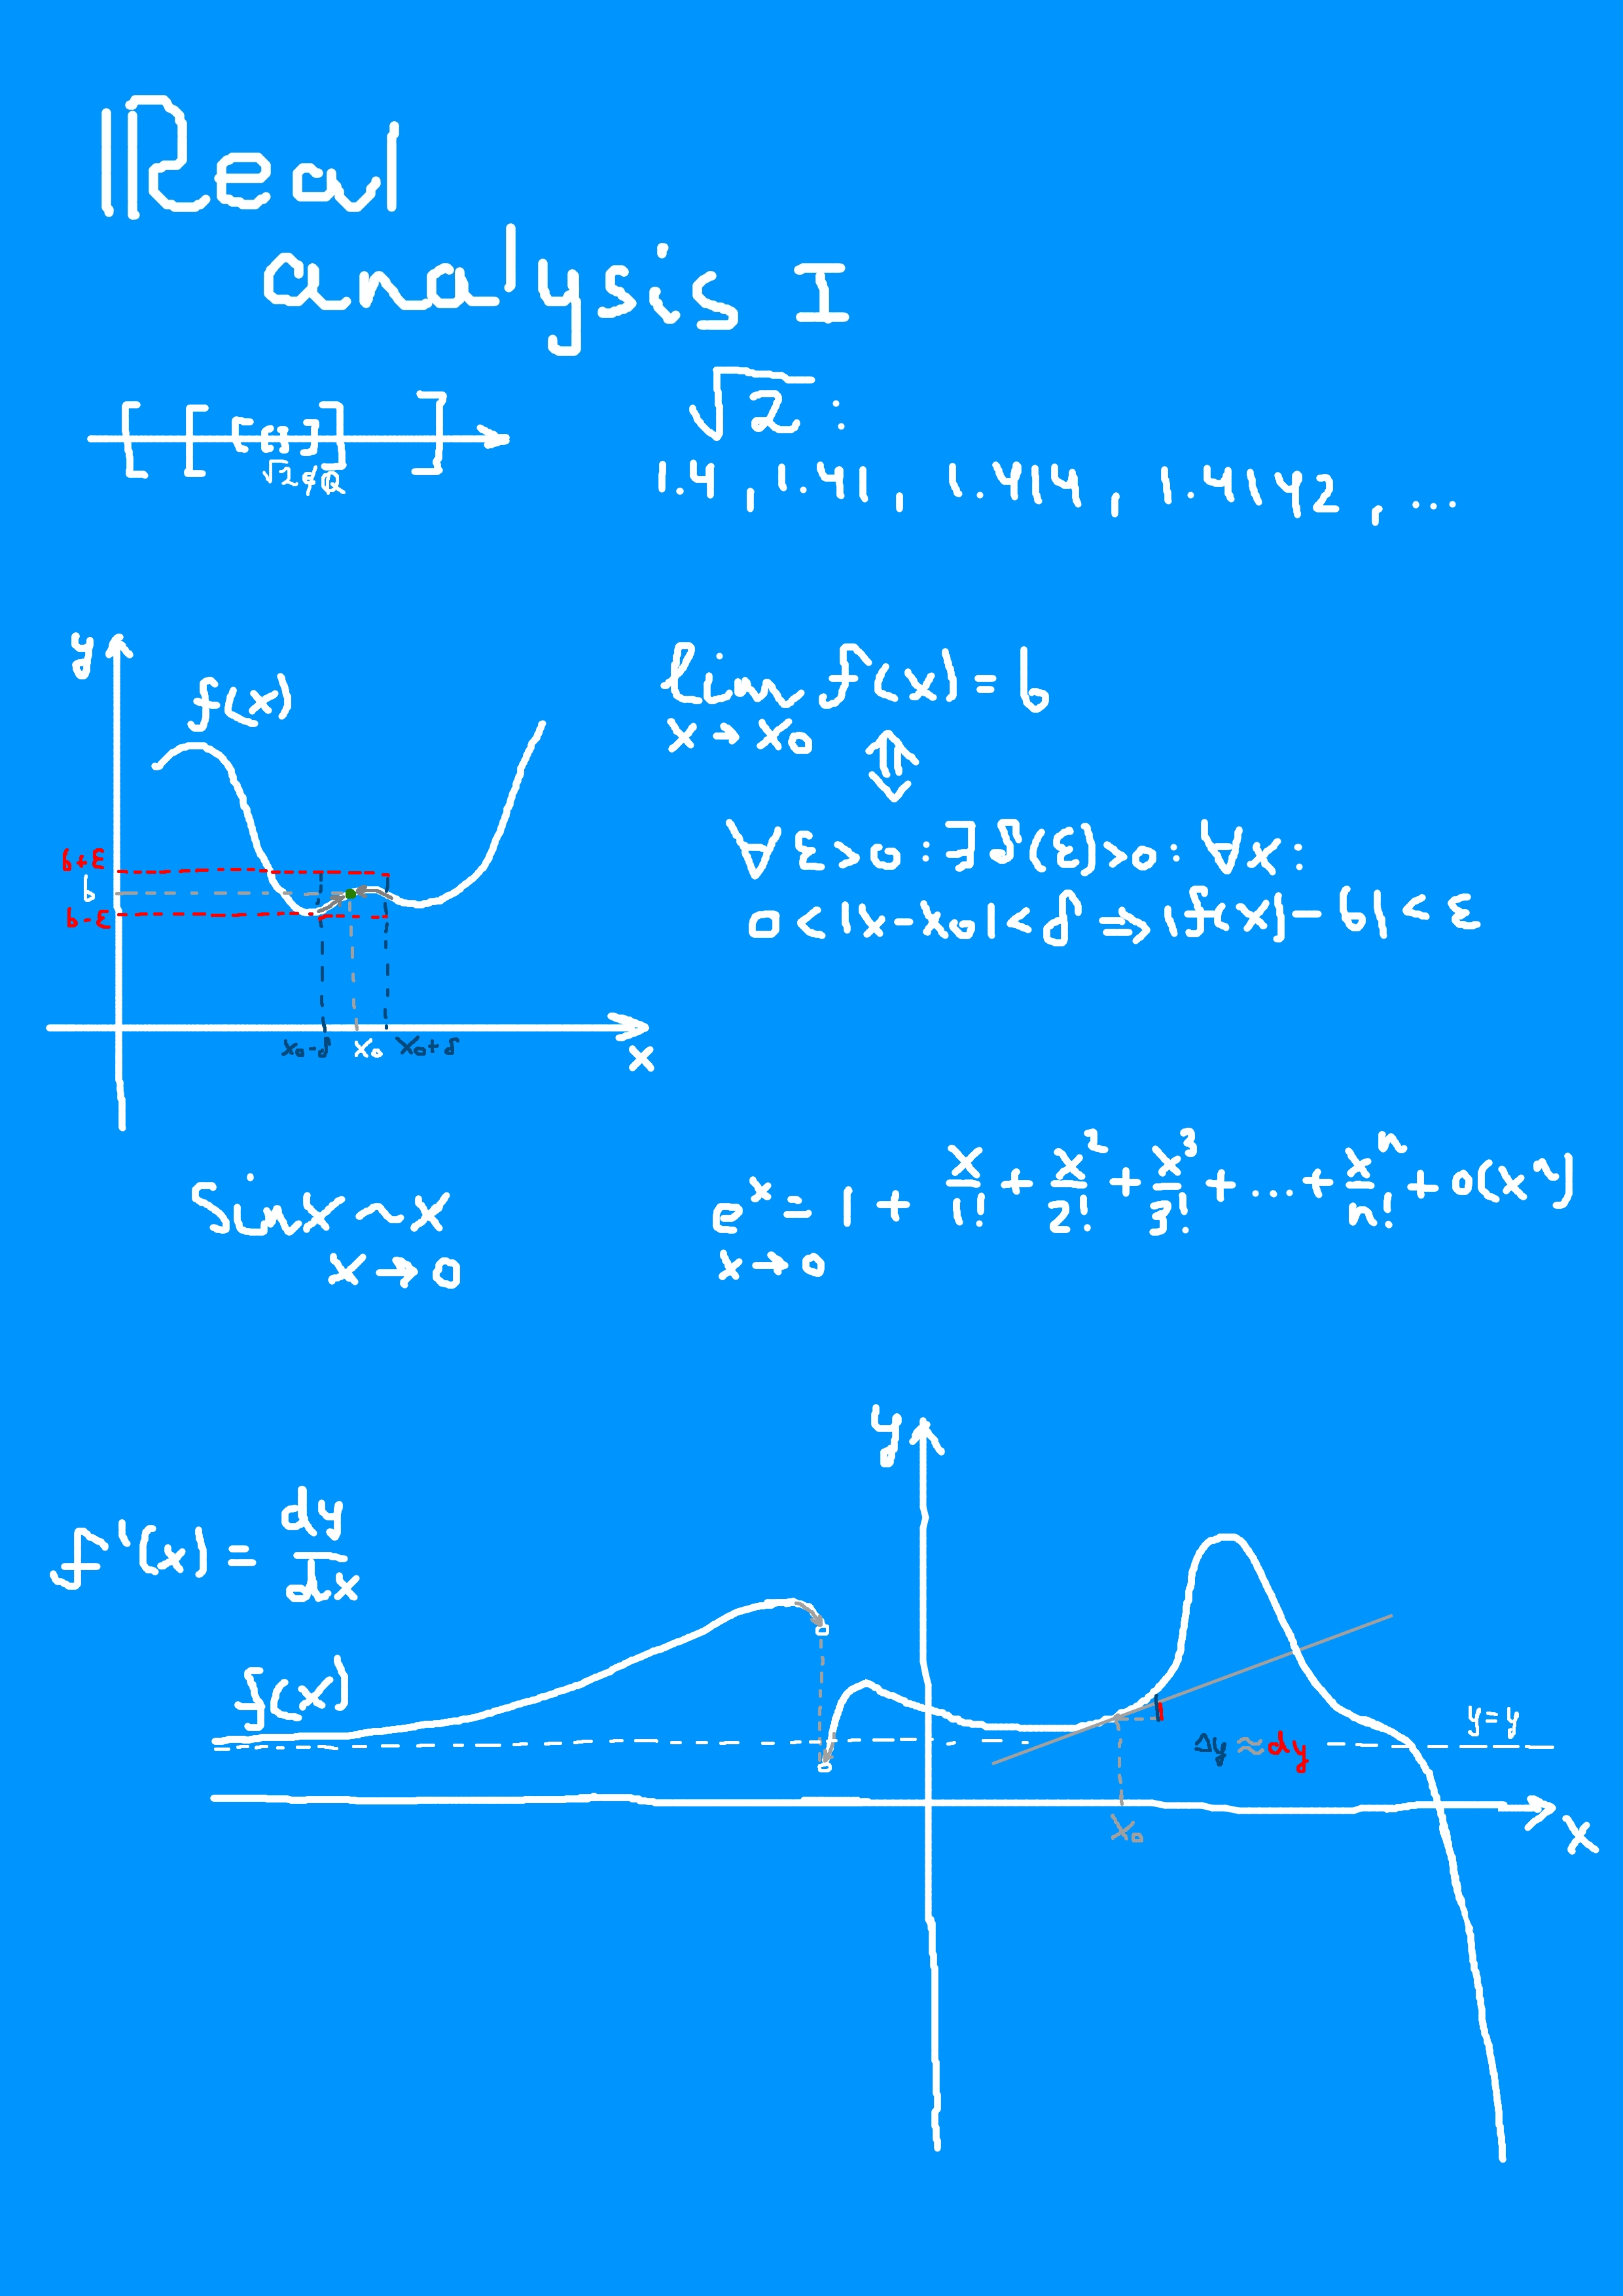
\includepdf{preview.jpg}
\tableofcontents
\newpage
\iffalse
\section{Невизначений інтеграл}
\subsection{Первісна, основні означення невизначеного інтегралу}

\begin{definition}
\textbf{Первісною} для функції $f: I \to \mathbb{R}$ називають функцію $F: I \to \mathbb{R}$, для якої
\begin{align*}
F'(x) = f(x)
\end{align*}
\end{definition}

\begin{example}
Зокрема $F(x) = x^2$ - первісна функції $f(x) = 2x$, тому що $F'(x) = (x^2)' = 2x = f(x)$. Проте це не єдина така первісна.
\end{example}

\begin{proposition}
Якщо $F(x), \Phi(x)$ - первісні для $f(x)$, то $\Phi(x) = F(x) + C$.\\
\textit{Випливає з наслідків теореми Лагранжа.}\\
\end{proposition}

\begin{definition}
Множину всіх первісних для функції $f(x)$ називають \textbf{невизначеним інтегралом} функції $f(x)$.\\
Позначення: $\huge \int f(x) \,dx = \{F(x): F'(x) = f(x)\}$.
\end{definition}

\begin{example}
$\huge\int 2x \,dx = \{x^2 + C | C \in \mathbb{R}\}$
\end{example}

\begin{remark}
Але надалі можна вважати, що $\huge \int f(x) \,dx = F(x) + C$, у разі якщо $F$ - первісна.\\
Тобто $\huge\int 2x\,dx = x^2 + C$.
\end{remark}

\begin{remark}
Взагалі-то кажучи, символ $\huge\int f(x)\,dx$ можна також використовувати, щоб позначити як первісну функції $f$, якщо не можна записати $F$ як функцію.\\
Зокрема $\huge\int e^{-x^2}\,dx$ - первісна функції $e^{-x^2}$, проте записати як функцію від змінної не можна.
\end{remark}

\begin{proposition}[Властивості]
1) $\huge \int f'(x)\,dx = f(x) + C$;\\
2) $\huge \left(\int f(x)\,dx \right)' = f(x)$; \\
Далі задамо функції $f,g$, які мають відповідно первісні $F,G$. Тоді:\\
3) $\alpha F$ - первісна для функції $\alpha f$ та $\huge \int \alpha f(x)\,dx = \alpha \int f(x)\,dx$;\\
4) $F+G$ - первісна для функції $f+g$ та $\huge \int f(x) + g(x) \,dx = \int f(x)\,dx + \int g(x)\,dx$.
\end{proposition}

\begin{proof}
1), 2) \textit{випливають з означення.} \bigskip \\
3) Якщо $F$ - первісна функції $f$, то тоді $\alpha F$ - первісна функції $\alpha f(x)$, тому що \\ $(\alpha F(x))' = \alpha F'(x) = \alpha f(x)$. \\ Отже, $\huge\int \alpha f(x) \,dx = \alpha F(x) + C = \alpha \left( F(x) + C^* \right) = \alpha \int f(x)\,dx$. \bigskip \\
4) Якщо $F,G$ - первісні відповідно функції $f,g$, то $F+G$ - первісна функції $f+g$, тому що \\ $(F(x)+G(x))' = F'(x)+G'(x) = f(x)+g(x)$. \\ Отже, $\huge\int f(x)+g(x) \,dx = F(x) + G(x) + C = F(x) + C^* + G(x) + C^{**} = \int f(x)\,dx + \int g(x)\,dx$.
\end{proof}

\begin{remark}
Підінтегральний вираз $f(x)\,dx$ варто розглядати як диференціал функції $F(x)$, тобто\\
$\huge\int f(x)\,dx = F(x) + C \iff d(F(x)+C) = f(x)\,dx$
\end{remark}

\subsubsection*{Таблиця первісних}
\begin{center}
\begin{tabular}{ c|c } 
 $f(x)$ & $F(x)$ \\
 \hline 
 $1$ & $x$ \\ [2ex]
 \hline 
 $x^\alpha$ & $\dfrac{x^{\alpha+1}}{\alpha+1}, \alpha \neq -1$ \\ [2ex]
 \hline
 $\dfrac{1}{x}$ & $\ln |x|$ \\ [2ex]
 \hline
 $\sin x$ & $-\cos x$\\ [2ex]
 \hline 
 $\cos x$ & $\sin x$\\ [2ex]
 \hline
 $\dfrac{1}{\cos^2 x}$ & $\tg x$\\ [2ex]
 \hline 
 $\dfrac{1}{\sin^2 x}$ & $-\ctg x$\\ [2ex]
 \hline
 $\dfrac{1}{\sqrt{1-x^2}}$ & $\arcsin x$\\ [2ex]
 \hline
 $\dfrac{1}{1+x^2}$ & $\arctg x$\\ [2ex]
 \hline
 $\dfrac{1}{\sqrt{1+x^2}}$ & $\ln(x+\sqrt{x^2+1})$\\ [2ex]
 \hline
 $e^x$ & $e^x$ \\ [2ex]
 \hline 
 $a^x$ & $\dfrac{a^x}{\ln a}$ \\ [2ex]
 \hline
 $\sh x$ & $\ch x$ \\ [2ex]
 \hline
 $\ch x$ & $\sh x$ \\ [2ex]
 \hline
 $\dfrac{1}{\ch^2 x}$ & $\th x$\\ [2ex]
 \hline
 $\dfrac{1}{\sh^2 x}$ & $-\cth x$\\
\end{tabular}
\end{center}

\begin{example}
Обчислимо $\huge\int (x+2)^2 + \tg^2 x\,dx$.\\
Робити будемо це, використовуючи таблицю первісних та властивості інтегралів.\\
$\huge\int (x+2)^2 + \tg^2 x\,dx = \int x^2 + 4x + 4 + \dfrac{1}{\cos^2 x} - 1\,dx = \int x^2\,dx + 4 \int x\,dx + 3 \int 1\,dx + \dfrac{1}{\cos^2 x}\,dx = \\ = \dfrac{x^3}{3} + 2x^2 + 3x + \tg x + C$.
\end{example}

\subsection{Заміна змінної}
\begin{theorem} Задано функцію $f: I \to \mathbb{R}$, має первісну $F$; функцію $g: J \to I$ - диференційована. Тоді $(f \circ g) g'$ має первісу $F \circ g$, причому \\
$\huge \int (f \circ g)(x) g'(x)\,dx = \int f(t)\,dt$.
\end{theorem}

\begin{proof}
Дійсно, $F \circ g$ - первісна для $(f \circ g) g'$, оскільки $(F \circ g)' (x) = F'(g(x)) g'(x) = f(g(x))g'(x)$. \\
Отже, $\huge \int f(g(x)) g'(x)\,dx = \int f(g(x)) \,dg(x) = \int f(t) \,dt = F(t) + C = F(g(x)) + C$.
\end{proof}

\begin{example} Обчислити $\huge \int \dfrac{1}{x \ln x} \,dx$\\
$\huge \int \dfrac{1}{x \ln x} \,dx \boxed{=} $ \hspace{2cm} Проведемо заміну: $\ln x = t$. Тоді $\dfrac{1}{x}\,dx = dt$\\
$\boxed{=} \huge \int \dfrac{1}{t}\,dt = \ln |t| + C = \ln |\ln x| + C$
\end{example}

\subsection{Інтегрування частинами}
\begin{theorem}
Задані функції $u,v: I \to \mathbb{R}$ - обида диференційовані. Відомо, що $u'v$ має первісну. Тоді $uv'$ також має первісну, причому\\
$\huge\int u(x)v'(x)\,dx = u(x)v(x) - \int v(x)u'(x)\,dx$.
\end{theorem}

\begin{proof}
Функція $u'(x)v(x)$ має первісну $H_1(x)$.\\
Тоді $u(x)v'(x)$ має первісну $H_2(x) = \huge u(x)v(x) - \int v(x)u'(x)\,dx$, тому що \\
$H_2'(x) = \huge \left( u(x)v(x) - \int v(x)u'(x)\,dx \right)' = (u(x)v(x))' - v(x)u'(x) = u'(x)v(x) + u(x)v'(x) - v(x)u'(x) = u(x)v'(x)$.\\
Отже, $\huge\int u(x)v'(x)\,dx = u(x)v(x) - \int v(x)u'(x)\,dx$.
\end{proof}

\begin{remark}
Більш зручно записати таку формулу: $\huge \int u\,dv = uv - \int v\,du$.
\end{remark}

\begin{example}
Обчислити $\huge \int x^2 e^x \,dx$.\\
$\huge \int x^2 e^x \,dx \boxed{=}$\\
$u = x^2 \Rightarrow du = 2x\,dx$\\
$e^x\,dx = dv \Rightarrow v = e^x$\\
$\boxed{=} x^2 e^x - \huge \int 2x e^x\,dx \boxed{\boxed{=}}$\\
$u = 2x \Rightarrow du = 2\,dx$\\
$e^x\,dx = dv \Rightarrow v = e^x$\\
$\boxed{\boxed{=}} x^2 e^x - (2xe^x - \huge \int 2e^x \,dx) = x^2 e^x - 2xe^x + 2e^x + C$
\end{example}

\subsection{Інтегрування дробово-раціональних функцій}
Розглянемо $\huge \int \dfrac{P(x)}{Q(x)}\,dx$, де $P(x), Q(x)$ - многочлени з дійсний коефіцієнтами. Є два випадки:\\
I. $\deg(P(x)) \geq \deg(Q(x))$\\
Тоді можемо поділити їх з остачею: $P(x) = S(x)Q(x) + R(x)$.\\
А тому $\huge \int \dfrac{P(x)}{Q(x)}\,dx = \int S(x) + \dfrac{R(x)}{Q(x)}\,dx$\\
,де $S(x)$ - деякий многочлен, який можна проінтегрувати таблицею, а також $\deg(R(x)) < \deg(Q(x))$. Зараз буде пункт, як такий випадок інтегрувати.
\bigskip \\
II. $\deg(R(x)) < \deg(Q(x))$\\
За наслідком основної теореми алгебри, розкладемо $Q(x)$ таким чином: \\
$Q(x) = (x-a_1)^{k_1} \dots (x-a_m)^{k_m} (x^2+p_1x+q_1)^{l_1} (x^2+p_sx+q_s)^{l_s}$. \\
Причому дискримінант квадратних трьохчленів - від'ємний. Тоді за теоремою десь із курсу ліналу, ми можемо $\dfrac{R(x)}{Q(x)}$ записати як суму простих дробів:\\
$\dfrac{R(x)}{Q(x)} = \dfrac{A_{11}}{x-a_1} + \dots + \dfrac{A_{1k_1}}{(x-a_1)^{k_1}}+ \dots + \dfrac{A_{m1}}{x-a_m} + \dots + \dfrac{A_{mk_m}}{(x-a_m)^{k_m}} + \\
+ \dfrac{B_{11}x + C_{11}}{x^2+p_1x+q_1} + \dots + \dfrac{B_{1l_1}x + C_{1l_1}}{(x^2+p_1x+q_1)^{l_1}} + \dots + \dfrac{B_{s1}x + C_{s1}}{x^2+p_sx+q_s} + \dots + \dfrac{B_{sl_s}x + C_{sl_s}}{(x^2+p_sx+q_s)^{l_s}}$.\\
Коротше, залишається розглянути 4 вигляди інтегралу:
\bigskip \\
1) $\huge \int \dfrac{1}{x-a}\,dx = \ln|x-a| + C$
\bigskip \\
2) $\huge \int \dfrac{1}{(x-a)^k}\,dx = \int (x-a)^{-k}\,dx = \dfrac{(x-a)^{-k+1}}{-k+1} + C = \dfrac{1}{(1-k)(x-a)^{k-1}} + C$
\bigskip \\
3) $\huge \int \dfrac{Bx+C}{x^2+px+q}\,dx \boxed{=}$\\
Знаменник розпишу як $x^2 + px + q = \left(x + \dfrac{p}{2} \right)^2 + \dfrac{4q-p^2}{4}$.\\
Зробимо заміну: $x + \dfrac{p}{2} = t \Rightarrow dx = dt$\\
Також $Bx+C = Bt - B\dfrac{p}{2} + C$.\\
Перепозначення: $\dfrac{4q-p^2}{4} = a^2 > 0 \hspace{0.5cm} C - B \dfrac{p}{2} = M$.\\
$\boxed{=} \huge \int \dfrac{Bt + M}{t^2 + a^2}\,dt = B \int \dfrac{t}{t^2+a^2}\,dt + M \int \dfrac{1}{t^2+a^2}\,dt \boxed{\boxed{=}}$\\
$\huge \int \dfrac{t}{t^2+a^2}\,dt = \dfrac{dt^2}{2(t^2+a^2)} = \dfrac{1}{2} \ln|t^2+a^2|$\\
$\huge \int \dfrac{1}{t^2+a^2}\,dt = \dfrac{1}{a^2} \int \dfrac{1}{1 + \left(\frac{t}{a}\right)^2}\,dt = \dfrac{1}{a} \int \dfrac{d \frac{t}{a}}{1 + \left(\frac{t}{a}\right)^2} = \dfrac{1}{a} \arctg \dfrac{t}{a}$\\
$\boxed{\boxed{=}} \huge \frac{B}{2} \ln|t^2+a^2| + \frac{M}{a} \arctg \frac{t}{a} + C$\\
Ну а далі робимо зворотню заміну - інтеграл розв'язаний.
\bigskip \\
4) $\huge \int \dfrac{Bx+C}{(x^2+px+q)^l}\,dx \boxed{=}$\\
Тут робимо ті самі заміни, що в 3)\\
$\boxed{=} \huge \int \dfrac{Bt+M}{(t^2+a^2)^l}\,dt = B \int \dfrac{t}{(t^2+a^2)^l} \,dt + M \int \dfrac{1}{(t^2+a^2)^l}\,dt$\\
Ну і тут я ланцюг рівностей зупиню, якщо перший інтеграл - ще ок, то другий - це дупа\\
$\huge \int \dfrac{t}{(t^2+a^2)^l}\,dt = \int \dfrac{dt^2}{2(t^2+a^2)^l}\,dt = \dfrac{1}{2} \dfrac{1}{(1-l)s^{l-1}}$ \bigskip \\
$\huge \int \dfrac{1}{(t^2+a^2)^l}\,dt \boxed{=} \hspace{2cm} u = \dfrac{1}{(t^2+a^2)^l} \hspace{1cm} dv = dt$\\
$\boxed{=} \huge \dfrac{t}{(t^2+a^2)^l} + 2l \int \dfrac{t^2}{(t^2+a^2)^{l+1}}\,dt + \dfrac{t}{(t^2+a^2)^l} + 2l \left(\int \dfrac{dt}{(t^2+a^2)^l} - a^2 \dfrac{dt}{(t^2+a^2)^{l+1}} \right)$\\
Позначимо за $I_l = \huge \int \dfrac{t}{(t^2+a^2)^l}\,dt$\\
Тоді маємо таке рівняння:\\
$I_l = \dfrac{t}{(t^2+a^2)^l} + 2l \cdot I_l - 2la^2 \cdot I_{l+1}$\\
Залишилось виразити $I_{l+1}$ та розв'язати рівняння рекурсивно, причому $I_1$ ми вже рахували.
\bigskip \\
Все! Інтеграл $\huge\int \dfrac{P(x)}{Q(x)}\,dx$ - розв'язаний.
\bigskip \\

\begin{example}
Обчислити $\huge \int \dfrac{x^4}{1+x^3}\,dx$\\
Оскільки $\deg(x^4) > \deg(1+x^3)$, то ми поділимо многочлени. Отримаємо:\\
$\huge \int \dfrac{x^4}{1+x^3}\,dx = \int x - \dfrac{x}{x^3+1}\,dx = x^2 - \int \dfrac{x}{x^3+1}\,dx$.\\
Обчислимо другий інтеграл. Перед цим розкладемо дріб на суму простих дробів методом невизначених коефіцієнтів:\\
$\dfrac{x}{x^3+1} = \dfrac{x}{(x+1)(x^2-x+1)} = \dfrac{A}{x+1} + \dfrac{Bx+C}{x^2-x+1} \boxed{=}$\\
$A(x^2-x+1) + (Bx+C)(x+1) = x$\\
$\Rightarrow \begin{cases}
A + B = 0 \\
-A + B + C = 1\\
A + C = 0
\end{cases} \Rightarrow A = -\dfrac{1}{3}, B = \dfrac{1}{3}, C = \dfrac{1}{3}$\\
$\boxed{=} -\dfrac{1}{3(x+1)} + \dfrac{1}{3} \dfrac{x+1}{x^2-x+1}$\\
Таким чином, треба порахувати такий інтеграл:\\
$\huge \int \dfrac{x}{x^3+1}\,dx = -\frac{1}{3} \int \frac{1}{x+1}\,dx + \frac{1}{3} \int \frac{x+1}{x^2-x+1}\,dx \boxed{=}$\\
І розглянемо другий інтеграл:\\
$\huge \int \frac{x+1}{x^2-x+1}\,dx = \int \frac{4x+4}{(2x-1)^2 + 3}\,dx = \int \frac{4x-2}{(2x-1)^2 +3}\,dx + \int \frac{6}{(2x-1)^2 +3}\,dx = \\ = \ln((2x-1)^2+3) + 6 \dfrac{1}{2\sqrt{3}} \arctg \dfrac{2x-1}{\sqrt{3}} = \ln(4x^2-4x+4) + \sqrt{3} \arctg \dfrac{2x-1}{\sqrt{3}}$\\
$\boxed{=} \huge -\dfrac{1}{3} \ln|x+1| + \dfrac{1}{3} \ln(4x^2-4x+4) + \dfrac{1}{\sqrt{3}} \arctg \dfrac{2x-1}{\sqrt{3}}$\\
Разом отримаємо:\\
$\huge \int \dfrac{x^4}{1+x^3}\,dx = x^2 + \dfrac{1}{3} \ln|x+1| - \dfrac{1}{3} \ln(4x^2-4x+4) - \dfrac{1}{\sqrt{3}} \arctg \dfrac{2x-1}{\sqrt{3}} + C$
\end{example}

\begin{example}
Обчислити $\huge\int \dfrac{1}{(x^2+1)^2}\,dx$\\
Можна скористатися отриманою рекурентною формулою, а можна зробити ті самі кроки.\\
$\huge \int \dfrac{1}{(x^2+1)^1}\,dx = \arctg x$\\
$\huge \int \dfrac{1}{(x^2+1)^1}\,dx \overset{u=\text{дріб}, dv = dx}{=} \dfrac{x}{x^2+1} + \int \dfrac{2x^2}{(x^2+1)^2}\,dx = \dfrac{x}{x^2+1} + 2\int \dfrac{1}{x^2+1} - \dfrac{1}{(x^2+1)^2}\,dx$\\
$\implies \huge \arctg x = \dfrac{x}{x^2+1} + 2\arctg x - 2 \int \dfrac{1}{(x^2+1)^2}\,dx$\\
$\huge\int \dfrac{1}{(x^2+1)^2}\,dx = \dfrac{1}{2} \arctg x + \dfrac{x}{2(x^2+1)} + C$
\end{example}

\subsection{Інтегрування тригонометричних функцій}
I. Розглянемо $\huge \int \sin^k x \cos^m x \,dx \hspace{0.5cm}$, де $k,m \in \mathbb{Z}$. Маємо такі заміни:\\
1) $k$ - непарне, тобто $k = 2l+1$, тоді заміна: $\cos x = t$. Тому\\
$(-\sin x) \,dx = dt$ і $\sin^2 x = 1 - \cos ^2x = 1 - t^2$\\
$\huge \int \sin^k x \cos^m x \,dx = \int \sin^{2l+1} x t^m \dfrac{dt}{-\sin x} = -\int t^m (1-t^2)^l\,dt$
\bigskip \\
2) $m$ - непарне, тобто $m = 2l+1$, тоді заміна: $\sin x = t$. Тому\\
$\cos x \,dx = dt$ і $\cos^2 x = 1 - \sin^2 x = 1 - t^2$\\
$\huge \int \sin^k x \cos^m x \,dx = \int t^k \cos^{2l+1}x \dfrac{dt}{\cos x} = \int t^k(1-t^2)^l \,dt$
\bigskip \\
3) $k,m$ - парні, тобто $k=2l, m =2n$, тоді знижуємо степені: \\ $\sin^2 x = \dfrac{1-\cos 2x}{2} \hspace{0.5cm} \cos^2 x = \dfrac{1+\cos 2x}{2}$\\
$\huge \int \sin^k x \cos^m x \,dx = \int \left( \dfrac{1-\cos 2x}{2} \right)^l \left( \dfrac{1+\cos 2x}{2} \right)^n \,dx$
\bigskip \\
Всі отримані інтеграли є випадком інтегрування дробово-раціональних виразів.

\begin{example}
Обчислити $\huge\int \cos^3 x \,dx$\\
Заміна: $t = \sin x$, випадок 2), тоді $dt = \cos x \,dx$\\
$\huge\int \cos^3 x \,dx = \int (1-t^2)\,dx = t - \dfrac{t^3}{3} + C = \sin x - \dfrac{\sin^3 x}{3} + C$
\end{example}

II. Розглянемо $\huge \int R(\sin x, \cos x)\,dx \hspace{0.5cm}$, де $R$ - дробово-раціональний вираз від $\sin x, \cos x$. Маємо таку заміну:\\
$t = \tg \dfrac{x}{2} \implies x = 2 \arctg t \implies dx = \dfrac{2}{1+t^2}\,dt$\\
$\sin x = \dfrac{2 \tg \frac{x}{2}}{1 + \tg^2 \frac{x}{2}} = \dfrac{2t}{1+t^2}$\\
$\cos x = \dfrac{1 - \tg^2 \frac{x}{2}}{1 + \tg^2 \frac{x}{2}} = \dfrac{1-t^2}{1+t^2}$\\
$\huge \int R(\sin x, \cos x)\,dx = \int R\left(\dfrac{2t}{1+t^2}, \dfrac{1-t^2}{1+t^2} \right) \cdot \dfrac{2}{1+t^2}\,dt$\\
Отримуємо випадок інтегрування дробово-раціональних виразів.

\begin{example}
Обчислити $\huge \int \dfrac{dx}{5-3\cos x}$\\
Заміна: $t = \tg \dfrac{x}{2}$, випадок II. Тоді беремо решта замін звідси, з нашого пункту.\\
$\huge \int \dfrac{dx}{5-3\cos x} = \int \dfrac{1}{5-3 \frac{1-t^2}{1+t^2}} \dfrac{2}{1+t^2}\,dt = \int \dfrac{2\,dt}{5+5t^2-3+3t^2} = \int \dfrac{dt}{4t^2+1} = \dfrac{1}{2} \arctg 2t + C = \\ = \dfrac{1}{2} \arctg \left(2 \tg \dfrac{x}{2} \right) + C$
\end{example}

\subsection{Інтегрування ірраціональних виразів}

I. Розглянемо $\huge \int R\left( \sqrt[k_1]{\dfrac{ax+b}{cx+d}}, \dots, \sqrt[k_n]{\dfrac{ax+b}{cx+d}} \right)\,dx$, де $R$ - дробово-раціональний вираз, причому $ad-cb \neq 0$.\\
Нехай $m = \textrm{LCM} (k_1,\dots,k_n)$. Спрацює заміна: $\dfrac{ax+b}{cx+d} = t^m$\\
Виразимо $x$ з цього рівняння:\\
$ax+b =t^m cx + t^m d \Rightarrow x = \dfrac{t^md-b}{a-ct^m}$\\
Тоді $dx = \dfrac{dmt^{m-1}(a-ct^m) + (t^md-b)cmt^{m-1}}{(a-ct^m)^2}\,dt = \dfrac{mt^{m-1}(ad-bc)}{(a-ct^m)^2}\,dt$\\
$\huge \int R\left( \sqrt[k_1]{\dfrac{ax+b}{cx+d}}, \dots, \sqrt[k_n]{\dfrac{ax+b}{cx+d}} \right)\,dx = \int R(t^{m_1},\dots,t^{m_n}) \dfrac{mt^{m-1}(ad-bc)}{(a-ct^m)^2}\,dt$,\\
де $m_1 = \dfrac{m}{k_1},\dots,m_n = \dfrac{m}{k_n} \in \mathbb{Z}$\\
Отримаємо інтеграл дробово-раціонального виразу.

\begin{example}
Обчислити $\huge \int \dfrac{\sqrt{x+1}+2}{(x+1)^2 - \sqrt{x+1}}\,dx$\\
Заміна: $t^2 = x+1$. Тоді $x = t^2 -1 \Rightarrow dx = 2t \,dt$\\
$\huge \int \dfrac{\sqrt{x+1}+2}{(x+1)^2 - \sqrt{x+1}}\,dx = \int \dfrac{t+2}{t^4-t} \cdot 2t\,dt = 2 \int \dfrac{t+2}{t^3-1}\,dt \boxed{=}$\\
обчислення цього інтегралу проводиться як в п. 4, тому я пропускаю цей момент\\
$\boxed{=} -\ln(t^2+t+1) - \dfrac{2}{\sqrt{3}} \arctg \dfrac{2t+1}{\sqrt{3}} + 2 \ln|t-1|+ C = \\
= -\ln(x+2+\sqrt{x+1}) - \dfrac{2}{\sqrt{3}} \arctg \dfrac{2\sqrt{x+1}+1}{\sqrt{3}} + 2 \ln|\sqrt{x+1}-1| + C$
\end{example}

II. Розглянемо такі інтеграли:\\
1) $\huge \int R(x,\sqrt{a^2-x^2})\,dx \boxed{=}$\\
Заміна: $x = a\sin t \Rightarrow dx = a\cos t \,dt$\\
$\boxed{=} \huge \int R(a\sin t, a\cos t) \cdot a\cos t \,dt$
\bigskip \\
2) $\huge \int R(x,\sqrt{a^2+x^2})\,dx \boxed{=}$\\
Заміна: $x = a\tg t \Rightarrow dx = \dfrac{a}{\cos^2 t} dt$\\
$\boxed{=} \huge \int R\left(a\tg t, \dfrac{a}{\cos t}\right) \cdot \dfrac{a}{cos^2 t} \,dt$
\bigskip \\

\iffalse
Або інша заміна: $x = a \sh t \Rightarrow dx = a \ch t \,dt$\\
$\boxed{=} \huge \int R(a\sh t, a \ch t) \cdot a \ch t\,dt$
\bigskip \\
\fi

3) $\huge \int R(x, \sqrt{x^2-a^2})\,dx \boxed{=}$\\
Заміна: $x = \dfrac{a}{\cos t} \Rightarrow dx = \dfrac{a}{\cos^2 t} \sin t\,dt$\\
$\boxed{=} \huge \int R \left(\dfrac{a}{\cos t}, a \tg t \right) \cdot \dfrac{a \sin t}{\cos ^2 t}\,dt$
\bigskip \\

\iffalse
Або інша заміна: $x = a \ch t \Rightarrow dx = a \sh t \,dt$\\
$\boxed{=} \huge \int R(a \ch t, a \sh t) \cdot a \sh t \,dt$
\bigskip \\
\fi
Усі отримані інтеграли II є інтегралами тригонометричних функцій.

\begin{example}
Обчислити $\huge \int \sqrt{4-x^2}\,dx$\\
Заміна: $x = 2\sin t$, випадок 1). Тоді $dx = 2 \cos t \,dt$\\
$\huge \int \sqrt{4-x^2}\,dx = \int 2 \cos t \cdot 2 \cos t \,dt = \int 2(1+\cos 2t)\,dt = 2t + \sin 2t + C = 2t + 2 \sin t \cos t + C = \\ = 2 \arcsin \frac{x}{2} + 2 \frac{x}{2} \sqrt{1-\frac{x^2}{4}}+C = 2 \arcsin \frac{x}{2} + \dfrac{x \sqrt{4-x^2}}{2} + C$
\end{example}

\subsection{Диференціальний біном}
Розглянемо $\huge \int x^m (ax^n + b)^p\,dx \hspace{1cm}$, де $m,n,p \in \mathbb{Q}$. Маємо три випадки:\\
1) $p \in \mathbb{Z}$, тоді маємо: \\
$m = \dfrac{p_1}{q_1}; n = \dfrac{p_2}{q_2}$.\\
Нехай $q = \textrm{LCM}(q_1,q_2)$. Тоді заміна: $x = t^q$.
\bigskip \\
2) $p \not \in \mathbb{Z}$, але $\dfrac{m+1}{n} \in \mathbb{Z}$, тоді маємо:\\
$p = \dfrac{j}{l}$.\\
Тоді заміна: $ax^n+b = t^l$.
\bigskip \\
3) $p \not \in \mathbb{Z}$, $\dfrac{m+1}{n} \not \in \mathbb{Z}$, але $p+ \dfrac{m+1}{n} \in \mathbb{Z}$, тоді маємо: \\ 
$p = \dfrac{j}{l}$.\\
Тоді заміна: $a+bx^{-n} = t^l$.
\bigskip \\
Заміни в 1), 2), 3) називають \textbf{підстановками Чебишова}, що призводять до інтегралу дробово-раціональних виразів.\\
Якщо жодна з пунктів не спрацьовує, то інтеграл не може бути обчисленим через елементарні функції (залишаю поки це як факт).
\begin{example}
Обчислити $\huge \int \sqrt[3]{x-x^3}\,dx = \int x^{\frac{1}{3}} (1-x^2)^\frac{1}{3}\,dx$\\
Тут у нас $m = \dfrac{1}{3}$, $n = 2$, $p = \dfrac{1}{3}$\\
Спрацьовує 3), тому що $p + \dfrac{m+1}{n} = \dfrac{1}{3} + \dfrac{1+\frac{1}{3}}{2} = 1 \in \mathbb{Z}$\\
Заміна: $-1+x^{-2}=t^3$\\
$-2x^{-3}\,dx = 3t^2\,dt$\\
$\huge \int \sqrt[3]{x-x^3}\,dx = \int x^{\frac{1}{3}} (1-x^2)^\frac{1}{3}\,dx = \int (x^{-2}-1)^{\frac{1}{3}} x^{\frac{2}{3}} x^{\frac{1}{3}}\,dx = \int t \cdot x \cdot \frac{3t^2 x^3 \,dt}{-2} = \int \frac{3t^3\,dt}{-2(t^3+1)^2} = \\ = \frac{3}{-2} \left(\int \frac{dt}{t^3+1} - \int \frac{dt}{(t^3+1)^2} \right) \boxed{=}
$\\
обчислення цього інтегралу проводиться як в п. 4, тому я пропускаю цей момент\\
$\boxed{=} \huge -\frac{\ln|t+1|}{2} + \frac{\ln(t^2-t+1)}{4} - \frac{\sqrt{3}}{2} \arctg \frac{2x-1}{\sqrt{3}} + \frac{\ln |t+1|}{3} - \frac{\ln(t^2-t+1)}{6} + \frac{\sqrt{3}}{3} \arctg \frac{2x-1}{\sqrt{3}} + \frac{t}{2t^3+2} + C =\\
= - \frac{1}{6} \ln|t+1| + \frac{1}{12} \ln(t^2-t+1) - \frac{\sqrt{3}}{6} \arctg \frac{2x-1}{\sqrt{3}} + \frac{t}{2t^3+2} + C$\\
І підставляємо $t = \sqrt[3]{x^{-2}+1}$.
\end{example}
\newpage
\fi

\iffalse
\section{Визначений інтеграл}
\subsection{Підхід Рімана}
\begin{definition}
\textbf{Розбиттям} множини $[a,b]$ називають множину точок $\tau = \{x_0,x_1,\dots,x_{n-1},x_n\}$, для яких
\begin{align*}
a = x_0 < x_1 < \dots < x_{n-1} < x_{n} = b
\end{align*}
\end{definition}

\begin{definition}
Позначимо за $\Delta x_1 = x_1 - x_0, \dots, \Delta x_n = x_{n} - x_{n-1}$. Тоді числом
\begin{align*}
|\tau| = \max\{\Delta x_1,\dots, \Delta x_n\}
\end{align*}
називають \textbf{діаметром} (або \textbf{дрібністю}) розбиття $\tau$.
\end{definition}

\begin{definition}
Задані розбиття $\tau, \tau'$ відрізка $[a,b]$. Якщо $\tau \subset \tau'$, то $\tau'$ називають \textbf{підрозбиттям} розбиття $\tau$.
\end{definition}

\begin{proposition}
Задано $\tau'$ - підрозбиття для $\tau$. Тоді $|\tau'| \leq |\tau|$.
\end{proposition}

\begin{proof}
Дійсно, із розбиття ми можемо отримати підрозбиття шляхом додавання точок. Тоді деякі інтервали будуть ділитись на підінтервали через додавання точки. Відповідно діаметр зменшується.
\end{proof}

\begin{definition}
Задано $\tau = \{x_0,x_1,\dots,x_n\}$ - розбиття відрізка $[a,b]$\\
Елементи множини $\xi = \{\xi_1, \dots, \xi_n \}$ називають \textbf{відміченими точками}.\\
Тут $\xi_1 \in [x_0,x_1), \xi_2 \in [x_1,x_2), \dots, \xi_n \in [x_{n-1}, x_n]$
\end{definition}

\begin{definition}
Задано функцію $f: [a,b] \to \mathbb{R}$, розбиття $\tau = \{x_0,x_1,\dots,x_n\}$ та відмічені точки $\xi = \{\xi_1, \dots, \xi_n \}$.\\
\textbf{Інтегральною сумою Рімана} функції $f$ для нашого розбиття $\tau$ та відмічених точок називають число:
\begin{align*}
\sigma (f, \tau, \xi) = \sum_{k=1}^n f(\xi_k) \Delta x_k
\end{align*}
\end{definition}

\begin{figure}[H]
\centering
\begin{tikzpicture}
\draw[thick] (1,-1pt)--(1,1pt) node[anchor = north] {$x_0$};
\draw[thick] (2,-1pt)--(2,1pt) node[anchor = north] {$x_1$};
\draw[thick] (4,-1pt)--(4,1pt) node[anchor = north east] {$x_{n-1}$};
\draw[thick] (5,-1pt)--(5,1pt) node[anchor = north] {$x_n$};


\draw[fill = black!30] (1,0) rectangle (2, {exp((1.5-2)/3)});
\draw[fill = black!30] (4,0) rectangle (5, {exp((4.5-2)/3)});

\draw[thick, dashed] (1.5,{exp((1.5-2)/3)})--(1.5,0) node[anchor = north, scale = 0.8] {$\xi_1$};
\draw[thick, dashed] (4.5,{exp((4.5-2)/3)})--(4.5,0) node[anchor = north, scale = 0.8] {$\xi_n$};

\draw[thick, ->] (-0.5,0)--(5.5,0) node[anchor = north] {$x$};
\draw[thick, ->] (0,-0.5)--(0,3) node[anchor = east] {$y$};

\draw[thick, domain=1:5, variable=\x, samples = 1000] plot({\x}, {exp((\x-2)/3)});
%node[anchor = south east, scale = 0.8] {$f(x) = \dfrac{\sin x}{x}$};
%\node[white] at (0,1) [circle,fill,inner sep=1.5pt, draw = black]{};
%\node[black] at (0,0) [circle,fill,inner sep=1.5pt, draw = black]{};
\end{tikzpicture}
\end{figure}

\begin{definition}
Задано функцію $f: [a,b] \to \mathbb{R}$.\\
Функція $f$ називається \textbf{інтегрованою за Ріманом} на $[a,b]$, якщо існує таке число $I \in \mathbb{R}$, для якого виконана умова:
\iffalse
\begin{align*}
\forall \varepsilon > 0: \exists \tau_{\varepsilon}: \forall \tau \supset \tau_{\varepsilon}: \forall \xi^{\tau}: \abs{S_{\tau,\xi^{\tau}}(f) -I}<\varepsilon
\end{align*}
\fi

\begin{align*}
\forall \varepsilon > 0: \exists \delta(\varepsilon) > 0: \forall (\tau, \xi): |\tau| < \delta \implies \abs{\sigma(\tau, \xi, f) - I} < \varepsilon
\end{align*}
Число $I$ називають \textbf{інтегралом Рімана}.
\begin{align*}
I = \int_a^b f(x)\,dx
\end{align*}
Позначення: $I = \huge\lim_{|\tau| \to 0} \sigma(f, \tau, \xi)$ (нелегально, тому що не знаю, що таке границя за базою).\\
Множина інтегрованих функцій за Ріманом: $\mathcal{R}([a,b])$.
\end{definition}

\begin{remark}
Для кожного розбиття $\tau$, ми можемо самі обирати точки $\xi$, просто головне, щоб $|\tau| < \delta$.
\end{remark}

\begin{example}
Доведемо, що функція $f(x) = 1 \in \mathcal{R}([a,b])$, а також $\huge \int_a^b 1\,dx = b-a$.\\
Для початку зафіксуємо розбиття $\tau = \{x_0,x_1,\dots,x_n\}$ та відмітимо точки $\xi = \{\xi_1,\dots,\xi_n\}$. Це аби знайти інтегральну суму:\\
$\sigma (f, \tau, \xi) = \huge \sum_{k=1}^n f(\xi_k) \Delta x_k$\\
$\sigma (1, \tau, \xi) = \huge \sum_{k=1}^n \Delta x_k = x_1 - x_0 + x_2 - x_1 + \dots + x_n - x_{n-1} = x_n - x_0 = b - a$.\\
І ця інтегральна сума має це значенням при довільному розбитті. Якщо встановити $I = b -a$, то тоді:\\
$\forall \varepsilon > 0: \exists \delta(\varepsilon) > 0: \forall (\tau, \xi): |\tau| < \delta \implies |\sigma (\tau, \xi, f) - I| = |b-a - (b-a)| = 0 < \varepsilon$.\\
Отже, $f(x) = 1 \in \mathcal{R}([a,b])$, а інтеграл $\huge \int_a^b 1\,dx = b-a$.
\end{example}

\iffalse
\begin{example}
Доведемо, що функція $f(x) = \mathbbm{1}_{x^*}(x) \in \mathcal{R}([a,b])$, причому $x^* \in [a,b]$. Також покажемо, що $\huge \int_a^b 1_{x^*} (x)\,dx = 0$.\\
Для початку зафіксуємо розбиття $\tau = \{x_0,x_1,\dots,x_n\}$ та відмітимо точки $\xi^\tau = \{\xi_1,\dots,\xi_n\}$. Знаходимо інтегральну суму:\\
Якщо виявиться, що $x^* \not \in \xi^\tau$, то $\forall k = 1,\dots, n: 1_{x^*}(\xi_k) = 0$. Отже, $S = 0$.\\
А якщо $x^* \in \xi^\tau$, то існує єдина точка $\xi_m \in \tau$, що $x^* = \xi_m$. Тоді $\forall k \neq m: 1_{x^*}(\xi_k) = 0$, а тоді $S = \Delta x_m = x_m - x_{m-1}$\\
Для другого випадку якщо покласти $I = 0$, то:\\
$\forall \varepsilon > 0: \exists \delta < \varepsilon: \forall (\tau, \xi^{\tau}): |\tau| < \delta \implies |S_{\tau,\xi^\tau}(f)-I| = |x_m-x_{m-1}|<\varepsilon$
\end{example}
\fi

\iffalse
\ex{7.1.10.} Доведемо, що функція $1_{\mathbb{Q}} \not \in R([a,b])$\\
Знайдемо інтегральні суми:\\
Якщо взяти всі точки $\xi_k \in \Delta_k \cap \mathbb{Q}$, то $\forall k = 1,\dots,n: 1_{\mathbb{Q}}(\xi_k) = 1$\\
$\Rightarrow S_{\tau, \xi^\tau}(1_{\mathbb{Q}}) = (x_1-x_0)+\dots+(x_n-x_{n-1}) = b-a$\\
Проте коли всі точки $\xi_k \in \Delta_k \setminus \mathbb{Q}$, то $\forall k = 1,\dots,n: 1_{\mathbb{Q}}(\xi_k) = 0$\\
$\Rightarrow S_{\tau, \xi^\tau}(1_{\mathbb{Q}}) = 0$\\
Отримані значення не залежать від розбиття, але залежить від відмічених точок. Тобто однозначно задати $I$ ми не можемо. Отже, $1_{\mathbb{Q}} \not \in R([a,b])$
\fi

\begin{theorem}
Задано функцію $f: [a,b] \to \mathbb{R}$.\\
Число $I$ - інтеграл Рімана $\iff \forall (\tau_n, \xi_n): |\tau_n| \overset{n \to \infty}{\longrightarrow} 0 \implies \sigma(f, \tau_n, \xi_n) \overset{n \to \infty}{\longrightarrow} I$.\\
\textit{Зрозуміло. Фактично, це можна вважати як означення 'за Гейне', але не зовсім. Проте схожі.}
\end{theorem}

\subsection{Суми Дарбу}
\begin{definition}
Задано функцію $f: [a,b] \to \mathbb{R}$ - обмежена. Визначмо такі значення для розбиття $\tau = \{x_0,x_1,\dots,x_n\}$:
\begin{align*}
m_k = \inf_{x \in [x_{k-1},x_k]} f(x) \hspace{2cm} M_k = \sup_{x \in [x_{k-1},x_k]} f(x) \hspace{0.5cm} k=1,\dots,n
\end{align*}
\textbf{Верхньою та нижньою сумою Дарбу} називають такі суми:
\begin{align*}
U(f, \tau) = \sum_{k=1}^n M_k \Delta x_k \hspace{2cm} L(f,\tau) = \sum_{k=1}^n m_k \Delta x_k \hspace{2cm}
\end{align*}
\end{definition}
\begin{figure}[H]
\centering
\begin{tikzpicture}
\draw[thick] (1,-1pt)--(1,1pt) node[anchor = north] {$x_0$};
\draw[thick] (2,-1pt)--(2,1pt) node[anchor = north] {$x_1$};
\draw[thick] (5,-1pt)--(5,1pt) node[anchor = north] {$x_n$};
\foreach \i in {1,2,3,4}
	\draw[fill = black!30] (\i,0) rectangle (\i+1, {exp((\i-1)/3)});

\draw[thick, ->] (-0.5,0)--(5.5,0) node[anchor = north] {$x$};
\draw[thick, ->] (0,-0.5)--(0,3) node[anchor = east] {$y$};

\draw[thick, domain=1:5, variable=\x, samples = 1000] plot({\x}, {exp((\x-2)/3)});
\node at (1,2) {$\underline{S}_\tau$};
\end{tikzpicture}
\qquad
\begin{tikzpicture}
\draw[thick] (1,-1pt)--(1,1pt) node[anchor = north] {$x_0$};
\draw[thick] (2,-1pt)--(2,1pt) node[anchor = north] {$x_1$};
\draw[thick] (5,-1pt)--(5,1pt) node[anchor = north] {$x_n$};
\foreach \i in {1,2,3,4}
	\draw[fill = black!30] (\i,0) rectangle (\i+1, {exp((\i-2)/3)});

\draw[thick, ->] (-0.5,0)--(5.5,0) node[anchor = north] {$x$};
\draw[thick, ->] (0,-0.5)--(0,3) node[anchor = east] {$y$};

\draw[thick, domain=1:5, variable=\x, samples = 1000] plot({\x}, {exp((\x-2)/3)});
\node at (1,2) {$\overline{S}_\tau$};
\end{tikzpicture}
\end{figure}

\begin{remark}
Із означення випливає, що $L(f,\tau) \leq U(f,\tau)$, оскільки $m_k \leq M_k$.
\end{remark}

\begin{lemma}
Задано функцію $f: [a,b] \to \mathbb{R}$ - обмежена та будь-яке розбиття $\tau$. Тоді маємо:\\
$L(f,\tau) = \huge\inf_{\xi} \sigma(f,\tau,\xi) \hspace{1cm} U(f,\tau) = \huge\sup_{\xi} \sigma(f,\tau,\xi)$
\end{lemma}

\begin{proof}
Зафіксуємо розбиття $\tau = \{x_0,x_1,\dots,x_n\}$, тоді $f$ - обмежена на $[x_{k-1},x_k], \forall k$.\\
А тепер візьмемо деякий набір точок $\xi$, тоді зрозуміло, що $f(\xi_k) \leq M_k, \forall k \implies f(\xi_k) \Delta x_k \leq M_k \Delta x_k$\\
Просумуємо всі рівняння, які тут в нас є - тоді отримаємо:\\
$\huge\sum_{k=1}^n f(\xi_k) \Delta x_k \leq \huge\sum_{k=1}^n M_k \Delta x_k \implies \sigma(f,\tau,\xi) \leq U(f, \tau)$
\bigskip \\
А далі зафіксуємо $\varepsilon > 0$. Оскільки $M_k = \huge\sup_{x \in [x_{k-1},x_k]} f(x)$, то тоді $\exists x_\varepsilon: f(x_\varepsilon) > M_k - \dfrac{\varepsilon}{b-a}$.\\
І ось ці точки $x_\varepsilon = \xi_k'$ - це буде мій набір точок, який існує. Тоді маємо\\
$f(\xi_k') > M_k - \dfrac{\varepsilon}{b-a} \implies f(\xi_k') \Delta x_k > M_k \Delta x_k - \dfrac{\varepsilon}{b-a} \Delta x_k$\\
Аналогічно просумуємо всі рівняння - отримаємо:\\
$\huge\sum_{k=1}^n f(\xi_k') \Delta x_k > \sum_{k=1}^n M_k \Delta x_k - \sum_{k=1}^n \dfrac{\varepsilon}{b-a} \Delta x_k \implies S_{\tau, \xi'}(f) > U(f,\tau) - \varepsilon$\\
Остаточно, ми отримали $U(f, \tau) = \huge\sup_\xi \sigma(f,\tau,\xi)$. Випадок $L(f,\tau) = \huge\inf_\xi \sigma(f,\tau,\xi)$ аналогічний.
\end{proof}

\begin{lemma}
Задано функцію $f: [a,b] \to \mathbb{R}$ - обмежена та розбиття $\tau$. Також задамо підрозбитя $\tau'$. Тоді $U(f,\tau) \geq U(f,\tau')$, а також  $L(f,\tau) \leq L(f,\tau')$.
\end{lemma}

\begin{figure}[H]
\centering
\begin{tikzpicture}

\foreach \i in {1,2,3,4}
	\draw[fill = black!30] (\i,0) rectangle (\i+1, {exp((\i-1)/3)});

\draw[thick, ->] (-0.5,0)--(5.5,0) node[anchor = north] {$x$};
\draw[thick, ->] (0,-0.5)--(0,3) node[anchor = east] {$y$};

\draw[thick, domain=1:5, variable=\x, samples = 1000] plot({\x}, {exp((\x-2)/3)});
\node at (1,2) {$U(f,\tau)$};
\end{tikzpicture}
\qquad
\begin{tikzpicture}

\foreach \i in {1,1.5,2,2.5,3,3.5,4,4.5}
	\draw[fill = black!30] (\i,0) rectangle (\i+0.5, {exp((\i-1.5)/3)});

\draw[thick, ->] (-0.5,0)--(5.5,0) node[anchor = north] {$x$};
\draw[thick, ->] (0,-0.5)--(0,3) node[anchor = east] {$y$};

\draw[thick, domain=1:5, variable=\x, samples = 1000] plot({\x}, {exp((\x-2)/3)});
\node at (1,2) {$U(f,\tau')$};
\end{tikzpicture}
\end{figure}

\begin{figure}[H]
\centering
\begin{tikzpicture}

\foreach \i in {1,2,3,4}
	\draw[fill = black!30] (\i,0) rectangle (\i+1, {exp((\i-2)/3)});

\draw[thick, ->] (-0.5,0)--(5.5,0) node[anchor = north] {$x$};
\draw[thick, ->] (0,-0.5)--(0,3) node[anchor = east] {$y$};

\draw[thick, domain=1:5, variable=\x, samples = 1000] plot({\x}, {exp((\x-2)/3)});
\node at (1,2) {$L(f,\tau)$};
\end{tikzpicture}
\qquad
\begin{tikzpicture}

\foreach \i in {1,1.5,2,2.5,3,3.5,4,4.5}
	\draw[fill = black!30] (\i,0) rectangle (\i+0.5, {exp((\i-2)/3)});

\draw[thick, ->] (-0.5,0)--(5.5,0) node[anchor = north] {$x$};
\draw[thick, ->] (0,-0.5)--(0,3) node[anchor = east] {$y$};

\draw[thick, domain=1:5, variable=\x, samples = 1000] plot({\x}, {exp((\x-2)/3)});
\node at (1,2) {$L(f,\tau')$};
\end{tikzpicture}
\end{figure}

\begin{proof}
Достатньо розглянути підрозбиття $\tau' = \tau \cup \{x^*\}$, припустимо $x^* \in [x_{i-1},x_i], i = \overline{1,n}$. Тому що якщо в мене буде більше точок, то будемо поступово їх додавати.\\
$U(f,\tau) = \huge\sum_{k=1}^n M_k \Delta x_k = M_i \Delta x_i \sum_{k=1, k \neq i}^n M_k \Delta x_k \boxed{\geq}$\\
Зауважимо, що $M_i \Delta x_i = M_i (x_i - x_{i-1}) = M_i (x_i - x^* + x^* - x_{i-1}) = M_i (x_i - x^*) + M_i (x^* - x_{i-1}) \geq \tilde{M} (x_i-x^*) + \tilde{\tilde{M}}(x^*-x_{i-1})$\\
,де $\tilde{M} = \huge\sup_{x \in [x^*, x_i] } f(x) \hspace{1cm} \tilde{\tilde{M}} = \huge\sup_{x \in [x_{i-1}, x^*] } f(x)$
\begin{figure}[H]
\centering
\begin{tikzpicture}[scale = 1.5]
\draw[thick, ->] (0.5,0)--(3.5,0) node[anchor = north] {$x$};

\draw[fill = black!30] (1.5,0) rectangle (2.8, 1);
\draw[thick, domain=1.5:2.8, variable=\x, samples = 1000] plot({\x}, {-(\x-2)^2+1});
\draw (1.5,1pt)--(1.5,-1pt) node[anchor = north] {$x_{i-1}$};
\draw (2.8,1pt)--(2.8,-1pt) node[anchor = north] {$x_{i}$};
\end{tikzpicture}
\qquad
\begin{tikzpicture}[scale = 1.5]
\draw[thick, ->] (0.5,0)--(3.5,0) node[anchor = north] {$x$};

\draw[fill = black!30] (1.5,0) rectangle (2.3, 1);
\draw[fill = black!30] (2.3,0) rectangle (2.8, {-(2.3-2)^2+1});
\draw[thick, domain=1.5:2.8, variable=\x, samples = 1000] plot({\x}, {-(\x-2)^2+1});
\draw (1.5,1pt)--(1.5,-1pt) node[anchor = north] {$x_{i-1}$};
\draw (2.8,1pt)--(2.8,-1pt) node[anchor = north] {$x_{i}$};
\draw (2.3,1pt)--(2.3,-1pt) node[anchor = north] {$x^*$};
\end{tikzpicture}
\end{figure}
$\boxed{\geq} \huge\sum_{k=1, k \neq i}^n M_k \Delta x_k + \tilde{M} (x_i - x^*) + \tilde{\tilde{M}} (x^* - x_{i-1}) = U(f, \tau \cup \{x^*\}) = U(f,\tau')$.\\
Випадок $L(f,\tau) \leq L(f,\tau')$ аналогічний.
\end{proof}

\begin{lemma}
Задано функцію $f: [a,b] \to \mathbb{R}$ - обмежена. Візьмемо будь-які два розбиття $\tau', \tau''$. Тоді $L(f,\tau') \leq U(f,\tau'')$.
\end{lemma}

\begin{proof}
Зафіксую $\tau = \tau' \cup \tau''$ - це є підрозбиттям одночасно розбиття $\tau'$ та розбиття $\tau''$. Тоді за попередньою лемою,\\
$L(f,\tau') \leq L(f,\tau) \leq U(f,\tau) \leq U(f,\tau'')$.
\end{proof}

\begin{definition}
\textbf{Верхнім/нижнім інтегралом Дарбу} будемо називати такі вирази:
\begin{align*}
I^*(f) = \inf_\tau U(f, \tau) \hspace{1cm} I_*(f) = \sup_\tau L(f,\tau)
\end{align*}
\end{definition}

\begin{remark}
Справедлива така нерівність: $I_*(f) \leq I^*(f)$.\\
\textit{Випливає з щойно доведеної леми.}
\end{remark}

\subsection{Існування інтеграла}
\begin{theorem}[Необхідна умова інтегрованості]
Задано функцію $f \in \mathcal{R}([a,b])$. Тоді $f$ - обмежена на $[a,b]$.
\end{theorem}

\begin{proof}
Оскільки $f \in \mathcal{R}([a,b])$, то звідси $\exists I \in \mathbb{R}$, для якого виконано:\\
для $\varepsilon = 1: \exists \delta: \forall \tau: |\tau| < \delta \implies \forall \xi: |\sigma(f, \tau, \xi) - I| < 1 \implies |\sigma(f, \tau, \xi)| < |I|+1$.\\
!Припустимо, що $f$ - не обмежена зверху, тоді $\exists k_0 = \overline{1,n}: f$ - необмежена на $[x_{k_0-1},x_{k_0}]$. Тобто $\forall M > 0: \exists x \in [x_{k_0-1},x_{k_0}]: f(x) > M$. Якщо встановити $M = j$, то знайдеться послідовність $\{x_j, j \geq 1\} = \{\xi_{k_0}^{(j)}, j \geq 1 \}$, для якої $f \left(\xi_{k_0}^{(j)} \right) \to +\infty$. \\
Розглянемо послідовність відмічених точок $\{\xi_j, j \geq 1\}$, де $\xi_j = \{\xi_1, \dots, \xi_{k_0-1}, \xi_{k_0}^{(j)}, \xi_{k_0+1}, \dots, \xi_n\}$. А далі розглянемо послідовність інтегральних сум $\{S_j, j \geq 1\}$. Тоді\\
$\sigma_j = \sigma(f,\tau,\xi_j) = f(\xi_1)\Delta x_1 + \dots + f(\xi_{k_0-1})\Delta x_{k_0-1} + f(\xi_{k_0}^{(j)}) \Delta x_{k_0} + f(\xi_{k_0+1}) \Delta x_{k_0+1} + \dots + f(\xi_n) \Delta x_n \to +\infty$.\\
Проте ми ж мали, що $\forall \xi_j: |\sigma(f,\tau, \xi_j)| \leq 1 + |I|$. Суперечність!
\end{proof}

\begin{remark}
Взагалі-то кажучи, в іноземних підручниках під час введення означення інтегралу Рімана одразу вважають $f$ - обмеженою на $[a,b]$.
\end{remark}

\begin{theorem}[Перший критерій інтегрованості]
Задано функцію $f: [a,b] \to \mathbb{R}$.\\
$f \in \mathcal{R}([a,b]) \iff f$ - обмежена на $[a,b]$ та $I_*(f) = I^*(f) = I$.
\end{theorem}

\begin{proof}
\rightproof Дано: $f \in \mathcal{R}([a,b])$. Тоді автоматично $f$ - обмежена та\\
$\forall \varepsilon > 0: \exists \delta: \forall \tau: |\tau| < \delta \implies |\sigma(f, \tau, \xi) - I| < \varepsilon$.\\
Оскільки $\forall \xi: \sigma(f, \tau, \xi) < I + \varepsilon$, то зокрема $\huge\sup_{\xi} \sigma(f, \tau, \xi) = U(f,\tau) \leq I + \varepsilon$.\\
Оскільки $\forall \xi: \sigma(f, \tau, \xi) > I - \varepsilon$, то зокрема $\huge\inf_{\xi} \sigma(f, \tau, \xi) = L(f,\tau) \geq I - \varepsilon$.\\
Додатково \\
$I^*(f) = \huge\inf_\tau U(f,\tau) \leq U(f,\tau) \leq I + \varepsilon$\\
$I_*(f) = \huge\sup_\tau L(f,\tau) \geq L(f,\tau) \geq I - \varepsilon$.\\
Остаточно $0 \leq I^*(f) - I_*(f) \leq I+\varepsilon - I + \varepsilon = 2\varepsilon$, виконано $\forall \varepsilon > 0 \implies I^*(f) = I_*(f) = I$.
\bigskip \\
\leftproof Дано: $f$ - обмежена на $[a,b]$ та $I^*(f) = I_*(f)$.\\
Нехай $\varepsilon > 0$. Тоді існує $\delta$, щоб $\forall \tau: |\tau| < \delta \implies \forall \xi: L(f,\tau) \leq \sigma(f, \tau, \xi) \leq U(f, \tau)$.\\
А оскільки $L(f,\tau) > I-\varepsilon$ та $U(f,\tau) < I + \varepsilon$ за критеріями супремума, інфімума, то звідси \\ $I-\varepsilon < \sigma(f, \tau, \xi) < I+\varepsilon$.\\
Отже, $|\sigma(f,\tau,\xi) - I| < \varepsilon$. Таким чином, $f \in \mathcal{R}([a,b])$.
\end{proof}

\begin{corollary}
Якщо функція $f \in \mathcal{R}([a,b])$ та $I = \huge\int_a^b f(x)\,dx$ - його відповідний інтеграл, то справедлива нерівність:\\
$L(f,\tau) \leq \huge\int_a^b f(x)\,dx \leq U(f, \tau)$.
\end{corollary}

\begin{theorem}[Другий критерій інтегрованості]
Задано функцію $f: [a,b] \to \mathbb{R}$.\\
$f \in \mathcal{R}([a,b]) \iff f$ - обмежена на $[a,b]$ та $\forall \varepsilon > 0: \exists \tau: U(f,\tau) - L(f,\tau) < \varepsilon$.
\end{theorem}

\begin{proof}
\rightproof Дано: $f \in \mathcal{R}([a,b])$. Тоді $f$ - обмежена та $I_*(f)=I^*(f)$. За критеріями $\sup,\inf$, маємо:\\
$\forall \varepsilon > 0: \exists \tau: L(f,\tau) > I - \varepsilon \hspace{0.5cm} U(f,\tau) < I + \varepsilon$.\\
Отже, $U(f,\tau) - L(f,\tau) < 2\varepsilon$.
\bigskip \\
\leftproof Дано: $\forall \varepsilon > 0: \exists \tau: U(f, \tau) - L(f,\tau) < \varepsilon$.\\
Тоді $0 \leq I^*(f) - I_*(f) \leq U(f, \tau) - L(f,\tau) < \varepsilon$. Отже, $I^*(f) = I_*(f) \implies f \in \mathcal{R}([a,b])$.
\end{proof}

\subsection{Класи інтегрованих функцій}
\begin{theorem}
Задано функцію $f,g \in \mathcal{R}([a,b])$. Тоді $f+g \in \mathcal{R}([a,b])$
\end{theorem}

\begin{proof}
Нехай $\varepsilon > 0$ задано.\\
$f \in \mathcal{R}([a,b]) \implies \exists \tau_1: U(f,\tau_1) - L(f,\tau_1) < \dfrac{\varepsilon}{2}$.\\
$g \in \mathcal{R}([a,b]) \implies \exists \tau_2: U(g,\tau_2) - L(g,\tau_2) < \dfrac{\varepsilon}{2}$.\\
Тоді $\exists \tau = \tau_1 \cup \tau_2: \begin{gathered} U(f,\tau)-L(f,\tau) \leq U(f,\tau_1)-L(f,\tau_1) < \dfrac{\varepsilon}{2} \\
U(g,\tau)-L(g,\tau) \leq U(g,\tau_2) - L(g,\tau_2) < \dfrac{\varepsilon}{2} \end{gathered}$\\
$\implies U(f+g,\tau) - L(f+g,\tau) \leq U(f,\tau) + U(g,\tau) - L(f,\tau) - L(g,\tau) < \varepsilon$.\\
Таким чином, ми отримали, що $f \in \mathcal{R}([a,b])$.
\end{proof}

\begin{theorem}
Задано функцію $f \in \mathcal{R}([a,b])$. Тоді $\alpha f \in \mathcal{R}([a,b]), \forall \alpha \in \mathbb{R}$.\\
\textit{Доведення є аналогічним.}\\
\textit{Вказівка: $\huge\sup \alpha f(x) = \alpha \sup f(x), \alpha > 0 \hspace{1cm} \sup \alpha f(x) = \alpha \inf f(x), \alpha \leq 0$}.
\end{theorem}

\begin{theorem}
Функція $f \in \mathcal{R}([a,b]) \iff \forall c \in (a,b): f \in \mathcal{R}([a,c])$ та $f \in \mathcal{R}([c,b])$.
\end{theorem}

\begin{proof}
\rightproof Дано: $f \in \mathcal{R}([a,b])$, тобто $\forall \varepsilon: \exists \tau = \{x_0,x_1,\dots,x_n\}: U(f, \tau) - L(f,\tau) < \varepsilon$.\\
Зафіксуємо точку $c \in (a,b)$, у нас виникне два випадки:\\
I. $c = x_k, k = \overline{1,n-1}$. \\
Тоді маємо розбиття $\tau = \tau_1 \cup \tau_2$, де $\tau_1 = \{x_0,\dots,c\}, \tau_2 = \{c,\dots,x_n\}$. Таким чином,\\
$U(f,\tau_1) - L(f,\tau_1) = U(f,\tau_1) + U(f,\tau_2) - L(f,\tau_1) - L(f,\tau_2) - U(f,\tau_2) + L(f,\tau_2) = U(f, \tau) - L(f,\tau) - (U(f,\tau_2) - L(f,\tau_2)) \leq U(f, \tau) - L(f,\tau) < \varepsilon$.\\
$U(f,\tau_2) - L(f,\tau_2) < \varepsilon$ аналогічними міркуваннями.\\
Отже, $f \in \mathcal{R}([a,c])$ та $f \in \mathcal{R}([c,b])$.
\bigskip \\
II. $c \neq x_k, k = \overline{1,n-1}$. \\
Отримаємо підрозбиття $\tau' = \tau \cup \{c\}$. А для підрозбиття $U(f,\tau') - L(f,\tau') \leq U(f,\tau) - L(f,\tau) < \varepsilon$.\\
А ось тут ми повертаємось до пункту I.
\bigskip \\

\leftproof \textit{Зрозуміло.}
\end{proof}

\begin{theorem}
Задано функцію $f: [a,b] \to \mathbb{R}$ - монотонна. Тоді $f \in \mathcal{R}([a,b])$.
\end{theorem}

\begin{proof}
Розглянемо випадок, коли $f$ - нестрого зростає на $[a,b]$.\\
Нехай $\varepsilon > 0$. Тоді розглянемо таке розбиття $\tau$, щоб $|\tau| < \dfrac{\varepsilon}{f(b)-f(a)}$. Тоді маємо:\\
$U(f,\tau) - L(f,\tau) = \huge\sum_{k=1}^n \left( M_k - m_k \right) \Delta x_k = \sum_{k=1}^n (f(x_{k+1})-f(x_k))\Delta x_k \leq |\tau| \huge\sum_{k=1}^{n} \left( f(x_{k+1})-f(x_k) \right) = \\ = |\tau| (f(x_n)-f(x_0) = |\tau| (f(b)-f(a)) < \varepsilon$.\\
Отже, $f \in \mathcal{R}([a,b])$.
\end{proof}

\begin{theorem}
Задано функцію $f \in C([a,b]$. Тоді $f \in \mathcal{R}([a,b])$.
\end{theorem}

\begin{proof}
$f \in C([a,b]) \implies f \in C_{unif}([a,b]) \implies \forall \varepsilon > 0: \exists \delta: \forall x_1,x_2 \in [a,b]: |x_1-x_2| < \delta \implies |f(x_1)-f(x_2)| < \dfrac{\varepsilon}{b-a}$.\\
Оберемо таке розбиття $\tau$, щоб $|\tau| < \delta$.\\
Також $f \in C([a,b]) \implies f \in C([x_{k-1},x_k]) \implies \huge \exists f(x'_k) = \inf_{x \in [x_{k-1},x_k]} f(x), \exists f(x''_k) = \sup_{x \in [x_{k-1},x_k]} f(x)$. Позначмо $m_k = f(x_k'), M_k = f(x''_k)$. Оскільки $|\tau| < \delta$, то звідси $|x_k'-x_k''| \leq |x_{k-1}-x_k| \leq |\tau| < \delta \implies M_k - m_k < \dfrac{\varepsilon}{b-a}$.\\
Отже, $U(f,\tau) - L(f,\tau) = \huge\sum_{k=1}^n (M_k-m_k)\Delta x_k < \dfrac{\varepsilon}{b-a} \sum_{k=1}^n \Delta x_k = \varepsilon$. А тому й $f \in \mathcal{R}([a,b])$.
\end{proof}

\begin{theorem}
Задано функцію $f: [a,b] \to \mathbb{R}$ - обмежена та неперервна всюду, окрім в точках $c_1,c_2,\dots,c_m$. Тоді $f \in \mathcal{R}([a,b])$.
\end{theorem}

\begin{proof}
Поки що обмежимось випадком, що $f \in C([a,b] \setminus \{c_1\})$. Функція $f$ - обмежена, тоді $\exists C > 0: \forall x \in [a,b]: |f(x)| \leq C$.\\
Нехай $\varepsilon > 0$. Покладемо $\delta_1 = \dfrac{\varepsilon}{16C} > 0$. Розглянемо множину $D = [a,b] \setminus (c_1-\delta_1,c_1+\delta_1)$, яка або порожня, або має скінченну кількість відрізків (вважаємо другий випадок).\\
Оскільки $f \in C([a,b] \setminus \{c_1\})$, то $f \in C(D)$, тоді за Кантором,\\
$\exists \delta_2: \forall x',x'': |x'-x''| < \delta_2 \implies |f(x')-f(x'')|<\dfrac{\varepsilon}{2(b-a)}$.\\
Встановимо $\delta = \min \{\delta_1, \delta_2\}$, а далі візьмемо таке розбиття $\tau$, щоб $|\tau| < \delta$.
\begin{figure}[H]
\centering
\begin{tikzpicture}
\draw[thick, domain=0.5:1.9, variable=\x, samples = 1000] plot({\x}, {1+exp(1/(\x-2))});
\draw[thick, domain=2:4, variable=\x, samples = 1000] plot({\x}, {1+8/(\x*\x)});
\draw[thick, ->] (-0.2,0)--(4.5,0) node[anchor = north west] {$x$};
\draw[thick, ->] (0,-0.2)--(0,3) node[anchor = south east] {$y$};
\draw (0.5,2pt)--(0.5,-2pt) node[anchor = north] {$a$};
\draw (4,2pt)--(4,-2pt) node[anchor = north] {$b$};
\draw (2,2pt)--(2,-2pt) node[anchor = north] {$c_1$};
\node[scale = 0.5] at (2-0.5,0) {$($}; \node[scale = 0.5] at (2+0.5,0) {$)$};
\draw[thick, red] (2-0.5,0)--(2+0.5,0);

%partition
\foreach \i in {0.8,1,1.3,1.6,2.1,2.4,2.7,3.5}
	\draw[blue] (\i,3pt)--(\i,-3pt);
\end{tikzpicture}
\end{figure}
$U(f,\tau) - L(f,\tau) = \huge\sum_{k=1}^n (M_k-m_k) \Delta x_k = \huge\sum_{k: [x_{k-1},x_{k}] \cap D = \emptyset} (M_k - m_k) \Delta x_k + \sum_{k: [x_{k-1},x_{k}] \cap D \neq \emptyset} (M_k - m_k) \Delta x_k \boxed{<}$\\
Перша сума - там, де відрізок не потрапив в окіл т. $c_1$. В силу другої теореми Вейєрштрасса та теореми Кантора, $M_k - m_k < \dfrac{\varepsilon}{2(b-a)}$. Залишається $\huge\sum_{k: [x_{k-1},x_{k}] \cap D \neq \emptyset} \Delta x_k \leq \huge\sum_{k=1}^n \Delta x_k = b-a$.\\
Друга сума - там, де відрізок потрапив в окіл т. $c_1$. В силу обмеженності функції $f$ маємо, що $M_k-m_k \leq 2C$. Також зауважимо, що $\huge\sum_{k:[x_{k-1},x_k] \cap D = \emptyset} \Delta x_k \leq 2 \delta_1 + 2 \delta \leq 4\delta_1$.\\
$\boxed{<} \dfrac{\varepsilon}{b-a} (b-a) + 2 C \cdot 4 \delta_1 = \dfrac{\varepsilon}{2} + 8C \dfrac{\varepsilon}{16C} = \varepsilon$.\\
Таким чином, $f \in \mathcal{R}([a,b])$.
\bigskip \\
Ось далі крок МІ: ми припускаємо, що коли $f \in C([a,b]) \setminus \{c_1,c_2,\dots,c_n\})$, то тоді $f \in \mathcal{R}([a,b])$. Доведемо, що коли уже $f \in C([a,b]) \setminus \{c_1,c_2,\dots,c_n,c_{n+1}\})$, то тоді $f \in \mathcal{R}([a,b])$.\\
Не втрачаючи загальності, розглянемо деяку точку $x^* \in (c_n,c_{n+1})$, а далі будемо дивитись на функцію $f$ на $[a,x^*]$ та $[x^*,b]$.\\
На першому відрізку рівно $n$ точок розриву. За припущенням МІ, $f \in \mathcal{R}([a,x^*])$.\\
На другому відрізку рівно $1$ точка розриву. Уже доводили для неї, що $f \in \mathcal{R}([x^*,b])$.\\
А тоді за адитивністю, маємо $f \in \mathcal{R}([a,b])$. МІ доведено.
\end{proof}

\begin{example}
Зокрема такі функції будуть інтегрованими в будь-якого відрізку: $f(x) = \text{sign } x$, $g(x) = \sin \dfrac{1}{x}$.
\end{example}

\begin{theorem}
Задано функцію $f,g \in \mathcal{R}([a,b])$. Тоді $f \cdot g \in \mathcal{R}([a,b])$.
\end{theorem}

\begin{proof}
Оскільки $f,g \in \mathcal{R}([a,b])$, то по-перше, вони обмежені, тобто\\
$\exists C_1,C_2: \forall x: |f(x)| \leq C_1, |g(x)| \leq C_2$.\\
По друге, $\forall \varepsilon > 0: \exists \tau_1, \tau_2:$\\
$U(f,\tau_1) - L(f,\tau_1) < \dfrac{\varepsilon}{2C_1} \hspace{1cm} U(g,\tau_1) - L(g,\tau_1) < \dfrac{\varepsilon}{2C_2}$.\\
Нам буде необіхдна ось така оцінка:\\
$|f(x)g(x) - f(y)g(y)| = |f(x)g(x) - f(x)g(y) + f(x)g(y) - f(y)g(y)| \leq \\ \leq |f(x)| |g(x)-g(y)| + |g(y)| |f(x)-f(y)| \leq C_1 \huge \sup |g(x)-g(y)| + C_2 \sup |f(x)-f(y)|$.\\
Це виконано $\forall x,y \in [a,b]$. Тоді підберемо такі точки $x,y$, щоб ліворуч був отриманий $\sup$:\\
$\sup |f(x)g(x) - f(y)g(y)| \leq C_1 \sup |g(x)-g(y)| + C_2 \sup |f(x)-f(y)|$.\\
Перепишемо цю рівність інакше:\\
$\sup f(x)g(x) - \inf f(x)g(x) \leq C_1 (\sup g(x) - \inf g(x) ) + C_2 ( \sup f(x) - \inf f(x))$.
А далі встановимо $\tau = \tau_1 \cup \tau_2$, тоді маємо:\\
\\
$U(f \cdot g, \tau) - L(f \cdot g, \tau) = \huge\sum_{k=1}^n \huge\sup_{x \in [x_{k-1},x_k]} f(x)g(x) \cdot \Delta x - \huge\sum_{k=1}^n \huge\inf_{x \in [x_{k-1},x_k]} f(x)g(x) \cdot \Delta x = \\ = \sum_{k=1}^n \left( \sup_{x \in [x_{k-1},x_k]} f(x)g(x) - \inf_{x \in [x_{k-1},x_k]} f(x)g(x) \right) \Delta x_k \leq C_1 (U(f,\tau) - L(f,\tau)) + C_2 (U(g,\tau) - L(g,\tau)) < \varepsilon$.\\
Таким чином, $f \cdot g \in \mathcal{R}([a,b])$.
\end{proof}

\begin{theorem}
Задано функцію $f \in \mathcal{R}([a,b])$. Тоді $|f| \in \mathcal{R}([a,b])$.\\
\textit{Вказівка: $|f(x)| = f(x) \cdot \text{sign } x$.}
\end{theorem}

\subsection{Властивості інтегралів}
\begin{theorem}[Лінійність І]
$\huge\int_a^b f(x)+g(x)\,dx = \int_a^b f(x)\,dx + \int_a^b g(x)\,dx$.
\end{theorem}

\begin{proof}
Це є продовженням доведення \textbf{Th. 1.4.1.}\\
Оскільки $f+g \in \mathcal{R}$, то звідси маємо $I^*(f+g) = I_*(f+g) = \huge\int_a^b f(x)+g(x)\,dx$.\\
$L(f,\tau) + L(g,\tau) \leq L(f+g,\tau) \leq \huge\int_a^b f(x)+g(x)\,dx \leq U(f+g,\tau) \leq U(f, \tau) + U(g,\tau) < L(f,\tau) + L(g,\tau) + \varepsilon$.\\
Але ми також знаємо такі нерівності: $\begin{gathered}
L(f,\tau) \leq \huge\int_a^b f(x)\,dx \leq U(f, \tau)\\
L(g,\tau) \leq \huge\int_a^b g(x)\,dx \leq U(g,\tau)
\end{gathered}$.\\
$L(f,\tau) + L9g,\tau) \leq \huge\int_a^b f(x)\,dx + \int_a^b g(x)\,dx \leq U(f,\tau) + U(g,\tau) < L(f,\tau) + L(g,\tau) + \varepsilon$.\\
$-\varepsilon < \huge\int_a^b f(x)+g(x)\,dx - \left( \int_a^b f(x)\,dx + \int_a^b g(x)\,dx \right) < \varepsilon$, виконано $\forall \varepsilon > 0$.\\
Отже, $\huge\int_a^b f(x)+g(x)\,dx = \int_a^b f(x)\,dx + \int_a^b g(x)\,dx$.
\end{proof}

\begin{theorem}[Лінійність ІІ]
$\huge\int_a^b \alpha f(x)\,dx = \alpha \int_a^b f(x)\,dx$.\\
\textit{Зрозуміло.}
\end{theorem}

\begin{theorem}[Адитивність]
$\huge\int_a^b f(x)\,dx = \int_a^c f(x)\,dx + \int_c^b f(x)\,dx$.
\end{theorem}

\begin{proof}
Це є продовженням доведення \textbf{Th. 1.4.3.}\\
$L(f,\tau) \leq \huge\int_a^b f(x)\,dx \leq U(f, \tau) < L(f,\tau) + \varepsilon$\\
$L(f,\tau_1) \leq \huge\int_a^c f(x)\,dx \leq U(f,\tau_1) < L(f,\tau_1) + \varepsilon$\\
$L(f,\tau_2) \leq \huge\int_a^c f(x)\,dx \leq U(f,\tau_2) < L(f,\tau_2) + \varepsilon$\\
$\implies \abs{\huge\int_a^b f(x) \,dx - \left( \int_a^c f(x)\,dx + \int_c^b f(x)\,dx \right)} < 2\varepsilon$, виконано $\forall \varepsilon > 0$.\\
Отже, $\huge\int_a^b f(x)\,dx = \int_a^c f(x)\,dx + \int_c^b f(x)\,dx$.
\end{proof}

\begin{theorem}
Якщо $\forall x \in [a,b]: f(x) \geq 0$, то тоді $\huge\int_a^b f(x)\,dx \geq 0$.
\end{theorem}

\begin{proof}
Оскільки $f \in \mathcal{R}([a,b])$, то тоді $I_*(f) = I^*(f) = \huge\int_a^b f(x) \,dx$.\\
Тоді $\huge\int_a^b = I^*(f) \geq U(f, \tau) = \huge\sum_{k=1}^n M_k \Delta x_k \geq 0$.
\end{proof}

\begin{corollary}
Якщо $\forall x \in [a,b]: f(x) \leq g(x)$, то тоді $\huge\int_a^b f(x)\,dx \leq \int_a^b g(x)\,dx$.\\
\textit{Вказівка: розглянути функцію $h(x) = g(x) - f(x)$.}
\end{corollary}

\begin{corollary}
$\huge \abs{\int_a^b f(x)\,dx} \leq \int_a^b |f(x)|\,dx$.\\
\textit{Вказівка: $-|f(x)| \leq f(x) \leq |f(x)|$.}
\end{corollary}

\begin{theorem}[I теорема про середнє]
Задані функції $f,g \in \mathcal{R}([a,b])$, причому $g$ має однаковий знак на $[a,b]$. Позначу $m = \huge \inf_{x \in [a,b]}f(x)$, $M = \huge \sup_{x \in [a,b]}f(x)$. \\ 
Тоді $\exists c \in \huge [m,M]: \int_a^b f(x)g(x)\,dx = c \int_a^b g(x)\,dx$.
\end{theorem}

\begin{proof}
Розглянемо випадок $g(x) \geq 0, \forall x \in [a,b]$. Справедлива нерівність:\\
$mg(x) \leq f(x)g(x) \leq M g(x) \implies \huge m\int_a^b g(x)\,dx \leq \int_a^b f(x)g(x)\,dx \leq M \int_a^b g(x)\,dx$.\\
Якщо $\huge\int_a^b g(x)\,dx = 0$, то звідси $\huge\int_a^b f(x)g(x)\,dx = 0$, а число $c \in [m,M]$ обираємо довільне.
\bigskip \\
Якщо $\huge\int_a^b g(x)\,dx > 0$, то поділимо нерівність на цю штуку:\\
$m \leq \dfrac{\huge\int_a^b f(x)g(x)\,dx}{\huge\int_a^b g(x)\,dx} \leq M$. Тоді позначимо $c = \dfrac{\huge\int_a^b f(x)g(x)\,dx}{\huge\int_a^b g(x)\,dx}$. Звідси $\huge\int_a^b f(x)g(x)\,dx = c \int_a^b g(x)\,dx$.
\end{proof}

\begin{corollary}
Якщо додатково вимагати функцію $f \in C([a,b])$, то тоді \\ $\exists \xi \in (a,b): \huge\int_a^b f(x)g(x)\,dx = f(\xi) \int_a^b g(x)\,dx$.
\end{corollary}

\begin{proof}
$f \in C([a,b])$, то за Больцано-Коші, $\exists \xi \in [a,b]: c = f(\xi)$. Ну а далі попередня теорема.
\end{proof}

\begin{theorem}[II теорема про середнє]
Задані функції $f\in \mathcal{R}([a,b])$ та $g$ - монотонна. \\
Тоді $\exists c \in (a,b): \huge\int_a^b f(x)g(x)\,dx = g(a)\int_a^c f(x)\,dx + g(b) \int_c^b f(x)\,dx$.
\end{theorem}

Перед початков доведемо декілька лем:
\begin{lemma}[Тотожність Абеля]
Встановимо $A_k = \huge\sum_{p=1}^k a_p$ та $A_0 = 0$. Тоді виконується рівність:\\
$\huge\sum_{k=m}^n a_k b_k = \left(A_n b_n - A_{m-1} b_m \right) - \huge\sum_{k=m}^{n-1} A_k(b_{k+1}-b_{k})$
\end{lemma}

\begin{proof}
$\huge\sum_{k=m}^n a_kb_k = \sum_{k=m}^n a_k (B_{k}-B_{k-1}) = \sum_{k=m}^n a_k B_k - \sum_{k=m}^n a_k B_{k-1} = \sum_{k=m}^n a_k B_k - \sum_{k=m-1}^{n-1} a_{k+1} B_{k} = \\ = \left(A_n b_n - A_{m-1} b_m \right) - \huge\sum_{k=m}^{n-1} A_k(b_{k+1}-b_{k})$.
\end{proof}

\begin{remark}
Тотожність Абеля дуже схожа на формулу інтегрування частинами, де в якосі $u \to b_k \implies u' \to (b_{k+1}-b_k)$, а також $v' \to a_k \implies v \to A_k$.
\end{remark}

\begin{lemma}
Задані функції $f \in \mathcal{R}([a,b])$ та $g$ - не зростає, невід'ємна. \\
Тоді $\exists \xi \in [a,b]: \huge\int_a^b f(x)g(x)\,dx = g(a) \int_a^\xi f(x)\,dx$.
\end{lemma}

\begin{proof}
$\huge\int_a^b f(x)g(x)\,dx = \huge\sum_{k=1}^n \int_{x_{k-1}}^{x_k} f(x)g(x)\,dx = \huge\sum_{k=1}^n g(x_{k-1})\int_{x_{k-1}}^{x_k} f(x)\,dx + \huge\sum_{k=1}^n \int_{x_{k-1}}^{x_k} f(x)(g(x)-g(x_{k-1}))\,dx$.\\
Розберемося з другою сумою:\\
$\huge \abs{\sum_{k=1}^n \int_{x_{k-1}}^{x_k} f(x)(g(x)-g(x_{k-1}))\,dx} \leq \sum_{k=1}^n \int_{x_{k-1}}^{x_k} |f(x)| |g(x)-g(x_{k-1})|\,dx \leq C \sum_{k=1}^n \int_{x_{k-1}}^{x_k} |g(x)-g(x_{k-1})|\,dx \leq C \sum_{k=1}^n \int_{x_{k-1}}^{x_k} \sup_{x,y \in [x_{k-1},x_k]} |g(x)-g(y)|\,dx = C \sum_{k=1}^n \sup_{x,y \in [x_{k-1},x_k]} |g(x)-g(y)| \Delta x_k \overset{|\tau| \to 0}{\longrightarrow} 0$.\\
Отже, $\huge\sum_{k=1}^n g(x_{k-1})\int_{x_{k-1}}^{x_k} f(x)\,dx \overset{|\tau| \to 0}{\longrightarrow} \int_a^b f(x)g(x)\,dx$.\\
Позначимо $F(t) = \huge\int_a^t f(x)\,dx$. Враховуючи умову теореми, $F \in C([a,b]) \implies$ вона приймає найбільше, найменше значення. Тоді\\
$\huge\sum_{k=1}^n g(x_{k-1})\int_{x_{k-1}}^{x_k} f(x)\,dx = \huge\sum_{k=1}^n g(x_{k-1}) (F(x_k)-F(x_{k-1})) \boxed{=}$\\
А далі застосуємо тотожість Абеля, якщо $a_k = F(x_k)-F(x_{k-1}), b_k = g(x_{k-1})$.\\
$\boxed{=} F(x_n)g(x_{n-1}) - \huge\sum_{k=1}^{n-1} F(x_k) (g(x_{k})-g(x_{k-1}))$\\
Тоді $m g(a) \leq \huge\sum_{k=1}^n g(x_{k-1})\int_{x_{k-1}}^{x_k} f(x)\,dx \leq M g(a)$, де $\huge m = \min_{t \in [a,b]} F(t), M = \max_{t \in [a,b]} F(t)$. Отже,\\
$m g(a) \leq \huge\int_a^b f(x)g(x)\,dx \leq M g(a)$. Поділимо тепер на $g(a)$, маємо\\
$m \leq \dfrac{1}{g(a)} \huge\int_a^b f(x)g(x)\,dx \leq M \implies \dfrac{1}{g(a)} \huge\int_a^b f(x)g(x)\,dx = F(\xi)$, де $\xi \in [a,b]$ із теореми Больцано-Коші.\\
\text{ }
\end{proof}

\begin{lemma}
Задані функції $f \in \mathcal{R}([a,b])$ та $g$ - не спадає, невід'ємна. \\
Тоді $\exists \xi \in [a,b]: \huge\int_a^b f(x)g(x)\,dx = g(b) \int_\xi^b f(x)\,dx$.\\
\textit{Або аналогічне доведення, або зведення до попередньої леми.}
\end{lemma}

Використовуючи ці леми, ми доводимо нашу теорему.\\
\textit{Вказівка: розглянути функцію $G(x) = g(b) - g(x)$, якщо $g$ - не зростаюча. Для неспадної аналогічно.}


\subsection{Інтеграл як функція верхньої границі}
Задано функцію $f \in \mathcal{R}([a,b])$. Будемо розглядати ось таку функцію $g: [a,b] \to \mathbb{R}$:
\begin{align*}
g(x) = \int_a^x f(t)\,dt
\end{align*}

\begin{remark}
Додатково існує певна домовленність з інтегралами, щоб було жити простіше:
\begin{align*}
\int_a^a f(t)\,dt = 0 \\
\int_b^a f(t)\,dt = -\int_a^b f(t)\,dt
\end{align*}
\end{remark}

\begin{theorem}
Задано функцію $f \in \mathcal{R}([a,b])$. Тоді $g \in C([a,b])$.
\end{theorem}

\begin{proof}
$|g(x_1)-g(x_2)| = \huge \abs{\int_a^{x_1} f(t)\,dt - \int_a^{x_2} f(t)\,dt} = \abs{\int_{x_1}^{x_2} f(t)\,dt} \leq \abs{\int_{x_1}^{x_2} |f(t)|\,dt} \boxed{\leq}$\\
Оскільки $f \in \mathcal{R}([a,b])$, то звідси $f$ - обмежена на $[a,b]$, тобто $\exists M \geq 0: \forall x \in [a,b]: |f(x)| \leq M$.\\
$\boxed{\leq} \abs{\huge\int_{x_1}^{x_2} M \,dt} = M |x_2-x_1| < M \delta = M \dfrac{\varepsilon}{M} = \varepsilon$.\\
Отже, нехай $\varepsilon > 0$. Тоді існує $\delta = \dfrac{\varepsilon}{M}$, для якого $\forall x_1,x_2 \in [a,b]: |x_1-x_2| < \delta \implies |g(x_1)-g(x_2)| < \varepsilon$.\\
Отже, $g \in C_{unif}([a,b]) \implies g \in C([a,b])$.
\end{proof}

\begin{theorem}
Задано функцію $f \in C([a,b])$. Тоді $g \in C'([a,b])$, причому $g'(x) = f(x)$.
\end{theorem}

\begin{proof}
Будемо доводити, що $\huge\lim_{\Delta x \to 0} \dfrac{g(x+\Delta x) - g(x)}{\Delta x} = f(x)$.\\
$\dfrac{g(x+\Delta x)-g(x)}{\Delta x} = \dfrac{1}{\Delta x} \huge \left( \int_a^{x+\Delta x} f(t)\,dt - \int_a^x f(t)\,dt \right) = \dfrac{1}{\Delta x} \int_x^{x+\Delta x} f(t)\,dt$.\\
$f(x) = \dfrac{f(x)}{\Delta x} \Delta x = \dfrac{f(x)}{\Delta x} \huge\int_x^{x+\Delta x} \,dt = \dfrac{1}{\Delta x} \int_x^{x+\Delta x} f(x)\,dt$.\\
Тоді маємо таку оцінку:\\
$\huge \abs{\dfrac{g(x+\Delta x) - g(x)}{\Delta x} - f(x)} = \dfrac{1}{|\Delta x|} \abs{\int_x^{x+\Delta x} f(t)\,dt - \int_x^{x+\Delta x} f(x)\,dt} = \dfrac{1}{|\Delta x|} \abs{\int_x^{x+\Delta x} f(t)-f(x)\,dt} \leq \\ \leq \dfrac{1}{|\Delta x|} \abs{\int_x^{x+\Delta x} |f(t)-f(x)|\,dt} \boxed{<}$\\
Оскільки $f \in C([a,b])$, то звідси $f \in C_{unif}([a,b])$, а тому\\
$\forall \varepsilon > 0: \exists \delta: \forall x_1,x_2: |x_1-x_2| < \delta \implies |f(x_1)-f(x_2)| < \varepsilon$.
Фіксуємо таке $\delta$, щоб $|\Delta x| < \delta$.\\
Тоді $\forall t \in [x,x+\Delta x]$ або $[x+\Delta x,x]: |t-x| < |\Delta x| < \delta \implies |f(t)-f(x)| < \varepsilon$.\\
$\boxed{<} \dfrac{1}{|\Delta x|} \huge \abs{\int_x^{x+\Delta x} \varepsilon \,dt} = \dfrac{|x+\Delta x - x|}{|\Delta x|} \varepsilon = \varepsilon$.\\
Остаточно $\forall \varepsilon > 0: \exists \delta: \forall \Delta x: |\Delta x| < \delta \implies \abs{\dfrac{g(x+\Delta x) - g(x)}{\Delta x} - f(x)} < \varepsilon$. Отже, $g'(x) = f(x)$.
\end{proof}

\begin{corollary}
Функція $g(x) = F(x)$. Тобто функція $g(x) = \huge\int_a^x f(t)\,dt$ є первісною функції $f(x)$, якщо $f \in C([a,b])$.
\end{corollary}

\begin{theorem}[Формула Ньютона-Лейбніца]
Задано функцію $f \in \mathcal{R}([a,b])$, яка має первісну $\Phi$.\\
Тоді $\huge\int_a^b f(x)\,dx = \Phi(b) - \Phi(a)$.
\end{theorem}

\begin{proof}
Якщо $f \in C([a,b])$, то це є прямим наслідком. Дійсно, за умовою, $f$ має первісну $\Phi$. Але водночас за наслідком, $f$ має первісну $F$, причому $F(x) = \huge\int_a^x f(t)\,dt$. Тоді $\Phi(x) = F(x) + C$\\
$\begin{cases}
\Phi(a) = C \\
\Phi(b) = \huge\int_a^b f(t)\,dt + C
\end{cases} \implies \huge\int_a^b f(x)\,dx = \Phi(b) - \Phi(a)$.
\bigskip \\
У загальному вигляді доведення відрізняється. \\
$f \in \mathcal{R}([a,b]) \implies \forall \varepsilon > 0: \exists \delta: \forall \tau: |\tau| < \delta \implies |\sigma(f, \tau, \xi)-I|<\varepsilon$.\\
Встановимо будь-яке розбиття $\tau = \{x_0,x_1,\dots,x_n\}$, щоб $|\tau| < \delta$. Зауважимо, що\\
$\Phi(b) - \Phi(a) = (\Phi(x_1)-\Phi(x_0)) + (\Phi(x_2)-\Phi(x_1)) + \dots + (\Phi(x_n)-\Phi(x_{n-1}))$.\\
Оскільки $\Phi$ - первісна, тобто вона диференційована, тоді неперервна як наслідок. Можемо застосувати до кожної дужки теорему Лагранжа:\\
$\Phi(b) - \Phi(a) = \Phi'(\xi_1) \Delta x_1 + \Phi'(\xi_2) \Delta x_2 + \dots + \Phi'(\xi_n)\Delta x_n = f(\xi_1)\Delta x_1 + f(\xi_2)\Delta x_2 + \dots + f(\xi_n)\Delta x_n$.\\
Причому $\xi_k \in [x_k,x_{k-1}]$.\\
Отже, $\Phi(b) - \Phi(a) = \sigma(f,\tau,\xi)$. Таким чином, $|\sigma(f, \tau, \xi) - I| < \varepsilon \implies I = \Phi(b) - \Phi(a)$.
\end{proof}

\begin{example}
Функція $x^2 \in \mathcal{R}([0,1])$ в силу монотонності та має первсіну $\dfrac{x^3}{3}$. \\ Тоді $\huge\int_0^1 x^2\,dx = \dfrac{x^3}{3} \Big|_0^1 = \dfrac{1}{3}$.
\end{example}

\begin{example}
Приклад функції, для якої формула Ньютона-Лейбніца не працює. Запишу для початку первісну $F(x) = \begin{cases} \sqrt[3]{x^4} \sin \dfrac{1}{x}, & x \neq 0 \\ 0, & x = 0 \end{cases}$.\\
$F'(0) = 0$, інакше $F'(x) = f(x) = \dfrac{4}{3} \sqrt[3]{x} \sin \dfrac{1}{x} - \dfrac{1}{\sqrt[3]{x^2}} \cos \dfrac{1}{x}$.\\
Але, на жаль, функція $f$ - необмежена в т. $x_0 = 0$, а тому $f \not\in \mathcal{R}([a,b])$, якщо $0 \in [a,b]$. Тим не менш, вона має первісну. Проте формула Ньютона-Лейбніца не працює.
\end{example}

\begin{example}
Існують навіть функції $f(x) = \text{sign } x$, які є інтегрованими на $[-1,1]$, проте не мають первісної. Проте $\huge\int_{-1}^1 \text{sign } x \,dx = \int_{-1}^0 (-1)\,dx + \int_0^1 1 \,dx = -x \Big|_{-1}^0 + x \Big|_{0}^1 = 0$.
\end{example}

\subsection{Обчислення визначених інтегралів}
\subsubsection{Заміна змінної}
\begin{theorem}
Задано функцію $f \in C((A,B))$. Також задана функція $\varphi \in C'([\alpha,\beta])$, причому $\varphi([\alpha,\beta]) \subset (A,B)$. Тоді
$\huge\int_\alpha^\beta f(\varphi(x))\varphi'(x)\,dx = \int_{\varphi(\alpha)}^{\varphi(\beta)} f(x)\,dx$.
\end{theorem}

\begin{proof}
Оскільки $f \in C((A,B))$, то також $f \in C([\varphi(\alpha), \varphi(\beta)])$, тоді вона має первісну $G$. За формулою Ньютона-Лейбніца:\\
$\huge\int_{\varphi(\alpha)}^{\varphi(\beta)} f(x)\,dx = G(\varphi(\beta)) - G(\varphi(\alpha))$.\\
За умовою, маємо $f \circ \varphi \cdot \varphi' \in C([\alpha,\beta])$. А також зауважимо, що $G$ - первісна для функції $f \circ \varphi \cdot \varphi'$, тому що $G'(\varphi(x)) = f(\varphi(x)) \varphi'(x)$. За формулою Ньютона-Лейбніца:\\
$\huge\int_\alpha^\beta f(\varphi(x))\varphi'(x)\,dx = G(\varphi(b)) - G(\varphi(a))$.\\
Отже, $\huge\int_\alpha^\beta f(\varphi(x))\varphi'(x)\,dx = \int_{\varphi(\alpha)}^{\varphi(\beta)} f(x)\,dx$.
\end{proof}

\subsubsection{Інтегрування частинами}
\begin{theorem}
Задано функцію $u,v,u',v' \in \mathcal{R}([a,b]$. Тоді $\huge\int_a^b u(x)v'(x)\,dx = u(x)v(x) \Big|_a^b - \int_a^b v(x)u'(x)\,dx$.
\end{theorem}

\begin{proof}
Розглянемо функцію $h(x) = u(x)v'(x) + v(x)u'(x) \in \mathcal{R}([a,b])$. Вона має первісну $H(x) = u(x)v(x)$. Тоді за формулою Ньютона-Лейбніца, маємо:\\
$\huge\int_a^b h(x)\,dx = H(b)-H(a) = u(b)v(b) - u(a)v(a) = u(x)v(x) \Big|_a^b$\\
З іншого боку, $\huge\int_a^b h(x)\,dx = \int_a^b u(x)v'(x)\,dx + v(x)u'(x)\,dx = \int_a^b u(x)v'(x)\,dx + \int_a^b v(x)u'(x)\,dx$.\\
Отже, $\huge\int_a^b u(x)v'(x)\,dx = u(x)v(x) \Big|_{a}^{b} - \int_a^b v(x)u'(x)\,dx$.
\end{proof}


\subsection{Застосування визначеного інтеграла}
\subsubsection{Площа криволінійної трапеції}
Що таке взагалі \textbf{площа}, я буду вважати відомою штукою. Також відомо для мене буде площа прямокутника, що суттєво важливо.

\begin{definition}
Задано функцію $f: [a,b] \to \mathbb{R}$ так, щоб $f(x) \geq 0$ та обмежена.\\
\textbf{Криволінійною трапецією} називають таку множину:
\begin{align*}
Tr(f,[a,b]) = \{(x,y) \in \mathbb{R}^2 | x \in [a,b], y \in [0, f(x)] \}
\end{align*}
\begin{figure}[H]
\centering
\begin{tikzpicture}
\draw[name path = A, thick] (0,0)--(4,0) node[anchor=north east] {$x$};
\draw[thick] (-0.5,0)--(0,0);
\draw[thick, ->] (4,0)--(4.5,0);
\draw [name path = C, thick] plot [smooth] coordinates {(0,1) (1,2) (3,1) (4,1.5)} node[anchor = south] {$f(x)$};
\draw[dashed] (0,0)--(0,1);
\draw[name path = B, dashed] (4,0)--(4,1.5);
\tikzfillbetween[of=A and C]{blue, opacity = 0.3};
\node at (1,0.5) {$Tr$};
\node at (0,-0.25) {$a$};
\node at (4,-0.25) {$b$};
\end{tikzpicture}
\end{figure}
\end{definition}

Задамо тепер деяке розбиття $\tau = \{x_0,x_1,\dots,x_n\}$. Через ці точки проведемо вертикальну пряму. Тоді наша криволінійна трапеція $Tr(f,[a,b])) = \huge\sum_{k=1}^n Tr(f,[x_{k-1},x_k])$.\\
На кожному відрізку $[x_{k-1},x_k]$ ми:\\
- впишемо прямокутник $P_k'$, висота якої дорівнює $\huge\inf_{x \in [x_{k-1},x_k]} f(x)$;\\
- опишемо прямокутник $P_k''$, висота якої дорівнює $\huge\sup_{x \in [x_{k-1},x_k]} f(x)$.
\begin{figure}[H]
\centering
\begin{tikzpicture}
\draw[name path = A, thick] (0,0)--(4,0) node[anchor=north west] {$x$};
\draw[thick] (-0.5,0)--(0,0);
\draw[thick, ->] (4,0)--(4.5,0);
\draw [name path = C, thick] plot [smooth] coordinates {(0,1) (1,2) (3,1) (4,1.5)};
\draw[dashed] (0,0)--(0,1);
\draw[name path = B, dashed] (4,0)--(4,1.12);
\tikzfillbetween[of=A and C]{blue, opacity = 0.3};
\node at (0,-0.25) {$a$};
\node at (4,-0.25) {$b$};

\draw (0,1)--(0.5,1);
\draw (0.5,1.7)--(1,1.7);
\draw (1,1.8)--(1.5,1.8);
\draw (3.5,1.12)--(4,1.12);

\draw (0.5,2pt)--(0.5,-2pt) node[anchor = north] {$x_1$};
\draw (1,2pt)--(1,-2pt) node[anchor = north] {$x_2$};
\draw (1.5,2pt)--(1.5,-2pt) node[anchor = north] {$x_3$};
\draw (3.5,2pt)--(3.5,-2pt) node[anchor = north] {$x_{n-1}$};

\draw [dashed] (0.5,0)--(0.5,1.7);
\draw [dashed] (1,0)--(1,1.8);
\draw [dashed] (1.5,0)--(1.5,1.8);
\draw [dashed] (3.5,0)--(3.5,1.12);

\end{tikzpicture}
\qquad
\begin{tikzpicture}
\draw[name path = A, thick] (0,0)--(4,0) node[anchor=north west] {$x$};
\draw[thick] (-0.5,0)--(0,0);
\draw[thick, ->] (4,0)--(4.5,0);
\draw [name path = C, thick] plot [smooth] coordinates {(0,1) (1,2) (3,1) (4,1.5)};
\draw[dashed] (0,0)--(0,1.7);
\draw[name path = B, dashed] (4,0)--(4,1.5);
\tikzfillbetween[of=A and C]{blue, opacity = 0.3};
\node at (0,-0.25) {$a$};
\node at (4,-0.25) {$b$};

\draw (0,1.7)--(0.5,1.7);
\draw (0.5,2)--(1,2);
\draw (1,2)--(1.5,2);
\draw (3.5,1.5)--(4,1.5);

\draw (0.5,2pt)--(0.5,-2pt) node[anchor = north] {$x_1$};
\draw (1,2pt)--(1,-2pt) node[anchor = north] {$x_2$};
\draw (1.5,2pt)--(1.5,-2pt) node[anchor = north] {$x_3$};
\draw (3.5,2pt)--(3.5,-2pt) node[anchor = north] {$x_{n-1}$};

\draw [dashed] (0.5,0)--(0.5,2);
\draw [dashed] (1,0)--(1,2);
\draw [dashed] (1.5,0)--(1.5,2);
\draw [dashed] (3.5,0)--(3.5,1.5);
\end{tikzpicture}
\end{figure}
Сума площ вписаних прямокутників дорівнює $\huge\sum_{k=1}^n \huge \Delta x_k \inf_{x \in [x_{k-1},x_k]} f(x) = S(P')$. \\
Сума площ описаних прямокутників дорівнює $\huge\sum_{k=1}^n \Delta x_k \huge\sup_{x \in [x_{k-1},x_k]} f(x) = S(P'')$.

\begin{definition} Задано криволінійну трапецію $Tr(f,[a,b])$.\\
\textbf{Внутрішньою площею} криволінійної трапеції $Tr(f,[a,b]))$ називають число:
\begin{align*}
S_*(Tr) = \huge\sup_{\tau} S(P')
\end{align*}
\textbf{Зовнішньою площею} криволінійної трапеції $Tr(f,[a,b]))$ називають число:
\begin{align*}
S^*(Tr) = \huge\sup_{\tau} S(P'')
\end{align*}
\end{definition}

\begin{definition}
Криволінійна трапеція називається \textbf{квадрованою}, якщо
\begin{align*}
S_*(Tr) = S^*(Tr) = S
\end{align*}
Число $S$ називається \textbf{площею} криволінійної трапеції.
\end{definition}

\begin{theorem}
Задано функцію $f \in C([a,b])$ та $f(x) \geq 0$. Задамо криволінійну трапецію $Tr(f,[a,b])$. Тоді вона є квадрованю та $S(Tr) = \huge\int_a^b f(x)\,dx$.
\end{theorem}

\begin{proof}
Оскільки $f \in C([a,b])$, то $f \in \mathcal{R}([a,b])$. Звідси $S_*(Tr) = I_*(f) = I^*(f) = S^*(Tr)$. Тобто $Tr$ - квадрована.\\
Автоматично звідси $S(Tr) = \huge\int_a^b f(x)\,dx$.
\end{proof}

\begin{theorem}
Задані функції $f,g \in C([a,b])$, причому $f(x) \geq g(x)$. Задамо фігуру \\ $G = \{(x,y) \in \mathbb{R}^2: x \in [a,b], y \in [f(x),g(x)]\}$. Тоді вона є квадрованою та $S(G) = \huge\int_a^b f(x)-g(x)\,dx$.\\
\end{theorem}

\begin{proof}
Оскільки $g \in C([a,b])$, то вона приймає найменше значення. \\
Якщо від'ємне, то перемістимо фігуру $G$ на число $c = |\huge\inf_{x \in [a,b]} g(x)|$ догори. Отримаємо фігуру $G' = \{(x,y) \in \mathbb{R}^2: x \in [a,b], y \in [f(x)+c,g(x)+c] \}$.\\
Якщо додатнє, то тоді $G' = G$ (тут все зрозуміло).
\begin{figure}[H]
\centering
\begin{tikzpicture}
\draw[thick, ->] (-0.5,0)--(4.5,0) node[anchor=north west] {$x$};
\draw [name path = A, thick] plot [smooth] coordinates {(0,2) (2,-0.5) (3,1) (4,1.5)} node[anchor = south west] {$f(x)$};
\draw [name path = B, thick] plot [smooth] coordinates {(0,-1) (2,-1.5) (3,0) (4,0.5)} node[anchor = west] {$g(x)$};
\node at (0,-0.25) {$a$};
\node at (4,-0.25) {$b$};
\node at (1,-0.5) {$G$};
\tikzfillbetween[of=A and B]{blue, opacity = 0.3};

\draw[dashed] (0,-1)--(0,2);
\draw[dashed] (4,0.5)--(4,1.5);
\end{tikzpicture}
\qquad
\begin{tikzpicture}
\draw[thick, ->] (-0.5,0)--(4.5,0) node[anchor=north west] {$x$};
\draw [name path = A, thick] plot [smooth] coordinates {(0,2+1.5) (2,-0.5+1.5) (3,1+1.5) (4,1.5+1.5)} node[anchor = south west] {$f(x)+c$};
\draw [name path = B, thick] plot [smooth] coordinates {(0,-1+1.5) (2,-1.5+1.5) (3,0+1.5) (4,0.5+1.5)} node[anchor = west] {$g(x)+c$};
\node at (0,-0.25) {$a$};
\node at (4,-0.25) {$b$};
\node at (1,-0.5+2) {$G'$};
\tikzfillbetween[of=A and B]{blue, opacity = 0.3};

\draw[dashed] (0,-1+1.5)--(0,2+1.5);
\draw[dashed] (4,0.5+1.5)--(4,1.5+1.5);
\draw[thick, ->] (-0.5,0.5)--(-0.5,1.5) node[anchor = east] {$c$};
\end{tikzpicture}
\end{figure}
Зауважимо, що $S(G') = S(Tr(f+c,[a,b])) - S(Tr(g+c,[a,b]))$\\
Отже, $S(G') = \huge\int_a^b f(x)+c\,dx - \huge\int_a^b g(x)+c\,dx = \int_a^b f(x)-g(x)\,dx$.
\end{proof}

\subsubsection{Площа криволінійного сектора}
\begin{definition}
Задано функцію $\rho: [\alpha, \beta] \to \mathbb{R}$.\\
\textbf{Криволінійним сектором} називають таку множину:
\begin{align*}
Sec(\rho,[\alpha,\beta]) = \{(\theta,\rho) : \theta \in [\alpha,\beta]: \rho \in [0,\rho(\theta)] \}
\end{align*}
\begin{figure}[H]
\centering
\begin{tikzpicture}
\draw[draw=none, name path = C] (0,0)--(3.5,0);
\draw[thick, ->] (-0.5,0)--(4.5,0) node[anchor=north west] {$\rho$};
\draw [name path = A, thick] plot [smooth] coordinates {(1,1.5) (1.5,2) (2,1) (3,0.75) (4,0.25) (3.5,-0.5) (3.5, -1.5) (3,-2)} node[anchor = west] {$\rho(\theta)$};
\draw[dashed] (0,0)--(1,1.5);
\draw[dashed, name path = B] (0,0)--(3,-2);

\coordinate (a) at (0,0);
\coordinate (b) at (1,1.5);
\coordinate (c) at (1,0);
\coordinate (d) at (3,-2);
\pic [draw, angle eccentricity=1.5] {angle=c--a--b} node at (0.6,0.5) {$\alpha$};
\pic [draw, angle eccentricity=1.5] {angle=d--a--c} node at (0.8,-0.5) {$\beta$};
\tikzfillbetween[of=A and B]{blue, opacity = 0.3};
\end{tikzpicture}
\end{figure}
\end{definition}
Задамо тепер деяке розбиття $\tau = \{\alpha, \theta_1,\theta_2,\dots,\beta \}$. Через ці кути проведемо $\rho(\theta_k)$. Тоді наш криволінійний сектор $Sec(\rho,[\alpha,\beta]) =\huge\sum_{k=1}^n Sec(\rho, [\theta_{k-1}, \theta_k])$.\\
На кожному відрізку $[\theta_{k-1}, \theta_k]$ ми:\\
- впишемо сектор $Q_k'$, радіус якої дорівнює $\huge\inf_{\theta \in [\theta_{k-1}, \theta_k]} \rho(\theta)$;\\
- опишемо сектор $Q_k''$, радіус якої дорівнює $\huge\sup_{\theta \in [\theta_{k-1}, \theta_k]} \rho(\theta)$.\\
\textit{Тут має бути рисунок, але не шарю, як це зробити.}\\
Сума площ вписаних секторів дорівнює $\huge\sum_{k=1}^n \dfrac{1}{2} \Delta \theta_k \huge \left(\inf_{\theta \in [\theta_{k-1}, \theta_k]} \rho(\theta) \right)^2 = \huge\sum_{k=1}^n \dfrac{1}{2} \Delta \theta_k \huge \inf_{\theta \in [\theta_{k-1}, \theta_k]} \dfrac{1}{2} \rho^2(\theta) = L \left( \dfrac{1}{2} \rho^2, \tau \right)$.\\
Сума площ описаних секторів дорівнює $\huge\sum_{k=1}^n \dfrac{1}{2} \Delta \theta_k \huge \left(\sup_{\theta \in [\theta_{k-1}, \theta_k]} \rho(\theta) \right)^2 = \huge\sum_{k=1}^n \Delta \theta_k \huge \sup_{\theta \in [\theta_{k-1}, \theta_k]} \dfrac{1}{2} \rho^2(\theta) = U \left( \dfrac{1}{2} \rho^2, \tau \right)$.

\begin{theorem}
Задано функцію $\rho \in C([\alpha,\beta])$. Задамо криволінійний сектор $Sec(\rho, [\alpha,\beta])$. Тоді він є квадрованим та $S(Sec) = \dfrac{1}{2} \huge\int_\alpha^\beta \rho^2(\theta) \,d\theta$.
\end{theorem}

\begin{proof}
Оскільки $\rho \in C([\alpha,\beta])$, то $\rho \in \mathcal{R}([\alpha,\beta])$, а тому $\dfrac{1}{2}\rho^2 \in \mathcal{R}([\alpha,\beta])$. Звідси $S_*(Sec) = I_*\left( \dfrac{1}{2} \rho^2 \right) = I^*\left( \dfrac{1}{2} \rho^2 \right) = S^*(Sec)$. Тобто $Sec$ - квадрована.\\
Автоматично звідси $S(Sec) = \dfrac{1}{2} \huge\int_\alpha^\beta \rho^2(\theta) \, d\theta$.
\end{proof}

\subsubsection{Крива, яка спрямовується}
\begin{definition}
Задано функції $x,y \in C([a,b])$.\\
\textbf{Неперервною кривою} в площині називають таку множину:
\begin{align*}
\Gamma = \{ (x,y) \in \mathbb{R}^2 : x = x(t), y = y(t), t \in [a,b] \}
\end{align*}
\end{definition}
Нехай $\tau = \{t_0,t_1,\dots,t_n\}$ - деяке розбиття відрізка $[a,b]$. Встановимо $\Gamma_\tau$ - ломана, що отримана в результаті сполучення кожної пари сусідніх точок $(x(t_{k-1}), y(t_{k-1}))--(x(t_{k}),y(t_{k}))$.\\
Довжина ломаної $L(\Gamma_\tau) \huge\sum_{k=1}^n \sqrt{(x(t_{k})-x(t_{k-1}))^2 + (y(t_{k})-y(t_{k-1}))^2}$.
\begin{figure}[H]
\centering
\begin{tikzpicture}
\draw[thick, ->] (-0.5,0)--(6,0);
\draw[thick, gray] plot [smooth] coordinates {(0,1.5) (1.5,0.5) (3,2.5) (4,1.5) (5,2) (5.5,1)} node[anchor = west] {$\Gamma$};
\draw (0,-2pt)--(0,2pt) node[anchor = north] {$a$};
\draw (1,-2pt)--(1,2pt) node[anchor = north] {$t_1$};
\draw (2,-2pt)--(2,2pt) node[anchor = north] {$t_2$};
\draw (4.5,-2pt)--(4.5,2pt) node[anchor = north] {$t_{n-1}$};
\draw (5.5,-2pt)--(5.5,2pt) node[anchor = north] {$b$};

\draw (0,1.5)--(1,0.65) -- (2,1.05) -- (3,2.5) -- (4,1.5) -- (4.5,1.75) -- (5.5,1);
\end{tikzpicture}
\end{figure}

\begin{definition}
Криву називають \textbf{такою, що спрямовується}, якщо існує таке число $L \in \mathbb{R}$, для якого виконана умова:
\begin{align*}
\forall \varepsilon > 0: \exists \delta > 0: \forall \tau: |\tau| < \delta \implies |L(\Gamma_\tau) -L| < \varepsilon
\end{align*}
Число $L$ називають \textbf{довжиною} кривої $\Gamma$.\\
Позначення: $\huge\lim_{|\tau| \to 0} L(\Gamma_\tau) = L$ (нелегальне).
\end{definition}

\begin{theorem}
Задано функції $x,y \in C'([a,b])$. Тоді крива $\Gamma$ буде такою, що спрямовується, а $L(\Gamma) = \huge\int_a^b \sqrt{(x'(t))^2 + (y'(t))^2}\,dt$.
\end{theorem}

\begin{proof}
Задамо розбиття $\tau$, маємо довжину ломаної $L(\Gamma_{\tau}) = \huge\sum_{k=1}^n \sqrt{(x(t_{k})-x(t_{k-1}))^2 + (y(t_{k})-y(t_{k-1}))^2}$.\\
За умовою теореми, можемо застосувати теорему Лагранжа, тоді\\
$\exists \xi_k \in (t_{k-1},t_k): x(t_{k})-x(t_{k-1}) = x'(\xi_k) (t_{k}-t_{k-1}) = x'(\xi_k) \Delta t_k$.\\
$\exists \eta_k \in (t_{k-1},t_k): y(t_{k})-y(t_{k-1}) = y'(\eta_k) (t_k-t_{k-1}) = y'(\eta_k) \Delta t_k$.\\
Тоді $L(\Gamma_\tau) = \huge\sum_{k=1}^n \sqrt{(x'(\xi_k))^2 + (y'(\eta_k))^2} \Delta t_k$.\\
Розпишемо цю формулу інакшим чином:\\
$L(\Gamma_\tau) = \huge\sum_{k=1}^n \sqrt{(x'(\xi_k))^2 + (y'(\xi_k))^2} \Delta t_k + \huge\sum_{k=1}^n (\sqrt{(x'(\xi_k))^2 + (y'(\eta_k))^2} - \sqrt{(x'(\xi_k))^2 + (y'(\xi_k))^2}) \Delta t_k = \\ = \sigma \left(\sqrt{(x')^2+(y')^2}, \tau, \xi \right) + r_\tau$. Тоді:\\
$|L(\Gamma_\tau) - \sigma \left(\sqrt{(x')^2+(y')^2}, \tau, \xi \right)| = |r_\tau| \leq \huge\sum_{k=1}^n |y'(\eta_k) - y'(\xi_k)| \Delta t_k < \varepsilon \huge\sum_{k=1}^n \Delta t_k = \varepsilon (b-a)$.\\
Значить, крива $\Gamma$ є такою, що спрямовується, а також довжина
$L(\Gamma) = \huge\int_a^b \sqrt{(x'(t))^2 + (y'(t))^2}\,dt$.
\end{proof}

\begin{theorem}
Задано функцію $f \in C'([a,b])$. Задамо криву $\Gamma = \{(x,y): x \in [a,b], y = f(x) \}$. Тоді вона буде спрямованою, а $L(\Gamma) = \huge\int_a^b \sqrt{1+(f'(x))^2}\,dx$.
\end{theorem}

\begin{proof}
Функцію $f$ можна параметризувати: $x = x(t), y = y(t)$.\\
Нехай в $x(t_1) = a, x(t_2) = b$.\\
$L(\Gamma) = \huge\int_{t_1}^{t_2} \sqrt{(x'(t))^2 + (y'(t))^2}\,dt = \int_{t_1}^{t_2} \sqrt{1 + \left(\dfrac{y'(t)}{x'(t)}\right)^2} x'(t)\,dt = \int_a^b \sqrt{1+(f'(x))^2}\,dx$.
\end{proof}

\begin{theorem}
Задано функцію $\rho \in C'([\alpha,\beta])$. Задамо криву $\Gamma = \{ (\theta,r): \theta \in [\alpha,\beta], r = \rho (\theta) \}$. Тоді вона буде спрямованою, а $L(\Gamma) = \huge\int_{\alpha}^{\beta} \sqrt{(\rho (\theta))^2 + (\rho'(\theta))^2}\,d\theta$.\\
\textit{Вказівка: $x = \rho \cos \theta, y = \rho \sin \theta$}.
\end{theorem}

\subsubsection{Об'єм тіла обертання}
Задано функцію $f: [a,b] \to \mathbb{R}$ так, щоб $f(x) \geq 0$ та обмежена. Розглянемо криволінійну трапецію $Tr(f,[a,b])$.\\
Ми отримаємо тіло $G$, що було отримано в результаті обертання трапеції $Tr$ відносно осі $OX$.
\begin{figure}[H]
\centering
\begin{tikzpicture}
\draw[thick, ->] (0,0)--(5,0) node[anchor = north] {$x$};
\draw [name path = C, thick] plot [smooth] coordinates {(0,1) (1,2) (3,1) (4,1.5)} node[anchor = south] {$f(x)$};
\end{tikzpicture}
\qquad
\begin{tikzpicture}
\draw[thick, ->] (0,0)--(5,0) node[anchor = north] {$x$};
\draw [name path = C, thick] plot [smooth] coordinates {(0,1) (1,2) (3,1) (4,1.5)};
\draw [name path = D, thick] plot [smooth] coordinates {(0,-1) (1,-2) (3,-1) (4,-1.5)};

\draw (0,0) ellipse (0.1 and 1);
\draw (4,0) ellipse (0.1 and 1.5);
\end{tikzpicture}
\end{figure}
Ми також вписували/описували прямокутники. Якщо їх обернути навколо $OX$, то кожна з них стане циліднром радіуса відповідно $\huge\inf_{x \in [x_{k-1},x_k]} f(x), \hspace{0.2cm} \huge\sup_{x \in [x_{k-1},x_k]} f(x)$.\\
Сума об'ємів вписаних циліндрів дорівнює $\huge\sum_{k=1}^n \pi \left( \huge\inf_{x \in [x_{k-1},x_k]} f(x) \right)^2 \Delta x_k = V(G')$.\\
Сума об'ємів описаних циліндрів дорівнює $\huge\sum_{k=1}^n \pi \left( \huge\sup_{x \in [x_{k-1},x_k]} f(x) \right)^2 \Delta x_k = V(G'')$.

\begin{definition}
\textbf{Внутрішнім об'ємом} тіла $G$ називають число:
\begin{align*}
V_*(G) = \huge\sup_{\tau} V(G')
\end{align*}
\textbf{Зовнішнім об'ємом} тіла $G$ називають число:
\begin{align*}
V^*(G) = \huge\inf_{\tau} V(G'')
\end{align*}
\end{definition}

\begin{definition}
Тіло $G$ називають \textbf{кубованою}, якщо
\begin{align*}
V_*(G) = V^*(G) = V
\end{align*}
Число $V$ називають \textbf{об'ємом} тіла $G$.
\end{definition}

\begin{theorem}
Задано функцію $f \in C([a,b])$ така, що $f(x) \geq 0$. Тоді $G$ є кубованою та \\ $V = \pi \huge\int_a^b f^2(x)\,dx$.\\
\textit{Вказівка: $\huge (\sup f(x))^2 = \sup f^2 (x)$.}
\end{theorem}
\newpage
\fi


\iffalse
\section{Невласні інтеграли}
\subsection{Основні означення}
Розглянемо три випадки:\\
I. Задано таку функцію $f: [a,+\infty) \to \mathbb{R}$, що $\forall A \in [a,+\infty): f \in \mathcal{R}([a,A])$.
\begin{definition}
\textbf{Невласним інтегралом I роду} називають такий вираз:
\begin{align*}
\int_a^{+\infty} f(x)\,dx = \lim_{A \to +\infty} \int_a^A f(x)\,dx
\end{align*}
\end{definition}

\begin{remark}
Аналогічно визначається для $f: (-\infty,b] \to \mathbb{R}$.
\end{remark}

II. Задано таку функцію $f: [a,b) \to \mathbb{R}$, що $\forall A \in [a,b): f \in \mathcal{R}([a,A])$, причому функція необмежена навколо точки $b$.
\begin{definition}
\textbf{Невласним інтегралом II роду} називають такий вираз:
\begin{align*}
\int_a^b f(x)\,dx = \lim_{A \to b-0} \int_a^{A} f(x)\,dx
\end{align*}
Дане означення можна переписати інакше, якщо $A = b-\varepsilon$, причому тепер $\varepsilon \to 0+0$.
\end{definition}

\begin{remark}
Аналогічно визначається для $f: (a,b] \to \mathbb{R}$.
\end{remark}

\begin{definition}
Якщо границя існує, то невласний інтеграл називається \textbf{збіжним}. Інакше - \textbf{розбіжним}.
\end{definition}

Надалі я буду позначати $\omega = \left[ \begin{gathered} b \\ +\infty \end{gathered} \right.$. Також $A \to \omega$ позначає $A \to +\infty$ або $A \to b-0$.

\begin{example}
$\huge\int_1^{+\infty} \dfrac{dx}{x^\alpha} = \huge\lim_{A \to +\infty} \int_1^A \dfrac{dx}{x^\alpha} \boxed{=}$\\
$= \huge\lim_{A \to +\infty} \ln x \Big|_1^A = \lim_{A \to +\infty} \ln A = +\infty$ при $\alpha = 1$\\
$= \huge\lim_{A \to +\infty} \dfrac{x^{-\alpha+1}}{-\alpha+1} \Big|_1^A =$\\
$= \huge\lim_{A \to +\infty} \dfrac{1}{1-\alpha} (A^{1-\alpha} - 1) = +\infty$ при $\alpha < 1$\\
$= \huge\lim_{A \to +\infty} \dfrac{1}{1-\alpha} (\dfrac{1}{A^{\alpha-1}} - 1) = \dfrac{1}{\alpha - 1}$ при $\alpha > 1$\\
Таким чином, $\huge\int_1^{+\infty} \dfrac{dx}{x^\alpha}$ - збіжний при $\alpha > 1$ та розбіжний при $\alpha \leq 1$.
\end{example}

\begin{example}
$\huge\int_0^1 \dfrac{dx}{x^{\alpha}} = \lim_{\varepsilon \to 0+0} \int_\varepsilon^1 \dfrac{dx}{x^{\alpha}} \boxed{=}$\\
$= \lim_{\varepsilon \to 0+0} \ln x \Big|_\varepsilon^1 = -\infty$ при $\alpha = 1$\\
$\huge\lim_{\varepsilon \to 0+0} \dfrac{x^{-\alpha+1}}{-\alpha+1} \Big|_\varepsilon^1 =$\\
$=\huge\lim_{\varepsilon \to 0+0} \dfrac{1}{1-\alpha} \left( 1 - \varepsilon^{1-\alpha} \right) = \dfrac{1}{1-\alpha}$ при $\alpha < 1$\\
$=\huge\lim_{\varepsilon \to 0+0} \dfrac{1}{1-\alpha} \left( 1 - \dfrac{1}{\varepsilon^{\alpha-1}} \right) = +\infty$ при $\alpha > 1$.\\
Таким чином, $\huge\int_0^1 \dfrac{dx}{x^\alpha}$ - збіжний при $\alpha < 1$ та розбіжний при $\alpha \geq 1$.
\end{example}

\begin{lemma}
Задано функцію $f \in \mathcal{R}([a,b])$. Тоді невласний інтеграл дорівнює визначеному інтегралу.
\end{lemma}

\begin{proof}
$\underset{\text{невласний}}{\huge\int_a^b f(x)\,dx} = \huge \lim_{A \to b^-0} \int_a^A f(x)\,dx = \huge \lim_{A \to b^-0} (F(A)-f(a)) \overset{(*)}{=} F(b) - F(a) = \underset{\text{визначений}}{\huge\int_a^b f(x)\,dx}$.\\
(*) Оскільки $f \in \mathcal{R}([a,b])$, то тоді первісна $F \in C([a,b])$, а тому рівність справедлива.
\end{proof}

\begin{theorem}[Лінійність]
Задані функції $f,g \in \mathcal{R}([a,A]), \forall A \in [a,\omega)$ таким чином, що $\huge\int_a^\omega f(x)\,dx, \huge\int_a^\omega g(x)\,dx$ - збіжні. Тоді $\forall \alpha_1,\alpha_2 \in \mathbb{R}: \huge\int_a^\omega \alpha_1 f(x) + \alpha_2 g(x)\,dx$ - збіжний та\\
$\huge\int_a^\omega \alpha_1 f(x) + \alpha_2 g(x)\,dx = \alpha_1 \int_a^\omega f(x)\,dx + \alpha_2 \int_a^\omega g(x)\,dx$.
\end{theorem}

\begin{proof}
$\huge\int_a^\omega \alpha_1 f(x) + \alpha_2 g(x)\,dx = \lim_{A \to \omega} \int_a^A \alpha_1 f(x) + \alpha_2 g(x)\,dx = \lim_{A \to \omega} \left( \alpha_1 \int_a^A f(x)\,dx + \alpha_2 \int_a^A g(x)\,dx \right) = \\ = \alpha_1 \int_a^\omega f(x)\,dx + \alpha_2 \int_a^\omega g(x)\,dx$.
\end{proof}

\begin{example}
Обчислити $\huge\int_0^{+\infty} 2e^{-x} + \dfrac{1}{1+x^2}\,dx$.\\
Маємо $\huge\int_0^{+\infty} e^{-x}\,dx = -e^{-x} \Big|_0^{+\infty} = 1$, тобто цей інтеграл - збіжний.\\
Маємо $\huge\int_0^{+\infty} \dfrac{1}{1+x^2}\,dx = \arctg x \Big|_0^{+\infty} = \dfrac{\pi}{2}$, тобто цей інтеграл - збіжний.\\
Тоді $\huge\int_0^{+\infty} 2e^{-x} + \dfrac{1}{1+x^2}\,dx = 2 \int_0^{+\infty} e^{-x}\,dx + \int_0^{+\infty} \dfrac{1}{1+x^2}\,dx = 2 + \dfrac{\pi}{2}$ - також збіжний.
\end{example}

\begin{theorem}[Адитивність]
Задано функцію $f \in \mathcal{R}([a,A]), \forall A \in [a,\omega)$.\\
$\huge\int_a^\omega f(x)\,dx$ - збіжний $\iff \forall c > a: \huge\int_c^\omega f(x)\,dx$ - збіжний, причому \\ $\huge\int_a^\omega f(x)\,dx = \int_a^c f(x)\,dx + \int_c^\omega f(x)\,dx$.
\end{theorem}

\begin{proof}
\rightproof Дано: $\huge\int_a^\omega f(x)\,dx$ - збіжний.\\
Розглянемо $\huge\int_a^A f(x)\,dx = \int_a^c f(x)\,dx + \int_c^A f(x)\,dx \implies \int_c^A f(x)\,dx = \huge\int_a^A f(x)\,dx - \int_a^c f(x)\,dx$.
Тоді $\huge\lim_{A \to \omega} \int_c^A f(x)\,dx = \huge\lim_{A \to \omega} \left( \int_a^A f(x)\,dx - \int_a^c f(x)\,dx \right)$\\
$\huge\int_c^\omega f(x)\,dx = \int_a^\omega f(x)\,dx - \int_a^c f(x)\,dx$, тобто наш інтеграл - збіжний, причому\\
$\huge\int_a^\omega f(x)\,dx = \int_a^c f(x)\,dx + \int_c^\omega f(x)\,dx$.
\bigskip \\
\leftproof \textit{Аналогічні міркування.}
\end{proof}

\textit{Заміна змінної та інтеграл частинами в невласних інтегралах теж працюють.}

\begin{example} Обчислимо декілька інтегралів:\\
$\huge\int_0^1 \ln x \,dx = \huge \lim_{\varepsilon \to 0} \int_{0+\varepsilon}^1 \ln x \,dx \boxed{=}$\\
Інтегруємо частинами: $u = \ln x$, $dv = dx$.\\
$\boxed{=} \huge\lim_{\varepsilon \to 0} \left(x \ln x \Big|_{0+\varepsilon}^1 - x \Big|_{0+\varepsilon}^1 \right) = \lim_{\varepsilon \to 0} \left( -\varepsilon \ln \varepsilon - 1 + \varepsilon \right) = \lim_{\varepsilon \to 0} \dfrac{\ln \varepsilon}{-\dfrac{1}{\varepsilon}} + \lim_{\varepsilon \to 0} (\varepsilon - 1) \overset{\text{I L'H}}{=} \lim_{\varepsilon \to 0} \dfrac{\dfrac{1}{\varepsilon}}{\dfrac{1}{\varepsilon^2}} - 1 = -1$.\\
Інтеграл - збіжний.
\end{example}


\subsection{Дослідження на збіжність/розбіжність}
\begin{theorem}[Критерій Коші]
Задано функцію $f \in \mathcal{R}([a,A]), \forall A \in [a,\omega)$.\\
$\huge\int_a^\omega f(x)\,dx$ - збіжний $\iff \forall \varepsilon > 0: \exists \left[ \begin{gathered} \delta \text{,якщо } \omega = b \\ \Delta \text{,якщо } \omega = +\infty \end{gathered} \right. : \forall \left[ \begin{gathered} A_1,A_2 \in (b-\delta,b) \text{,якщо } \omega = b \\ A_1,A_2 \in (\Delta, +\infty) \text{,якщо } \omega = +\infty \end{gathered}  \right. \implies \abs{\huge\int_{A_1}^{A_2} f(x)\,dx} < \varepsilon$.
\end{theorem}

\begin{proof}
Позначимо $\huge\int_a^t f(x)\,dx = F(t)$.\\
$\huge\int_a^\omega f(x)\,dx = \lim_{A \to \omega} F(A)$ - збіжний $\overset{\text{критерій Коші для ліміта}}{\iff} \forall \varepsilon > 0:\exists \left[ \begin{gathered} \delta \text{,якщо } \omega = b \\ \Delta \text{,якщо } \omega = +\infty \end{gathered} \right. : \\ \forall \left[ \begin{gathered} A_1,A_2 \in (b-\delta,b) \text{,якщо } \omega = b \\ A_1,A_2 \in (\Delta, +\infty) \text{,якщо } \omega = +\infty \end{gathered}  \right. \implies \abs{F(A_1)-F(A_2)} = \abs{\huge\int_{A_1}^{A_2} f(x)\,dx} < \varepsilon$.
\end{proof}

\subsubsection{Дослідження для додатних функції}
Тобто в цьому підпідрозділі розглядаються функції $f(x), g(x) \geq 0$ на всьому області визначення.
\begin{theorem}[Ознака порівняння в нерівностях]
Задані функції $f,g \in \mathcal{R}([a,A]): \forall A \in [a,\omega)$ - додатні. Відомо, що $\forall x \in [a,\omega): f(x) \leq g(x)$. Тоді\\
1) Якщо $\huge\int_a^\omega g(x)\,dx$ - збіжний, то $\huge\int_a^\omega f(x)\,dx$ - збіжний;\\
2) Якщо $\huge\int_a^\omega f(x)\,dx$ - розбіжний, то $\huge\int_a^\omega g(x)\,dx$ - розбіжний.\\
\end{theorem}

\begin{proof}
Маємо функції $F(t) = \huge\int_a^t f(x)\,dx$ \hspace{0.5cm} $G(t) = \huge\int_a^t g(x)\,dx$.\\
Зафіксуємо такі $t_1,t_2$, що $a < t_1 < t_2 < \omega$. Тоді\\
$F(t_2) = \huge\int_a^{t_2} f(x)\,dx = \huge\int_a^{t_1} f(x)\,dx + \huge\int_{t_1}^{t_2} f(x)\,dx \geq \huge\int_a^{t_1} f(x)\,dx = F(t_1)$.\\
Таким чином, $F$ - неспадна функція. Аналогічно $G$ - неспадна функція.\\
1) Нехай відомо, що $\huge\int_a^\omega g(x)\,dx$ - збіжний, отже,\\
$\huge\int_a^\omega g(x)\,dx = \huge \lim_{A \to \omega} G(A) \overset{G\text{ - неспадна}}{=} \sup_{t \in [a,\omega)} G(t)$.\\
Оскільки $\forall x \in [a,\omega): f(x) \leq g(x)$, то тоді $F(t) \leq G(t)$. А отже, $F(t) \leq \huge \sup_{t \in [a,\omega)} G(t)$.\\
Через те, що $F(t)$ - обмежена та неспадна, то $\huge\exists \lim_{A \to \omega} F(A) = \int_a^\omega f(x)\,dx$ - збіжний.\\
2) А тепер нехай відомо, що $\huge\int_a^\omega f(x)\,dx$ - розбіжний.\\
!Якщо припустити, що інтеграл $\huge\int_a^\omega g(x)\,dx$ - збіжний, то за п. 1), інтеграл з $\huge\int_a^\omega f(x)\,dx$ - збіжний, що суперечність!\\
Таким чином, $\huge\int_a^\omega g(x)\,dx$ - розбіжний.
\end{proof}

\begin{example}
Дослідити на збіжність $\huge\int_0^1 \dfrac{\cos^2 x}{\sqrt{x}}\,dx$\\
Маємо $f(x) = \dfrac{\cos^2 x}{\sqrt{x}}$. Відомо, що $\cos^2 x \leq 1$. Встановимо функцію $g(x) = \dfrac{1}{\sqrt{x}}$.\\Тоді $\forall x \in (0,1]: f(x) \leq g(x)$.\\
$\huge\int_0^1 \dfrac{1}{\sqrt{x}}\,dx$ - збіжний (еталон). Отже, за ознакою порівняння, п. 1), $\huge\int_0^1 \dfrac{\cos^2 x}{\sqrt{x}}\,dx$ - збіжний.
\\
\end{example}

\begin{theorem}[Ознака порівняння в границях]
Задані функції $f,g \in \mathcal{R}([a,A]): \forall A \in [a,\omega)$ - строго додатні. Відомо, що $\exists \huge \lim_{x \to \omega-0} \dfrac{f(x)}{g(x)} = L$. Тоді\\
1) Якщо $L \neq 0, \neq \infty$, то обидва $\huge\int_a^\omega f(x)\,dx$, $\huge\int_a^\omega g(x)\,dx$ - збіжні або розбіжні;\\
2) Ящо $L = 0$, то зі збіжності $\huge\int_a^\omega g(x)\,dx$ випливає збіжність $\huge\int_a^\omega f(x)\,dx$.
\end{theorem}

\begin{proof}
1) Розглянемо $L \neq 0$, але оскільки $f,g > 0$, то $L>0$.\\
$\exists \huge \lim_{x \to \omega} \dfrac{f(x)}{g(x)} = L \iff \forall \varepsilon > 0: \exists c \in [a,\omega): \forall x \geq c: \abs{\dfrac{f(x)}{g(x)} - L} < \varepsilon$.\\
Розглянемо $\varepsilon = \dfrac{L}{2}$, тоді $\dfrac{L}{2} < \dfrac{f(x)}{g(x)} < \dfrac{3L}{2} \Rightarrow \dfrac{L}{2}g(x) < f(x) < \dfrac{3L}{2}g(x)$.\\
Якщо $\huge\int_c^\omega g(x)\,dx$ - збіжний, то $\huge\int_c^\omega \dfrac{3L}{2} g(x)\,dx$ - збіжний, то $\huge\int_c^\omega f(x)\,dx$ - збіжний. Отже, $\huge\int_a^\omega f(x)\,dx$ - збіжний.\\
Якщо $\huge\int_c^\omega f(x)\,dx$ - збіжний, то $\huge\int_c^\omega \dfrac{L}{2} g(x)\,dx$ - збіжний, то $\huge\int_c^\omega g(x)\,dx$ - збіжний. Отже, $\huge\int_a^\omega f(x)\,dx$ - збіжний.\\
Це все за арифметичними властивостями збіжності, попередньою ознакою порівняння, п.1). та теоремою про збіжність в адитивності.\\
Тож $\huge\int_a^\omega f(x)\,dx$, $\huge\int_a^\omega g(x)\,dx$ - одночасно збіжні.\\
Аналогічно можна довести однакову розбіжність, якщо починати нерівність зліва.
\bigline
2) Розглянемо $L = 0$, то $\exists \huge \lim_{x \to \omega} \dfrac{f(x)}{g(x)} = 0 \iff \forall \varepsilon > 0: \exists c \in [a,\omega): \forall x \geq c: \abs{\dfrac{f(x)}{g(x)}} < \varepsilon$.\\
Розглянемо $\varepsilon = 1$, то тоді $f(x) < g(x), \forall x \geq c$, а це вже посилання на попередню теорему.
\end{proof}

\begin{example}
Дослідити на збіжність $\huge\int_{\textcolor{red}{0}}^{1} \dfrac{\arctg x}{x^{\frac{1}{5}}}$\\
Маємо функцію $f(x) = \dfrac{\arctg x}{x^{\frac{1}{5}}}$. Візьмемо функцію $g(x) = \dfrac{1}{x^{-\frac{4}{5}}}$. Тоді \\ $\huge \lim_{x \to \textcolor{red}{0}} \dfrac{\dfrac{\arctg x}{x^{\frac{1}{5}}}}{\dfrac{1}{x^{-\frac{4}{5}}}} = \lim_{x \to 0} \dfrac{\arctg x}{x} = 1$.\\
А тепер оскільки $\huge\int_0^{1} \dfrac{1}{x^{-\frac{4}{5}}}$ - розбіжний (еталон), то за ознакою порівняння в лімітах, п. 1), $\huge\int_{\textcolor{red}{0}}^{1} \dfrac{\arctg x}{x^{\frac{1}{5}}}$ - розбіжний.
\\
\end{example}

\subsubsection{Дослідження для знакодовільних функцій}
\begin{definition}
Задано функцію $f \in \mathcal{R}([a;A]), \forall A \in [a,\omega)$.\\
$\huge\int_a^\omega f(x)\,dx$ називається \textbf{абсолютно збіжним}, якщо $\huge\int_a^\omega |f(x)|\,dx$ - збіжний.\\
$\huge\int_a^\omega f(x)\,dx$ називається \textbf{умовно збіжним}, якщо $\huge\int_a^\omega |f(x)|\,dx$ - розбіжний, але при цьому $\huge\int_a^\omega f(x)\,dx$ - збіжний.
\end{definition}

\begin{proposition}
Задано функцію $f \in \mathcal{R}([a;A]), \forall A \in [a,\omega)$.\\
Відомо, що $\huge\int_a^\omega |f(x)|\,dx$ - збіжний. Тоді $\huge\int_a^\omega f(x)\,dx$ - збіжний.
\end{proposition}

\begin{proof}
$\huge\int_a^\omega |f(x)|\,dx$ - збіжний. За критерієм Коші,
$\forall \varepsilon > 0: \exists \left[ \begin{gathered} \delta \text{,якщо } \omega = b \\ \Delta \text{,якщо } \omega = +\infty \end{gathered} \right. : \forall \left[ \begin{gathered} A_1,A_2 \in (b-\delta,b) \text{,якщо } \omega = b \\ A_1,A_2 \in (\Delta, +\infty) \text{,якщо } \omega = +\infty \end{gathered}  \right. \implies \abs{\huge\int_{A_1}^{A_2} |f(x)|\,dx} < \varepsilon \implies \abs{\huge\int_{A_1}^{A_2} \textcolor{red}{f(x)}\,dx} \leq \abs{\huge\int_{A_1}^{A_2} \textcolor{red}{|f(x)|}\,dx} < \varepsilon$\\
Тоді за критерієм Коші, $\huge\int_a^\omega f(x)\,dx$ - збіжний.
\end{proof}

\begin{theorem}[Ознака Діріхле]
Задані функції $f,g \in \mathcal{R}([a,A]), \forall A \in [a,\omega)$. Відомо, що:\\
1) $F(x) = \huge\int_a^x f(t)\,dt$ - обмежена на $[a,\omega)$;\\
2) $g(x)$ - монотонна та н.м. при $x \to \omega$.\\
Тоді $\huge\int_a^\omega f(x)g(x)\,dx$ - збіжний.
\end{theorem}

\begin{remark}
Взагалі-то кажучи, можна не вимагати, щоб $g \in \mathcal{R}([a,A])$, тому що вона монотонна.
\end{remark}

\begin{proof}
Будемо доводити за критерієм Коші про збіжність. Нехай $\varepsilon > 0$.\\
Оскільки $F(x)$ - обмежена, то звідси $\exists C > 0: \forall x \in [a,\omega): |F(x)| \leq C$.\\
Також $g$ - н.м. при $x \to \omega$, то звідси $\exists \left[ \begin{gathered} \delta \\ \Delta \end{gathered} \right.: \forall x \in [a,\omega): \left[ \begin{gathered} x \in (b-\delta,b) \\ x \in (\Delta,+\infty) \end{gathered} \right. \implies |g(x)| < \dfrac{\varepsilon}{4C}$.\\
Тоді в критерії Коші $\exists \left[ \begin{gathered} \delta \\ \Delta \end{gathered} \right.: \forall A_1,A_2 \in [a,\omega): \left[ \begin{gathered} A_1,A_2 \in (b-\delta,b) \\ A_1,A_2 \in (\Delta,+\infty) \end{gathered} \right.$\\
$\huge\implies \abs{\int_{A_1}^{A_2} f(x)g(x)\,dx} \boxed{=}$\\
Оскільки $g$ - монотонна на $[A_1,A_2]$ та $f \in \mathcal{R}([A_1,A_2])$, то тоді застосуємо другу теорему про середнє\\
$\exists \xi \in (A_1.A_2): \huge\int_{A_1}^{A_2} f(x)g(x)\,dx = g(A_1) \int_{A_1}^{\xi} f(x)\,dx + g(A_2) \int_{\xi}^{A_2} f(x)\,dx$.\\
$\huge\boxed{=} \abs{g(A_1) \int_{A_1}^{\xi} f(x)\,dx + g(A_2) \int_{\xi}^{A_2} f(x)\,dx} \leq \abs{g(A_1) \int_{A_1}^{\xi} f(x)\,dx} + \abs{g(A_2) \int_{\xi}^{A_2} f(x)\,dx} \boxed{\leq}$\\
Оскільки $\abs{\huge\int_a^{A_1} f(x)\,dx} \leq C$ та $\abs{\huge\int_a^{\xi} f(x)\,dx} \leq C$, то звідси \\ $\huge\abs{\int_{A_1}^{\xi} f(x)\,dx} = \abs{\int_{a}^{\xi} f(x)\,dx - \int_{a}^{A_1}f(x)\,dx} \leq \abs{\int_a^\xi f(x)\,dx} + \abs{\int_a^{A_1} f(x)\,dx} \leq 2C$.\\
Аналогічними міркуваннями $\huge\abs{\int_{\xi}^{A_2} f(x)\,dx} \leq 2C$.\\
$\boxed{\leq} 2C g(A_1) + 2C g(A_2) < 2C \dfrac{\varepsilon}{4C} + 2C \dfrac{\varepsilon}{4C} = \varepsilon$.\\
Отже, за критерієм Коші, $\huge\int_a^\omega f(x)g(x)\,dx$ - збіжний.
\end{proof}

\begin{theorem}[Ознака Абеля]
Задані функції $f,g \in \mathcal{R}([a,A]), \forall A \in [a,\omega)$. Відомо, що:\\
1) $\huge\int_a^\omega f(x)\,dx$ - збіжний;\\
2) $g(x)$ - монотонна та обмежена на $[a,\omega)$.\\
Тоді $\huge\int_a^\omega f(x)g(x)\,dx$ - збіжний.
\end{theorem}

\begin{remark}
Різниця між Діріхле полягає в тому, що вимоги до 1) ми посилюємо, а вимоги до 2) ми послаблюємо.\\
Ця теорема, насправді, є прямим наслідком, проте відокремити її можна як теорему.
\end{remark}

\begin{proof}
$\huge\int_a^\omega f(x)\,dx = \huge\lim_{x \to \omega} \int_a^x f(t)\,dt$ , тоді вона обмежена. П. 1) уже маємо.\\
$g$ - монотонна та обмежена, тому $\exists \huge\lim_{x \to \omega} g(x) = L$. Далі розглянемо функцію $h(x) = g(x) - L$, яка також монотонна, але вже н.м. при $x \to \omega$. П. 2) уже маємо для $h(x)$.\\
Тоді $\huge\int_a^\omega f(x)h(x)\,dx$ - збіжний. Отже,\\
$\huge\int_a^\omega f(x)g(x)\,dx = \huge\lim_{x \to \omega} \int_a^x f(t)g(t)\,dt = \huge\lim_{x \to \omega} \int_a^x f(t)h(t)+Lf(t)\,dt = \int_a^\omega f(x)h(x)\,dx + L \int_a^\omega f(x)\,dx$ - збіжний.
\end{proof}

\begin{example}[Інтеграл Діріхле]
Дослідимо на збіжність $\huge\int_0^{+\infty} \dfrac{\sin x}{x}\,dx$.\\
Маємо $f(x) = \sin x$, $g(x) = \dfrac{1}{x}$.\\
До речі, $\huge\lim_{x \to 0} \dfrac{\sin x}{x} = 1$, тож $x = 0$ - усувна точка, тобто вона не є особливою точкою. Тому $\forall A \in [0,+\infty): \dfrac{\sin x}{x} \in \mathcal{R}([0,A])$.\\
Перевіримо умови Діріхле.\\
$\abs{\huge\int_0^{A} f(x)\,dx} = \abs{\huge\int_0^A \sin x \,dx} = |-\cos A + \cos 0| \leq 2$, виконано $\forall A \geq 0$ - встановимо $M = 2$. Тоді обмежена.\\
$g(x) = \dfrac{1}{x}$ - монотонна, $\huge\lim_{x \to +\infty} \dfrac{1}{x} = 0$.\\
Таким чином, за ознакою Діріхле,  $\huge\int_0^{+\infty} \dfrac{\sin x}{x}\,dx$  - збіжний.
\bigline
Дослідимо тепер на абсолютну збіжність.\\
!Припустимо, що це, дійсно, абсолютно збіжний інтеграл, тобто
$\huge\int_0^{+\infty} \abs{\dfrac{\sin x}{x}}\,dx = \huge\int_0^{+\infty} \dfrac{|\sin x|}{x}\,dx$ - збіжний.\\
Зауважимо, що $|\sin x| \geq \sin^2 x$.\\
Тоді за ознакою порівняння в нерівностях, $\huge\int_0^{+\infty} \dfrac{\sin^2 x}{x}\,dx$ - збіжний.\\
Тому збіжними будуть два інтеграли:\\
$\huge\int_0^{+\infty} \dfrac{\sin^2 x}{x}\,dx = \huge\int_0^1 \dfrac{\sin^2 x}{x}\,dx + \huge\int_1^{+\infty} \dfrac{\sin^2 x}{x}\,dx =
\huge\int_0^1 \dfrac{\sin^2 x}{x}\,dx + \huge\int_1^{+\infty} \dfrac{1 - \cos^2 x}{x}\,dx = \\ = \huge\int_0^1 \dfrac{\sin^2 x}{x}\,dx + \huge\int_1^{+\infty} \dfrac{1}{x} - \dfrac{1+\cos 2x}{2x} \,dx = \huge\int_0^1 \dfrac{\sin^2 x}{x}\,dx + \huge\int_1^{+\infty} \dfrac{1}{2x} - \dfrac{\cos 2x}{2x} \,dx$\\
Звідси $\huge\int_1^{+\infty} \dfrac{1}{2x} \,dx$ та $\huge\int_1^{+\infty} \dfrac{1}{2x}-\dfrac{\cos 2x}{2x} \,dx$ - збіжні. Проте за еталоном, $\huge\int_1^{+\infty} \dfrac{1}{2x} \,dx$ НЕ є збіжним. Суперечність!\\
Висновок: $\huge\int_0^{+\infty} \dfrac{\sin x}{x}\,dx$ - умовно збіжний.
\end{example}

\subsection{Невласний інтеграл в сенсі головного значення}
I. Розглянемо такий інтеграл
\begin{align*}
\int_{-\infty}^{+\infty} f(x)\,dx
\end{align*}
У неї з обох сторін проблеми. В стандартному невласному інтегралі це можна записати так:\\
$\huge\int_{-\infty}^{+\infty} f(x)\,dx = \huge\int_{-\infty}^{t} f(x)\,dx + \huge\int_{t}^{+\infty} f(x)\,dx = \lim_{B \to -\infty} \int_B^t f(x)\,dx + \lim_{A \to +\infty} \int_t^A f(x)\,dx = \\
= \lim_{\substack{A\to +\infty \\ B \to -\infty}} \int_B^A f(x)\,dx$\\
Зазвичай незручно. Тому розглядають такий же інтеграл, але в сенсі головного значення:
\begin{align*}
v.p. \int_{-\infty}^{+\infty} f(x)\,dx = \lim_{A \to \infty} \int_{-A}^A f(x)\,dx
\bigline
\end{align*}

II. Розглянемо такий інтеграл
\begin{align*}
\int_{a}^{b} f(x)\,dx \text{, особлива т. } c \in (a,b)
\end{align*}
У неї з обох сторін проблеми. В стандартному невласному інтегралі це можна записати так:\\
$\huge\int_{a}^{b} f(x)\,dx = \huge\int_{a}^{c} f(x)\,dx + \huge\int_{c}^{b} f(x)\,dx = \lim_{\varepsilon_1 \to 0^+} \int_a^{c-\varepsilon_1} f(x)\,dx + \lim_{\varepsilon_2 \to 0^-} \int_{c+\varepsilon_2}^b f(x)\,dx = \\
= \lim_{\substack{\varepsilon_1 \to 0^+ \\ \varepsilon_2 \to 0^-}} \left( \int_a^{c-\varepsilon_1} f(x)\,dx + \int_{c+\varepsilon_2}^b f(x)\,dx \right)$\\
Ну якось теж незручно. Тому розглядають люди такий же інтеграл, але в сенсі головного значення:
\begin{align*}
v.p. \int_{a}^{b} f(x)\,dx = \lim_{\varepsilon \to 0} \left( \int_{a}^{c-\varepsilon} f(x)\,dx + \int_{c+\varepsilon}^{b} f(x)\,dx \right)
\bigline
\end{align*}

\begin{remark}
Якщо один із двох інтегралів збігається, то тоді й $v.p.$ інтеграл теж буде збігатись. В зворотньому - невірно.
\end{remark}


\begin{example}[Контрприклади]
Маємо $\huge\int_{-1}^1 \dfrac{dx}{x}$ - розбіжний (там виникне еталон)\\
Але $v.p. \huge\int_{-1}^1 \dfrac{dx}{x} = \huge\lim_{\varepsilon \to 0} \left( \int_{-1}^\varepsilon \dfrac{dx}{x} + \int_{\varepsilon}^1 \dfrac{dx}{x} \right) = \huge\lim_{\varepsilon \to 0} (\ln \varepsilon - \ln 1 + \ln 1 - \ln \varepsilon) = 0$ - збіжний.
\bigline
Маємо $\huge\int_{-\infty}^{+\infty} x\,dx$ - розбіжний.\\
Але $v.p. \huge\int_{-\infty}^{+\infty} x\,dx = \lim_{A \to \infty} \int_{-A}^{A} x\,dx = \lim_{A \to \infty} \left( \dfrac{A^2}{2} - \dfrac{A^2}{2} \right)= 0$ - збіжний.
\end{example}
\newpage
\fi

%\iffalse
\section{Ряди}
\begin{definition} 
\textbf{Рядами} називають формальну нескінченну суму нескінченної послідовності чисел $\{a_n, n \geq 1\}$:
\begin{align*}
a_1 + a_2 + \dots + a_n + \dots + \huge \sum_{n=1}^{\infty} a_n
\end{align*}
\textbf{Частковою сумою} даного ряда називають суму перших $k$ членів:
\begin{align*}
S_k = \sum_{n=1}^k a_n = a_1 + a_2 + \dots + a_k
\end{align*}
\end{definition}
В такому випадку в нас виникає послідовність часткових сум $\{S_k, k \geq 1\}$.\\
Якщо така послідовність часткових сум є збіжною, то ряд $\huge \sum_{n=1}^{\infty} a_n$ називають \textbf{збіжним} та \textbf{сумма} цього ряду дорівнює
\begin{align*}
\sum_{n=1}^{\infty} a_n = \lim_{k \to \infty} \sum_{n=1}^k = \lim_{k \to \infty} S_k = S
\end{align*}
Інакше - \textbf{розбіжним}.

\begin{example}
Знайдемо суму: $1 + q + q^2 + \dots$\\
Розглянемо часткову суму $S_k = 1 + q + \dots + q^k = \dfrac{1 - q^k}{1 - q}$ - сума геом. прогресії.\\
$\huge \lim_{k \to \infty} S_k = \lim_{k \to \infty} \dfrac{1-q^k}{1 - q} = \left[ \begin{gathered} \dfrac{1}{1-q}, |q|<1 \\ \infty, |q|>1 \end{gathered} \right.$.
\\
При $q = 1$ маємо: $1 + 1 + 1 + \dots \hspace{1cm}$,тобто $S_k = k \Rightarrow \huge \lim_{k \to \infty} S_k = \infty$.\\
Підсумуємо:\\
- сума є збіжною при $|q| < 1$ та $1 + q + q^2 + \dots = \dfrac{1}{1-q}$;\\
- сума є розбіжнрю при $|q| \geq 1$.
\end{example}

\subsection{Первинний аналіз збіжності та арифметика рядів}
\begin{proposition}[Необхідна ознака збіжності ряду]
Задано $\huge \sum_{n=1}^{\infty} a_n$ - збіжний. Тоді $\huge \lim_{n \to \infty} a_n = 0$.
\end{proposition}

\begin{proof}
Зафіксуємо часткові суми: $\huge S_{k+1} = \sum_{n=1}^{k+1} a_n \hspace{0.5cm} S_{k} = \sum_{n=1}^{k} a_n$.\\
Оскільки ряд є збіжним, то $\huge \lim_{k \to \infty} S_{k+1} = \lim_{k \to \infty} S_k = S$. Тоді $\huge \lim_{k \to \infty} a_{k+1} = \lim_{k \to \infty} (S_{k+1} - S_k) = S - S = 0$.
\end{proof}

\begin{remark}
Якщо виникне, що $\displaystyle\lim_{n \to \infty} a_n \neq 0$, або її взагалі не існує, то $\huge \sum_{n=1}^{\infty} a_n$ - розбіжний.
\end{remark}

\begin{remark}
Це лише - необхідна ознака, в жодному випадку не достатня. Якщо границя буде нулевою, то це не означає, що ряд збігається, потрібну інші дослідження.
\end{remark}

\begin{example}
Розглянемо ряд $\huge \sum_{n=1}^{\infty} (-1)^n = -1 + 1 - 1 + \dots$\\
Оскільки $\not\exists \huge \lim_{n \to \infty} (-1)^n$, то за \textbf{Rm. 3.1.3.}, маємо, що ряд - розбіжний.
\end{example}

\begin{theorem}[Критерій Коші]
Ряд $\huge \sum_{n=1}^{\infty} a_n$ - збіжний $\iff \forall \varepsilon > 0: \exists K: \forall k \geq K: \forall p \geq 1: \abs{\huge \sum_{n=k+1}^{k+p} a_n} < \varepsilon$.
\end{theorem}

\begin{proof}
$\huge \sum_{n=1}^{\infty} a_n$ - збіжний $\iff \exists \huge \lim_{k \to \infty} S_k$ - збіжна границя $\overset{\textrm{критерій Коші}}{\iff} \\ \iff \forall \varepsilon > 0: \exists K: \forall k \geq K: \forall p \geq 1: |S_{k+p} - S_k| =\huge \abs{\sum_{n=k+1}^{k+p} a_n} < \varepsilon$
\end{proof}

\begin{example}[Важливий]
Розглянемо $\huge \sum_{n=1}^{\infty} \dfrac{1}{n}$ - \textbf{гармонічний ряд}. Доведемо, що даний ряд - розбіжний, використовуючи критерій Коші, тобто\\
$\exists \varepsilon > 0: \forall K: \exists k_1,k_2 \geq K: \huge \abs{\sum_{n=k_1}^{k_2} \dfrac{1}{n}} \geq \varepsilon$\\
Дійсно, якщо $\varepsilon = 0.5$, $k_1 = K, k_2 = 2K$, то отримаємо:\\
$\huge \abs{\sum_{n=K}^{2K} \dfrac{1}{n}} = \dfrac{1}{K} + \dfrac{1}{K+1} + \dots + \dfrac{1}{2K} > K \dfrac{1}{2K} = 0.5$.\\
Отже, цей ряд - розбіжний.
\end{example}

\begin{proposition}
Задані $\huge \sum_{n=1}^{\infty} a_n \hspace{0.3cm} \sum_{n=1}^{\infty} b_n$ - збіжні. Тоді збіжними будуть й наступні ряди:\\
1) $\forall \alpha \in \mathbb{R}: \huge \sum_{n=1}^{\infty} \alpha a_n = \alpha \sum_{n=1}^\infty a_n$;\\
2) $\huge \sum_{n=1}^{\infty} (a_n+b_n) = \sum_{n=1}^{\infty} a_n + \sum_{n=1}^{\infty} b_n$.
\end{proposition}

\begin{proof}
Доведу друге. Перший пункт аналогічно. Зафіксуємо часткові суми:\\
2) $\huge S_k(a) = \sum_{n=1}^k a_n \hspace{0.5cm}, S_k(b) = \sum_{n=1}^k b_n$.\\
Тоді $S_k(a) + S_k(b) = \huge \sum_{n=1}^k (a_n+b_n) = \sum_{n=1}^k a_n + \sum_{n=1}^k b_n$.\\
Оскільки $\huge \sum_{n=1}^{\infty} a_n \hspace{0.3cm} \sum_{n=1}^{\infty} b_n$ - збіжні, то $\huge \lim_{k \to \infty} S_k(a) = S(a), \hspace{0.3cm} \huge \lim_{k \to \infty} S_k(b) = S(b)$.\\
$\huge \sum_{n=1}^{\infty} (a_n+b_n) = \lim_{k \to \infty} (S_k(a) + S_k(b)) = S(a) + S(b) = \sum_{n=1}^{\infty} a_n + \sum_{n=1}^{\infty} b_n$.\\
\end{proof}

\begin{definition}
\textbf{Хвостом} ряда $\huge \sum_{n=1}^\infty a_n$ називають ряд $\huge \sum_{n=m}^{\infty} a_n$, де $m \in \mathbb{N}$.\\
Тобто ми відкидуємо перші $m-1$ доданків та сумуємо, починаючи з $m$.
\end{definition}

\begin{proposition}
$\huge \sum_{n=1}^\infty a_n$ - збіжний $\iff$ $\huge \sum_{n=m}^\infty a_n$ - збіжний.
\end{proposition}

\begin{proof}
$\huge \sum_{n=1}^\infty a_n$ - збіжний $\overset{\textrm{критерій Коші}}{\iff} \forall \varepsilon > 0: \exists K: \forall k \geq K: \forall p \geq 1:  \abs{\huge \sum_{n=k+1}^{k+p} a_n} < \varepsilon \iff \\ \iff \exists K' = \max\{K,m\}: \forall k \geq K': \forall p \geq 1: \abs{\huge \sum_{n=k+1}^{k+p} a_n} < \varepsilon \iff \huge \sum_{n=m}^\infty a_n$ - збіжний.
\end{proof}


\subsection{Знакододатні ряди}
Тобто розглядаємо зараз лише ряди $\huge \sum_{n=1}^{\infty} a_n$, такі, що $\forall n \geq 1: a_n \geq 0$.\\

\begin{proposition}
$\{S_k, k \geq 1\}$ - мононтонно неспадна послідовність.
\end{proposition}

\begin{proof}
$\forall k \geq 1: S_{k-1} - S_k = a_{k+1} \geq 0 \Rightarrow S_{k} \leq S_{k+1}$.
\end{proof}

\begin{proposition}
Якщо $\{S_k, k \geq 1\}$ - обмежена, то тоді $\huge \sum_{n=1}^{\infty} a_n$ - збіжний.
\end{proposition}

\begin{proof}
Щойно дізнались що послідовність часткових сум монотонна. До того ж, вона є обмеженою за умовою. Отже, $\exists \huge \lim_{k \to \infty} S_k = S$, тобто  $\huge \sum_{n=1}^{\infty} a_n$ - збіжний.
\end{proof}

\begin{theorem}[Ознака порівняння в нерівностях]
Задані $\huge \sum_{n=1}^{\infty} a_n \hspace{0.3cm} \sum_{n=1}^{\infty} b_n$ таким чином, що $\forall n \geq 1: \geq N: a_n \leq b_n$. Тоді:\\
1) якщо $\huge \sum_{n=1}^{\infty} b_n$ - збіжний, то $\huge \sum_{n=1}^{\infty} a_n$ - збіжний теж.\\
2) якщо $\huge \sum_{n=1}^{\infty} a_n$ - розбіжний, то $\huge \sum_{n=1}^{\infty} b_n$ - розбіжний теж.
\end{theorem}

\begin{proof}
Оскільки $a_n \leq b_n$, то тоді $\huge \sum_{n=1}^k a_n \leq \sum_{n=1}^k b_n$.\\
1) Нехай $\huge \sum_{n=1}^\infty b_n$ - збіжний ряд, тоді $\huge\lim_{k \to \infty} \sum_{n=1}^k b_n = S$.\\
Отже, в нашій нерівності, якщо $k \to \infty$, то маємо $0 \leq \huge\sum_{n=1}^\infty a_n \leq \sum_{n=1}^\infty b_n = S$.
Отже, існує границя, а тому $\huge \sum_{n=1}^\infty a_n$ - збіжний.\\
2) Це є оберненим твердженням до 1).
\end{proof}

\begin{example}[Важливий]
Розглянемо далі $\huge \sum_{n=1}^{\infty} \dfrac{1}{n^\alpha}$ - \textbf{ряд Діріхле}. Дослідимо на збіжність.\\
Нехай $\alpha < 1$, тоді $\forall n \geq 1: \dfrac{1}{n} < \dfrac{1}{n^{\alpha}}$\\
За ознакою порівняння та минулим прикладом, отримаємо, що $\huge \sum_{n=1}^{\infty} \dfrac{1}{n^\alpha}$ - розбіжний.\\
Нехай $\alpha > 1$, тоді $\forall n > 1: \dfrac{1}{n^\alpha} \leq \dfrac{1}{2^{\alpha}}$.
За ознакою порівняння та геом. прогресії, отримаємо, що $\huge \sum_{n=1}^\infty \dfrac{1}{n^{\alpha}}$ - збіжний.\\
Підсумуємо: $\huge \sum_{n=1}^{\infty} \dfrac{1}{n^{\alpha}}$ - $\left[ \begin{gathered} \textrm{розбіжний}, \alpha \leq 1 \\ \textrm{збіжний}, \alpha > 1   \end{gathered} \right.$.
\end{example}

\begin{theorem}[Ознака порівняння в границях]
Задані $\huge \sum_{n=1}^{\infty} a_n \hspace{0.3cm} \sum_{n=1}^{\infty} b_n$, тут члени строго додатні. Відомо, що $\exists \huge \lim_{n \to \infty} \dfrac{a_n}{b_n} = l$. Тоді:\\
1) Якщо $l \neq 0$ та $l \neq \infty$, то $\huge \sum_{n=1}^{\infty} a_n, \sum_{n=1}^{\infty} b_n$ збіжні або розбіжні одночасно;\\
2) Якщо $l = 0$, то із збіжності $\huge \sum_{n=1}^{\infty} b_n$ випливає збіжність $\huge \sum_{n=1}^{\infty} a_n$.
\end{theorem}

\begin{remark}
До речі, $l \geq 0$, оскільки всі члени - додатні.
\end{remark}

\begin{proof}
1) $\exists \huge \lim_{n \to \infty} \dfrac{a_n}{b_n} = l \neq 0$, тобто $\forall \varepsilon > 0: \exists N: \forall n \geq N: \abs{\dfrac{a_n}{b_n}-l} < \varepsilon$.\\
Оберемо $\varepsilon = \dfrac{l}{2}$, тоді $\dfrac{l}{2} < \dfrac{a_n}{b_n} < \dfrac{3l}{2} \Rightarrow \dfrac{l}{2}b_n < a_n < \dfrac{3l}{2} b_n$, $\forall n \geq N$.\\
Припустимо, що $\huge \sum_{n=N}^{\infty} b_n$ - збіжний, тоді збіжним буде $\huge \sum_{n=N}^{\infty} \dfrac{3l}{2} b_n$, а отже, за попередньою теоремою, $\huge \sum_{n=N}^{\infty} a_n$ - збіжний. Отже, $\huge\sum_{n=1}^\infty a_n$ - збіжний.\\
Якщо $\huge\sum_{n = N}^\infty a_n$ - збіжний, тоді збіжним буде $\huge\sum_{n = N}^\infty \dfrac{l}{2} b_n$, а отже $\huge\sum_{n=N}^\infty b_n$ - збіжний. Тому $\huge\sum_{n=1}^\infty b_n$ - збіжний.\\
Аналогічними міркуваннями доводиться розбіжність.
\bigskip \\
2) $\exists \huge \lim_{n \to \infty} \dfrac{a_n}{b_n} = l = 0$, тобто $\forall \varepsilon > 0: \exists N: \forall n \geq N: \abs{\dfrac{a_n}{b_n}} < \varepsilon$\\
Оберемо $\varepsilon = 1$, тоді $\forall n \geq N: a_n < b_n$. Тоді виконується попередня теорема, один з двох пунктів
\end{proof}

\begin{theorem}[Ознака Даламбера]
Задано $\huge \sum_{n=1}^{\infty} a_n$ - строго додатній. Нехай $\exists \huge \lim_{n \to \infty} \dfrac{a_{n+1}}{a_n} = q$. Тоді:\\
1) Якщо $q<1$, то ряд - збіжний;\\
2) Якщо $q>1$, то ряд - розбіжний;\\
3) Якщо $q=1$, то відповіді нема.
\end{theorem}

\begin{proof}
1) $\exists \huge \lim_{n \to \infty} \dfrac{a_{n+1}}{a_n} = q <1$, тобто $\forall \varepsilon > 0: \exists N: \forall n \geq N: \abs{\dfrac{a_{n+1}}{a_n} - q} < \varepsilon$.\\
Встановимо $\varepsilon = \dfrac{1-q}{2}$, тоді $\dfrac{a_{n+1}}{a_n} < q + \varepsilon = \dfrac{1+q}{2} \implies \forall n \geq N: a_{n+1} < \dfrac{1+q}{2}a_n$.\\
$\Rightarrow a_{N+1} < \dfrac{1+q}{2}a_N$\\
$\Rightarrow a_{N+2} < \dfrac{1+q}{2}a_{N+1} < \left( \dfrac{1+q}{2} \right)^2 a_N$\\
$\vdots$\\
$\Rightarrow \forall k \geq 1: a_{N+k} < \left( \dfrac{1+q}{2} \right)^k a_N$\\
Розглянемо ряд $\huge \sum_{k=1}^{\infty} \left( \dfrac{1+q}{2} \right)^k a_N = a_N \sum_{k=1}^{\infty} \left( \dfrac{1+q}{2} \right)^k$\\
Вираз під сумою буде менше за $1$, цей ряд - геом. прогресія, збіжний.\\
Тоді $\huge \sum_{k=1}^{\infty} a_{N+k} = \sum_{n = N+1}^{\infty} a_{n}$ - збіжний, отже, $\huge \sum_{n = 1}^{\infty} a_n$ - збіжний.
\bigskip \\
2) Якщо встановити $\varepsilon = \dfrac{q-1}{2}$, то отримаємо, що $\dfrac{a_{n+1}}{a_n} > q - \varepsilon = \dfrac{q+1}{2} \implies \forall n \geq N: a_{n+1} > \dfrac{q+1}{2}a_n$.\\
Аналогічними міркуваннями, отримаємо $\forall k \geq 1: a_{N+k} > \left( \dfrac{q+1}{2} \right)^k a_N$.\\
Розглянемо ряд $\huge \sum_{k=1}^{\infty} \left( \dfrac{q+1}{2} \right)^k a_N = a_N \sum_{k=1}^{\infty} \left( \dfrac{q+1}{2} \right)^k$\\
А тут геом. прогресія при виразі, що більше одиниці - розбіжний.\\
Тоді $\huge \sum_{k=1}^{\infty} a_{N+k} = \sum_{n = N+1}^{\infty} a_{n}$ - розбіжний, отже, $\huge \sum_{n = 1}^{\infty} a_n$ - розбіжний.
\bigskip \\
3) А тепер в чому проблема при $q = 1$. Розглянемо обидва ряди: $\huge \sum_{n=1}^\infty \dfrac{1}{n}, \hspace{0.5cm} \sum_{n=1}^\infty \dfrac{1}{n^2}$.
Використаємо для обох ознаку Даламбера:\\
$\huge \lim_{n \to \infty} \dfrac{1}{n+1} \cdot n = 1 \hspace{0.5cm} \lim_{n \to \infty} \dfrac{1}{(n+1)^2} \cdot n^2 = 1$.\\
Результат - однаковий, проте один ряд - розбіжний, а інший - збіжний. Тож $q = 1$ не дає відповіді, шукаємо інші методи.
\end{proof}

\begin{example}
Дослідити на збіжність $\huge\sum_{n=1}^\infty \dfrac{3^n (n!)^2}{(2n)!}$.\\
$a_n = \dfrac{3^n (n!)^2}{(2n)!} \hspace{1cm} \huge\lim_{n \to \infty} \dfrac{a_{n+1}}{a_n} = \lim_{n \to \infty} \dfrac{3 (n+1)^2}{(2n+1)(2n+2)} = \dfrac{3}{4} < 1$.\\
Отже, наш ряд - збіжний за Даламбером.
\end{example}

\begin{theorem}[Радикальна ознака Коші]
Задано $\huge \sum_{n=1}^{\infty} a_n$ - додатній. Нехай $\exists \huge \uplim_{n \to \infty} \sqrt[n]{a_n} = q$. Тоді:\\
1) Якщо $q<1$, то ряд - збіжний;\\
2) Якщо $q>1$, то ряд - розбіжний;\\
3) Якщо $q=1$, то відповіді нема.
\end{theorem}

\begin{proof}
1) $\exists \huge \uplim_{n \to \infty} \sqrt[n]{a_n} = q < 1$, тобто $\forall \varepsilon > 0: \exists N: \forall n \geq N: \sqrt[n]{a_n} < q + \varepsilon \implies a_n < (q + \varepsilon)^n$.\\
Оберемо $\varepsilon = \dfrac{1-q}{2}$. Тоді маємо: $a_n < \left( \dfrac{1+q}{2} \right)^n$.\\
Розглянемо ряд $\huge \sum_{n = N}^{\infty} \left( \dfrac{1+q}{2} \right)^n$ - геом. прогресія, вираз в сумі менше за одиниці - збіжний.\\
Отже, $\huge \sum_{n = 1}^{\infty} \left( \dfrac{1+q}{2} \right)^n$ - збіжний, а тому $\huge \sum_{n=1}^{\infty} a_n$ - збіжний.
\bigskip \\
2) $\exists \huge \uplim_{n \to \infty} \sqrt[n]{a_n} = q > 1$, тобто $\exists \{\sqrt[n(p)]{a_{n(p)}}, p \geq 1 \}: \huge \lim_{p \to \infty} \sqrt[n(p)]{a_{n(p)}} = q$ - така підпослідовність, що містить цю границю $\implies \forall \varepsilon > 0: \exists P: \forall p \geq P: \abs{\sqrt[n(p)]{a_{n(p)}} - q} < \varepsilon$.\\
Оберемо $\varepsilon = \dfrac{q-1}{2}$, тоді $a_{n(p)} > \left( \dfrac{q+1}{2} \right)^{n(p)}$. Тоді $\huge \lim_{p \to \infty} a_{n(p)} \geq \lim_{p \to \infty} \left( \dfrac{q+1}{2} \right)^{n(p)} = \infty$.\\
Отже, $\huge \lim_{n \to \infty} a_n \neq 0$. Це означає, що необхідна умова збіжності не виконується - розбіжний.
\bigskip \\
3) Щоб з'ясувати випадок $q=1$, розгляньте такі самі ряди як при доведенні ознаки Даламбера.
\end{proof}

\begin{example}
Дослідити на збіжність $\huge\sum_{n=1}^\infty \dfrac{\left( \dfrac{n+1}{n} \right)^{n^2}}{3^n}$.\\
$a_n = \dfrac{\left( \dfrac{n+1}{n} \right)^{n^2}}{3^n} \hspace{1cm} \sqrt[n]{a_n} = \dfrac{\left( \dfrac{n+1}{n} \right)^n}{3} = \dfrac{1}{3} \left( 1 + \dfrac{1}{n} \right)^n$\\
$\huge\uplim_{n \to \infty} \sqrt[n]{a_n} = \lim_{n \to \infty} \dfrac{1}{3} \left( 1 + \dfrac{1}{n} \right)^n = \dfrac{e}{3} < 1$.\\
Отже, наш ряд - збіжний за Коші.
\end{example}

\begin{remark}
Тепер питання, чому саме верхня границя\\
Якщо, насправді, порахувати просто границю, то автоматично існує й верхня границя\\
Але виникають такі ряди, де стандартно границю не порахуєш. Тому треба розбивати на підпослідовності та шукати верхню границю, що й дасть відповідь на збіжність
\end{remark}

\begin{theorem}[Інтегральна ознака Коші]
Задано $\huge \sum_{n=1}^{\infty} a_n$ - додатній, такий, що:\\
1) $\exists f: [1,+\infty) \to \mathbb{R}: \forall n \geq 1: a_n = f(x)$;\\
2) $f(x)$ спадає на $[1.+\infty)$.\\
Тоді $\huge \sum_{n = 1}^\infty a_n$ та $\huge \int_1^{+\infty} f(x)\,dx$ збіжні або розбіжні одночасно.
\end{theorem}

\begin{proof}
Оскільки $f(x)$ спадає, то $\forall k \geq 1: \forall x \in [k, k+1]:$\\
$a_k \geq f(x) \geq a_{k+1}$.\\
$\huge a_k = \int_k^{k+1} a_k \,dx \geq \int_k^{k+1} f(x)\,dx \geq \int_k^{k+1} a_{k+1}\,dx = a_{k+1}$.\\
Просумуємо ці нерівності від $k = 1$ до $k = M$, отримаємо:\\
$\huge \sum_{k=1}^M a_k \geq \int_1^{M} f(x)\,dx \geq \sum_{k=1}^M a_{k+1}$.\\
Якщо $M \to \infty$, то за теоремою про поліцаїв отримаємо:\\
$\huge \lim_{M \to \infty}  \sum_{k=1}^M a_{k} = \sum_{k=1}^{\infty} a_k$ та $\huge \lim_{M \to \infty} \int_1^M f(x)\,dx = \int_1^\infty f(x)\,dx$.\\
Із збіжності ряду випливає збіжність інтегралу і навпаки.
\end{proof}

\begin{example}
Дослідити на збіжність $\huge\sum_{n=2}^\infty \dfrac{1}{n \ln n}$.\\
Маємо функцію $f(x) = \dfrac{1}{x \ln x}$. Зрозуміло, що $f$ спадає на $[2,+\infty)$, бо $x, \ln x$ там зростають.\\
$\huge\int_2^{+\infty} \dfrac{1}{x \ln x}\,dx = \ln \ln x \Big|_2^{+\infty} = +\infty$ - розбіжний.\\
Отже, наш ряд - розбіжний за Коші інтегральним.
\end{example}

\subsection{Знакозмінні ряди}
\begin{definition}
Ряд $\huge \sum_{n=1}^\infty a_n$ називається \textbf{абсолютно збіжним}, якщо збігається ряд $\huge \sum_{n=1}^\infty \abs{a_n}$.
\end{definition}

\begin{definition}
Ряд $\huge \sum_{n=1}^\infty a_n$ називається \textbf{умовно збіжним}, якщо $\huge \sum_{n=1}^\infty a_n$ - збіжний, але $\huge \sum_{n=1}^\infty \abs{a_n}$ - не збіжний.
\end{definition}

\begin{proposition}
$\huge \sum_{n=1}^\infty a_n$ - абсолютно збіжний $\iff$ $\huge \sum_{n=1}^\infty a_n$ - збіжний.
\end{proposition}

\begin{proof}
$\huge \sum_{n=1}^\infty a_n$ - абсолютно збіжний $\iff$ $\huge \sum_{n=1}^\infty \abs{a_n}$ - збіжний $\iff \forall \varepsilon > 0: \exists K: \forall k \geq K: \forall p \geq 1: \\ \huge \abs{\sum_{n=k}^{k+p} \abs{a_n}} < \varepsilon \iff \abs{\sum_{n=k}^{k+p} a_n} \leq \abs{\sum_{n=k}^{k+p} \abs{a_n}} < \varepsilon \iff  \sum_{n=1}^\infty a_n$ - збіжний.
\end{proof}

\begin{theorem}[Ознака Лейбніца]
Задано ряд вигляду $\huge \sum_{n=1}^\infty (-1)^{n+1}a_n$ - знакозмінний ряд. Відомо, що:\\
1) $\forall n \geq 1: a_n \geq 0$;\\
2) $\{a_n, n \geq 1 \}$ - монотонно спадає;\\
3) $\huge \lim_{n \to \infty} a_n = 0$.\\
Тоді заданий ряд - збіжний.
\end{theorem}

\begin{proof}
Розглянемо послідовність часткових сум $\{S_{2k}, k \geq 1 \}$. Отримаємо наступне:\\
$S_{2k} = \underset{\geq 0}{(a_1 - a_2)} + \underset{\geq 0}{(a_3 - a_4)} + \dots + \underset{\geq 0}{(a_{2k-1} - a_{2k})} \geq 0$.\\
$S_{2k} = a_1 - \underset{\geq 0}{(a_2 - a_3)} - \underset{\geq 0}{(a_4 - a_5)} - \dots - \underset{\geq 0}{(a_{2k-2} - a_{2k-1})} - a_{2k} \leq a_1$.\\
Тобто $0 \leq S_{2k} \leq a_1$ - обмежена послідовність.\\
Також $S_{2(k+1)} = S_{2k} + (a_{2k+1}-a_{2k+2}) \geq S_{2k}$ - монотонна. Таким чином, $\exists \huge \lim_{k \to \infty} S_{2k} = S$.\\
Розглянемо ще одну послідовність часткових сум $\{S_{2k+1}, k \geq 1\}$. Зрозуміло, що $S_{2k+1} = S_{2k} + a_{2k+1}$\\
$\implies \huge \lim_{k \to \infty} S_{2k+1} = \lim_{k \to \infty} S_{2k} + \lim_{k \to \infty} a_{2k+1} = S + 0 = S$. \\
Остаточно, маємо, що послідовність $\{S_m, m \geq 1\}$ - збіжна, тоді $\huge \sum_{n=1}^\infty (-1)^{n+1}a_n$ - збіжний.
\end{proof}

\begin{corollary}
$\forall k \geq 1: |S-S_k| \leq a_{k+1}$.
\end{corollary}

\begin{proof}
Розглянемо хвіст ряду $S-S_k = \huge \sum_{n=k+1}^{\infty} (-1)^{n+1}a_n$. А також розглянемо $\tilde{S_m} = \huge \sum_{n=k+1}^{m} (-1)^{n+1}a_n$. Тоді\\
$\tilde{S_m} = S_m - S_k = (-1)^{k+1} \left(a_{k+1}-(a_{k+2}-a_{k+3})-(a_{k+1}-a_{k+5}) - \dots - \right. \left. - \left[ \begin{gathered} (a_{m-1}-a_m), k \not \vdots 2 \\ a_m, k \vdots 2 \end{gathered} \right. \right.$\\
$\Rightarrow |\tilde{S_m}| = \left|a_{k+1}-(a_{k+2}-a_{k+3})-(a_{k+1}-a_{k+5}) - \dots - \left[ \begin{gathered} (a_{m-1}-a_m), k \not \vdots 2 \\ a_m, k \vdots 2 \end{gathered} \right. \right. = \\
= a_{k+1}-(a_{k+2}-a_{k+3})-(a_{k+1}-a_{k+5}) - \dots - \left[ \begin{gathered} (a_{m-1}-a_m), k \not \vdots 2 \\ a_m, k \vdots 2 \end{gathered} \right. \leq a_{k+1}$\\
$\implies |S - S_k| = \huge \lim_{m \to \infty} |\tilde{S_m}| \leq a_{k+1}$. \end{proof}

\begin{example}
Обчислити суму $\huge\sum_{n=1}^\infty \dfrac{(-1)^n}{n!}$ з точністю до $\varepsilon = 10^{-5}$.\\
Зрозуміло, що $a_n = \dfrac{1}{n!} \geq 0$, монотонно спадає та н.м. Отже, виконуються ознаки Лейбніца, а тому й отриманий наслідок.\\
$|S-S_k| \leq a_{k+1} < \varepsilon \implies \dfrac{1}{(k+1)!} < \dfrac{1}{10^5} \implies (k+1)! > 100000$.\\
Достатньо взяти нам $k = 8$. Тому ми отримаємо:\\
$S \approx S_8 = -1 + \dfrac{1}{2} - \dfrac{1}{6} + \dfrac{1}{24} - \dfrac{1}{120} + \dfrac{1}{720} - \dfrac{1}{5040} + \dfrac{1}{40320} = \dfrac{-3641}{5760}$.
\end{example}

\begin{theorem}[Ознаки Діріхле та Абеля]
Задано ряд вигляду $\huge \sum_{n=1}^{\infty} a_n b_n$. Нехай виконано один з двох блок умов:\\
\begin{tabular}{c | c}
$\huge\sum_{n=1}^k a_n$ - обмежена. & $\huge \sum_{n=1}^{\infty} a_n$ - збіжний. \\
$\{b_n, n \geq 1\}$ - монотонна та н.м. & $\{b_n, n \geq 1\}$ - монотонна та обмежена.\\
\textit{ознака Діріхле} & \textit{ознака Абеля}
\end{tabular} \\
Тоді $\huge \sum_{n=1}^{\infty} a_n b_n$ - збіжний.
\end{theorem}

\begin{proof}
Спочатку почнемо з ознаки Діріхле. Припустимо $b_n$ спадає. Застосуємо критерій Коші для доведення.\\
$\huge\abs{\sum_{n=k+1}^{k+p} a_n b_n} = \abs{A_{k+p} b_{k+p} - A_{k} b_{k+1} - \sum_{n=k+1}^{k+p-1} A_n (b_{n+1}-b_n)} = \abs{A_{k+p} b_{k+p} - A_{k} b_{k+1} + \sum_{n=k+1}^{k+p-1} A_n (b_n-b_{n+1})} \leq \abs{A_{k+p}b_{k+p} - A_k b_{k+1}} + \sum_{n=k+1}^{k+p-1} |A_n| |b_{n+1}-b_n| \boxed{<}$\\
За умовою, $A_k = \huge\sum_{n=1}^k a_n$ - обмежена, тобто $\exists C>0: \forall k \geq 1: |A_k| \leq C$.\\
Також $b_n$ - н.м., тоді $\forall \varepsilon > 0: \exists K: \forall k \geq K: |b_k| < \varepsilon$.\\
Тоді $|A_{k+p}b_{k+p} - A_k b_{k+1}| \leq |A_{k+p}||b_{k+p}| + |A_k||b_{k+1}| < 2 C \varepsilon$.\\
Також $\huge\sum_{n=k+1}^{k+p-1} |A_n| |b_{n+1}-b_n| \leq C \sum_{n=k+1}^{k+p-1} (b_n-b_{n+1}) = C(b_{k+1} - b_{k+p}) \leq Cb_{k+1} < C\varepsilon$\\
$\boxed{<} 3C\varepsilon$. Виконано $\forall \varepsilon > 0$ та $\forall k \geq K: \forall p \geq 1$. Отже, $\huge\sum_{n=1}^{\infty} a_n b_n$ - збіжний.
\bigskip \\
Далі доводимо ознаку Абеля. Оскільки $\huge\sum_{n=1}^\infty a_n$ - збіжний, то тоді обмежений. Оскільки $\{b_n\}$ монотонна та обмежена, то $b_n \to B$. Якщо розглянути $c_n = b_n - B$, то маємо $\{c_n, n \geq 1\}$ - монотонна та н.м.\\
Отже, ряд $\huge\sum_{n=1}^\infty a_n c_n$ - збіжний за Діріхле. А далі ясно, що $\huge\sum_{n=1}^\infty a_n b_n$ - збіжний.
\end{proof}

\begin{example}
Дослідити на збіжність ряд $\huge\sum_{n=1}^\infty \dfrac{\sin n}{n}$.\\
Будемо для цього використовувати ознаку Діріхле, встановимо $a_n = \sin n, b_n = \dfrac{1}{n}$.\\
$\huge\sum_{n=1}^k \sin n = \huge\sum_{n=1}^k \dfrac{\sin (\textcolor{red}{1} \cdot n)  \sin \dfrac{\textcolor{red}{1}}{2}}{\sin \dfrac{\textcolor{red}{1}}{2}} = \dfrac{1}{2\sin \dfrac{1}{2}} \sum_{n=1}^k \left( \cos (n - \dfrac{1}{2}) - \cos (n+\dfrac{1}{2}) \right) = \\ = \dfrac{1}{2 \sin \dfrac{1}{2}} \left( \cos \dfrac{1}{2} - \cos \dfrac{3}{2} + \cos \dfrac{3}{2} - \cos \dfrac{5}{2} + \dots + \cos (k - \dfrac{1}{2}) - \cos (k+\dfrac{1}{2})  \right) = \dfrac{1}{2 \sin \dfrac{1}{2}} \left( \cos \dfrac{1}{2} - \cos ( k + \dfrac{1}{2} ) \right) = \dfrac{\sin \dfrac{k+1}{2} \sin \dfrac{k}{2}}{\sin \dfrac{1}{2}}$.\\
Таким чином, $\abs{\huge\sum_{n=1}^k \sin n} = \abs{\dfrac{\sin \dfrac{k+1}{2} \sin \dfrac{k}{2}}{\sin \dfrac{1}{2}}} \leq \dfrac{1}{\sin \dfrac{1}{2}} \implies \huge\sum_{n=1}^k \sin n$ - обмежена.\\
Зрозуміло, що $\dfrac{1}{n}$ монотонна та н.м.\\
Отже, $\huge\sum_{n=1}^\infty \dfrac{\sin n}{n}$ - збіжний.
\end{example}

\begin{example}
Дослідити на збіжність ряд $\huge\sum_{n=1}^\infty \dfrac{\sin n}{n} e^{-n}$.\\
Будемо для цього використовувати ознаку Абеля, встановимо $a_n = \dfrac{\sin n}{n}, b_n = e^{-n}$.\\
$\huge\sum_{n=1}^\infty \dfrac{\sin n}{n}$ - збіжний за попереднім прикладом.\\
$e^{-n}$ - монотонна, оскільки $e^{-n-1} - e^{-n} = e^{-n} (e^{-1} - 1) < 0$.\\
$e^{-n}$ - обмежена, оскільки $0 < e^{-n} < e$.\\
Отже, $\huge\sum_{n=1}^\infty \dfrac{\sin n}{n} e^{-n}$ - збіжний.
\end{example}

\begin{theorem}[Теорема Рімана]
Задано $\huge \sum_{n=1}^\infty a_n$ - умовно збіжний.\\
Тоді для довільного $M \in \mathbb{R}$ буде існувати перестановка членів ряду, після якої новий ряд із переставленими членами буде збіжним до числа $M$.\\
\textit{Поки без доведення}
\end{theorem}

\begin{theorem}[Теорема Діріхле]
Задано $\huge \sum_{n=1}^\infty a_n$ - абсолютно збіжний. Тоді будь-яка перестановка членів ряду не змінить суму.\\
\textit{Поки без доведення}
\end{theorem}
\newpage
%\fi

%\iffalse
\section{Функціональні ряди}
\subsection{Функціональні послідовності}
\begin{definition}
\textbf{Функціональною послідовністю} назвемо послідовність $\{f_n(x), n \geq 1 \}$, всі функції задані на одній множині $A$.
\end{definition}

\begin{definition}
Функція $f(x)$, що задана теж на множині $A$, називається \textbf{точковою границею} функціональної послідовності $\{f_n(x), n \geq 1\}$, якщо
\begin{align*}
\forall x \in A: \lim_{n \to \infty} f_n(x) = f(x)
\end{align*}
\end{definition}

\iffalse
\begin{example}
Розглянемо послідовність $\{f_n(x) = x^n, n \geq 1\}$ на множині $[0,1]$. Тоді маємо:\\
$f(x) = \huge\lim_{n \to \infty} f_n(x) = \begin{cases} 0, & x \in [0,1) \\ 1, & x = 1 \end{cases}$.\\
Зауважимо, що всі функції $f_n \in C([0,1])$, проте $f \not\in C([0,1])$. Необхідно щось таке розглянути, щоб гранична функція була також неперервною.
\end{example}
\fi

\begin{example}
Розглянемо послідовність $\left\{ f_n(x) = \dfrac{nx}{1+n+x}, n \geq 1 \right\}$ на $[0,5]$.\\
Тоді $f_n(x) = \dfrac{nx}{1+n+x} = \dfrac{x}{\dfrac{1}{n}+ 1 + \dfrac{x}{n}} \overset{n \to \infty}{\longrightarrow} x = f(x)$.
\end{example}

\iffalse
\begin{figure}[H]
\centering
\begin{tikzpicture}
\draw[thick, ->] (-0.5,0)--(5.5,0) node[anchor = north] {$x$};
\draw[thick, ->] (0,-0.5)--(0,6) node[anchor = east] {$y$};


\foreach \i in {1,2,5,10,80}
\draw[thick, domain=0:5, variable=\x, samples = 1000] plot({\x}, {(\i*\x)/(1+\i+\x)}) node[anchor = west, scale=0.8] {$n =$ \i};

\draw[thick, domain=0:5, variable=\x, samples = 1000, red] plot({\x}, {\x});
\node[red, scale=0.8] at(2,3) {$f(x) = x$};
\end{tikzpicture}
\caption*{Чорним маємо сім'ю функцій $f_n(x) = \dfrac{nx}{1+n+x}$. Вони прямують до червоної функції. Всі функції визначені на $[0,5]$.}
\end{figure}
\fi

\begin{remark}
Поточкова збіжність дала змогу створити нову функцію $f(x)$, збираючи всі точки $x \in A$. Додатково зазначу, що в кожній точці $x \in A$ виникає числова послідовність, яка має єдину границю при збіжності - тому наша функція $f(x)$ є єдиною такою. 
\end{remark}

\iffalse
\begin{remark}
Якщо всі функції парні/непарні, то точкова границя теж парна/непарна. Якщо всі функції монотонні, то точкова границя буде також монотонною.\\
\textit{Випливає з нерівностей границь.}
\end{remark}
\fi

\begin{definition}
Функція $f(x)$ називається \textbf{рівномірною границею} функціональної послідовності $\{f_n(x), n \geq 1 \}$ на множині $A$, якщо
\begin{align*}
\forall \varepsilon > 0: \exists N(\varepsilon) \in \mathbb{N}: \forall n \geq N: \forall x \in A: |f_n(x)-f(x)| < \varepsilon
\end{align*}
Позначення: $f_n(x)^\rightarrow_\rightarrow f(x)$, $n \to \infty$.
\end{definition}

\begin{corollary}
$f(x)$ - рівномірна границя послідовності $\{f_n(x), n \geq 1\}$ на $A \iff \\ \iff \huge\sup_{x \in A} |f_n(x) - f(x)| \to 0, n \to \infty$.\\
\textit{Дійсно, $\forall x \in A: |f_n(x)-f(x)| < \varepsilon \iff \huge\sup_{x \in A} |f_n(x) - f(x)| < \varepsilon$}.
\end{corollary}

\begin{proposition}
Задано $\{f_n(x), n \geq 1\}$ - послідовність на $A$. Відомо, що $f_n(x)^\rightarrow_\rightarrow f(x)$, $n \to \infty$ на множині $A$. Тоді $\forall x \in A: f_n(x) \to f(x), n \to \infty$.
\end{proposition}

\begin{proof}
За умовою, $\forall \varepsilon > 0: \exists N: \forall n \geq N: \forall x \in A: |f_n(x) - f(x)| < \varepsilon \implies f_n(x) \to f(x), n \to \infty$.
\end{proof}

\begin{corollary}
Рівномірно збіжна послідовність має єдину рівномірну границю.
\end{corollary}

\begin{remark}
Таким чином, єдиний кандидат на рівномірну збіжність послідовність $\{f_n, n \geq 1\}$ - це сама функція $f$, що була отримана в результаті поточкової збіжності.
\end{remark}

\begin{example}
Розглянемо послідовність $\left\{ f_n(x) = \dfrac{nx}{1+n+x}, n \geq 1 \right\}$ на $[0,5]$.\\
Маємо $f_n(x) = \dfrac{nx}{1+n+x} = \dfrac{x}{\dfrac{1}{n}+ 1 + \dfrac{x}{n}} \overset{n \to \infty}{\longrightarrow} x = f(x)$.\\
Також $\huge\sup_{x \in [0,5]} |f_n(x) - f(x)| = \sup_{x \in [0,5]} \dfrac{x+x^2}{1+n+x} \boxed{=}$\\
Розглянемо функцію $h(x) = \dfrac{x+x^2}{1+n+x}$ на $[0,5]$. Знайдемо похідну:\\
$h'(x) = \dfrac{(1+2x)(1+n+x) - x-x^2}{(1+n+x)^2} = \dfrac{1+n+2x+2nx+x^2}{(1+n+x)^2} > 0$.\\
Отже, $h$ - строго монотонно зростає. Тому найбільше значення досягається при $x = 5$.\\
$\boxed{=} \dfrac{5+25}{1+n+5} = \dfrac{30}{6+n} \overset{n \to \infty}{\longrightarrow} 0$.\\
Таким чином, $f_n(x)^\rightarrow_\rightarrow f(x), n \to \infty$.
\end{example}

\iffalse
\begin{figure}[H]
\centering
\begin{tikzpicture}
\draw[thick, ->] (-0.5,0)--(5.5,0) node[anchor = north] {$x$};
\draw[thick, ->] (0,-0.5)--(0,6) node[anchor = east] {$y$};


\foreach \i in {1,2,5,10,80}
\draw[thick, domain=0:5, variable=\x, samples = 1000] plot({\x}, {(\i*\x)/(1+\i+\x)}) node[anchor = west, scale=0.8] {$n =$ \i};

\draw[thick, domain=0:5, variable=\x, samples = 1000, red] plot({\x}, {\x});
\node[red, scale=0.8] at(2,3) {$f(x) = x$};
\draw[thick, domain=0.5:5, dashed, variable=\x, samples = 1000, red] plot({\x}, {\x-0.5});
\draw[thick, domain=0:5, dashed, variable=\x, samples = 1000, red] plot({\x}, {\x+0.5});
\node[red, scale=0.8] at(2,3) {$f(x) = x$};
\end{tikzpicture}
\caption*{Завжди знайдемо такий номер, щоб всі функції лежали всередині двох штрихованих ліній.}
\end{figure}
\fi

\begin{figure}[H]
\centering
\begin{tikzpicture}
\draw [thick,cyan] plot [smooth] coordinates {(0,1) (1,1.5) (2,1.8) (4,2)} node[anchor = west] {$f(x)$};
\draw [thick,teal] plot [smooth] coordinates {(0,1.4) (0.5,1.5) (1.7,1.25) (3,2) (4,2.2)} node[anchor = south west] {$f_n(x)$};

\draw [thick,red,dashed] plot [smooth] coordinates {(0,1-0.7) (1,1.5-0.7) (2,1.8-0.7) (4,2-0.7)} node[anchor = north] {$f(x)-\varepsilon$};
\draw [thick,red,dashed] plot [smooth] coordinates {(0,1+0.7) (1,1.5+0.7) (2,1.8+0.7) (4,2+0.7)} node[anchor = south] {$f(x)+\varepsilon$};

\draw[thick,->] (-0.5,0)--(4.5,0) node[anchor = north west] {$x$};
\end{tikzpicture}
\qquad
\begin{tikzpicture}
\draw [thick,cyan] plot [smooth] coordinates {(0,1) (1,1.5) (2,1.8) (4,2)} node[anchor = west] {$f(x)$};
\draw [thick,teal] plot [smooth] coordinates {(0,1.4) (0.5,1.5) (1.7,1.25) (3,2) (4,2.2)} node[anchor = south west] {$f_n(x)$};

\draw (1.7,1)--(1.7,2.5) node at (1.7,-0.2) {$x_0$};
\draw[red] (1.6,1.72-0.5)--(1.8,1.72-0.5) node[anchor = west] {$f(x_0)-\varepsilon$};
\draw[red] (1.6,1.72+0.5)--(1.8,1.72+0.5) node[anchor = west] {$f(x_0)+\varepsilon$};
\fill[red] (1.7,1.72) circle (1pt);

\draw[thick,->] (-0.5,0)--(4.5,0) node[anchor = north west] {$x$};
\end{tikzpicture}
\caption*{Ліворуч - рівномірна збіжність. Праворуч - поточкова збіжність.}
\end{figure}


Тепер найголовніше питання, а для чого власне нам потрібна рівномірна збіжність, чому не достатньо поточкової збіжності. Одну з відповідей на це питання дає такий приклад.

\begin{example}
Розглянемо послідовність $\{f_n(x) = x^n, n \geq 1\}$ на множині $[0,1]$. Тоді маємо:\\
$f_n(x) = x^n \overset{n \to \infty}{\longrightarrow} \begin{cases} 0, & x \in [0,1) \\ 1, & x = 1 \end{cases} = f(x)$.\\
$\huge\sup_{x \in [0,1]} |f_n(x)-f(x)| = \begin{cases} 0, & x = 1 \\ 1, & x \in [0,1) \end{cases}$.\\
В загальному випадку, $\huge\sup_{x \in [0,1]} |f_n(x)-f(x)| \not\to 0$, а тому можемо сказати, що $f_n(x) \not^\rightarrow_\rightarrow f(x), n \to \infty$.\bigskip \\
Найголовніше з цього прикладу, що $f_n \in C([0,1])$, проте $f \not\in C([0,1])$, а хотілось би. Саме тому нам потрібні рівномірні збіжності.
\end{example}


\begin{definition}
\textbf{Нормою} функції $f(x)$ на множині $A$ назвемо таке число:
\begin{align*}
||f|| = \sup_{x \in A} |f(x)|
\end{align*}
\end{definition}

\begin{proposition}[Властивості]
Задані функції $f,g$ на множині $A$. Тоді справедливо наступне:\\
1) $||f|| \geq 0$;\\
2) $||f|| = 0 \iff f(x) = 0, \forall x \in A$;\\
3) $||\lambda f|| = |\lambda| \cdot ||f||, \forall \lambda \in \mathbb{R}$;\\
4) $||f+g|| \leq ||f|| + ||g||$;\\
5) $\abs{||f||-||g||} \leq ||f-g||$.
\end{proposition}

\begin{proof}
1), 3) зрозуміло. \\
2) $||f|| = 0 \Rightarrow \huge \sup_{x \in A}|f(x)| = 0 \Rightarrow 0 \leq |f(x)| \leq 0 \Rightarrow f(x) \equiv 0$.\\
В зворотньому напрямку все зрозуміло.\\
4) $||f+g|| = \huge \sup_{x \in A}|f(x)+g(x)| \leq \sup_{x \in A}(|f(x)| + |g(x)|) \leq \sup_{x \in A}|f(x)| +\sup_{x \in A}|g(x)| = ||f|| + ||g||$.\\
5) \textit{Вказівка:} $||f|| \leq ||f-g||$ та $||g|| \leq ||g-f||$.
\end{proof}

\begin{remark}
$f_n(x)^\rightarrow_\rightarrow f(x), n \to \infty \iff ||f_n - f|| \to 0, n \to \infty$
\end{remark}
Тепер буде нам набагато простіше розписувати, що таке рівномірна збіжність.

\begin{theorem}
Задано $\{f_n(x), n \geq 1\}$ - послідовність на множині $A$ та $f_n(x)^\rightarrow_\rightarrow f(x)$, $n \to \infty$.\\
Відомо, що $\forall n \geq 1: f_n(x) \in C(A)$. Тоді $f(x) \in C(A)$, а також $\huge\lim_{n \to \infty} f_n(x_0) = \lim_{x \to x_0} f(x)$.
\end{theorem}

\begin{proof}
Зафіксуємо т. $x_0 \in A$. За умовою, $||f_n-f|| \to 0, n \to \infty$.\\
$\implies \forall \varepsilon > 0: \exists N: \forall n \geq N: \forall x \in A: |f_n(x)-f(x)| < \dfrac{\varepsilon}{3} \implies |f_N(x) - f(x)| < \dfrac{\varepsilon}{3}$.\\
$f_N(x) \in C(A) \implies \exists \delta(\varepsilon) > 0: \forall x \in A: |x - x_0| < \delta \Rightarrow |f_N(x) - f_N(x_0)| < \dfrac{\varepsilon}{3}$.\\
$\implies |f(x) - f(x_0)| = |(f(x)-f_N(x)) + (f_N(x)-f_N(x_0)) + (f_N(x_0)-f(x_0))| \leq \\ \leq |f(x)-f_N(x)| + |f_N(x) - f_N(x_0)| + |f_N(x_0) - f(x_0)| < \dfrac{\varepsilon}{3} + \dfrac{\varepsilon}{3} + \dfrac{\varepsilon}{3} = \varepsilon$.\\
$\implies f(x)$ - неперервна в т. $x_0$, яка є довільною. Отже, $f(x) \in C(A)$.\\
$\huge\lim_{n \to \infty} f_n(x_0) = f(x_0) = \lim_{x \to x_0} f(x)$.
\end{proof}

\begin{theorem}
Задано $\{f_n(x), n \geq 1\}$ - послідовність на множині $[a,b]$ та $f_n(x)^\rightarrow_\rightarrow f(x)$, $n \to \infty$.\\
Відомо, що $\forall n \geq 1: f_n(x) \in \mathcal{R}([a,b])$. Тоді $f(x) \in \mathcal{R}([a,b])$, а також $\huge\lim_{n \to \infty} \int_a^b f_n(x)\,dx = \int_a^b f(x)\,dx$.
\end{theorem}

\begin{proof}
Маємо $f_n(x)^\rightarrow_\rightarrow f(x)$, $n \to \infty \implies \forall \varepsilon > 0: \exists N: \forall n \geq N: \forall x \in [a,b]: |f_n(x)-f(x)| < \dfrac{\varepsilon}{4(b-a)}$.\\
Зокрема $\forall x \in [a,b]: |f_N(x) - f(x)| < \dfrac{\varepsilon}{4(b-a)} \implies f_N(x) - \dfrac{\varepsilon}{4(b-a)} < f(x) < f_N(x) + \dfrac{\varepsilon}{4(b-a)}$. \\
Тоді $\forall k = 1,\dots,n$ виконуються нерівності:\\
$m_k(f) \geq f_N(x) - \dfrac{\varepsilon}{4(b-a)} \geq m_k(f_N) - \dfrac{\varepsilon}{4(b-a)}$.\\
$M_k(f) \leq f_N(x) + \dfrac{\varepsilon}{4(b-a)} \leq M_k(f_N) + \dfrac{\varepsilon}{4(b-a)}$.\\
Оскільки $f_N \in \mathcal{R}([a,b])$, то $\exists \tau: U(f_N,\tau) - L(f_N,\tau) = \huge\sum_{k=1}^n (M_k(f_N) - m_k(f_N) < \dfrac{\varepsilon}{2} \\
\implies \forall k = 1, \dots, n: M_k(f_N) - m_k(f_N) < \dfrac{\varepsilon}{2}$. \\ 
$U(f,\tau) - L(f,\tau) = \huge\sum_{k=1}^n (M_k(f)-m_k(f))\Delta x_k \leq \huge\sum_{k=1}^n \left( M_k(f_N) - m_k(f_N) + \dfrac{\varepsilon}{2(b-a)} \right) \Delta x_k = \\ = \huge\sum_{k=1}^n (M_k(f_N)-m_k(f_N) \Delta x_k + \huge\sum_{k=1}^n \dfrac{\varepsilon}{2(b-a)}\Delta x_k < \dfrac{\varepsilon}{2} + \dfrac{\varepsilon}{2(b-a)} (b-a) = \varepsilon \implies f \in \mathcal{R}([a,b])$.\\
Для доведення рівності зробимо таку оцінку та прямування:\\
$\huge\abs{\int_a^b f_n(x)\,dx - \int_a^b f(x)\,dx} = \abs{\int_a^b f_n(x)-f(x)\,dx} \leq \int_a^b |f_n(x)-f(x)|\,dx \leq \int_a^b ||f-f_n||\,dx = \\ = ||f-f_n|| (b-a) \overset{n \to \infty}{\longrightarrow} 0$.\\
Отже, $\huge\lim_{n \to \infty} \int_a^b f_n(x)\,dx = \int_a^b f(x)\,dx$.
\end{proof}

\begin{theorem}[Критерій Коші]
$f_n(x)^\rightarrow_\rightarrow f(x)$, $n \to \infty$ на $A$ $\iff \forall \varepsilon > 0: \exists N: \forall n,m \geq N: ||f_n - f_m|| < \varepsilon$.
\end{theorem}

\begin{proof}
\rightproof Дано: $f_n(x)^\rightarrow_\rightarrow f(x)$, $n \to \infty$ на $A$\\
Тоді $||f_n - f|| \to 0, n \to \infty \implies \forall \varepsilon > 0: \exists N: \forall n,m \geq N: \begin{gathered} ||f_n-f|| < \dfrac{\varepsilon}{2} \\ ||f_m-f|| < \dfrac{\varepsilon}{2} \end{gathered}$\\
$\implies ||f_n - f_m|| = ||f_n - f + f - f_m|| \leq ||f_n - f|| + ||f_m - f|| < \varepsilon$.
\bigskip \\
\leftproof Дано: $\forall \varepsilon > 0: \exists N: \forall n,m \geq N: ||f_n - f_m|| < \varepsilon \implies \forall x \in A: |f_n(x) - f_m(x)| < \varepsilon$.\\
Якщо зафіксувати точку $x_0 \in A$, то отримаємо фундаментальну послідовність $\{f_n(x_0), n \geq 1\} \implies \exists \huge \lim_{n \to \infty} f_n(x_0) = f(x_0)$.\\
Якщо $m \to \infty$, то маємо, що $|f_n(x_0) - f(x_0)| < \varepsilon$.\\
Оскільки це може бути $\forall x_0 \in A$, то тоді $||f_n - f|| < \varepsilon \implies$ $f_n(x)^\rightarrow_\rightarrow f(x)$, $n \to \infty$ на $A$.
\end{proof}


\iffalse
\begin{theorem}
Задано $\{f_n(x), n \geq 1\}$ - послідовність на множині $[a,b]$. Відомо, що:\\
1) $f_n$ - диференційована на $[a,b]$;\\
2) $\exists x_0 \in [a,b]: f_n(x_0) \to f(x_0), n \to \infty$;\\
3) $f_n'(x)^\rightarrow_\rightarrow f'(x), n \to \infty$.\\
Тоді $f_n(x)^\rightarrow_\rightarrow f(x), n \to \infty$ та $f$ - диференційована на $[a,b]$, а також $f'(x) = \huge\lim_{n \to \infty} f_n'(x)$.
\end{theorem}

\begin{proof}
$f_n'(x)^\rightarrow_\rightarrow f'(x), n \to \infty \implies \forall \varepsilon > 0: \exists N_1: \forall n,m \geq N_1: \forall x \in [a,b]: |f'_n(x) - f'_m(x)| < \varepsilon$.\\
$f_n(x_0) \to f_n(x_0), n \to \infty \implies \forall \varepsilon > 0: \exists N_2: \forall n,m \geq N: |f_n(x_0) - f_m(x_0)| < \varepsilon$.\\
Позначимо $\varphi_{n,m}(x) = f_n(x) - f_m(x)$. Тоді ми маємо такі нерівності:\\
$|\varphi'_{n,m}(x)| < \varepsilon \hspace{1cm} |\varphi_{n,m}(x_0)| < \varepsilon$.\\
Фіксуємо деяку т. $x \in [a,b]$, а також $N = \max \{ N_1, N_2 \}$. Тоді $\forall n,m \geq N$ і за теоремою Лагранжа: $\varphi_{n,m}(x) - \varphi_{n,m}(x_0) = \varphi'_{n,m}(\xi) (x-x_0)$, причому $\xi \in (x,x_0)$ або $(x_0,x)$.\\
$\implies |f_n(x) - f_m(x)| = |\varphi_{n,m}(x)| = |\varphi_{n,m}(x) - \varphi_{n,m}(x_0) + \varphi_{n,m}(x_0)| \leq |\varphi_{n,m}(x_0)| + |\varphi'_{n,m}(\xi)| |x-x_0| < \varepsilon + (b-a)\varepsilon = (b-a+1)\varepsilon$.\\
Таким чином, ми довели критерієм Коші, що $f_n(x)^\rightarrow_\rightarrow f(x), n \to \infty$ на $[a,b]$.
\bigskip \\
Далі беремо будь-яку точку $x_{00} \in [a,b]$. Покажемо, що $f$ в цій точці диференційована.\\
Маємо $f_n'(x_{00}) = \huge\lim_{x \to x_{00}} \dfrac{f_n(x) - f_n(x_{00})}{x-x_{00}}$. Позначимо $\psi_n(x) = \dfrac{f_n(x)-f_n(x_{00})}{x-x_{00}}$, $\psi(x) = \dfrac{f(x)-f(x_{00})}{x-x_{00}}$.\\
$|\psi_n(x) - \psi_m(x)| = \dfrac{1}{|x-x_{00}|} \left| f_n(x) - f_n(x_{00}) - f_m(x) + f_m(x_{00}) \right| = \dfrac{1}{|x-x_{00}|} \left| \varphi_{n,m}(x) - \varphi_{n,m}(x_{00}) \right| = \\ \boxed{=} \dfrac{1}{|x-x_{00}|} |\varphi_{n,m}'(\xi)| |x-x_{00}| = |\varphi_{n,m}'(\xi)| \boxed{<} \varepsilon$\\
Рівність $\boxed{=}$ за Лагранжем, причому $\xi \in (x,x_{00})$ або $(x_{00},x)$; $\boxed{<}$ за останнім пунктом умови теореми.\\
Тоді за критерієм Коші, $\psi_n(x)^\rightarrow_\rightarrow \psi(x), n \to \infty$ на $[a,b] \setminus \{x_{00}\}$. А оскільки $\psi_n \in C([a,b] \setminus \{x_{00}\})$, то звідси $\huge\lim_{n \to \infty} \psi_n(x) = \lim_{x \to x_{00}} \psi(x) \implies f'(x_{00}) = \lim_{n \to \infty} f_n'(x_{00})$.
\end{proof}
\fi

\subsection{Функціональні ряди}
\begin{definition}
\textbf{Функціональним рядом} називають суму членів функціональної послідовності $\{a_n(x), n \geq 1\}$:
\begin{align*}
a_1(x) + a_2(x) + \dots + a_n(x) + \dots = \huge \sum_{n=1}^\infty a_n(x)
\end{align*}
\textbf{Частковою сумою} даного ряда називають суму перших $k$ функцій:
\begin{align*}
S_k(x) = \sum_{n=1}^k a_n(x) = a_1(x) + a_2(x) + \dots + a_k(x)
\end{align*}
\end{definition}

В такому випадку в нас виникає функціональна послідовність часткових сум $\{S_k(x), k \geq 1\}$.\\
Якщо така послідовність збігається в т. $x_0$, то ряд є \textbf{збіжним} в т. $x_0$ та \textbf{сума} цього ряду дорівнює
\begin{align*}
\sum_{n=1}^\infty a_n(x_0) = \lim_{k \to \infty} S_k(x_0) = S(x_0)
\end{align*}
Інакше - \textbf{розбіжним}.\\
Якщо ряд збігається $\forall x \in B$, то $B$ називають \textbf{областю збіжності}
\bigskip \\
Якщо ряд абсолютно збігається $\forall x \in B$, то $B$ називають \textbf{областю абсолютної збіжності}
\bigskip \\
Якщо ряд умовно збігається $\forall x \in B$, то $B$ називають \textbf{областю умовної збіжності}

\begin{example}
Дослідити на збіжність ряд $\huge\sum_{n=1}^\infty \dfrac{x^n}{1+x^{2n}}$.\\
Для початку перевіримо на абсолютну збіжність, для цього ми досліджуємо $\huge\sum_{n=1}^\infty \abs{\dfrac{x^n}{1+x^{2n}}}$. Застосуємо ознаку Даламбера:\\
$\huge\lim_{n \to \infty} \dfrac{a_{n+1}}{a_n} = \lim_{n \to \infty} \dfrac{|x^{n+1}(1+x^{2n})|}{|(1+x^{2n+2})x^n|} = \lim_{n \to \infty} \abs{ \dfrac{x+x^{2n+1}}{1+x^{2n+2}} } = $\\
$= \huge\lim_{n \to \infty} \abs{ \dfrac{\dfrac{1}{x^{2n+1}} + \dfrac{1}{x}}{\dfrac{1}{x^{2n+2}} + 1}} = \dfrac{1}{|x|}$ при $|x|>1$.\\
$= |x|$ при $|x| < 1$.\\
$= 1$ при $|x| = 1$.\\
Отже, при $\huge\lim_{n \to \infty} \dfrac{a_{n+1}}{a_n} < 1$ в перших двох випадках, тобто при $|x| \neq 1$. Це означає збіжність.\\
При $|x| = 1 \implies x = \pm 1$ треба додатково дослідити.\\
$x = 1 \implies \huge\sum_{n=1}^\infty \dfrac{1}{1+1} = +\infty \implies$ розбіжний.\\
$x = -1 \implies \huge\sum_{n=1}^\infty \dfrac{(-1)^n}{1+1}$ - розбіжний, оскільки $\not\exists \huge\lim_{n \to \infty} \dfrac{(-1)^n}{2}$.\\
Таким чином, область абсолютної збіжності $B_{abs} = \mathbb{R} \setminus \{-1,1\}$; область умовної збіжності $B_{cond} = \emptyset$.
\end{example}


\begin{definition}
Якщо послідовність часткових сум $\{S_k(x), k \geq 1\}$ збігається рівномірно на множині $A$, то ряд $\huge \sum_{n=1}^\infty a_n(x)$ називають \textbf{рівномірно збіжним} на $A$.
\end{definition}

\begin{theorem}[Критерій Коші]
$\huge \sum_{n=1}^\infty a_n(x)$ - рівномірно збіжний на множині $A$ $\iff \forall \varepsilon > 0: \exists N: \forall k \geq K: \forall p \geq 1: \left\lVert \huge\sum_{n=k+1}^{k+p} a_n(x)  \right\rVert < \varepsilon$.\\
\textit{Випливає з критерію Коші рівновірної збіжності функціональних послідовностей.}
\end{theorem}

\begin{corollary}[Необхідна умова рівномірної збіжності]
Задано $\huge\sum_{n=1}^\infty a_n(x)$ - рівномірно збіжний на $A$. Тоді $a_k(x)^\rightarrow_\rightarrow 0, k \to \infty$ на $A$.\\
\textit{Вказівка: критерій Коші при $p = 1$.}
\end{corollary}

\begin{theorem}[Мажорантна ознака Вейєрштрасса]
Задано $\huge \sum_{n=1}^\infty a_n(x)$ - ряд на множині $A$. Відомо, що:\\
1) $\exists \{c_n, n \geq 1\}: \forall n \geq 1: \forall x \in A: |a_n(x)| \leq c_n$;\\
2) $\huge \sum_{n=1}^\infty c_n$ - збіжний. Його ще називають \textbf{мажорантним рядом}.\\
Тоді $\huge \sum_{n=1}^\infty a_n(x)$ збігається рівномірно на множині $A$.
\end{theorem}

\begin{proof}
За критерієм Коші,$\huge \sum_{n=1}^\infty c_n$ - збіжний $\iff \forall \varepsilon > 0: \exists N: \forall k \geq K: \forall p \geq 1: \huge \abs{\sum_{n=k+1}^{k+p} c_n} < \varepsilon$. Тоді\\
$\huge \left\lVert \sum_{n=k+1}^{k+p} a_n(x) \right\rVert = \sup_{x \in A} \abs{ \sum_{n=k+1}^{k+p} a_n(x)} \leq \abs{ \sup_{x \in A} \abs{ \sum_{n=k+1}^{k+p} a_n(x)} } \leq \sum_{n=k+1}^{k+p} \sup_{x \in A} |a_n(x)| \leq \sum_{n=k+1}^{k+p} c_n < \varepsilon$.\\
Тому за критерієм Коші, $\huge \sum_{n=1}^\infty a_n(x)$ - рівномірно збіжний на множині $A$.
\end{proof}

\begin{example}
Розглянемо ряд $\huge\sum_{n=1}^\infty \dfrac{\cos nx}{n^2}$.\\
Оскільки $\abs{\dfrac{\cos nx}{n^2}} \leq \dfrac{1}{n^2}$, причому це виконано завжди, а мажорантний ряд $\huge\sum_{n=1}^\infty \dfrac{1}{n^2}$ - збіжний, то за ознакою Вейєрштрасса, $\huge\sum_{n=1}^\infty \dfrac{\cos nx}{n^2}$ - збіжний рівномірно на $\mathbb{R}$.
\end{example}

\begin{theorem}[Ознаки Діріхле та Абеля]
Задано  $\huge \sum_{n=1}^\infty a_n(x) b_n(x)$ - ряд на множині $A$.\\
Нехай виконано один з двох блок умов:\\
\begin{tabular}{c | c}
$\huge\sum_{n=1}^k a_n(x)$ - рівномірно обмежена на $A$ & $\huge \sum_{n=1}^{\infty} a_n(x)$ - збіжний рівномірно на $A$ \\
$\{b_n(x), n \geq 1\}$ - монотонна та $b_n(x)^\rightarrow_\rightarrow 0$ на $A$ & $\{b_n(x), n \geq 1\}$ - монотонна та рівномірно обмежена на $A$\\
\textit{ознаки Діріхле} & \textit{ознаки Абеля}
\end{tabular}\\
Тоді $\huge \sum_{n=1}^{\infty} a_n(x) b_n(x)$ - збіжний рівномірно на множині $A$.\\
\textit{Доводиться так само, як було в числових рядах.}
\end{theorem}

\begin{example}
Дослідити на збіжність ряд $\huge\sum_{n=1}^\infty \dfrac{\sin nx}{n^\alpha}$, якщо $0 < \alpha \leq 1$.\\
Аналогічними міркуваннями як в \textbf{Ex. ???} ми можемо отримати таку формулу:\\
$\huge\sum_{n=1}^k \sin nx = \dfrac{\sin \left(\dfrac{k+1}{2}x \right)}{\sin \dfrac{x}{2}} \sin \dfrac{kx}{2}$ за умовою, що $\sin \dfrac{x}{2} \neq 0 \implies x \neq 2 \pi m, m \in \mathbb{Z}$.\\
Тоді $\abs{\huge\sum_{n=1}^k \sin n x} \leq \dfrac{1}{\abs{\sin \dfrac{x}{2}}} \leq \dfrac{1}{C}$, за умовою, що розглядається область $[a,b] \subset (2\pi m, 2 \pi (m+1))$.\\
Ну й також $\dfrac{1}{n^\alpha}$ - монотонна та рівномірно н.м. (тому що від $x$ не залежить) на $[a,b]$.\\
Таким чином, $\huge\sum_{n=1}^\infty \dfrac{\sin nx}{n^\alpha}$ збігається рівномірно в будь-якому відрізку $[a,b] \subset (2\pi m, 2 \pi (m+1))$.\\
\textit{TODO. Дописати}
\end{example}

\begin{theorem}
Задано $S(x) = \huge \sum_{n=1}^\infty a_n(x)$ - рівномірно збіжний на $A$.\\
Відомо, що $\forall n \geq 1: a_n(x) \in C(A)$. Тоді $S(x) \in C(A)$.
\end{theorem}

\begin{proof}
З умови теореми випливає, що $\forall k \geq 1: S_k(x) = \huge \sum_{n=1}^k a_n(x) \in C(A)$ як сума неперервних функцій\\
Оскільки ряд - рівномірно збіжний, то тоді $\{S_k(x), k \geq 1\}$ - рівномірно збіжна. Тоді за \textbf{Th. 10.?}, $S(x) \in C(A)$.
\end{proof}

\begin{example}
Довести, що $\huge\lim_{x \to 1} \huge\sum_{n=1}^\infty \dfrac{(-1)^{n+1}}{n}x^n = \dfrac{(-1)^{n+1}}{n}$.\\
Спочатку треба довести рівномірну збіжність ряду $\huge\sum_{n=1}^\infty \dfrac{(-1)^{n+1}}{n} x^n$ в деякому лівому околі т. $x = 1$.\\
Застосуємо ознаку Абеля при $a_n(x) = \dfrac{(-1)^{n+1}}{n}, b_n(x) = x^n$.\\
$\huge\sum_{n=1}^\infty \dfrac{(-1)^{n+1}}{n}$ - збіжна за ознакою Лейбніца, а оскільки вона не залежить від $x$, то тому ще й рівномірно в околі т. $x = 1$.\\
$x^n$ - зрозуміло, монотонна та монотонно обмежена, оскільки $|x^n| \leq 1$.\\
Таким чином, $\huge\sum_{n=1}^\infty \dfrac{(-1)^{n+1}}{n} x^n$ - рівномірно обмежена в лівому околі т. $x=1$.\\
А далі $\dfrac{(-1)^{n+1}}{n} x^{n} \in C$, а отже, $\huge\sum_{n=1}^\infty \dfrac{(-1)^{n+1}}{n}x^n \in C$, в тому числі в т. $x=1$.\\
Таким чином, $\huge\lim_{x \to 1} \huge\sum_{n=1}^\infty \dfrac{(-1)^{n+1}}{n}x^n = \huge\sum_{n=1}^\infty \lim_{x \to 1}\dfrac{(-1)^{n+1}}{n}x^n = \sum_{n=1}^\infty \dfrac{(-1)^n}{n}$.
\end{example}


\begin{theorem}
Задано $S(x) = \huge \sum_{n=1}^\infty a_n(x)$ - рівномірно збіжний на $[a,b]$.\\
Відомо, що $\forall n \geq 1: a_n(x) \in \mathcal{R}([a,b])$. Тоді $S(x) \in \mathcal{R}([a,b])$, а також\\
$\huge \int_a^b \left( \sum_{n=1}^\infty a_n(x) \right) \,dx = \sum_{n=1}^\infty \left( \int_a^b a_n(x)\,dx \right)$.
\end{theorem}

\begin{proof}
З умови теореми випливає, що $\forall k \geq 1: S_k(x) = \huge \sum_{n=1}^k a_n(x) \in \mathcal{R}([a,b])$ як сума інтегрованих функцій.\\
Оскільки ряд - рівномірно збіжний, то тоді $\{S_k(x), k \geq 1\}$ - рівномірно збіжна. Тоді за \textbf{Th. 10.1.?.}, $S(x) \in \mathcal{R}([a,b])$.\\
Доведемо тепер тотожність:\\
$\huge \int_a^b \left( \sum_{n=1}^\infty a_n(x) \right) \,dx = \int_a^b \left( \lim_{k \to \infty} \sum_{n=1}^k a_n(x) \right) \,dx = \lim_{k \to \infty} \int_a^b \left( \sum_{n=1}^k a_n(x) \right) \,dx = \lim_{k \to \infty} \sum_{n=1}^k \left( \int_a^b a_n(x)\,dx \right) = \sum_{n=1}^\infty \left( \int_a^b a_n(x)\,dx \right)$.
\end{proof}

\begin{example}
Довести, що $\huge\sum_{n=1}^\infty \dfrac{(-1)^{n+1}}{n}x^n = \ln (1+x)$ для всіх $x \in (-1,1]$.\\
Розглянемо ряд $\huge\sum_{n=0}^\infty (-1)^n x^n = \dfrac{1}{1+x}$. Аналогічними міркуваннями (як в попередньому прикладі) ми можемо довести, що ряд збіжний рівномірно на $(-1,1]$. Покладемо деяке число $x > 0$. Оскільки $(-1)^n t^n \in \mathcal{R}([0,x])$, то звідси $\huge\sum_{n=0}^\infty (-1)^n t^n \in \mathcal{R}([0,x])$. Таким чином,\\
з одного боку, $\huge\int_0^x \huge\sum_{n=0}^\infty (-1)^n t^n \,dt = \sum_{n=0}^\infty \int_0^x (-1)^n t^n = \sum_{n=1}^\infty \dfrac{(-1)^n}{n}x^n$;\\
із іншого боку, $\huge\int_0^x \huge\sum_{n=0}^\infty (-1)^n t^n \,dt = \int_0^x \dfrac{1}{1+t}\,dt = \ln (1+x)$.\\
Остаточно отримали, що $\huge\sum_{n=1}^\infty \dfrac{(-1)^{n+1}}{n}x^n = \ln (1+x)$ для всіх $x \in (-1,1]$.
\end{example}

\begin{theorem}
Задано $S(x) = \huge \sum_{n=1}^\infty a_n(x)$. Відомо, що:\\
1) $\forall n \geq 1: a_n(x)$ - неперервно-диференційовані на $[a,b]$;\\
2) $\exists x_0 \in [a,b]: \huge \sum_{n=1}^\infty a_n(x_0)$ - збіжний;\\
3) $\huge \sum_{n=1}^\infty a_n'(x)$ - рівномірно збіжний на $[a,b]$.\\
Тоді $S(x)$ - збіжний рівномірно, $S(x)$ - диференційована на $[a,b]$, а також $\huge \left(  \sum_{n=1}^\infty a_n(x) \right)' = \sum_{n=1}^\infty a_n'(x)$.
\end{theorem}

\begin{proof}
Розглянемо ряд $\tilde{S}(x) = \huge \sum_{n=1}^\infty a_n'(x)$. Оскільки $a_n' \in C([a,b])$, то автоматично $a_n' \in \mathcal{R}([a,b])$, а тому $\tilde{S}(x) \in \mathcal{R}([a,b])$. Тоді за попередньою теоремою, можемо отримати, що\\
$\forall x \in [a,b]: \huge \int_{x_0}^x \left( \sum_{n=1}^\infty a_n'(t) \right) \,dt = \sum_{n=1}^\infty \left( \int_{x_0}^x a_n'(t) \,dt \right) = \sum_{n=1}^\infty \left( a_n(x) - a_n(x_0) \right)$ - збіжний рівномірно ряд.\\
$\implies \huge \sum_{n=1}^\infty a_n(x) = \sum_{n=1}^\infty \left(a_n(x) - a_n(x_0) + a_n(x_0) \right) = \sum_{n=1}^\infty (a_n(x) - a_n(x_0)) + \sum_{n=1}^\infty a_n(x_0)$ - рівномірно збіжний.\\
Доведемо тотожність:\\
$ \huge \left( \sum_{n=1}^\infty a_n(x) \right)' = \left( \sum_{n=1}^\infty (a_n(x) - a_n(x_0)) \right)' + \left( \sum_{n=1}^\infty a_n(x_0) \right)' = \sum_{n=1}^\infty a_n'(x)$.
\end{proof}

\begin{example}

\end{example}

\subsection{Степеневі ряди}
\begin{definition}
\textbf{Степеневим рядом} називаємо ми такий функціональний ряд
\begin{align*}
\sum_{n=0}^\infty a_n(x-x_0)^n
\end{align*}
де $\{a_n, n \geq 1\}$ - числова послідовність.
\end{definition}

\begin{theorem}[Теорема Коші-Адамара]
Задано $\huge \sum_{n=0}^\infty a_n(x-x_0)^n$ - степеневий ряд. Нехай $\dfrac{1}{\huge \uplim_{n \to \infty} \sqrt[n]{|a_n|}} = R$ - \textbf{радіус збіжності}. Тоді ряд:\\
при $|x-x_0|<R$ - збіжний абсолютно;\\
при $|x-x_0|>R$ - розбіжний;\\
при $|x-x_0|=R$ - відповіді нема.
\end{theorem}

\begin{proof}
Скористаємось радикальною ознакою Коші для нашого ряду:\\
$\huge \uplim_{n \to \infty} \sqrt[n]{|a_n(x-x_0)|^n} = |x-x_0| \uplim_{n \to \infty} \sqrt[n]{|a_n|} = q$.\\
Тоді:\\
При $q < 1$, тобто $|x-x_0| < \dfrac{1}{\huge \uplim_{n \to \infty} \sqrt[n]{|a_n|}} = R$ - збіжний абсолютно;\\
При $q > 1$, тобто $|x-x_0| > \dfrac{1}{\huge \uplim_{n \to \infty} \sqrt[n]{|a_n|}} = R$ - розбіжний;\\
При $q = 1$ - нема відповіді.
\end{proof}

\begin{corollary}[Наслідок із ознаки Даламбера]
Задано $\huge \sum_{n=0}^\infty a_n(x-x_0)^n$ - степеневий ряд. Нехай $\huge \lim_{n \to \infty} \abs{\dfrac{a_n}{a_{n+1}}} = R$ - \textbf{радіус збіжності}. Тоді ряд:\\
при $|x-x_0|<R$ - збіжний абсолютно;\\
при $|x-x_0|>R$ - розбіжний;\\
при $|x-x_0|=R$ - відповіді нема.
\end{corollary}

\begin{proof}
Скористаємось ознакою Даламбера для нашого ряду:\\
$\huge \lim_{n \to \infty} \abs{\dfrac{a_{n+1}(x-x_0)^{n+1}}{a_n(x-x_0)^n}} = |x-x_0| \lim_{n \to \infty} \abs{\dfrac{a_{n+1}}{a_n}} = q$.\\
Тоді:\\
При $q < 1$, тобто $|x-x_0| < \huge \lim_{n \to \infty} \abs{\dfrac{a_n}{a_{n+1}}} = R$ - збіжний абсолютно;\\
При $q > 1$, тобто $|x-x_0| > \huge \lim_{n \to \infty} \abs{\dfrac{a_n}{a_{n+1}}} = R$ - розбіжний;\\
При $q = 1$ - нема відповіді.
\end{proof}

\begin{example}
Знайдемо область збіжності ряду $\huge\sum_{n=0}^\infty \dfrac{(x-7)^n}{2^n (n+1)}$.\\
Маємо $a_n = \dfrac{1}{2^n (n+1)}$, тоді $R = \huge\lim_{n \to \infty} \abs{\dfrac{a_n}{a_{n+1}}} = \lim_{n \to \infty} \dfrac{2(n+2)}{n+1} = 2$.\\
Отже, при $|x-7| < 2 \implies x \in (5,9)$ ряд збіжний абсолютно.\
Також при $|x-7| > 2 \implies x \in (-\infty,5) \cup (9,+\infty)$ ряд розбіжний.\\
А ось в $x = 5, x = 9$ треба додатково обстежити.\\
При $x=9$ маємо $\huge\sum_{n=0}^\infty \dfrac{1}{n+1}$ - розбіжний.\\
При $x=5$ маємо $\huge\sum_{n=0}^\infty \dfrac{(-1)^n}{n+1}$ - збіжний за Лейбніцем, але умовно.\\
Отже, область збіжності $B = [5,9)$.
\end{example}

\begin{theorem}[Теорема Абеля]
$\huge \sum_{n=0}^\infty a_n(x-x_0)^n$ - рівномірно збіжний на будь-якому відрізку із області збіжності.
\end{theorem}

\begin{proof}
Зафіксуємо довільний відрізок $[a,b]$. Будемо розглядати декілька випадків.\\
1. $[a,b] \subset (x_0-R,x_0+R)$.\\
Зафіксуємо число $M = \max\{|x_0-a|,|x_0-b|\}$. Звідси $\forall x \in [a,b]: |x-x_0| < M < R$, а тому $|a_n(x-x_0)^n| < |a_n| M^n$.\\
Розглянемо мажорантний ряд $\huge \sum_{n=0}^\infty a_n M^n$. Застосуємо ознаку Коші:\\
$\huge \lim_{n \to \infty} \sqrt[n]{|a_n| M^n} = M \lim_{n \to \infty} \sqrt[n]{|a_n|} < R \lim_{n \to \infty} \sqrt[n]{|a_n|} = 1$.
Отже, цей ряд - збіжний. Тоді за ознакою Вейерштраса, степеневий ряд - збіжний рівномірно на $[a,b]$.
\bigskip \\
2. $[a,b] \subset [x_0,x_0+R]$.\\
Розпишемо ряд $\huge \sum_{n=0}^\infty a_n(x-x_0)^n = \sum_{n=0}^\infty a_n R^n \left( \dfrac{x-x_0}{R} \right)^n$.\\
Розглянемо випадок, коли ряд $\huge \sum_{n=0}^\infty a_n R^n$ - збіжний. Збіжність степеневого ряду проведемо за ознакою Абеля:\\
$g_n(x) = \left( \dfrac{x-x_0}{R} \right)^n$\\
Домовились, що $\huge \sum_{n=0}^\infty f_n(x)$ - збіжний, причому рівномірно, оскільки не залежить від $x$.\\
Послідовність $\left\{ g_n(x) = \left( \dfrac{x-x_0}{R} \right)^n, n \geq 1 \right\}$ - рівномірно обмежена, оскільки\\
$\forall x \in [a,b] \subset [x_0, x_0+R]: |x - x_0| \leq R \Rightarrow \forall n \geq 1: \abs{\dfrac{x-x_0}{R}}^n \leq 1$.\\
А також послідовність є монотонною, тому що $\dfrac{x-x_0}{R} < 1$.\\
Отже, за Абелем, ряд - рівномірно збіжний на $[a,b]$.
\bigskip \\
Аналогічно, коли $[a,b] \subset [x_0-R, x_0]$ за умовою, що $\huge \sum_{n=0}^\infty a_n (-R)^n$ - збіжний.
\bigskip \\
3. $[a,b] \subset [x_0-R,x_0+R]$.\\
Тоді відрізок $[a,b]$ розбивається на $[a,x_*] \cup [x_*,b]$. На цих відрізках ряд збіжний рівномірно за п. 2.
\end{proof}

\begin{example}
Зокрема ряд $\huge\sum_{n=0}^\infty \dfrac{(x-7)^n}{2^n (n+1)}$ збіжний рівномірно в будь-якому відрізку, в тому числі в тому, що містить початок т. $x = 5$.
\end{example}

\begin{theorem}
Позначимо степеневий ряд $\huge S(x) = \sum_{n=0}^\infty a_n(x-x_0)^n$. Тоді $S \in C$ в області збіжності.
\end{theorem}

\begin{proof}
Візьмемо якусь точку $x_* \in (x_0-R,x_0+R)$.\\
Зафіксуємо деякий відрізок $[a,b] \ni x_*$. Якщо $x_* \neq x_0 - R, x_* \neq x_0 + R$, то беремо інтервал $(a,b) \ni x_*$.\\
На відрізку $[a,b]$ ряд - збіжний рівномірно за теоремою Абеля, члени ряду - неперервні функції. Отже, за \textbf{Th. 10.2.?.}, $S(x) \in C([a,b]) \implies S(x) \in C(\{x_*\})$.\\
Оскільки т. $x_*$ була довільною, то одразу $S(x) \in C((x_0-R, x_0+R))$.
\end{proof}

\begin{theorem}
Позначимо степеневий ряд $\huge S(x) = \sum_{n=0}^\infty a_n(x-x_0)^n$. Тоді $S \in \mathcal{R}$ в області збіжності.\\
$\huge\int_{x_0}^x \huge\sum_{n=0}^\infty a_n (t-x_0)^n\,dt = \sum_{n=0}^\infty \dfrac{a_n}{n+1}(x-x_0)^{n+1}$, причому радіус збіжності нового степеневого ряду також $R$.
\end{theorem}

\begin{proof}
На відрізку $[x_0,x_*]$ або $[x_*,x_0]$ степеневий ряд збігається рівномірно за Абелем. Тому за Th., $S \in \mathcal{R}([x_0,x_*] \text{ або } [x_*,x_0])$.\\
Тотожність випливає з цього ж Th. Тепер перевіримо, що радіус збіжності дійсно такий самий. За Коші-Адамара,\\
$R_{new} = \huge \dfrac{1}{\huge\uplim_{n \to \infty} \sqrt[n]{\abs{\dfrac{a_n}{n+1}}} } = \uplim_{n \to \infty} \sqrt[n]{\dfrac{n+1}{|a_n|}} = \uplim_{n \to \infty} \sqrt[n]{n+1} \cdot \dfrac{1}{\huge\uplim_{n \to \infty} |a_n|} = 1 \cdot R = R$.
\end{proof}

\begin{theorem}
Позначимо степеневий ряд $\huge S(x) = \sum_{n=0}^\infty a_n(x-x_0)^n$. Тоді він диференційований в області збіжності.\\
$\huge \left( \sum_{n=0}^\infty a_n(x-x_0)^n \right)' = \sum_{n=1}^\infty a_n\cdot n(x-x_0)^{n-1}$, причому радіус збіжності нового степеневого ряду також $R$.
\end{theorem}

\begin{proof}
Розглянемо ряд $\huge \sum_{n=1}^\infty a_n\cdot n(x-x_0)^{n-1}$. Радіус збіжності збігається, оскільки\\
$ R_{new} = \dfrac{1}{\huge \uplim_{n \to \infty} \sqrt[n]{n |a_n|}} = \dfrac{1}{\huge \uplim_{n \to \infty} \sqrt[n]{|a_n|}} = R$.\\
Візьмемо якусь точку $x_*$ з області збіжності. Нехай відрізок $[a,b] \ni x_*$. На відрізку $[a,b]$ ряд - збіжний рівномірно за теоремою Абеля. Використаємо далі \textbf{Th. 10.?}:\\
1) $\huge \sum_{n=0}^\infty a_n(x-x_0)^n$ - збіжний принаймні в одній точці;\\
2) Всі члени ряду - диференційовані функції;\\
3) $\huge \sum_{n=1}^\infty a_n \cdot n(x-x_0)^{n-1} = \huge\sum_{n=0}^\infty a_n^* (x-x_0)^n$ - рівномірно збіжний на $[a,b]$.\\
Отже, $S(x)$ - диференційований на $[a,b]$, зокрема і в т. $x_*$. Оскільки т. $x_*$ була довільною, то одразу $S(x)$ - диференційований в $(x_0-R,x_0+R)$.\\
Тому дійсно, $S'(x) = \huge \sum_{n=1}^\infty n(x-x_0)^{n-1}$.
\end{proof}

\subsection{Зв'язок з Тейлором та єдиність степеневого ряду}
\begin{theorem}[Теорема Тейлора]
Задано функцію $f$ та точку $x_0 \in \mathbb{R}$. Відомо, що\\
1) $f \in C^{(\infty)}((x_0-R,x_0+R))$;\\
2) $\exists M \in \mathbb{R}: \forall n \geq 1: \forall x \in (x_0-R, x_0+R): \abs{f^{(n)}(x)} \leq M^n$.\\
Тоді $\forall x \in (x_0-R, x_0+R)$ функція розкладується в ряд Тейлора $f(x) = \huge \sum_{n=0}^\infty \dfrac{f^{(n)}(x_0)}{n!}(x-x_0)^n$.\\
Якщо $\left[ \begin{gathered} R < \infty \\ R = \infty \end{gathered} \right.$ то ряд рівномірно збігається на $\left[ \begin{gathered} (x_0-R,x_0+R) \\ [x_0-R_0,x_0+R_0] \end{gathered} \right.$, причому $\forall R_0 \in \mathbb{R}$.
\end{theorem}

\begin{proof}
Розкладемо функцію в ряд Тейлора за остачею Лагранжа:\\
$f(x) = \huge \sum_{n=0}^k \dfrac{f^{(n)}(x_0)}{n!}(x-x_0)^n + \dfrac{f^{(k+1)}(c)}{(k+1)!}(x-x_0)^{k+1}$.\\
Тоді маємо, що\\
$\huge \abs{f(x) - \sum_{n=0}^k \dfrac{f^{(n)}(x_0)}{n!}(x-x_0)^n} = \abs{\dfrac{f^{(k+1)}(c)}{(k+1)!}(x-x_0)^{k+1}} \leq \dfrac{M^{k+1}}{(k+1)!}r^{k+1}$.\\
Розглянемо тепер ряд $\huge \sum_{k=0}^\infty \dfrac{M^{k+1}}{(k+1)!} r^{k+1}$. За ознакою Даламбера, $\huge \lim_{k \to \infty} \dfrac{a_{k+1}}{a_k} = \huge \lim_{k \to \infty} \dfrac{Mr}{k+2} = 0 < 1$.\\
Цей ряд є збіжним. Отже, за необхідною ознакою збіжності, $\huge \lim_{k \to \infty} a_k = \lim_{k \to \infty} \dfrac{M^{k+1}}{(k+1)!} r^{k+1} = 0$.\\
Звідси випливає, що\\
$\huge \sup_{x \in (x_0-R,x_0+R)} \abs{f(x) - \sum_{n=0}^k \dfrac{f^{(n)}(x_0)}{n!}(x-x_0)^n} \leq \dfrac{M^{k+1}}{(k+1)!}r^{k+1} \to 0$, $k \to \infty$.\\
Отримали $\huge \sum_{n=0}^k \dfrac{f^{(n)}(x_0)}{n!}(x-x_0)^n \phantom{()}^\rightarrow_\rightarrow f$, $k \to \infty$\\
Таким чином, $f(x) = \huge \sum_{n=0}^\infty \dfrac{f^{(n)}(x_0)}{n!}(x-x_0)^n$ - збіжний рівномірно на $(x_0-R,x_0+R)$.
\end{proof}

\begin{theorem}
Степеневий ряд задається єдиним чином.
\end{theorem}

\begin{remark}
Математично кажучи, якщо $\huge \sum_{n=0}^\infty a_n(x-x_0)^n, \sum_{n=0}^\infty b_n(x-x_0)^n$ мають одне значення на \\ $(x_0-\varepsilon, x_0+\varepsilon)$, то $\forall n \geq 0: a_n = b_n$.
\end{remark}

\begin{proof}
$S(x_0) = a_0 = b_0$.\\
$S'(x_0) = \huge \sum_{n=1}^\infty a_n \cdot n(x-x_0)^{n-1} = \sum_{n=1}^\infty b_n \cdot n(x-x_0)^{n-1}$.\\
$\Rightarrow S'(x_0) = a_1 = b_1$.\\
$\vdots$\\
Таким чином, $\forall n \geq 0: a_n = b_n$.
\end{proof}

\begin{corollary}
Ряд Тейлора для суми степеневого ряду співпадають с самим степеневим рядом на області збіжності.
\end{corollary}

\begin{example}
Маємо функцію $\cos x$. Розглянемо деяку точку $x_0 = 0$, встановимо $R = +\infty$.\\
$\exists M = 1: \forall n \geq 1: \forall x \in \mathbb{R}: |f^{(n)}(x)| = \abs{\cos \left( x + \dfrac{\pi n}{2} \right)} \leq 1$.\\
Таким чином, ми можемо розкласти $\cos x$ в ряд Тейлора - отримаємо такий вигляд:\\
$\cos x = 1 - \dfrac{x^2}{2!} + \dfrac{x^4}{4!} - \dots + (-1)^k \dfrac{x^{2k}}{(2k)!} + \dots = \huge\sum_{k=0}^\infty \dfrac{(-1)^k}{(2k)!} x^{2k}, x \in \mathbb{R}$.
\end{example}

\subsubsection*{Основні розклади}
1. $e^x = \huge\sum_{k=0}^\infty \dfrac{x^k}{k!}$;\\
2. $\sin x = \huge\sum_{k=0}^\infty (-1)^{k} \dfrac{x^{2k}}{(2k)!}$;\\
3. $\cos x = \huge\sum_{k=0}^\infty \dfrac{(-1)^k}{(2k)!} x^{2k}$;\\
4. $\dfrac{1}{1-x} = \huge\sum_{k=0}^\infty x^k, \hspace{1cm} |x| < 1$;\\
5. $\ln (1+x) = \huge\sum_{k=1}^\infty \dfrac{(-1)^{k+1}}{k} x^k, \hspace{1cm} x \in (-1,1]$;\\
6. $(1+x)^\alpha = 1 + \huge\sum_{k=1}^\infty \dfrac{\alpha (\alpha-1) \dots (\alpha - (k-1))}{k!}x^k, \hspace{1cm} |x| < 1$.

\begin{example}
Розкласти функцію $f(x) = \ln (1+2x-8x^2)$ в ряд Тейлора.\\
Зауважимо, що $\ln (1+2x-8x^2) = \ln (1-2x)(1+4x) = \ln (1-2x) + \ln (1+4x)$.\\
$\ln (1-2x) =  \huge\sum_{k=1}^\infty \dfrac{(-1)^{k+1}}{k}(-2x)^k =- \sum_{k=1}^\infty \dfrac{2^k}{k}x^k$ за умовою $|2x| < 1$.\\
$\ln (1+4x) = \huge\sum_{k=1}^\infty \dfrac{(-1)^{k+1}}{k} (4x)^k = -\sum_{k=1}^\infty \dfrac{(-4)^k}{k}x^k$ за умовою $|4x| < 1$.\\
Остаточно $f(x) = -\huge\sum_{k=1}^\infty \left( \dfrac{2^k+(-4)^k}{k} \right) x^k$ за умовою $|x| < \dfrac{1}{4}$.
\end{example}
\newpage
%\fi

%\iffalse
\section{Вступ до $\mathbb{R}^m$}
Простір $\mathbb{R}^m$ зберігає в собі \textbf{арифметичні вектори} $\vec{x} = \begin{pmatrix}
x_1 \\ x_2 \\ \vdots \\ x_m
\end{pmatrix}$, причому $\forall j = \overline{1,m}: x_j \in \mathbb{R}$. \\
Візьмемо довільні вектори\\
$\vec{x} = \begin{pmatrix}
x_1 \\ x_2 \\ \vdots \\ x_m
\end{pmatrix}$, $\vec{y} = \begin{pmatrix}
y_1 \\ y_2 \\ \vdots \\ y_m
\end{pmatrix}$. Ми можемо створити операції \textbf{додавання} та \textbf{множення на скаляр} таким чином:
\begin{align*}
\vec{x} + \vec{y} = \begin{pmatrix}
x_1 + y_1 \\ x_2 + y_2 \\ \vdots \\ x_m + y_n
\end{pmatrix} \hspace{2cm} \alpha \vec{x} = \begin{pmatrix}
\alpha x_1 \\ \alpha x_2 \\ \vdots \\ \alpha x_m
\end{pmatrix}, \alpha \in \mathbb{R}
\end{align*}
Із таким означенням операцій легко доводиться, що $\mathbb{R}^m$ утворює лінійний простір.\\
Надалі ми ще будемо використовувати \textbf{скалярний добуток}, що визначається таким чином:
\begin{align*}
(\vec{x}, \vec{y}) = x_1 y_1 + x_2 y_2 + \dots + x_m y_m
\end{align*}

\subsection{Топологія та принцип аналіза в $\mathbb{R}^m$}
\begin{definition}
\textbf{Нормою} на множині $\mathbb{R}^m$ будемо називати тут таку величину:
\begin{align*}
\lVert \vec{x} \rVert = \sqrt{x_1^2 + x_2^2 + \dots + x_m^2}
\end{align*}
\end{definition}
Фактично кажучи, норма - це узагальнення довжини від початку. В нашому випадку початок грає роль $\vec{0}$.\\
А ось відстань між двома векторами описується таким чином:
\begin{align*}
\lVert \vec{x} - \vec{y} \rVert = \sqrt{(x_1-y_1)^2 + (x_2-y_2)^2 + \dots + (x_n-y_n)^2}
\end{align*}

Решта означень будуть абсолютно аналогічними, просто тепер буде випадок з векторами.
\begin{definition}
\textbf{$\varepsilon$-околом} точки $\vec{x}$ будемо називати таку множину:
\begin{align*}
U_\varepsilon(\vec{x}) = \{\vec{a} \in \mathbb{R}^m: ||\vec{x} - \vec{a}|| < \varepsilon \} 
\end{align*}
\begin{center}
\begin{tabular}{@{}ccc@{}}

\begin{tikzpicture}
		\draw[red] (1.5,0)--(3.5,0);
		\fill[black] (2.5,0) circle (1pt) node [anchor = north] {$x$};
		\node[black] at (1.5,0) {$($};
		\node[black] at (3.5,0) {$)$};
\end{tikzpicture}
&
\begin{tikzpicture}
		\fill[red](2.5,0) circle(0.7);
		\draw[dashed](2.5,0) circle(0.7);
		\fill[black] (2.5,0) circle (1pt) node [anchor = north] {$x$};
\end{tikzpicture}
&
\begin{tikzpicture}
		\fill[red](2.5,0) circle(0.7);
		\draw[dashed](2.5,0) circle(0.7);
		\draw[dashed](2.5,0) ellipse (0.7 and 0.1);
		\fill[black] (2.5,0) circle (1pt) node [anchor = north] {$x$};
\end{tikzpicture}
\\
$\mathbb{R}$ & $\mathbb{R}^2$ & $\mathbb{R}^3$
\end{tabular}
\end{center}
Її ще також називають \textbf{відкритим шаром} з радіусом $\varepsilon$ в центрі т. $\vec{x}$ та позначається як $B(\vec{x}, \varepsilon)$.\\
\end{definition}

\begin{definition}
Задамо множину $A \subset \mathbb{R}^m$ та елемент $\vec{a} \in A$.\\
Точку $\vec{a}$ називають \textbf{внутрішньою}, якщо
\begin{align*}
\exists \varepsilon > 0: U_\varepsilon (\vec{a}) \subset A
\end{align*}
А множина $A$ називається \textbf{відкритою}, якщо кожна її точка - внутрішня.
\end{definition}

\begin{definition}
Задамо множину $A \subset \mathbb{R}^m$ та елемент $\vec{a} \in \mathbb{R}^m$.\\
Точку $\vec{a}$ називають \textbf{граничною} множини $A$, якщо
\begin{align*}
\forall \varepsilon > 0: \exists \vec{x} \in A: \vec{x} \neq \vec{a}: x \in U_{\varepsilon}(\vec{a})
\end{align*}
А множина $A$ називається \textbf{замкненою}, якщо вона містить всі граничні точки.
\end{definition}

\begin{definition}
Задано множину $A \subset \mathbb{R}^m$ та т. $\vec{x} \in A$.\\
Точка $\vec{x}$ називається \textbf{ізольованою}, якщо
\begin{align*}
\exists \varepsilon > 0: U_\varepsilon(\vec{x}) \cap A = \{\vec{x}\}
\end{align*}
\end{definition}

Також решта тверджень будуть схожі на ті твердження, що були при топології $\mathbb{R}$. Тому доводити я повторно не буду, просто залишу як нагадування.
\begin{proposition}
Якщо $\{A_\lambda\}$ - сім'я зліченних відкритих підмножин, то $\huge\bigcup_\lambda A_\lambda$ - відкрита.
\end{proposition}

\begin{proposition}
$\vec{a}$ - гранична точка $A \subset \mathbb{R}^m \iff \forall \varepsilon > 0: A \cap U_\varepsilon (\vec{a})$ - нескінченна множина.
\end{proposition}

\begin{proposition}
$A$ - відкрита множина $\iff A^c$ - замкнена множина.
\end{proposition}

\begin{proposition}
Якщо $\{A_\lambda\}$ - сім'я зліченних замкнених підмножин, то $\huge\bigcap_\lambda A_\lambda$ - замкнена.
\end{proposition}

\begin{proposition}
Точка $\vec{x} \in A$ - ізольована $\iff \vec{x}$ - не гранична для $A$.
\end{proposition}

\begin{proposition}
$\mathbb{R}^m, \emptyset$ - одночасно відкриті та замкнені множини.
\end{proposition}

\begin{proposition}
Відкритий шар $B(\vec{a},r) = \{ \vec{x} \in \mathbb{R}^m: \lVert \vec{x}-\vec{a} \rVert < r \}$ є дійсно відкритим.\\
Замкнений шар $B[\vec{a},r] = \{ \vec{x} \in \mathbb{R}^m: \lVert \vec{x}-\vec{a} \rVert \leq r \}$ є дійсно замкненим.
\end{proposition}

\begin{proof}
Нехай $\vec{x} \in B(\vec{a},r) \implies \lVert \vec{x} - \vec{a} \rVert < r$. Встановимо $\varepsilon = r - \lVert \vec{x} - \vec{a} \rVert$.\\
Тоді $\vec{y} \in U_\varepsilon(\vec{x}) \implies \lVert \vec{y} - \vec{x} \rVert < \varepsilon \implies \lVert \vec{y} - \vec{a} \rVert = \lVert \vec{y} - \vec{x} + \vec{x} - \vec{a} \rVert \leq \lVert \vec{y} - \vec{x} \rVert + \lVert \vec{x} - \vec{a} \rVert < \varepsilon + \lVert \vec{x} - \vec{a} \rVert = \varepsilon \implies \vec{y} \in B(\vec{a},r)$. \\
Отже, $U_\varepsilon (\vec{x}) \subset B(\vec{a},r)$, так для кожної т. $\vec{x} \in B(\vec{a},r)$. А тому множина $B(\vec{a},r)$ - відкрита.
\bigskip \\
$B[\vec{a}, r] = \mathbb{R}^m \setminus B(\vec{a}, r) = \mathbb{R}^m \cap B^c(\vec{a},r)$ - обидві множини є замкненими. Тому їхній перетин - замкнена.
\end{proof}

\iffalse
\begin{theorem}[Лема Кантора про вкладеність]
Задамо прямокутники $\Pi_n = [a_n,b_n] \times [c_n,d_n]$, які є вкладеними, тобто $\Pi_1 \supset \Pi_2 \supset \dots$. Тоді:\\
1) $\exists \vec{c} \in \mathbb{R}^2: \forall n \geq 1: \vec{c} \in \Pi_n$\\
2) Якщо додатково $\text{diam } \Pi_n \to 0, n \to \infty$, то тоді така точка - єдина. $\text{diam } A =\huge \sup_{\vec{x},\vec{y} \in A} \lVert \vec{x}-\vec{y} \rVert$
\end{theorem}

\begin{proof}
Зауважимо, що $\Pi_{n+1} \subset \Pi_n \iff \begin{cases} [a_{n+1},b_{n+1}] \subset [a_n,b_n] \\ [c_{n+1},d_{n+1}] \subset [c_n,d_n] \end{cases}$. Доводиться простенько.\\
Тоді ми маємо систему з вкладених відрізків. Тоді за лемою Кантора в матані $\mathbb{R}$, маємо, що:\\
$\exists \alpha \in \mathbb{R}: \forall n \geq 1: \alpha \in [a_n,b_n]$ та $\exists \beta \in \mathbb{R}: \forall n \geq 1: \beta \in [c_n,d_n]$. Встановимо $\vec{c} = \begin{pmatrix}
\alpha \\ \beta
\end{pmatrix}$. Тоді за декартовим добутком, $\forall n \geq 1: \vec{c} \in \Pi_n$.\\
Тепер нехай $\text{diam } \Pi_n \to 0, n \to \infty$. Тоді це означає, що $\huge \sup_{\vec{x},\vec{y} \in \Pi_n} \lVert \vec{x}-\vec{y} \rVert \to 0 \implies \\ \forall \varepsilon > 0: \exists N: \forall n \geq N: \forall \vec{x},\vec{y} \in \Pi_n: \lVert \vec{x}-\vec{y} \rVert < \varepsilon \implies \begin{cases} |x_1-y_1| < \varepsilon \\ |x_2-y_2| < \varepsilon \end{cases}$.
\end{proof}
\fi

\subsection{Границя послідовності}
\begin{definition}
Вектор $\vec{a} \in \mathbb{R}^m$ називається \textbf{границею послідовності} векторів $\{\vec{a}^{(n)}, n \geq 1 \}$, якщо
\begin{align*}
\forall \varepsilon > 0: \exists N(\varepsilon): \forall n \geq N: \Norm{\vec{a}^{(n)} - \vec{a}} < \varepsilon
\end{align*}
\end{definition}
Позначення: $\huge \lim_{n \to \infty} \vec{a}^{(n)} = \vec{a}$.

\begin{theorem}
Для послідовності $\{\vec{a}^{(n)}, n \geq 1 \}$ існує $\huge \lim_{n \to \infty} \vec{a}^{(n)} = \vec{a} \iff \\ \iff$ для всіх координат послідовності $\{a_j^{(n)}, n \geq 1\}$ існують $\huge \lim_{n \to \infty} a_j^{(n)} = a_j, j = \overline{1,m}$.
\end{theorem}

\begin{proof}
\rightproof Дано: $\exists \huge \lim_{n \to \infty} \vec{a}^{(n)} = \vec{a}$, тобто $\huge \forall \varepsilon > 0: \exists N(\varepsilon): \forall n \geq N: ||\vec{a}^{(n)} - \vec{a}|| < \varepsilon$.\\
У нас границя визначається вектором $\vec{a} = \begin{pmatrix}
a_1 \\ \vdots \\ a_m
\end{pmatrix}$. Тоді 
$\Norm{\vec{a}^{(n)} - \vec{a}} = \sqrt{(a_1^{(n)} - a_1)^2 + \dots + (a_1^{(m)} - a_m)^2}$\\
$\implies \forall j = \overline{1,m}: |a_j^{(n)} - a_j| = \sqrt{(a_j^{(n)} - a_j)^2} < \sqrt{(a_1^{(n)} - a_1)^2 + \dots + (a_1^{(m)} - a_m)^2} < \varepsilon$.\\
Отже, $\exists \huge \lim_{n \to \infty} a_j^{(n)} = a_j$.
\bigskip \\
\leftproof Дано: $\forall j = \overline{1,m}: \exists \huge \lim_{n \to \infty} a_j^{(n)} = a_j$. Тоді $\forall \varepsilon > 0: \exists N: \forall n \geq N: |a_j^{(n)} - a_j| < \dfrac{\varepsilon}{\sqrt{m}}$.\\
$\implies \Norm{\vec{a}^{(n)} - \vec{a}} = \sqrt{(a_1^{(n)} - a_1)^2 + \dots + (a_m^{(n)} - a_m)^2} < \sqrt{\dfrac{\varepsilon^2}{m} + \dots + \dfrac{\varepsilon^2}{m}} = \varepsilon$.\\
Отже, $\exists \huge \lim_{n \to \infty} \vec{a}^{(n)} = \vec{a}$.
\end{proof}

\begin{definition}
Послідовність $\{\vec{a}^{(n)}, n \geq 1 \}$ називається \textbf{фундаментальною}, якщо
\begin{align*}
\forall \varepsilon > 0: \exists N(\varepsilon): \forall n, k \geq N: ||\vec{a}^{(n)} - \vec{a}^{(k)}|| < \varepsilon
\end{align*}
\end{definition}

\begin{theorem}[Критерій Коші]
$\{\vec{a}^{(n)}, n \geq 1 \}$ - збіжна $\iff$ $\{\vec{a}^{(n)}, n \geq 1 \}$ - фундаментальна.
\end{theorem}

\begin{proof}
\rightproof Дано: $\{\vec{a}^{(n)}, n \geq 1 \}$ - збіжна, тобто $\forall j = \overline{1,m}: \{a_j^{(n)}, n \geq 1\}$ - збіжні.\\
Тоді всі вони - фундаментальні за критерієм Коші матана $\mathbb{R}$, тобто \\ $\forall \varepsilon > 0: \exists N_j: \forall n,k \geq N_j: |a_j^{(n)} - a_j^{(k)}| < \dfrac{\varepsilon}{\sqrt{m}}$.\\
$\implies \exists N = \max\{N_1,\dots,N_m\}: \forall n,k \geq N: \\ \Norm{\vec{a}^{(n)} - \vec{a}^{(k)}} = \sqrt{(a_1^{(n)} - a_1^{(k)})^2 + \dots + (a_m^{(n)} - a_m^{(k)})^2} < \sqrt{\dfrac{\varepsilon^2}{m} + \dots + \dfrac{\varepsilon^2}{m}} = \varepsilon$.\\
Отже, наша послідовність - фундаментальна.
\bigskip \\
\leftproof Дано: $\{\vec{a}^{(n)}, n \geq 1 \}$ - фундаментальна, тобто $\forall \varepsilon > 0: \exists N(\varepsilon): \forall n, k \geq N: \Norm{\vec{a}^{(n)} - \vec{a}^{(k)}} < \varepsilon$.\\
Тоді $\forall j = \overline{1,m}: |a_j^{(n)} - a_j^{(k)}| < \varepsilon$ (зрозуміло), тобто $\forall j = \overline{1,m}: \{a_j^{(n)}, n \geq 1\}$ - фундаментальні.\\
Отже, вони всі - збіжні, а тому $\{\vec{a}^{(n)}, n \geq 1 \}$ - збіжна.
\end{proof}

\begin{definition}
Послідовність $\{\vec{a}^{(n)}, n \geq 1 \}$ називається \textbf{обмеженою}, якщо
\begin{align*}
\exists C > 0: \forall n \geq 1: \Norm{\vec{a}^{(n)}} \leq C
\end{align*}
\end{definition}

\begin{definition}
\textbf{Підпослідовність} послідовності $\{\vec{a}^{(n)}, n \geq 1 \}$ називається послідовність \\ $\{\vec{a}^{(n_l)}, l \geq 1 \}$, де $\{n_l, l \geq 1 \}$ - строго зростаюча послідовність в $\mathbb{N}$.
\end{definition}

\begin{theorem}[Теорема Больцано-Вейєрштрасса]
Будь-яка обмежена послідовність векторів має збіжну підпослідовність векторів.
\end{theorem}

\begin{proof}
Маємо обмежену послідовність $\{\vec{a}^{(n)}, n \geq 1\}$, тобто $\exists C > 0: \forall n \geq 1: \Norm{\vec{a}^{(n)}} \leq C$\\
Тоді кожна координата є обмеженою, оскільки $\forall j = \overline{1,m}: |a_j^{(n)}| \leq \sqrt{\abs{a_1^{(n)}}^2 + \dots + \abs{a_m^{(n)}}^2} \leq C$.\\
Тобто всі послідовності $\{a_j^{(n)}, n \geq 1\}$ - обмежені.\\
Розглянемо $\{a_1^{(n)}, n \geq 1\}$ - обмежена. Тоді існує збіжна підпослідовність $\{a_1^{(n_l)}, l \geq 1\}$.\\
Розглянемо підпослідовність $\{\vec{a}^{(n_l)}, l \geq 1\}$. Вона також є обмеженою, тому всі координатні послідовності - обмежені.\\
Розглянемо $\{a_2^{(n_l)}, l \geq 1\}$ - обмежена. Тоді існує збіжна підпідпослідовність $\{a_2^{(n_{l_k})}, k \geq 1 \}$.\\
Оскільки підпослідовність $\{a_1^{(n_l)}, l \geq 1 \}$ - збіжна, то збіжною буде й підпідпослідовність \\ $\{a_1^{(n_{l_k})}, k \geq 1 \}$.\\
Розглянемо підпідпослідовність $\{\vec{a}^{(n_{l_k})}, k \geq 1\}$ - за аналогічними міркуваннями, теж обмежена.\\
Розглянемо підпідпослідовність $\{a_3^{(n_{l_k})}, k \geq 1 \}$ - обмежена. Тоді існує збіжна підпідпідпослідовність $\{a_3^{(n_{l_{k_p}})}, p \geq 1 \}$.\\
Оскільки підпідпослідовності $\{a_1^{(n_{l_k})}, k \geq 1 \}$, $\{a_2^{(n_{l_k})}, k \geq 1 \}$ - збіжні, то збіжними будуть підпідпідпослідовності  $\{a_1^{(n_{l_{k_p}})}, p \geq 1 \}$, $\{a_2^{(n_{l_{k_p}})}, p \geq 1 \}$.\\
$\vdots$
\\
Після $m$ кроків отримаємо підпослідовність $\{\vec{a}^{(n_q)}, l \geq 1\}$, у якій всі координатні послідовності є збіжними. Тоді $\{\vec{a}^{(n_q)}, l \geq 1\}$ - збіжна.
\end{proof}

\begin{theorem}
Задано множину $A \subset \mathbb{R}^m$.\\
$\vec{x}^0 \in \mathbb{R}^m$ гранична точка для $A$ $\iff \exists \{\vec{x}^{(n)}, n \geq 1\} \subset A: \huge \lim_{n \to \infty} \vec{x}^{(n)} = \vec{x}^0$\\
\end{theorem}

\begin{proof}
\rightproof Дано: $\vec{x}^0$ - гранична точка для $A$, тобто $\forall \varepsilon > 0: U_{\varepsilon}(\vec{x}^0) \cap A$ - нескінченна.\\
Зафіксуємо $\varepsilon = \dfrac{1}{n} \implies \forall \vec{x}^{(n)} \in U_{\varepsilon}(\vec{x}^0) \cap A: \Norm{\vec{x}^{(n)} - \vec{x}^0} < \dfrac{1}{n}$. Тоді $\forall j = \overline{1,m}: |x_j^{(n)} - x_j^0| < \dfrac{1}{n}$.\\
За теоремою про 2 поліцаїв, отримаємо: $\forall j = \overline{1,m}: x_j^{(n)} \overset{n \to \infty}{\longrightarrow} x_j^0$.\\
Із покоординатної збіжності випливає, що $\vec{x}^{(n)} \overset{n \to \infty}{\longrightarrow} \vec{x}^0$ для послідовності $\{\vec{x}^{(n)}, n \geq 1\}$.
\bigskip \\

\leftproof Дано: $\exists \{\vec{x}^{(n)}, n \geq 1\} \subset A: \huge \lim_{n \to \infty} \vec{x}^{(n)} = \vec{x}^0$. Тобто $\forall \varepsilon > 0: \exists N: \forall n \geq N: \Norm{\vec{x}^{(n)} - \vec{x}^0} < \varepsilon$\\
$\implies \forall n \geq N: \vec{x}^{(n)} \in U_\varepsilon(\vec{x}^0) \cap A$ - тобто нескінченна $\implies \vec{x}^{0}$ - гранична точка.
\end{proof}

\begin{proposition}
Задані дві послідовності $\{\vec{a}^{(n)}, n \geq 1\}, \{\vec{b}^{(n)}, n \geq 1\}$, такі, що \\ $\huge \lim_{n \to \infty} \vec{a}^{(n)} = \vec{a}, \lim_{n \to \infty} \vec{b}^{(n)} = \vec{b}$. Тоді:\\
1) $\forall c \in \mathbb{R}: \huge \lim_{n \to \infty} c \vec{a}^{(n)} = c \lim_{n \to \infty} \vec{a}^{(n)}$;\\
2) $\huge \lim_{n \to \infty} (\vec{a}^{(n)} + \vec{b}^{(n)}) = \lim_{n \to \infty} \vec{a}^{(n)} + \lim_{n \to \infty} \vec{b}^{(n)}$;\\
3) $\huge \lim_{n \to \infty} (\vec{a}^{(n)}, \vec{b}^{(n)}) = \left(\lim_{n \to \infty} \vec{a}^{(n)}, \lim_{n \to \infty} \vec{b}^{(n)}\right)$.
\end{proposition}
\begin{proof}
1),2) \textit{випливає з властивостей границь в $\mathbb{R}$, якщо розглянути покоординатну збіжність.}
\bigskip \\
3) $\huge \lim_{n \to \infty} (\vec{a}^{(n)}, \vec{b}^{(n)}) = \lim_{n \to \infty} (a_1^{(n)}b_1^{(n)} + \dots + a_m^{(n)}b_m^{(n)}) = a_1b_1 + \dots + a_m b_m = (\vec{a}, \vec{b}) = \left(\lim_{n \to \infty} \vec{a}^{(n)}, \lim_{n \to \infty} \vec{b}^{(n)}\right)$.
\end{proof}

\begin{example}
Розглянемо $\vec{x}^{(n)} = \begin{pmatrix}
\sqrt{n+1}-\sqrt{n} & \dfrac{n-1}{n} & \dfrac{2n^2-1}{n^2} & \left( 1 + \dfrac{1}{n} \right)^n
\end{pmatrix}^T$ - послідовність векторів в $\mathbb{R}^4$. Обчислимо її границю.\\
Ми можемо обчислити покоординатно, згідно з теоріями:\\
$\huge\lim_{n \to \infty} x_1^{(n)} = \lim_{n \to \infty} (\sqrt{n+1}-\sqrt{n}) = \lim_{n \to \infty} \dfrac{1}{\sqrt{n+1}+\sqrt{n}} = 0$.\\
$\huge\lim_{n \to \infty} x_2^{(n)} = \lim_{n \to \infty} \dfrac{n-1}{n} = 1$.\\
$\huge\lim_{n \to \infty} x_3^{(n)} = \lim_{n \to \infty} \dfrac{2n^2-1}{n^2} = 2$.\\
$\huge\lim_{n \to \infty} x_4^{(n)} = \lim_{n \to \infty} \left( 1 + \dfrac{1}{n}\right)^n = e$.\\
Таким чином, $\huge\lim_{n \to \infty} \vec{x}^{(n)} = \lim_{n \to \infty} \begin{pmatrix}
\sqrt{n+1}-\sqrt{n} & \dfrac{n-1}{n} & \dfrac{2n^2-1}{n^2} & \left( 1 + \dfrac{1}{n} \right)^n
\end{pmatrix}^T = \begin{pmatrix}
0 & 1 & 2 & e
\end{pmatrix}^T$.
\end{example}

\subsection{Функція від декількох змінних. Границя функції}
Ми будемо розглядати функції вигляду $f: A \to \mathbb{R}$, де $A \subset \mathbb{R}^m$. Тобто ця функція має $m$ аргументів, а повертає деяке дійсне число.

\begin{example} Розглянемо такі приклади:\\
1.Маємо функцію $f: \mathbb{R}^2 \setminus \{(0,0\} \to \mathbb{R}$, що задана як $f(x,y) = \dfrac{xy}{x^2+y^2}$;\\
2.Маємо функцію $f: \mathbb{R}^m \to \mathbb{R}$, що задана як $f(\vec{x}) = f(x_1,\dots,x_m) = x_1 x_2^2 \dots x_m^m$.
\end{example}

\begin{definition}
Задано функцію $f: A \to \mathbb{R}$ та $\vec{x}^0 \in \mathbb{R}^m$ - гранична точка для $A$.\\
Число $a$ називається \textbf{границею функції} $f(\vec{x}) = f(x_1,\dots,x_m)$ \textbf{в т.} $\vec{x}^0$, якщо
\begin{align*}
\forall \varepsilon > 0: \exists \delta(\varepsilon) > 0: \forall \vec{x} \in A: \vec{x} \neq \vec{x}^0: \Norm{\vec{x} - \vec{x}^0} < \delta \Rightarrow |f(\vec{x}) - a| < \varepsilon \textrm{ - def. Коші}\\
\forall \{\vec{x}^{(n)}, n \geq 1\} \subset A: \forall n \geq 1: \vec{x}^{(n)} \neq \vec{x}^0: \huge \lim_{n \to \infty} \vec{x}^{(n)} = \vec{x}^0 \Rightarrow \lim_{n \to \infty} f(\vec{x}^{(n)}) = a \textrm{ - def. Гейне}
\end{align*}
Позначення: $\huge \lim_{\vec{x} \to \vec{x}^0} f(\vec{x}) = a$.
\end{definition}

\begin{theorem}
Означення Коші $\iff$ Означення Гейне.\\
\textit{Доведення аналогічне як в матані $\mathbb{R}$.}
\end{theorem}

\begin{proposition}[Арифметичні властивості]
Задані функції $f,g: A \to \mathbb{R}$ та $\vec{x}^0 \in \mathbb{R}^m$ - гранична точка для $A$. Відомо, що \\ $\exists \huge \lim_{\vec{x} \to \vec{x}^0} f(\vec{x}) = a, \exists \lim_{\vec{x} \to \vec{x}^0} g(\vec{x}) = b$. Тоді:\\
1) $\huge \lim_{\vec{x} \to \vec{x}^0} cf(\vec{x}) = ca, \forall c \in \mathbb{R}$;\\
2) $\huge \lim_{\vec{x} \to \vec{x}^0} (f(\vec{x}) + g(\vec{x})) = a + b$;\\
3) $\huge \lim_{\vec{x} \to \vec{x}^0} f(\vec{x})g(\vec{x}) = ab$;\\
4) $\huge \lim_{\vec{x} \to \vec{x}^0} \dfrac{f(\vec{x})}{g(\vec{x})} = \dfrac{a}{b}$ при $b \neq 0$.\\
\textit{Всі вони випливають із арифметичних послідовностей та означення Гейне.}
\end{proposition}

\begin{theorem}[Критерій Коші]
Задано функцію $f: A \to \mathbb{R}$ та $\vec{x}^0 \in \mathbb{R}^m$ - гранична точка для $A$.\\
$\exists \huge \lim_{\vec{x} \to \vec{x}^0} f(\vec{x}) \iff \forall \varepsilon > 0: \exists \delta: \forall \vec{x_1}, \vec{x_2} \in A: ||\vec{x_1} - \vec{x_2} || < \delta \Rightarrow |f(\vec{x_1}) - f(\vec{x_2})| < \varepsilon$.\\
\textit{Доведення аналогічне як в матані $\mathbb{R}$.}
\end{theorem}

\begin{example}
Обчислити $\huge\lim_{(x,y) \to (1,\pi)} \left( \dfrac{y}{x} + \cos (xy) \right)$. Можна позначати це інакше: $\huge\lim_{\substack{x \to 1 \\ y \to \pi}} \left( \dfrac{y}{x} + \cos (xy) \right)$.\\
$\huge\lim_{(x,y) \to (1,\pi)} \left( \dfrac{y}{x} + \cos (xy) \right) = \lim_{(x,y) \to (1,\pi)} \dfrac{y}{x} + \lim_{(x,y) \to (1,\pi)} \cos (xy) = \dfrac{\pi}{1} + \cos \pi = \pi - 1$.
\end{example}

\begin{theorem}[Границя в полярних координатах]
Задано функцію $f: \mathbb{R}^2 \to \mathbb{R}$. Припустимо, що $f(\rho \cos \varphi, \rho \sin \varphi) = F_1(\rho) F_2(\varphi)$, причому $\huge\lim_{\rho \to 0} F_1(\rho) = 0$ та $F_2(\varphi)$ - обмежена. Тоді $\huge\lim_{(x,y) \to (0,0)} f(x,y) = 0$.
\end{theorem}

\begin{proof}
Маємо $\huge\lim_{\rho \to 0} F_1(\rho) = 0 \implies \forall \varepsilon > 0: \exists \delta: \forall \rho: |\rho| < \delta \implies |F_1(\rho)| < \varepsilon$.\\
Також $F_2$ - обмежена, тобто $\exists M>0: \forall \varphi: |F_2(\varphi)| < M$.\\
Нехай $\varepsilon > 0$. Тоді існує таке $\delta > 0$, що $\forall (x,y)$, якщо $\Norm{(x,y)} = \sqrt{x^2+y^2} = \sqrt{\rho^2} = |\rho| < \delta$, то звідси $|f(x,y)| = |f(\rho \cos \varphi, \rho \sin \varphi)| = |F_1(\rho)| |F_2(\varphi)| < M\varepsilon$.\\
Таким чином, дійсно, $\huge\lim_{(x,y) \to (0,0)} f(x,y) = 0$.
\end{proof}

\begin{example}
Обчислити $\huge\lim_{(x,y) \to (0,0)} \dfrac{x^2y^2}{x^2+y^2}$.\\
Маємо $x = \rho \cos \varphi$ та $y = \rho \sin \varphi$. Тоді функція $\dfrac{x^2y^2}{x^2+y^2} = \dfrac{\rho^4 \cos^2 \varphi \sin^2 \varphi}{\rho^2} = \rho^2 \cos^2 \varphi \sin^2 \varphi$.\\
Ми змогли розбити на функції $F_1(\rho) = \rho^2 \overset{\rho \to 0}{\longrightarrow} 0$ та $F_2(\varphi) = \cos^2 \varphi \sin^2 \varphi$ - обмежена, бо $|F_2(\varphi)| \leq 1$.\\
Таким чином, $\huge\lim_{(x,y) \to (0,0)} \dfrac{x^2y^2}{x^2+y^2} = \lim_{\rho \to 0} \rho^2 \cos^2 \varphi \sin^2 \varphi = 0$.
\end{example}

\begin{remark}
Якщо так станеться, що для двох різних кутів $\theta$ при $\rho \to 0$ ми отримаємо два різних ліміта, то тоді $\not\exists \huge\lim_{(x,y) \to (0,0)} f(x,y)$.
\end{remark}

\begin{definition}
Число $L = \huge\lim_{x \to x_0} \lim_{y \to y_0} f(x,y)$ називається \textbf{ітераційною границею}, якщо $\exists \huge\lim_{y \to y_0} f(x,y) = g(y)$.\\
Аналогічно визначається $\huge\lim_{y \to y_0} \lim_{x \to x_0} f(x,y)$.
\end{definition}
Останнє дається для загального знання, таке ми точно використовувати не будемо. Тут надто багато плутанини з ними.

\begin{example}
Маємо функцію $f(x,y) = x \sin \dfrac{1}{y} + y \sin \dfrac{1}{x}$.\\
Якщо шукати $\huge\lim_{x \to 0} \lim_{y \to 0} f(x,y)$, то вона не існує, тому що при фіксованому $x$ ми маємо порахувати границю від $\sin \dfrac{1}{y}$, якого не існує. Також не існує $\huge\lim_{y \to 0} \lim_{x \to 0} f(x,y)$ за аналогічними міркуваннями.\\
Проте! Подвійна границя $\huge\lim_{(x,y) \to (0,0)} \left( x \sin \dfrac{1}{y} + y \sin \dfrac{1}{x} \right) = 0$. Дійсно,\\
$\abs{x \sin \dfrac{1}{y} + y \sin \dfrac{1}{x}} \leq \abs{x \sin \dfrac{1}{y}} + \abs{y \sin \dfrac{1}{x}} \leq |x| + |y| < 2 \delta = \varepsilon$.\\
Остання оцінка отримана в силу $\Norm{(x,y)} < \delta$, кладемо $\delta = \dfrac{\varepsilon}{2}$ - границя доведена.
\end{example}

\begin{example}
Маємо функцію $f(x,y) = \dfrac{xy}{x^2+y^2}$.\\
$\huge\lim_{x \to 0} \lim_{y \to 0} \dfrac{xy}{x^2+y^2} = \lim_{x \to 0} 0 = 0 \hspace{1cm} \huge\lim_{y \to 0} \lim_{x \to 0} \dfrac{xy}{x^2+y^2} = \lim_{y \to 0} 0 = 0$.\\
Проте! Подвійної границі $\huge\lim_{(x,y) \to (0,0)} \dfrac{xy}{x^+y^2}$ не існує. Дійсно, якщо $x = \rho \cos \varphi, y = \rho \sin \varphi$, то тоді\\
$f(x,y) = \dfrac{\rho^2 \cos \varphi \sin \varphi}{\rho^2} = \dfrac{1}{2} \sin 2 \varphi$.
\end{example}

\subsection{Неперервність функції}
\begin{definition}
Задано функцію $f: A \to \mathbb{R}$ та $\vec{x}^0 \in A$ - гранична точка.\\
Функція $f$ називається \textbf{неперервною в т.} $\vec{x}^0$, якщо $\exists \huge \lim_{\vec{x} \to \vec{x}^0} f(\vec{x}) = f(\vec{x}^0)$. В будь-якій ізольованій точці $\vec{x}^0$ функція $f$ також неперервна, тому я сразу даю таке означення через ліміт.\\
Функція $f$ називається \textbf{неперервною на множині} $A$, якщо в $\forall \vec{x} \in A: f$ - неперервна.
\end{definition}

\begin{proposition}
Задані функції $f,g: A \to \mathbb{R}$ та $\vec{x}^0 \in A$ - гранична точка. Відомо, що $f,g$ - неперервні в т. $\vec{x}^0$. Тоді:\\
1) $cf$ - неперервна в т. $\vec{x}^0, \forall c \in \mathbb{R}$;\\
2) $f+g$ - неперервна в т. $\vec{x}^0$;\\
3) $fg$ - неперервна в т. $\vec{x}^0$;\\
4) $\dfrac{f}{g}$ - неперервна в т. $\vec{x}^0$, якщо $g(\vec{x}^0) \neq 0$.\\
\textit{Випливають з властивостей границь функцій та неперервності.}
\end{proposition}

\begin{theorem}[Теорема Вейєрштраса 1, 2]
Задано множину $A$ - замкнена, обмежена та функція $f: A \to \mathbb{R}$ - неперервна на $A$. Тоді:\\
1. $f$ - обмежена на $A$;\\
2. $\exists \left[ \begin{gathered} \vec{x}^* \in A \\ \vec{x}_* \in A \end{gathered} \right. : \left[ \begin{gathered} f(\vec{x}^*) = \max_{\vec{x} \in A} f(\vec{x}) \\ f(\vec{x}_*) = \min_{\vec{x} \in A} f(\vec{x}) \end{gathered} \right.$.\\
\textit{Доведення аналогічне як в матані $\mathbb{R}$.}
\end{theorem}

\begin{theorem}
Наступні функції є неперервними на своїй множині $A$:\\
1) $f(\vec{x}) = const$ - константа, $A=\mathbb{R}^m$;\\
2) $f(\vec{x}) = x_j, j = \overline{1,m}$ - координата, $A=\mathbb{R}^m$;\\
3) $P(x_1,x_2,\dots,x_m) = \huge\sum_{\substack{0 \leq k_1 \leq n_1 \\ 0 \leq k_2 \leq n_2 \\ \dots \\ 0 \leq k_m \leq n_m}} a_{k_1 k_2 \dots k_m} \cdot x_1^{k_1} x_2^{k_2} \dots x_m^{k_m}$ - многочлен від $m$ змінних, $A=\mathbb{R}^m$;\medskip\\
4) $R(x_1,\dots,x_m) = \dfrac{P(x_1,\dots,x_m)}{Q(x_1,\dots,x_m)}$ - раціональна функція від $m$ змінних, $A = \mathbb{R}^m \setminus \{\vec{x}: Q(\vec{x}) = 0 \}$.
\end{theorem}

\begin{proof}
1) Все зрозуміло.
\bigskip \\
2) $|f(\vec{x}) - f(\vec{x}^0)| = |x_j - x_j^0| < \varepsilon$, тому встановлюється $\delta = \varepsilon$.
\bigskip \\
3) Безпосередньо випливає з \textbf{Prp. ?.4.2.} як сума та добуток функцій 1),2).
\bigskip \\
4) Безпосередньо випливає з \textbf{Prp ?.4.2.} як частка двох функцій 3).
\end{proof}

\begin{definition}
Задано функцію $f: A \to \mathbb{R}$.\\
Функція $f$ називається \textbf{рівномірно неперервною} на множині $A$, якщо
\begin{align*}
\forall \varepsilon > 0: \exists \delta(\varepsilon) > 0: \forall \vec{x_1}, \vec{x_2} \in A: ||\vec{x_1} - \vec{x_2}|| < \delta \Rightarrow |f(\vec{x_1}) - f(\vec{x_2})| < \varepsilon 
\end{align*}
\end{definition}

\begin{theorem}
Задано функцію $f: A \to \mathbb{R}$ - рівномірно неперервна на $A$ - обмежена, замкнена. Тоді вона є неперервною на $A$.\\
\textit{Доведення аналогічне як в $\mathbb{R}$.}
\end{theorem}

\begin{theorem}[Теорема Кантора]
Задано функцію $f: A \to \mathbb{R}$ та $A$ - замкнена, обмежена.\\
Відомо, що $f$ - неперевна на $A$. Тоді вона є рівномірно неперервною на $A$.\\
\textit{Доведення аналогічне як в матані $\mathbb{R}$.}
\end{theorem}
\newpage
%\fi

%\iffalse
\subsection{Границя та неперервність векторнозначної функції}
\iffalse
Ми будемо розглядати вектор-функції вигляду $\vec{f}: A \to \mathbb{R}^k$, де $A \subset \mathbb{R}^m$. Тобто тепер $\vec{f}(\vec{x}) = \begin{pmatrix}
f_1(\vec{x}) \\ f_2(\vec{x}) \\ \vdots \\ f_k(\vec{x})
\end{pmatrix}$.

\begin{example}
Маємо деяку функцію $\vec{f}: \mathbb{R}^2 \to \mathbb{R}^2$, що задана таким чином:\\
$\begin{pmatrix}
f_1(x,y) \\
f_2(x,y)
\end{pmatrix} = \begin{pmatrix}
x^2 + y^2 \\ 2xy
\end{pmatrix}$. Або зазвичай це пишуть так: $\begin{pmatrix}
x \\ y
\end{pmatrix} \mapsto \begin{pmatrix}
x^2+y^2 \\ 2xy
\end{pmatrix}$.
\end{example}

\begin{definition}
Задано функцію $\vec{f}: A \to \mathbb{R}^k$ та $\vec{x}^0 \in \mathbb{R}^m$ - гранична точка для $A$.\\
Вектор $\vec{b}$ називається \textbf{границею вектор-функції} $\vec{f}(\vec{x})$ \textbf{в т.} $\vec{x}^0$, якщо
\begin{align*}
\forall \varepsilon > 0: \exists \delta(\varepsilon) > 0: \forall \vec{x} \in A: \vec{x} \neq \vec{x}^0: ||\vec{x} - \vec{x}^0 || < \delta \Rightarrow ||\vec{f}(\vec{x}) - \vec{b}|| < \varepsilon \textrm{ - def. Коші}\\
\forall \{\vec{x}^{(n)}, n \geq 1\} \subset A: \forall n \geq 1: \vec{x}^{(n)} \neq \vec{x}^0: \huge \lim_{n \to \infty} \vec{x}^{(n)} = \vec{x}^0 \Rightarrow \lim_{n \to \infty} \vec{f}(\vec{x}^{(n)}) = \vec{b} \textrm{ - def. Гейне}
\end{align*}
Позначення: $\huge \lim_{\vec{x} \to \vec{x}^0} \vec{f}(\vec{x}) = \vec{b}$.
\end{definition}

\begin{theorem}
Означення Коші $\iff$ Означення Гейне\\
\textit{Все аболютно аналогічно.}
\end{theorem}

\begin{definition}
Задана функція $f: A \to \mathbb{R}^k$ та $\vec{x}^0 \in A$ - гранична точка\\
Функція $\vec{f}$ називається \textbf{неперервною в т.} $\vec{x}^0$, якщо $\exists \huge \lim_{\vec{x} \to \vec{x}^0} \vec{f}(\vec{x}) = \vec{f}(\vec{x}^0)$
\end{definition}

\begin{theorem}
Задані множини $A \subset \mathbb{R}^m$, $B \subset \mathbb{R}^k$\\
Задані функції $\vec{f}: A \to B$ - неперервна в т. $\vec{x}^0$, $\vec{g}: B \to \mathbb{R}$ - неперервна в т. $\vec{f}(\vec{x}^0)$\\
Тоді функція $h: A \to \mathbb{R}: h(\vec{x}) = \vec{g}(\vec{f}(\vec{x}))$ - неперервна в т. $\vec{x_0}$
\end{theorem}
\fi
Ми будемо розглядати вектор-функції вигляду $\vec{a}: A \to \mathbb{R}^k$, де $A \subset \mathbb{R}$. Тобто маємо таку ситуацію: $\vec{a}(t) = \begin{pmatrix}
a_1(t) \\ a_2(t) \\ \vdots \\ a_k(t)
\end{pmatrix}$.

\begin{definition}
Задано функцію $\vec{a}: A \to \mathbb{R}^k$ та $t_0 \in \mathbb{R}$ - гранична точка для $A$.\\
Вектор $\vec{u}$ називається \textbf{границею вектор-функції} $\vec{a}(t)$ \textbf{в т.} $t_0$, якщо
\begin{align*}
\forall \varepsilon > 0: \exists \delta(\varepsilon) > 0: \forall t \in A: t \neq t_0: |t-t_0| < \delta \Rightarrow ||\vec{a}(t) - \vec{u}|| < \varepsilon \textrm{ - def. Коші}\\
\forall \{t_n, n \geq 1\} \subset A: \forall n \geq 1: t_n \neq t_0: \huge \lim_{n \to \infty} t_n = t_0 \Rightarrow \lim_{n \to \infty} \vec{a}(t_n) = \vec{u} \textrm{ - def. Гейне}
\end{align*}
Позначення: $\huge \lim_{t \to t_0} \vec{a}(t) = \vec{u}$.
\end{definition}

\begin{theorem}
Означення Коші $\iff$ Означення Гейне\\
\textit{Все аболютно аналогічно.}
\end{theorem}

\begin{remark}
Оскільки прямування йде за дійсною множиною, то ми можемо визначти \textbf{границю зліва та справа}. Тут все зрозуміло, як виглядатиме означення.
\end{remark}

\begin{proposition}
Задано функцію $\vec{a}: A \to \mathbb{R}^k$ та $t_0 \in \mathbb{R}$ - гранична точка для $A$.\\
$\exists \huge\lim_{t \to t_0} \vec{a}(t) = \vec{u} \iff \forall j = \overline{1,k}: \exists \lim_{t \to t_0} a_j(t) = u_j$.\\
\textit{Випливає із означення Гейне та покоординатної збіжності.}
\end{proposition}

\begin{proposition}[Арифметичні властивості]
Задані функції $\vec{a},\vec{b}: A \to \mathbb{R}^k$ та $t_0 \in \mathbb{R}$ - гранична точка для $A$. Відомо, що \\ $\exists \huge \lim_{t \to t_0} \vec{a}(t) = \vec{u}, \exists \lim_{t \to t_0} \vec{b}(t) = \vec{v}$. Тоді:\\
1) $\huge \lim_{t \to t_0} c \vec{a}(t) = c \vec{u}, \forall c \in \mathbb{R}$;\\
2) $\huge \lim_{t \to t_0} (\vec{a}(t) + \vec{b}(t)) = \vec{u} + \vec{v}$;\\
3) $\huge \lim_{t \to t_0} (\vec{a},\vec{b}) = (\vec{u},\vec{v})$.\\
\textit{Всі вони випливають із векторних послідовностей та означення Гейне.}
\end{proposition}

\begin{example}
Знайти границю $\huge\lim_{t \to 0+0} \begin{pmatrix}
\dfrac{\sin 2t}{t} & t^t
\end{pmatrix}^T$.\\
За одним твердженням, ми можемо покоординатно шукати границі:\\
$\huge\lim_{t \to 0+0} \dfrac{\sin 2t}{t} = 2$ \hspace{1cm} $\huge\lim_{t \to 0+0} t^t = 1$.\\
Отже, $\huge\lim_{t \to 0+0} \begin{pmatrix}
\dfrac{\sin 2t}{t} & t^t
\end{pmatrix}^T = \begin{pmatrix}
2 & 1
\end{pmatrix}^T$.
\end{example}

\begin{definition}
Задано функцію $\vec{a}: A \to \mathbb{R}^k$ та $t_0 \in A$ - гранична точка.\\
Вектор-функція $\vec{a}$ називається \textbf{неперервною} \textbf{в т.} $t_0$, якщо $\exists \huge\lim_{t \to t_0} \vec{a}(t) = \vec{a}(t_0)$. В будь-якій ізольованій точці $t_0$ вектор-функція $\vec{a}$ також неперервна, тому я сразу даю таке означення через ліміт.\\
Вектор-функція $\vec{a}$ називається \textbf{неперервною на множині} $A$, якщо $\forall t \in A: \vec{a}$ - неперервна.
\end{definition}

\subsection{Крива в $\mathbb{R}^m$}
\begin{definition}
\textbf{Кривою} в $\mathbb{R}^m$ називають множину значень вектор-функції: $\vec{r}: [a,b] \to \mathbb{R}^m$, причому $\vec{r}$ - неперервна на $[a,b]$:
\begin{align*}
\Gamma = \{ \vec{r}(t): t \in [a,b]\}
\end{align*}
\end{definition}

\begin{definition}
Крива $\Gamma$ називається \textbf{простою}, якщо
\begin{align*}
\vec{r}(t_1) = \vec{r}(t_2) \implies t_1 = t_2 \text{ або } \{t_1,t_2\} = \{a,b\}
\end{align*}
Крива $\Gamma$ називається \textbf{замкненою}, якщо $\vec{r}(a) = \vec{r}(b)$.\\
Просту та замкнену криву називають \textbf{жордановою}.
\end{definition}

\newpage
%\fi

%\iffalse
\section{Диференційованість}
\subsection{Для функції із багатьма змінними}
\begin{definition}
Задано функцію $f: A \to \mathbb{R}$ та $\vec{x}^0 \in A$ - внутрішня точка.\\
Функція $f$ називається \textbf{диференційованою в т.} $\vec{x}^0$, якщо
\begin{align*}
\exists L_1,\dots, L_m \in \mathbb{R}: f(\vec{x}^0 + \Delta \vec{x}) - f(\vec{x}^0) = L_1 \Delta x_1 + \dots + L_m \Delta x_m + \underset{\Delta \vec{x} \to \vec{0}}{o(||\Delta \vec{x}||)}
\end{align*}
Тобто диференційованість означає, що поверхня навколо т. $\vec{x}$ дуже схожа на площину, що проходить через т. $\vec{x}$.
\end{definition}

\begin{proposition}
Задано функцію $f: A \to \mathbb{R}$ та $\vec{x}^0 \in A$ - внутрішня точка.\\
Функція $f$ - диференційована в т. $\vec{x}^0$. Тоді вона неперервна в т. $\vec{x}^0$.
\end{proposition}
\begin{proof}
$f$ - диференційована в т. $\vec{x}^0$, тобто
$f(\vec{x}^0 + \Delta \vec{x}) - f(\vec{x}^0) = L_1 \Delta x_1 + \dots + L_m \Delta x_m + \underset{\Delta \vec{x} \to \vec{0}}{o(||\Delta \vec{x}||)}$.\\
Або можна це записати інакше:\\
$f(\vec{x}) - f(\vec{x}^0) = L_1(x_1 - x_1^0) + \dots + L_m(x_m - x_m^0) + \underset{\vec{x} \to \vec{x}^0}{o(||\vec{x}-\vec{x}^0||)}$
$\implies \huge \lim_{\vec{x} \to \vec{x}^0} (f(\vec{x}) - f(\vec{x}^0)) \boxed{=}$\\
Всі дужки прямують покоординатно до нуля, $o$-маленьке також, в силу н.м. \\
$\boxed{=} 0 \implies f$ - неперервна в т. $\vec{x}^0$.
\end{proof}

\begin{definition}
Задано функцію $f: A \to \mathbb{R}$ та $\vec{x}^0 \in A$ - внутрішня точка.\\
\textbf{Частковою похідною функції} $f$ \textbf{за змінною} $x_j$ \textbf{в т. $\vec{x}^0$} називають величину:
\begin{align*}
\dfrac{\partial f}{\partial x_j} (x_1^0, \dots, \textcolor{red}{x_j^0}, \dots, x_m^0) = \huge \lim_{\textcolor{red}{\Delta x_j} \to 0} \dfrac{f(x_1^0,\dots,\textcolor{red}{x_j^0 + \Delta x_j}, \dots, x_m^0) - f(x_1^0,\dots,\textcolor{red}{x_j^0}, \dots, x_m^0)}{\textcolor{red}{\Delta x_j}}
\end{align*}
Якщо уважно придивитись на означення, то, насправді, ми просто підставили $x_1^0,\dots,x_{j-1}^0,x_{j+1}^0,\dots,x_m^0$ та отримали функцію $g(x_j) = f(x_1^0,\dots,x_{j-1}^0,x_j,x_{j+1}^0,\dots, x_m^0)$ - функція від одного агрументу $x_j$ - та обчислили похідну цієї функції в т. $x_j^0$. Отже,
\begin{align*}
\departial{f}{x_j}(x_1^0,\dots,x_j^0,\dots,x_m^0) = g'(x_j^0)
\end{align*}
\end{definition}

\begin{example}
Маємо функцію $f(x,y) = 1 - x^2 - y$. Знайдемо всі її часткові похідні.\\
$\departial{f}{x} = -2x$ \hspace{2cm} $\departial{f}{y} = -1$
\bigskip \\
Сенс $\departial{f}{x}$ - знайти дотичну прямої в певній точці, але ця дотична напрямлена туди саме, де й вісь $OX$.\\
Аналогічно $\departial{f}{y}$ - знайти дотичну прямої в певній точці, але ця дотична напрямлена туди саме, де й вісь $OY$.
\begin{figure}[H]
\centering
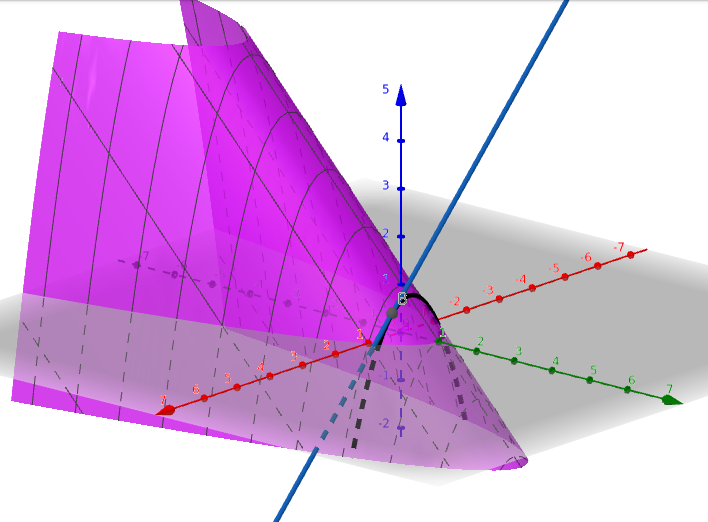
\includegraphics[scale=0.24]{tangent.png};
\qquad
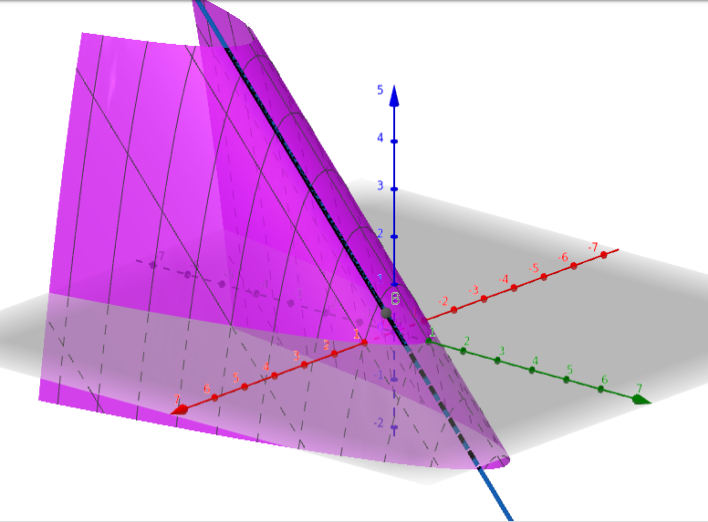
\includegraphics[scale=0.24]{tangent2.png};
\end{figure}
Таких дотичних прямих існують безліч, але про це згодом.
\end{example}


\begin{proposition}[Необхнідна умова диференційованості]
Задано функцію $f: A \to \mathbb{R}$ - диференційована в т. $\vec{x}^0 \in A$ - внутрішня точка. Тоді вона має часткові похідні в т. $\vec{x}^0$, причому $\departial{f}{x_j} (x_1^0,\dots,x_j^0,\dots,x_m^0) = L_j$.
\end{proposition}

\begin{proof}
$f$ - диференційована в т. $\vec{x}^0$, тоді $\exists L_1,\dots,L_m \in \mathbb{R}: \\ f(\vec{x}^0 + \Delta \vec{x}) - f(\vec{x}^0) = L_1 \Delta x_1 + \dots + L_m \Delta x_m + o(\Norm{\Delta \vec{x}}), \Delta \vec{x} \to \vec{0}$.\\
У частному випадку, встановити можна $\Delta \vec{x} = \begin{pmatrix}
0 & \dots & \Delta x_j & \dots & 0
\end{pmatrix}^T$.\\
Тоді $\departial{f}{x_j}(x_1^0,\dots,x_j^0,\dots,x_m^0) = \huge\lim_{\Delta x_j \to 0} \dfrac{f(x_1^0,\dots,x_j^0+\Delta x_j,\dots,x_m^0) - f(x_1^0,\dots,x_j^0,\dots,x_m^0)}{\Delta x_j} \overset{f \text{ - диф.}}{=} \\ = \lim_{\Delta x_j \to 0} \dfrac{L_1 \cdot 0 + \dots + L_j \Delta x_j + \dots + L_m \cdot 0 + o(|\Delta x_j|)}{\Delta x_j} = \lim_{\Delta x_j \to 0} \dfrac{L_j \Delta x_j + o(\Delta x_j)}{\Delta x_j} = L_j$.
\end{proof}

\begin{remark}
У зворотньому напрямку це не завжди вірно.
\end{remark}

\begin{example}
Маємо функцію $f(x,y) = \sqrt{|xy|}$. Розглянемо цю функції в околі т. $(x_0,y_0) = (0,0)$.\\
$\departial{f}{x}(0,0) = \huge\lim_{\Delta x \to 0} \dfrac{f(\Delta x,0) - f(0,0)}{\Delta x} = \lim_{\Delta x \to 0} \dfrac{\sqrt{|\Delta x \cdot 0| - 0}}{\Delta x} = 0$.\\
$\departial{f}{y}(0,0) = \huge\lim_{\Delta y \to 0} \dfrac{f(0,\Delta y) - f(0,0)}{\Delta y} = \lim_{\Delta y \to 0} \dfrac{\sqrt{|0 \cdot \Delta y| - 0}}{\Delta y} = 0$.\\
Тобто в т. $(x_0,y_0)$ функція має часткові похідні. Проте виявляється, що в $(x_0,y_0)$ вона - не диференційована. Дійсно,\\
$f(\Delta x,\Delta y) = 0 \Delta x + 0 \Delta y + o(\sqrt{\Delta x^2 + \Delta y^2}) = o(\sqrt{\Delta x^2 + \Delta y^2})$, тобто\\
$\huge\lim_{\substack{\Delta x \to 0 \\ \Delta y \to 0}} \dfrac{f(\Delta x,\Delta y)}{\sqrt{\Delta x^2 + \Delta y^2}} = \lim_{\substack{\Delta x \to 0 \\ \Delta y \to 0}} \dfrac{\sqrt{|\Delta x \Delta y|}}{\sqrt{\Delta x^2 + \Delta y^2}} \overset{\text{полярна заміна}}{=} \lim_{\rho \to 0} \sqrt{|\cos \varphi \sin \varphi|}$ - не існує, тому рівність вище не вірна.
\begin{figure}[H]
\centering
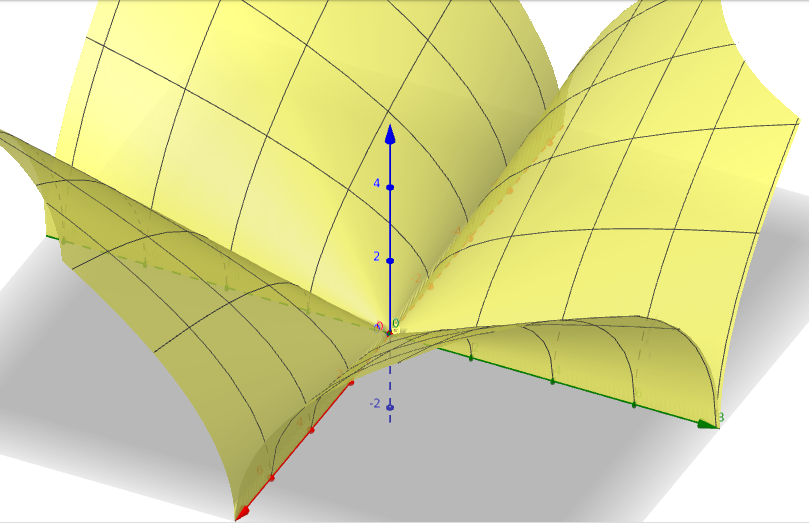
\includegraphics[scale=0.24]{not_differentiable.png}
\end{figure}
Можливо виникне питання, а чи існують інші числа $(L_1,L_2) \neq (0,0)$. Ні. Це випливає з необхідної умови диференційованості.
\end{example}

Виникає тоді інше питання, а коли ми можемо гарантувати диференційованість через існування похідних.

\begin{theorem}[Достатня умова диференційованості]
Задано функцію $f: A \to \mathbb{R}$ та $\vec{x}^0 \in A$ - внутрішня точка.\\
Відомо, що в деякому околі т. $\vec{x}^0$ існують всі часткові похідні в околі т. $\vec{x}^0$, які неперервні в т. $\vec{x}^0$. Тоді $f$ - диференційована в т. $\vec{x}^0$.
\end{theorem}
\begin{proof}
\textit{Ми будемо доводити, коли $m = 2$. Для більших аргументів - аналогічно, але більш технічна справа}
\bigskip \\
Отже, дано $f(x,y)$ та в околі т. $(x_0,y_0)$ існують часткові похідні $\dfrac{\partial f}{\partial x}$ та $\dfrac{\partial f}{\partial y}$, які неперервні в $(x_0,y_0)$.\\
$f(x_0 + \Delta x, y_0 + \Delta y) - f(x_0, y_0) = f(x_0 + \Delta x, y_0 + \Delta y) - \textcolor{red}{f(x_0+\Delta x, y_0)} + \textcolor{red}{f(x_0+\Delta x, y_0)} - f(x_0, y_0) \boxed{=}$\\
Позначу $h(t) = f(x_0+ \Delta x, y_0+t), t \in [0, \Delta y]$. Тоді $f(x_0 + \Delta x, y_0 + \Delta y) - f(x_0+\Delta x, y_0) = h(\Delta y) - h(0)$.\\
$h$ - диференційована на $[0,\Delta y]$, оскільки існує $\departial{f}{y}$, яка неперервна. А тому $h \in C([0,\Delta y])$. Тоді за Лагранжом:\\
$h(\Delta y) - h(0) = h'(c_1) \Delta y, c_1 \in (0,y)$\\
$h'(t) = f'_t(x_0+\Delta x, y_0 + t) = \dfrac{\partial f}{\partial y}(x_0 + \Delta x, y_0 + t)$\\
$\implies h(\Delta y) - h(0) = \dfrac{\partial f}{\partial y}(x_0 + \Delta x, y_0 + c_1) \Delta y$.
\bigskip \\
Аналогічно $g(s) = f(x_0 + s, y_0), s \in [0, \Delta x]$. Тоді $f(x_0+\Delta x, y_0) - f(x_0,y_0) = g(\Delta x) - g(0) \overset{\textrm{Лагранжа}}{=} \\ = g'(c_2) \Delta x = \dfrac{\partial f}{\partial x}(x_0+c_2, y_0) \Delta x, c_2 \in (0, \Delta x)$.\\
Повертаємось до нашої рівності.
\bigskip \\
$\boxed{=} \dfrac{\partial f}{\partial y}(x_0 + \Delta x, y_0 + c_1) \Delta y + \dfrac{\partial f}{\partial x}(x_0+c_2, y_0) \Delta x$\\
Лишилось довести, що\\
$(f(x_0 + \Delta x, y_0 + \Delta y) - f(x_0,y_0)) - \left(\dfrac{\partial f}{\partial x}(x_0,y_0) \Delta x + \dfrac{\partial f}{\partial y}(x_0,y_0) \Delta y \right) = \underset{\Delta x \to 0 \\ \Delta y \to 0}{o(||(\Delta x, \Delta y)||)}$.\\
Маємо:\\
$(f(x_0 + \Delta x, y_0 + \Delta y) - f(x_0,y_0)) - \left(\dfrac{\partial f}{\partial x}(x_0,y_0) \Delta x + \dfrac{\partial f}{\partial y}(x_0,y_0) \Delta y \right) = \\
= \left(\dfrac{\partial f}{\partial y}(x_0 + \Delta x, y_0 + c_1) \Delta y + \dfrac{\partial f}{\partial x}(x_0+c_2, y_0) \Delta x \right) - \left(\dfrac{\partial f}{\partial x}(x_0,y_0) \Delta x + \dfrac{\partial f}{\partial y}(x_0,y_0) \Delta y \right) = \\ = \left(\dfrac{\partial f}{\partial x}(x_0+c_2, y_0) - \dfrac{\partial f}{\partial x}(x_0,y_0) \right) \Delta x + \left(\dfrac{\partial f}{\partial y}(x_0 + \Delta x, y_0 + c_1) - \dfrac{\partial f}{\partial y}(x_0,y_0) \right) \Delta y$\\
Якщо $\Delta x \to 0, \Delta y \to 0$, то звідси $c_1 \to 0, c_2 \to 0$ та за умовою того, що часткові похідні є неперервними, маємо:\\
$\left(\dfrac{\partial f}{\partial x}(x_0+c_2, y_0) - \dfrac{\partial f}{\partial x}(x_0,y_0) \right) \overset{\textrm{позн}}{=} \alpha \to 0$\\
$\left(\dfrac{\partial f}{\partial y}(x_0 + \Delta x, y_0 + c_1) - \dfrac{\partial f}{\partial y}(x_0,y_0) \right) \overset{\textrm{позн}}{=} \beta \to 0$\\
Далі:\\
$\abs{\dfrac{\alpha \Delta x + \beta \Delta y}{\sqrt{\Delta x^2 + \Delta y^2}}} \overset{\textrm{К-Б}}{\leq} \abs{\dfrac{\sqrt{\alpha^2+\beta^2} \sqrt{\Delta x^2 + \Delta y^2}}{\Delta x^2 +\Delta y^2}} \to 0 \implies \dfrac{\alpha \Delta x + \beta \Delta y}{\sqrt{\Delta x^2 + \Delta y^2}} \to 0, \Delta x \to 0, \Delta y \to 0$.\\
Остаточно отримуємо:\\
$(f(x_0 + \Delta x, y_0 + \Delta y) - f(x_0,y_0)) - \left(\dfrac{\partial f}{\partial x}(x_0,y_0) \Delta x + \dfrac{\partial f}{\partial y}(x_0,y_0) \Delta y \right) = \underset{\Delta x \to 0 \\ \Delta y \to 0}{o(||(\Delta x, \Delta y)||)}$.
\end{proof}

\begin{definition}
Задано функцію $f: A \to \mathbb{R}$ та $\vec{x}^0 \in A$ - внутрішня точка.\\
\textbf{Похідною функції} $f$ \textbf{в т.} $\vec{x}^0$ називається ковектор
\begin{align*}
f'(\vec{x}^0) = \begin{pmatrix}
\departial{f}{x_1} & \dots & \departial{f}{x_m}
\end{pmatrix} (\vec{x}^0)
\end{align*}
\end{definition}
Використовуючи нове означення, умова диференційованості перепишеться тоді абсолютно звичним чином:\\
$f(\vec{x}^0 + \Delta \vec{x}) - f(\vec{x}^0) = f'(\vec{x}^0) \cdot \Delta \vec{x} + o(\Norm{\Delta \vec{x}}), \Delta \vec{x} \to \vec{0}$.


\iffalse
\begin{definition}
Задано функцію $f: A \to \mathbb{R}$ та $\vec{x}^0 \in A$ - внутрішня точка.\\
\textbf{Градієнтом функції} $f$ \textbf{в т.} $\vec{x}^0$ називається вектор
\begin{align*}
\grad f(\vec{x}^0) \overset{\textrm{або}}{=} \textrm{grad} f(\vec{x}^0) = \begin{pmatrix}
L_1 \\ \vdots \\ L_m
\end{pmatrix} = \overrightarrow{L}
\end{align*}
\textbf{Похідною функції} $f$ \textbf{в т.} $\vec{x}^0$ називається ковектор
\begin{align*}
f'(\vec{x}^0) = \begin{pmatrix}
L_1 & \dots & L_m
\end{pmatrix} = \overleftarrow{L}
\end{align*}
\end{definition}
У випадку функції від трьох змін $f(x,y,z)$, градієнт можна розписати таким чином:\\
$\textrm{grad} f(x,y,z) = \dfrac{\partial f}{\partial x} \vec{i} + \dfrac{\partial f}{\partial y} \vec{j} + \dfrac{\partial f}{\partial z} \vec{k}$
\bigline

Перепишемо умову диференційованості:\\
$f(\vec{x}^0 + \Delta \vec{x}) - f(\vec{x}^0) = L_1 \Delta x_1 + \dots + L_m \Delta x_m + \underset{\Delta \vec{x} \to 0}{o(||\vec{x}||)} \boxed{=}$\\
Якщо згадати, що $L_1 \Delta x_1 + \dots + L_m \Delta x_m = \left( \overrightarrow{L} \overrightarrow{\Delta x} \right) = \left(\textrm{grad} f(\vec{x}^0), \overrightarrow{\Delta x}\right)$\\
Або побачити, що $L_1 \Delta x_1 + \dots + L_m \Delta x_m = \begin{pmatrix}
L_1 & \dots & L_m
\end{pmatrix} \begin{pmatrix}
\Delta x_1 \\ \vdots \\ \Delta x_m
\end{pmatrix} = f'(\vec{x}^0) \overrightarrow{\Delta x}$\\
Тоді продовжимо рівність\\
$\boxed{=} \left(\textrm{grad} f(\vec{x}^0), \overrightarrow{\Delta x}\right) + \underset{\Delta \vec{x} \to 0}{o(||\vec{x}||)} = f'(\vec{x}^0) \overrightarrow{\Delta x} + \underset{\Delta \vec{x} \to 0}{o(||\vec{x}||)}$
\bigline
\fi

\begin{proposition}
Задані функції $f,g: A \to \mathbb{R}$ та $\vec{x}^0 \in A$ - внутрішня точка. Відомо, що $f,g$ - диференційовані в т. $\vec{x}^0$. Тоді:\\
1) $\alpha f$ - диференційована в т. $\vec{x}^0$, $\forall \alpha \in \mathbb{R}$, похідна $(\alpha f)'(\vec{x}^0) = \alpha f'(\vec{x}^0)$;\\
2) $f + g$ - диференційована в т. $\vec{x}^0$, похідна $(f+g)'(\vec{x}^0) = f'(\vec{x}^0)+g'(\vec{x}^0)$;\\
3) $fg$ - диференційована в т. $\vec{x}^0$, похідна $(fg)'(\vec{x}^0) = f'(\vec{x}^0) g(\vec{x}^0) + f(\vec{x}^0)g'(\vec{x}^0)$.
\end{proposition}

\begin{proof}
1) \textit{Зрозуміло.}
\bigskip \\
2) $(f(\vec{x}^0 + \Delta \vec{x}) + g(\vec{x}^0 + \Delta \vec{x})) - (f(\vec{x}^0) + g(\vec{x}^0)) = (f(\vec{x}^0+\Delta \vec{x}) - f(\vec{x}^0)) + (g(\vec{x}^0+\Delta \vec{x}) - g(\vec{x}^0)) = \\
= f'(\vec{x}^0) \cdot \Delta \vec{x} + o(\Norm{\Delta \vec{x}}) + g'(\vec{x}^0) \cdot \Delta \vec{x} + o(\Norm{\Delta \vec{x}}) = (f'(\vec{x}^0)+g'(\vec{x}^0)) \cdot \Delta \vec{x} + o(\Norm{\Delta \vec{x}}), \Delta \vec{x} \to \vec{0}$.
\bigskip \\
3) $f(\vec{x}^0 + \Delta \vec{x})g(\vec{x}^0 + \Delta \vec{x}) - f(\vec{x}^0) g(\vec{x}^0) = \\
= (f(\vec{x}^0) + f'(\vec{x}^0) \cdot \Delta \vec{x} + o(\Norm{\Delta \vec{x}}))\cdot(g(\vec{x}^0) + g'(\vec{x}^0) \cdot \Delta \vec{x} + o(\Norm{\Delta \vec{x}})) - f(\vec{x}^0)g(\vec{x}^0) \boxed{=}$\\
Після розкриття дужок ми залишимо лише доданки $(f(\vec{x}^0) g'(\vec{x}^0)) \cdot \Delta \vec{x}$ та $(g(\vec{x}^0) f'(\vec{x}^0)) \cdot \Delta \vec{x}$. \\
Ось чому:\\
$f(\vec{x}^0) o(\Norm{\Delta \vec{x}}) = o(\Norm{\Delta \vec{x}})$ \hspace{1cm} $g(\vec{x}^0) o(\Norm{\Delta \vec{x}}) = o(\Norm{\Delta \vec{x}})$\\
$(f'(\vec{x}^0) \cdot \Delta \vec{x}) \cdot (g'(\vec{x}^0) \cdot \Delta \vec{x}) = o(\Norm{\Delta \vec{x}})$, тому що, розписавши, побачимо, що $\Delta x_i \Delta x_j = o(\Norm{\Delta \vec{x}})$ (зрозуміло)\\
$(f'(\vec{x}^0) \cdot \Delta \vec{x}) o(\Norm{\Delta \vec{x}}) = o(\Norm{\Delta \vec{x}})$ \hspace{1cm} $(g'(\vec{x}^0) \cdot \Delta \vec{x}) o(\Norm{\Delta \vec{x}}) = o(\Norm{\Delta \vec{x}})$ \hspace{1cm}, тому що, розписавши, побачимо $\Delta x_j o(\Norm{\Delta \vec{x}}) = o(\Norm{\Delta \vec{x}})$\\
$(o(\Norm{\Delta \vec{x}}))^2 = o(\Norm{\Delta \vec{x}})$\\
Повертаємось до рівності:\\
$\boxed{=} (f(\vec{x}^0)g'(\vec{x}^0)) \cdot \Delta \vec{x} + (g(\vec{x}^0) f'(\vec{x}^0)) \cdot \Delta \vec{x} + o(\Norm{\Delta \vec{x}})$.
\end{proof}

\begin{definition}
Задано функцію $f: A \to \mathbb{R}$ та $\vec{x}^0 \in A$ - внутрішня точка.\\
\textbf{Диференціалом функції} $f(x)$ \textbf{в т.} $\vec{x}^0$ називається такий вираз:
\begin{align*}
df(\vec{x}^0, \Delta \vec{x}) = f'(\vec{x}^0) \cdot \Delta \vec{x}
\end{align*}
\end{definition}

Як й раніше, аргумент $\Delta \vec{x}$ опускають, а також позначають $\Delta \vec{x}= \vec{dx}$, тобто \\ $\Delta x_1 = dx_1, \dots, \Delta x_m = dx_m$. Тоді маємо інший вигляд:
\begin{align*}
df(\vec{x}^0) = f'(\vec{x}^0) \cdot \vec{dx} = \departial{f}{x_1}(\vec{x}^0)\,dx_1 + \dots + \departial{f}{x_m}(\vec{x}^0)\,dx_m
\end{align*}

\begin{example}
Маємо функцію $f(x,y) = 1-x^2 - y$. Ми вже знайшли $\departial{f}{x} = -2x, \departial{f}{y} = -1$, вони є неперервними в будь-якій точці.\\
Отже, $f$ - диференційована будь-де. Знадемо тепер диференціал функції. Це дуже просто:\\
$d f(x,y) = \departial{f}{x}\,dx + \departial{f}{y}\,dy = (-2x)\,dx -\,dy \overset{\text{або}}{=} \begin{pmatrix}
-2x & -1
\end{pmatrix} \, \vec{dr}$.
\end{example}

\subsection{Для векторнозначних функцій}
\begin{definition}
Задано функцію $\vec{f}: A \to \mathbb{R}^k$ та $\vec{x}^0 \in A$ - внутрішня точка.\\
Вектор-функція $\vec{f}$ називається \textbf{диференційованою в т.} $\vec{x}^0$, якщо
\begin{align*}
\exists M \in Mat(m \times k): \vec{f}(\vec{x}^0 + \Delta \vec{x}) - \vec{f}(\vec{x}^0) = M \Delta \vec{x} + \underset{\Delta \vec{x} \to \vec{0}}{\vec{o}(||\Delta \vec{x}||)}
\end{align*}
\end{definition}
Зараз дізнаємось, що це за матриця $M = \begin{pmatrix}
M_{11} & \dots & M_{1m} \\
\vdots & \ddots & \vdots \\
M_{k1} & \dots & M_{km}
\end{pmatrix}$ під час доведення твердження.

\begin{proposition}
Задано функцію $\vec{f}: A \to \mathbb{R}^k$ та $\vec{x}^0 \in A$ - внутрішня точка.\\
$\vec{f}$ - диференційована в т. $\vec{x}^0 \iff f_1,\dots,f_k$ - диференційовані в т. $\vec{x}^0$.
\end{proposition}

\begin{proof}
\rightproof Дано: $\vec{f}$ - диференційована в т. $\vec{x}^0$, тобто $\exists M \in Mat(m \times k): \vec{f}(\vec{x}^0 + \Delta \vec{x}) - \vec{f}(\vec{x}^0) = M \Delta \vec{x} + \underset{\Delta \vec{x} \to \vec{0}}{\vec{o}(||\Delta \vec{x}||)}$.\\
$\begin{pmatrix}
f_1(\vec{x}^0 + \Delta \vec{x}) \\ \vdots \\ f_k(\vec{x}^0 + \Delta \vec{x})
\end{pmatrix} - \begin{pmatrix}
f_1(\vec{x}^0) \\ \vdots \\ f_k(\vec{x}^0)
\end{pmatrix} = \begin{pmatrix}
M_{11} & \dots & M_{1m} \\
\vdots & \ddots & \vdots \\
M_{k1} & \dots & M_{km}
\end{pmatrix} \begin{pmatrix}
\Delta x_1 \\ \vdots \\ \Delta x_m
\end{pmatrix} + \begin{pmatrix}
o(||\Delta \vec{x}||) \\ \vdots \\ \vec{o}(||\Delta \vec{x}||)
\end{pmatrix}$\\
Із цієї рівності випливає, що $\forall j = \overline{1,k}:$\\
$f_j(\vec{x}^0 + \Delta \vec{x}) - f_j(\vec{x}^0) = M_{j1} \Delta x_1 + \dots + M_{jm} \Delta x_m + \underset{\Delta \vec{x} \to 0}{o(||\Delta \vec{x}||)}$.\\
Це означає, що $f_j$ - диференційована в т. $\vec{x}^0$. Тоді звідси випливає, що:\\
$M_{j1} = \dfrac{\partial f_j}{\partial x_1} (\vec{x}^0), \dots, M_{jm} = \dfrac{\partial f_j}{\partial x_m} (\vec{x}^0)$.\\
В результаті отримаємо ось такий вигляд матриці:\\
$M = \begin{pmatrix}
\dfrac{\partial f_1}{\partial x_1} & \dots & \dfrac{\partial f_1}{\partial x_m} \\
\vdots & \ddots & \vdots \\
\dfrac{\partial f_k}{\partial x_1} & \dots & \dfrac{\partial f_k}{\partial x_m}
\end{pmatrix}(\vec{x}^0) = \begin{pmatrix}
f'_1 \\ \vdots \\ f_k'
\end{pmatrix}(\vec{x}^0) = J(x) = \vec{f}'(\vec{x}^0)$ - \textbf{матриця Якобі}\\
Матриця Якобі описує \textbf{похідну} вектор-функції $\vec{f}$ в т. $\vec{x}^0$. А якщо матриця буде квадратною, то ми можемо обчислити $\det \vec{f}'(\vec{x}^0)$ - \textbf{якобіан}.
\bigskip \\
\leftproof Дано: $f_1,\dots,f_k$ - диференційовані в т. $\vec{x}^0$. Хочемо довести, що \\
$\vec{f}(\vec{x}^0+\Delta \vec{x}^0) - \vec{f}(\vec{x}^0) - M\Delta \vec{x} = \vec{o}(\Norm{\Delta \vec{x}}), \Delta \vec{x} \to \vec{0}$, але це є правда, тому що:\\
$\forall j = \overline{1,k}: f_j$ - диференційована $\implies f_j(\vec{x}^0+\Delta \vec{x}^0) - f_j(\vec{x}^0) - f_j'(\vec{x}^0) \cdot \Delta \vec{x} = o(\Norm{\Delta \vec{x}}), \Delta \vec{x} \to \vec{0}$ - виконана покоординатна рівність.
\end{proof}

\begin{proposition}
Задано функцію $\vec{f}: A \to \mathbb{R}^k$ та $\vec{x}^0 \in A$ - внутрішня точка.\\
Відомо, що вектор-функція $\vec{f}$ - диференційована в т. $\vec{x}^0$. Тоді вона неперервна в т. $\vec{x}^0$.
\end{proposition}
\begin{proof}
Дійсно, $\huge \lim_{\vec{x} \to \vec{x}^0} \left(M(\vec{x}- \vec{x}^0) + \vec{o}(||\vec{x} - \vec{x}^0||) \right) = 0$, оскільки виконується покоординатна границя.
\end{proof}

\begin{proposition}
Задані функції $\vec{f}, \vec{g}: A \to \mathbb{R}^k$ та $\vec{x}^0 \in A$ - внутрішня точка. Відомо, що $\vec{f},\vec{g}$ - диференційовані в т. $\vec{x}^0$.\\
Тоді $\alpha \vec{f} + \beta \vec{g}$ - диференційована в т. $\vec{x}^0$, похідна $(\alpha \vec{f} + \beta \vec{g})'(\vec{x}^0) = \alpha \vec{f}'(\vec{x}^0) + \beta \vec{g}'(\vec{x}^0)$.\\
\textit{Випливає з арифметики матриці. Ну тут зрозуміло.}
\end{proposition}

\begin{example}[Важливий]
Маємо вектор-функцію $\begin{pmatrix}
x \\ y
\end{pmatrix} = \begin{pmatrix}
\rho \cos \varphi \\
\rho \sin \varphi
\end{pmatrix}$. Знайдемо її похідну та якобіан.\\
$\vec{f}'(\vec{x}^0) = \begin{pmatrix}
\departial{x}{\rho} & \departial{x}{\varphi} \\
\departial{y}{\rho} & \departial{y}{\varphi}
\end{pmatrix} = \begin{pmatrix}
\cos \varphi & -\rho \sin \varphi \\
\sin \varphi & \rho \cos \varphi
\end{pmatrix}$ \hspace{1cm} $\det \vec{f}'(\vec{x}^0) = \cos \varphi \rho \cos \varphi + \sin \varphi \rho \sin \varphi = \rho$.\\
Ще знадобиться, коли будемо шукати подвійні інтеграли.
\end{example}

\begin{proposition}
Задані функції $\vec{f}: A \to B$ та $\vec{g}: B \to \mathbb{R}^k$, де $A \subset \mathbb{R}^m, B \subset \mathbb{R}^n$.\\
Відомо, що $\vec{f}$ - диференційована в т. $\vec{x}^0$ та $\vec{g}$ - диференційована в т. $\vec{y}^0$. \\ Тоді $\vec{g} \circ \vec{f}$ - диференційована в т. $\vec{x}^0$, похідна $(\vec{g} \circ \vec{f})'(\vec{x}^0) = \vec{g}'(\vec{y}^0) \vec{f}'(\vec{x}^0)$.
\end{proposition}

\iffalse
\begin{lemma}
Задано матрицю $A \in Mat(m \times k)$. Тоді $\exists C \geq 0: \forall \vec{h} \in \mathbb{R}^m: \Norm{A \vec{h}} \leq C \Norm{\vec{h}}$.
\end{lemma}

\begin{proof}
Дійсно, $A = \begin{pmatrix}
a_{11} & \dots & a_{1m} \\
\vdots & \ddots & \vdots \\
a_{k1} & \dots & a_{km}
\end{pmatrix} \implies A \vec{h} = \begin{pmatrix}
a_{11}h_1 + \dots + a_{1m} h_m \\
\vdots \\
a_{k1}h_1 + \dots + a_{km} h_m
\end{pmatrix}$\\
$\implies \Norm{A \vec{h}} = \sqrt{(a_{11}h_1+\dots+a_{1m}h_m)^2 + \dots + (a_{k1}h_1+\dots+a_{km}h_m)^2} \overset{\text{К-Б}}{\leq} \\ \leq \sqrt{(a_{11}^2+\dots+a_{1m}^2)(h_1^2+\dots+h_m^2) + \dots + (a_{k1}^2+\dots+a_{km}^2)(h_1^2+\dots+h_m^2)} = \\ = \Norm{\vec{h}}\sqrt{(a_{11}^2+\dots+a_{1m}^2)+ \dots + (a_{k1}^2+\dots+a_{km}^2)} = C \Norm{\vec{h}}$.
\end{proof}
Тепер безпосередньо доведення твердження.
\fi

\begin{proof}
$\vec{g} \circ \vec{f} (\vec{x}^0 + \Delta \vec{x}) - \vec{g} \circ \vec{f} (\vec{x}^0) = \vec{g}(\vec{f}(\vec{x}^0+\Delta \vec{x})) - \vec{g}(\vec{f}(\vec{x}^0)) = \vec{g}(\vec{f}(\vec{x}^0) + \vec{f}'(\vec{x}^0) \Delta \vec{x} + \vec{o}(\Norm{\Delta \vec{x}})) - \vec{g}(\vec{f}(\vec{x}^0)) = \\
= \vec{g}(\vec{y}^0 + \Delta \vec{y}) - \vec{g}(\vec{y}^0) = \vec{g}'(\vec{y}^0) \Delta \vec{y} + o(\Norm{\Delta \vec{y}}) = \vec{g}'(\vec{y}^0) \vec{f}'(\vec{x}^0) \Delta \vec{x} + \vec{g}'(\vec{y}^0) \vec{o}(\Norm{\Delta \vec{x}}) + \vec{o}(\Norm{\Delta \vec{y}}) \boxed{=}$\\
Лишилось довести, що $\vec{g}'(\vec{y}^0) \vec{o}(\Norm{\Delta \vec{x}}) + \vec{o}(\Norm{\Delta \vec{y}}) = \vec{o}(\Norm{\Delta \vec{x}})$, якщо $\Delta \vec{x} \to \vec{0}$, але тут зрозуміло.\\
$\boxed{=} \vec{g}'(\vec{y}^0) \vec{f}'(\vec{x}^0) \Delta \vec{x} + \vec{o}(\Norm{\Delta \vec{x}})$.
\end{proof}

\begin{corollary}
Задано функцію $\vec{f}: A \to B$ та $g: B \to \mathbb{R}$, де $A \subset \mathbb{R}^m, B \subset \mathbb{R}^n$.\\
Відомо, що $\vec{f}$ - диференційована в т. $\vec{x}^0$ та $g$ - диференційована в т. $\vec{y}^0$.\\
Тоді $\departial{h}{x_j}(\vec{x}^0) = \departial{g}{y_1}(\vec{y}^0) \departial{f_1}{x_j}(\vec{x}^0) + \departial{g}{y_2}(\vec{y}^0) \departial{f_2}{x_j}(\vec{x}^0) + \dots + \departial{g}{y_n}(\vec{y}^0) \departial{f_n}{x_j}(\vec{x}^0)$, виконано $\forall j = \overline{1,m}$.
\end{corollary}

\begin{example}
Маємо функцію $f\left( xy, \dfrac{x}{y} \right)$. Знайдемо часткові похідні за $x,y$.\\
Позначимо $u(x,y) = xy$, $v(x,y) = \dfrac{x}{y}$. Тоді маємо:\\
$\departial{f}{x} = \departial{f}{u} \departial{u}{x} + \departial{f}{v} \departial{v}{x} = \departial{f}{u} \cdot y + \departial{f}{v} \cdot \dfrac{1}{y}$\\
$\departial{f}{y} = \departial{f}{u} \departial{u}{y} + \departial{f}{v} \departial{v}{y} = \departial{f}{u} \cdot x + \departial{f}{v} \cdot \dfrac{-x}{y^2}$
\end{example}

\subsection{Похідна за напрямком. Градієнт}
\begin{definition}
Задано функцію $f: A \to \mathbb{R}$ та $\vec{x}^0 \in A$ - внутрішня точка. А також задано вектор $\vec{l}$, такий, що $\Norm{\vec{l}} = 1$. Її ще називають \textbf{напрямком}.\\
\textbf{Похідною функції} $f$ \textbf{за напрямком} $\vec{l}$ \textbf{в т. $\vec{x}^0$} називають величину
\begin{align*}
\dfrac{\partial f}{\partial \vec{l}} (\vec{x}^0) = \lim_{t \to 0} \dfrac{f(\vec{x}^0+t \vec{l}) - f(\vec{x}^0)}{t}
\end{align*}
Як вже було зазначено, дотичних прямих буває дуже багато, тому ми й задаємо напрямок.
\end{definition}

\begin{remark}
Якщо всі координати вектора $\vec{l}$ будуть нулевими, окрім $l_j = 1$, то $\dfrac{\partial f}{\partial \vec{l}} (\vec{x}^0) = \dfrac{\partial f}{\partial x_j} (\vec{x}^0)$.
\end{remark}

\begin{theorem}
Задано функцію $f$ - диференційована в т. $\vec{x}^0 \in A$ - внутрішня точка. Тоді\\
$\departial{f}{\vec{l}}(\vec{x}^0) = f'(\vec{x}^0) \cdot \vec{l} = \departial{f}{x_1} l_1 + \dots + \departial{f}{x_m} l_m$.
\end{theorem}

\begin{proof}
$f$ - диференційована в т. $\vec{x}^0$, тобто $f(\vec{x}^0 + t \vec{l}) - f(\vec{x}^0) = \departial{f}{x_1}tl_1 + \dots + \departial{f}{x_m}tl_m + o(\Norm{t\vec{l}})$.\\
Тому $\departial{f}{\vec{l}}(\vec{x}^0) = \huge\lim_{t \to 0} \dfrac{f(\vec{x}^0+t\vec{l}) - f(\vec{x}^0)}{t} = \lim_{t \to 0} \dfrac{\departial{f}{x_1}tl_1 + \dots + \departial{f}{x_m}tl_m + o(\Norm{t\vec{l}})}{t} = \departial{f}{x_1}l_1 + \dots + \departial{f}{x_m}l_m$.
\end{proof}

\begin{example}
Маємо функцію $f(x,y) = 1 - x^2 - y$. Знайти похідну за напрямком $\vec{l} = (0.6,0.8)$.\\
$\departial{f}{x} = -2x \hspace{1cm} \departial{f}{y} = -1$.\\
$\implies \departial{f}{\vec{l}} = -0.6 \cdot 2x -0.8 \cdot 1 = -1.2x - 0.8$.
\end{example}

\begin{definition}
Задано функцію $f: A \to \mathbb{R}$ та $\vec{x}^0 \in A$ - внутрішня точка.\\
\textbf{Градієнтом функції} $f$ \textbf{в т.} $\vec{x}^0$ називають такий вектор
\begin{align*}
\wordgrad f(\vec{x}^0) \overset{\text{або}}{=} \grad f(\vec{x}^0) = \begin{pmatrix}
\departial{f}{x_1} \\ \vdots \\ \departial{f}{x_m}
\end{pmatrix}(\vec{x}^0)
\end{align*}
\end{definition}

Похідну функції $\vec{f}$ за напрямком $\vec{l}$ в т. $\vec{x}^0$ можна записати інакше:\\
$\departial{f}{\vec{l}} = \left( \wordgrad f(\vec{x}^0), \vec{l} \right)$.


\begin{proposition}
$\dfrac{\partial f}{\partial \vec{l}}(\vec{x}^0)$ приймає:\\
- max значення $ \iff \vec{l} \uparrow \uparrow \textrm{grad} \vec{f}(\vec{x}^0)$;\\
- min значення,$ \iff \vec{l} \uparrow \downarrow \textrm{grad} \vec{f}(\vec{x}^0)$.
\end{proposition}

\begin{proof}
Дійсно, $\departial{f}{\vec{l}}(\vec{x}^0) = \left( \wordgrad f(\vec{x}^0), \vec{l} \right) = \Norm{\wordgrad f(\vec{x}^0)} \Norm{\vec{l}} \cos \alpha = \Norm{\wordgrad f(\vec{x}^0)} \cos \alpha$:\\
- max $\iff \alpha = 0$;\\
- min $\iff \alpha = \pi$.
\end{proof}

\subsection{Неявно задані функції}
\begin{remark}[Приклад для розуміння]
Задано рівняння кола на площині $\mathbb{R}^2$ - один з прикладів неявної функції:\\ $x^2+y^2-1=0$.
\begin{figure}[H]
\centering
\begin{tikzpicture}
\draw[thick,->] (-2.2,0)--(2.5,0) node[anchor = north west] {$x$};
\draw[thick,->] (0,-2.2)--(0,2.5) node[anchor = south east] {$y$};
\draw (0,0) circle (2);
\node at(2.2,-0.2) {$1$};
\end{tikzpicture}
\end{figure}
Зрозуміло, що це - не графік функції однієї змінної. Просто тому що кожному значенню $x$ тут ставиться у відповідність два значення $y$.\\
Проте якщо розглядати деякий малий окіл т. $(x_0,y_0)$, то ми отримаємо деякий шматок малюнку, що й буде графіком функції. Зокрема в нашому випадку або $y = \sqrt{1-x^2}$, або $y = -\sqrt{1-x^2}$.\\
Проте існують певні точки, де цього зробити не можна - точки $(1,0),(-1,0)$. Як би ми не зменшували окіл цієї точки, там завжди кожного іксу два ігрика були б. Я цю точку позначил червоним кольором.
\begin{figure}[H]
\centering
\begin{tikzpicture}
\draw[thick,->] (-2.2,0)--(2.5,0) node[anchor = north west] {$x$};
\draw[thick,->] (0,-2.2)--(0,2.5) node[anchor = south east] {$y$};
\fill (1,{sqrt(3)}) circle(1.5pt);
\draw[dashed] (1,{sqrt(3)}) circle (0.5);
\fill ({-sqrt(2)},{-sqrt(2)}) circle(1.5pt);
\draw[dashed] ({-sqrt(2)},{-sqrt(2)}) circle (0.5);
\fill[red] (2,0) circle(1.5pt);
\draw[red, dashed] (2,0) circle (0.2);
\draw (0,0) circle (2);
\node at(2.2,-0.2) {$1$};
\end{tikzpicture}
\end{figure}
Саме тому з'явилась мотивацію створити теорему, де через рівняння $F(x,y) = 0$ ми можемо отримати $y = f(x)$ в деякому околі т. $(x_0,y_0)$ під деякими важливими умовами.
\bigskip \\
Важливо розуміти, що функція існує, проте явну формулу отримати не завжди вийде. Зокрема маємо неявну функцію $y^5+y^3+y+x=0$. Щоб знати $y=f(x)$, треба розв'язати рівняння п'ятої степені, проте корені цього многочлена не можна виразити через формулу. І тим не менш, під деякими умовами, ми можемо знати функцію $y=f(x)$, просто без формули.
\end{remark}

\begin{theorem}
Задано неявну функцію $F$ - неперервно-диференційована в околі т. $(x_0,y_0)$. Відомо, що виконуються такі умови:\\
1) $F(x_0,y_0)=0$;\\
2) $\departial{F}{y}(x_0,y_0) \neq 0$.\\
Тоді існує єдина функція $f$ - неперервно-диференційована в меншому околі т. $x_0$, причому $F(x,y) = 0 \iff y = f(x)$, а також $f'(x) = -\dfrac{\departial{F}{x}(x,y) \Big|_{(x,f(x))}}{\departial{F}{y}(x,y) \Big|_{(x,f(x))}}$.
\bigskip \\
Додатково, якщо $F \in C^{(m)}$, то $f \in C^{(m)}$.
\iffalse
Тоді справедливо наступне:\\
I) $\exists \delta_1,\delta_2 > 0: (x_0-\delta_1,x_0+\delta_1) \times (y_0-\delta_2,y_0+\delta_2) \subset U(x_0,y_0)$\\
II) $\exists f: (x_0-\delta_1,x_0+\delta_1) \to (y_0-\delta_2,y_0+\delta_2)$, така, що \\ $f \in C^{(m)}((x_0-\delta_1,x_0+\delta_1))$ та\\
$(x,y) \in (x_0-\delta_1,x_0+\delta_1) \times (y_0-\delta_2,y_0+\delta_2) \iff \begin{cases} x \in (x_0-\delta_1,x_0+\delta_1) \\ y \in (y_0-\delta_2,y_0+\delta_2) \end{cases}$\\
III) $F(x,y) = 0 \iff y=f(x)$\\
IV) $f'(x) = -\dfrac{\departial{F}{x}(x,y) \Big|_{(x,f(x))}}{\departial{F}{y}(x,y) \Big|_{(x,f(x))}}$\\
\textit{Без доведення. Можна подивитись у Зоріча зі 20 сторінками}
\fi
\end{theorem}

\begin{example}
Зокрема для $F(x,y) = x^2+y^2-1$ маємо, що вона - неперервна,\\
$\departial{F}{x} = 2x \hspace{1cm} \departial{F}{y} = 2y$ - диференційована.\\
Причому $\departial{F}{y} \neq 0 \iff y \neq 0$.\\
Тому за попередньою теоремою, дійсно, існує функція $y = f(x)$, але найголовніше: $f'(x) = -\dfrac{x}{y}$.
\end{example}

\begin{theorem}
Задано неявну вектор-функцію $\vec{F}$ - неперервно-диференційована в околі т. $(\vec{x}^0, \vec{y}^0) \in \mathbb{R}^{m+k}$. Відомо, що виконуються такі умови:\\
1) $\vec{F}(\vec{x}^0,\vec{y}^0) = \vec{0}$;\\
2) $\det \vec{F}'_y (\vec{x}^0,\vec{y}^0) \neq 0$. Інакше кажучи, існує оборотна матриця.\\
Тоді існує єдина вектор-функція $\vec{f}$ - неперервно-диференційована в меншому околі т. $\vec{x}^0$, причому $\vec{F}(\vec{x},\vec{y}) = 0 \iff \vec{y} = \vec{f}(\vec{x})$, а також $\vec{f}'(\vec{x}) = -(F'_y(\vec{x},\vec{y}))^{-1} \cdot F'_x (\vec{x},\vec{y}) \Big|_{(\vec{x}, \vec{f}(\vec{x}))}$.\\
\textit{Без доведення.}
\end{theorem}

\begin{example}
Задано вектор-функцію $\vec{F}$ таким чином: $\begin{cases}
x^2+y_1^2 - \dfrac{1}{2}y_2^2 = F_1(x,y_1,y_2) = 0 \\
x+y_1+y_2-2 = F_2(x,y_1,y_2) = 0
\end{cases}$.\\
Маємо $\det \vec{F}'_y(x,y_1,y_2) = \det \begin{pmatrix}
\departial{F_1}{y_1} & \departial{F_1}{y_2} \\
\departial{F_2}{y_1} & \departial{F_2}{y_2} 
\end{pmatrix} = \det \begin{pmatrix}
2y_1 & -y_2 \\
1 & 1
\end{pmatrix} = 2y_1 + y_2 \neq 0 \iff y_2 \neq -2y_1$, а тому й $x \neq 2+y_2$.\\
Тоді враховуючи обмеження, існує вектор-функція $\vec{f}(\vec{x}) = \vec{y}$, але тепер знайдемо похідну. Маємо: \\
$\vec{F}_y' = \begin{pmatrix}
2y_1 & -y_2 \\
1 & 1
\end{pmatrix} \implies (\vec{F}_y')^{-1} = \dfrac{1}{2y_1+y_2} \begin{pmatrix}
1 & y_2 \\
-1 & 2y_1
\end{pmatrix}$\\
$\vec{F}_x' = \begin{pmatrix}
2x \\ 1
\end{pmatrix}$\\
$\vec{f}' = -(\vec{F}'_y)^{-1} \vec{F}'_x = \dfrac{1}{2y_1+y_2} \begin{pmatrix}
1 & y_2 \\
-1 & 2y_1
\end{pmatrix} \begin{pmatrix}
2x \\ 1
\end{pmatrix} = \dfrac{1}{2y_1+y_2} \begin{pmatrix}
2x + y_2 \\ -2x + 2y_1
\end{pmatrix} = \begin{pmatrix}
\dfrac{2x+y_2}{2y_1+y_2} \\ \dfrac{-2x+2y_1}{2y_1+y_2}
\end{pmatrix}$.
\end{example}

\subsection{Обернені функції}
\begin{theorem}
Задано вектор-функцію $\vec{g}: U(\vec{y}^0) \to U(\vec{x}^0)$, де $\vec{x}^0 = \vec{g}(\vec{y}^0)$. Відомо, що виконуються такі умови:\\
1) $\vec{g}$ - неперервно диференційована; \\
2) $\det \vec{g}'(\vec{y}^0) \neq 0$.\\
Тоді існує вектор-функція $\vec{f}: U(\vec{x}^0) \to U(\vec{y}^0)$, причому:\\
1) $\vec{f}$ - неперервно диференційована; \\
2) $\vec{f}'(\vec{x}) = \vec{g}'(\vec{f}(\vec{x}))^{-1}$.\\
\textit{Вказівка: розглянути функцію $\vec{F}(\vec{x},\vec{y}) = \vec{x} - \vec{g}(\vec{y}) = \vec{0}$ та застосувати теорему про неявну вектор-функцію.}
\end{theorem}

\subsection{Геометричне та алгебраїчне застосування}
\subsubsection{Дотична площина, нормальна пряма поверхі}
Задамо функцію $f: A \to \mathbb{R}$ та $\vec{x}^0 \in A \subset \mathbb{R}^2$ - внутрішня точка. Встановимо таку поверхню:
\begin{align*}
\Pi = \{(x,y,z): z = f(x,y) \}
\end{align*}
Площина в $\mathbb{R}^{3}$, що проходить через т. $(x_0, y_0, z_0)$, $z_0 = f(x_0,y_0)$, задається таким рівнянням:
\begin{align*}
z = z_0 + K_1(x-x_0) + K_2(y-y_0) \hspace{1cm} K_1,K_2 \in \mathbb{R}
\end{align*}

\begin{definition}
\textbf{Дотичною площиною} до поверхні $\Pi$ в т. $(x_0,y_0)$ називається площина в $\mathbb{R}^{3}$, що проходить через т. $(x_0,y_0,z_0)$, для якої виконана рівність
\begin{align*}
z - f(x,y) = o(\Norm{(x-x_0,y-y_0)}), (x,y) \to (x_0,y_0)
\end{align*}
\end{definition}

\begin{theorem}
Поверхня $\Pi$ має дотичну площину в т. $(x_0,y_0) \iff f$ - диференційована в т. $(x_0,y_0)$. Причому $K_1 = \departial{f}{x}(x_0,y_0),K_2 = \departial{f}{y}(x_0,y_0)$.\\
\textit{Доведення аналогічне, як в матані $\mathbb{R}$.}
\end{theorem}

Тоді дотична площина задається таким рівнянням:
\begin{align*}
z - f(x_0,y_0) = \departial{f}{x}(x_0,y_0) (x-x_0) + \departial{f}{y}(x_0,y_0) (y-y_0)
\end{align*}

\begin{definition}
\textbf{Нормальною прямою} до поверхні $\Pi$ в т. $(x_0,y_0)$ називається пряма в просторі, що проходить через т. $(x_0,y_0,z_0), z_0 = f(x_0,y_0)$ та перпендикулярна до дотичної площини.
\end{definition}

Вектор нормалі дотичної площини $\vec{N} = \left( \departial{f}{x}(x_0,y_0), \departial{f}{y}(x_0,y_0), -1 \right)$. Це буде напрямним вектором для нормалі прямої. Тоді нормальна пряма задається таким рівнянням:
\begin{align*}
\dfrac{x-x_0}{\departial{f}{x}(x_0,y_0)} = \dfrac{y-y_0}{\departial{f}{y}(x_0,y_0)} = \dfrac{z-z_0}{-1}
\end{align*}

\begin{example}
Задамо функцію $f(x) = x^2+y^2$. Знайдемо дотичну площину та нормальну пряму в т. $(1,-1)$.\\
$f(1,-1) = 2$.\\
$\departial{f}{x}(1,-1) = 2x \Big|_{(1,-1)} = 2$ \hspace{1cm} $\departial{f}{x}(1,-1) = 2y \Big|_{(1,-1)} = -2$.\\
Всі часткові похідні в околі т. $(1,-1)$ неперервні, а тому диференційовані. Отже, можемо отримати дотичну:\\
$z - 2 = 2(x-1) -2(y+1) \implies 2x-2y-z=2$;\\
та нормаль:\\
$\dfrac{x-1}{2} = \dfrac{y+1}{-2} = \dfrac{z-2}{-1}$.
\begin{figure}[H]
\centering
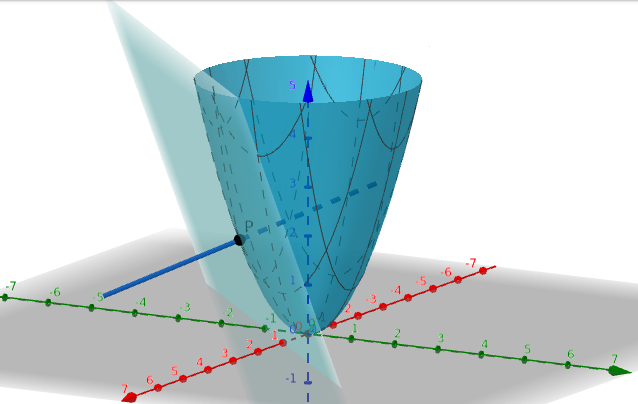
\includegraphics[scale=0.4]{tangent_plane.png}
\end{figure}
\end{example}

\subsubsection{Дотична пряма, нормальна площина кривої}
\begin{definition}
\textbf{Крива} в просторі $\mathbb{R}^3$ задається таким рівнянням
\begin{align*}
\begin{cases} x = x(t) \\ y = y(t) \\ z = z(t) \end{cases} t \in (a,b)
\end{align*}
\textbf{Прямою} в просторі $\mathbb{R}^3$ задається таким рівнянням
\begin{align*}
\begin{cases}
x = s l_1 + x_0, l_1 \in \mathbb{R} \\
y = s l_2 + y_0, l_2 \in \mathbb{R} \\
z = s l_3 + z_0, l_3 \in \mathbb{R}
\end{cases}
\end{align*}
\end{definition}

\begin{definition}
\textbf{Дотичною} прямою до кривої $\vec{x} = \vec{x}(t)$ називається пряма в просторі, що проходить через т. $(x_0,y_0,z_0)$, для якої виконана рівність
\begin{align*}
\begin{cases}
x(t) - (x_0 + l_1(t-t_0)) = o(t-t_0) \\
y(t) - (y_0 + l_2(t-t_0)) = o(t-t_0) \\
z(t) - (z_0 + l_3(t-t_0)) = o(t-t_0)
\end{cases}
\end{align*}
\end{definition}

\begin{theorem}
Пряма $\begin{cases} x = sl_1 + x_0 \\ y = sl_2 + y_0 \\ z = sl_3 + z_0 \end{cases}$ - дотична до кривої $\begin{cases} x = x(t) \\ y = y(t) \\ z = z(t) \end{cases} \iff$ крива - диференційована в т. $t_0$, а також $l_1 = x'(t_0), l_2 = y'(t_0), l_3 = z'(t_0)$.\\
\textit{Вправа: довести}
\end{theorem}
Тоді дотична пряма задається рівнянням:
\begin{align*}
\begin{cases}
x=s x'(t_0)+x_0 \\
y=s y'(t_0)+y_0\\
z=s z'(t_0)+z_0
\end{cases}, s \in \mathbb{R}
\end{align*}
Напрямний вектор прямої $\vec{l} = (x'(t_0),y'(t_0),z'(t_0))$. Тоді це буде нормальним вектором для нормальної плоищини. Нормальна площина задається таким рівнянням:
\begin{align*}
x'(t_0)(x-x_0) + y'(t_0)(y-y_0) + z'(t_0)(z-z_0) = 0
\end{align*}

\begin{example}
Маємо криву $\begin{cases} x = 2 \sin t \\ y = 2 \cos t \\ z = -\sin 2t \end{cases}$, де параметр $t \in [0,2\pi]$. Знайдемо дотичну пряму та нормальну площину в $t_0 = \dfrac{5 \pi}{6}$. Тобто в т. $\left(-1,\sqrt{3}, \dfrac{\sqrt{3}}{2} \right)$.\\
$\begin{cases}
x'(t_0) = 2 \cos t \Big|_{t = t_0} = \sqrt{3} \\
y'(t_0) = -2 \sin t \Big|_{t = t_0} = 1 \\
z'(t_0) = -2 \cos 2t \Big|_{t = t_0} = -1
\end{cases}$.\\
Таким чином, маємо дотичну пряму:\\
$\dfrac{x+1}{\sqrt{3}} = \dfrac{y-\sqrt{3}}{1} = \dfrac{z-\dfrac{\sqrt{3}}{2}}{-1}$;\\
та нормальну площину:\\
$\sqrt{3}(x+1) + (y-\sqrt{3}) - \left( z - \dfrac{\sqrt{3}}{2} \right) = 0$.
\begin{figure}[H]
\centering
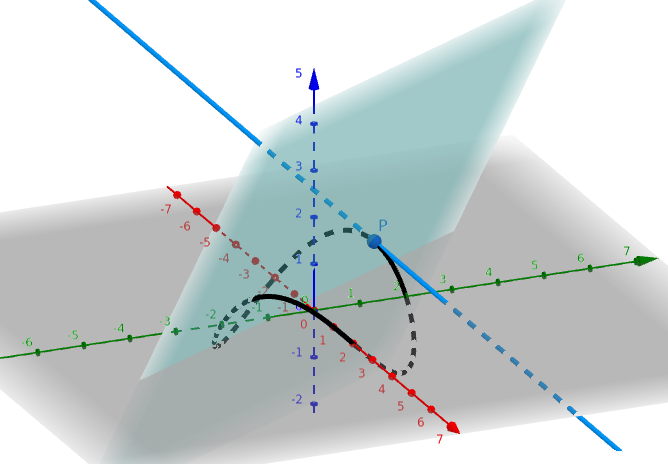
\includegraphics[scale=0.4]{tangent_line.png}
\end{figure}
\end{example}

\subsubsection{Приблизне обчислення}
$z-f(\vec{x}) = o(||\vec{x}-\vec{x}^0||)$\\
Якщо $\vec{x}_0$ близлький до $\vec{x}$, тобто $||\vec{x} - \vec{x}^0|| << 1$, то тоді\\
$f(\vec{x})-z \approx 0$\\
$\Rightarrow f(\vec{x}) \approx z^0 + \departial{f}{x_1}(\vec{x}^0)(x_1-x_1^0) + \dots + \departial{f}{x_n}(\vec{x}^0)(x_n-x_n^0)$
\bigline


\subsection{Диференціювання та похідні старших порядків}
\begin{definition}
Задано функцію $f: A \to \mathbb{R}$ та $\vec{x}^0 \in A$ - внутрішня точка. Також $f$ - диференційована в т. $\vec{x}^0$.\\
\textbf{Частковими похідними другого роду} від функції $f$ в т. $\vec{x}^0$ називається вираз:
\begin{align*}
\dfrac{\partial}{\partial x_j} \left( \dfrac{\partial f}{\partial x_k} (\vec{x}^0) \right) = \dfrac{\partial^2 f}{\partial x_j \partial x_k} (\vec{x}^0)
\end{align*}
\end{definition}

\begin{example}
Знайдемо всі часткові похідні другого порядку функції $f(x,y) = x^4+y^4-4x^2y^2$.\\
$\departial{f}{x} = 4x^3 - 8xy^2 \implies \begin{cases} \seconddepartial{f}{x}{x} = 12x^2 - 8y^2 \\ \seconddepartial{f}{y}{x} = -16xy \end{cases}$ \hspace{1cm} $\departial{f}{y} = 4y^3 - 8x^2y \implies \begin{cases} \seconddepartial{f}{x}{y} = -16xy \\ \seconddepartial{f}{y}{y} = 12y^2-8x^2 \end{cases}$.\\
Можемо зауважити, що $\seconddepartial{f}{y}{x} = \seconddepartial{f}{x}{y}$. Проте в загальному випадку це не так.
\end{example}

\begin{example}
Розглянемо функцію $f(x,y) = \begin{cases} xy \dfrac{x^2-y^2}{x^2+y^2} & (x,y) \neq (0,0) \\ 0 & (x,y) = (0,0) \end{cases}$. Зосередимось лише на знаходженні $\seconddepartial{f}{y}{x}(0,0), \seconddepartial{f}{x}{y}(0,0)$.\\
$\departial{f}{x} = \begin{cases} y\dfrac{x^4-y^4+4x^2y^2}{(x^2+y^2)^2} & (x,y) \neq (0,0) \\ 0 & (x,y) = (0,0) \end{cases}$ \hspace{1cm} $\departial{f}{y} = \begin{cases} -x\dfrac{y^4-x^4+4x^2y^2}{(x^2+y^2)^2} & (x,y) \neq (0,0) \\ 0 & (x,y) = (0,0) \end{cases}$\\
$\seconddepartial{f}{x}{y}(0,0) = \huge\lim_{\Delta x \to 0} \dfrac{\departial{f}{y}(\Delta x, 0) - \departial{f}{y}(0,0)}{\Delta x} = 1$ \hspace{1cm} $\seconddepartial{f}{y}{x}(0,0) = \huge\lim_{\Delta y \to 0} \dfrac{\departial{f}{x}(0, \Delta y) - \departial{f}{x}(0,0)}{\Delta y} = -1$\\
Таким чином, $\seconddepartial{f}{y}{x} \neq \seconddepartial{f}{x}{y}$.
\end{example}

\begin{theorem}
Задано функцію $f: A \to \mathbb{R}$ та $\vec{x}^0 \in A$ - внутрішня точка. Відомо, що $\exists \dfrac{\partial^2 f}{\partial x_j \partial x_k} (\vec{x}), \dfrac{\partial^2 f}{\partial x_k \partial x_j} (\vec{x})$ в околі т. $\vec{x}^0$ та є неперервними в т. $\vec{x}^0$.\\
Тоді $\seconddepartial{f}{x_j}{x_k} = \seconddepartial{f}{x_k}{x_j}$.
\end{theorem}

\begin{proof}
\textit{Ми будемо доводити, коли $m = 2$. Для більших аргументів - аналогічно, але більш технічна справа}
\bigskip \\
Отже, дано $f(x,y)$ та в околі т. $(x_0,y_0)$ існують часткові похідні другого порядку $\exists \dfrac{\partial^2 f}{\partial x \partial y}, \dfrac{\partial^2 f}{\partial y \partial x}$ які неперервні в $(x_0,y_0)$.\\
Розглянемо вираз $\Delta = f(x_0+\Delta x, y_0+\Delta y) - f(x_0+\Delta x,y_0) - f(x_0,y_0+\Delta y) + f(x_0,y_0)$.\\
Покладемо функцію $k(s) = f(s,y_0+\Delta y) - f(s,y_0), s \in [x_0,x_0+\Delta x]$. Тоді $\Delta = k(x_0+\Delta x) - k(x_0)$.\\
$k'(s) = (f(s,y_0+\Delta y) - f(s,y_0))'_s = \departial{f}{s}(s,y_0+\Delta y) - \departial{f}{s}(s,y_0)$.\\
Оскільки нам відомі другі часткові похідні, то зрозуміло, що в нас існує $\departial{f}{x}, \departial{f}{y}$, причому в тому самому околі т. $(x_0,y_0)$. Тобто звідси $k$ - диференційована на $[x_0, x_0+\Delta x]$, тоді за теоремою Лагранжа, $\exists \xi_1 \in (x_0,x_0+\Delta x): \Delta = k(x_0+\Delta x) - k(x_0) = k'(\xi_1) \Delta x = \left( \departial{f}{s}(\xi_1,y_0+\Delta y) - \departial{f}{s}(\xi_1,y_0) \right) \Delta x$.\\
Покладемо функцію $m(t) = \departial{f}{s}(\xi_1,t), t \in [y_0,y_0+\Delta y]$. Тоді $\Delta = (m(y_0+\Delta y) - m(y_0)) \Delta x$.\\
$m'(t) = \left( \departial{f}{s}(\xi_1,t) \right)'_t = \departial{}{t}\left( \departial{f}{s}(\xi_1,t) \right) = \seconddepartial{f}{t}{s}(\xi_1,t)$.\\
Похідна дійсно існує за умовою теореми, тобто $m$ - диференційована на $[y_0,y_0+\Delta y]$, тоді за теоремою Лагранжа, $\exists \eta_1 \in (y_0,y_0+\Delta y): \Delta = (m(y_0+\Delta y)-m(y_0)) \Delta x = m'(\eta_1) \Delta y \Delta x = \seconddepartial{f}{t}{s}(\xi_1,\eta_1) \Delta y \Delta x$.
\bigskip \\
Повернімось до виразу $\Delta = f(x_0+\Delta x, y_0+\Delta y) - f(x_0+\Delta x,y_0) - f(x_0,y_0+\Delta y) + f(x_0,y_0)$, ми розглянемо її з іншої сторони.\\
Покладемо функцію $p(t) = f(x_0+\Delta x,t) - f(x_0,t), t \in [y_0,y_0+\Delta y]$. Тоді $\Delta = p(y_0+\Delta y) - p(y_0)$.\\
А далі я буду просто продовжувати рівність, міркування аналогічні, що пов'язані зі застосуванням теореми Лагранжа двічі:\\
$\Delta = p(y_0+\Delta y) - p(y_0) = p'(\eta_2) \Delta y = (f(x_0+\Delta x, t) - f(x_0,t))'_t (\eta_2) \Delta y = \left( \departial{f}{t}(x_0+\Delta x, \eta_2) - \departial{f}{t}(x_0,\eta_2) \right) \Delta y \boxed{=}$\\
$q(s) = \departial{f}{t}(s, \eta_2)$\\
$\boxed{=} (q(x_0+\Delta x) - q(x_0))\Delta y = q'(\xi_2) \Delta x \Delta y = \left( \departial{f}{t}(s,\eta_2) \right)'_s (\xi_2) \Delta x \Delta y = \seconddepartial{f}{s}{t}(\xi_2,\eta_2) \Delta x \Delta y$.\\
Зауважу, що $\eta_2 \in (y_0,y_0+\Delta y), \xi_2 \in (x_0,x_0+\Delta x)$.
\bigskip \\
Отримали таку рівність: $\seconddepartial{f}{t}{s}(\xi_1,\eta_1) \Delta y \Delta x = \seconddepartial{f}{s}{t}(\xi_2,\eta_2) \Delta x \Delta y \implies \seconddepartial{f}{t}{s}(\xi_1,\eta_1) = \seconddepartial{f}{s}{t}(\xi_2,\eta_2)$.\\
Нарешті, за умовою задачі, другі часткові похідні є неперервними в т. $(x_0,y_0)$, тому далі одночасно прямуємо $x \to x_0, y \to y_0 \implies \Delta x \to 0, \Delta y \to 0$. Оскільки $\xi_1,\xi_2 \in (x_0,x_0+\Delta x) \hspace{0.2cm} \eta_1,\eta_2 \in (y_0,y_0+\Delta y)$, то звідси $\xi_1,\xi_2 \to x_0$ та $\eta_1,\eta_2 \to y_0$.\\
Остаточно отримаємо $\seconddepartial{f}{y}{x}(x_0,y_0) = \seconddepartial{f}{x}{y}(x_0,y_0)$ (літери $s,t$ я замінив на $x,y$, результат не зміниться).
\end{proof}

\begin{definition}
Задано функцію $f: A \to \mathbb{R}$ та $\vec{x}^0 \in A$ - внутрішня точка.\\
Функція $f$ називається \textbf{двічі диференційованою в т.} $\vec{x}^0$, якщо всі часткові похідні існують в околі т. $\vec{x}^0$ та диференційовані в т. $\vec{x}^0$.
\end{definition}

\begin{example}
Маємо функцію $z = x^2+2y^2-5xy$. З'ясуємо, чи буде ця функція двічі диференційованою.\\
$\departial{z}{x} = 2x-5y$ \hspace{1cm} $\departial{z}{y} = 4y-5x$\\
Усі отримані часткові похідні існують в будь-якому околі деякої точки.\\
$\seconddepartial{z}{x}{x} = 2$ \hspace{1cm} $\seconddepartial{z}{y}{x} = -5$\\
Отримані часткові похідні визначені та неперервні в будь-якій точці. Таким чином, за \textbf{Th.4.1.8.}, функція $\departial{z}{x}$ - диференційована.
$\seconddepartial{z}{x}{y} = -5$ \hspace{1cm} $\seconddepartial{z}{y}{y} = 4$\\
Отримані часткові похідні визначені та неперервні в будь-якій точці. Таким чином, за \textbf{Th.4.1.8.}, функція $\departial{z}{y}$ - диференційована.\\
Отже, за означенням, $z$ - двічі диференційована функція.
\end{example}

\begin{proposition}
Функція $f$ двічі диференційована в т. $\vec{x}^0$ $\iff$ $\textrm{grad} f$ - диференційована в т. $\vec{x}^0$.
\iffalse
\begin{align*}
\textrm{grad} f(\vec{x}) - \textrm{grad} f(\vec{x}^0) = M \Delta \vec{x} + o(\Norm{\Delta \vec{x}}), \Delta \vec{x} \to \vec{0}
\end{align*}
де $M$ - матриця всіх часткових похідних $\textrm{grad} f(\vec{x})$ - \textbf{матриця Гесе}
\begin{align*}
f''(\vec{x}) = M = \begin{pmatrix}
\dfrac{\partial^2 f}{(\partial x_1)^2} & \dfrac{\partial^2 f}{\partial x_2 \partial x_1} & \dots & \dfrac{\partial^2 f}{\partial x_n \partial x_1} \\
\dfrac{\partial^2 f}{\partial x_1 \partial x_2} & \dfrac{\partial^2 f}{(\partial x_2)^2} & \dots & \dfrac{\partial^2 f}{\partial x_n \partial x_2} \\
\vdots & \vdots & \ddots & \vdots \\
\dfrac{\partial^2 f}{(\partial x_1 \partial x_n} & \dfrac{\partial^2 f}{\partial x_2 \partial x_n} & \dots & \dfrac{\partial^2 f}{(\partial x_n)^2} \\
\end{pmatrix}(\vec{x})
\end{align*}
\fi
\end{proposition}

\begin{proof}
Дійсно, $f$ - двічі диференційована в т. $\vec{x}^0 \iff \forall j=\overline{1,m}: \exists \departial{f}{x_j}$ - диференційована в т. $\vec{x}^0 \iff \text{grad} f = \begin{pmatrix}
\departial{f}{x_1} \\ \vdots \\ \departial{f}{x_m}
\end{pmatrix}$ - як вектор-функція - диференційована в т. $\vec{x}^0$.
\end{proof}

Розпишемо диференційованість вектор-функції $\wordgrad f$ в т. $\vec{x}^0$ за означенням:\\
$\wordgrad f(\vec{x}^0+\Delta \vec{x}) - \wordgrad f(\vec{x}^0) = M \Delta \vec{x} + \vec{o}(\Norm{\Delta \vec{x}}), \Delta \vec{x} \to \vec{0}$.\\
Звідси ми маємо, що $M = \begin{pmatrix}
\departial{}{x_1} \left( \departial{f}{x_1} \right) & \dots & \departial{}{x_m} \left( \departial{f}{x_1} \right) \\
\vdots & \ddots & \vdots \\
\departial{}{x_1} \left( \departial{f}{x_m} \right) & \dots & \departial{}{x_m} \left( \departial{f}{x_m} \right)
\end{pmatrix} = \\ = \begin{pmatrix}
\seconddepartial{f}{x_1}{x_1} & \dots & \seconddepartial{f}{x_m}{x_1} \\
\vdots & \ddots & \vdots \\
\seconddepartial{f}{x_1}{x_m} & \dots & \seconddepartial{f}{x_m}{x_m}
\end{pmatrix} (\vec{x}^0) = H(\vec{x}^0) = f''(\vec{x}^0)$ - \textbf{матриця Гесе}\\
Матриця Гесе описує \textbf{другу похідну} функції $f$ в т. $\vec{x}^0$ та одночасно \textbf{похідну} вектор-функції $\wordgrad f$ в т. $\vec{x}^0$. Якщо матриця буде квадратною, то ми можемо обчислити $\det f''(\vec{x}^0)$ - \textbf{гесіан}.

\begin{definition}
Задано функцію $f: A \to \mathbb{R}$ та $\vec{x}^0 \in A$ - внутрішня точка. Також $f$ - диференційована в т. $\vec{x}^0$.\\
\textbf{Другим диференціалом} функції $f$ називають вираз:
\begin{align*}
d^2f(\vec{x}^0) = d(df(\vec{x}^0))
\end{align*}
\end{definition}
З'ясуємо, як цей вираз можна по-інакшому записати. Маємо:\\
$d^2 f = d\left( df \right) = d\left( \departial{f}{x_1}\,dx_1 + \dots + \departial{f}{x_m}\,dx_m \right) = d \left(\departial{f}{x_1}\,dx_1\right) + \dots + d\left( \departial{f}{x_m}\,dx_m \right) = \\ = d \left(\departial{f}{x_1}\right)\,dx_1 + \dots + d\left( \departial{f}{x_m}\right)\,dx_m = \left( \departial{}{x_1} \left( \departial{f}{x_1} \right)\,dx_1 + \dots + \departial{}{x_m} \left( \departial{f}{x_1} \right)\,dx_m \right)\,dx_1 + \dots + \left( \departial{}{x_1} \left( \departial{f}{x_m} \right)\,dx_1 + \dots + \departial{}{x_m} \left( \departial{f}{x_m} \right)\,dx_m \right)\,dx_m = \\ = \left(\seconddepartial{f}{x_1}{x_1}\,dx_1^2 + \dots + \seconddepartial{f}{x_m}{x_1}\,dx_m \,dx_1 \right) + \dots  + \left(\seconddepartial{f}{x_1}{x_m}\,dx_1 \,dx_m + \dots + \seconddepartial{f}{x_m}{x_m}\,dx_m^2 \right) = \huge\sum_{i,j=1}^m \seconddepartial{f}{x_i}{x_j}\,dx_i\,dx_j$.\\
Отже, маємо іншу формулу для другого диференціалу в т. $\vec{x}^0$:
\begin{align*}
d^2 f(\vec{x}^0) = \huge\sum_{i,j=1}^m \seconddepartial{f}{x_i}{x_j} (\vec{x}^0)\,dx_i\,dx_j
\end{align*}
Або це можна записати в \textquotedbl лінійно-алгебраїчному\textquotedbl{} вигляді:
\begin{align*}
d^2 f(\vec{x}^0) = \left( \departial{}{x_1}\,dx_1 + \dots + \departial{}{x_m}\,dx_m \right)^2 f(\vec{x}^0)
\end{align*}

\begin{example}
Знайдемо другий диференціал функції $z = x^3 + 2y^2 - 5xy$.\\
Ми вже шукали другі часткові похідні $\seconddepartial{f}{x}{x} = 6x \hspace{0.5cm} \seconddepartial{f}{x}{y} = \seconddepartial{f}{y}{x} = -5 \hspace{0.5cm} \seconddepartial{f}{y}{y} = 4$. Таким чином,\\
$d^2z = \seconddepartial{f}{x}{x}\,dx^2 + 2\seconddepartial{f}{x}{y}\,dx\,dy + \seconddepartial{f}{y}{y}\,dy^2 = 6x\,dx^2 -10\,dx\,dy +4\,dy^2$.
\end{example}

\begin{definition}
Задано функцію $f: A \to \mathbb{R}$ та $\vec{x}^0 \in A$ - внутрішня точка. Також $f$ - $m$ разів диференційована в т. $\vec{x}^0$.\\
\textbf{Частковим похідним} $m+1$-го порядку в т. $\vec{x}^0$ називають похідну:
\begin{align*}
\dfrac{\partial}{\partial x_{j_{m+1}}} \left( \dfrac{\partial^m f}{\partial x_{j_1} \partial x_{j_2} \dots \partial x_{j_m}} \right)(\vec{x}^0) = \dfrac{\partial^{m+1} f}{\partial x_{j_{m+1}} \partial x_{j_1} \partial x_{j_2} \dots \partial x_{j_m}}(\vec{x}^0) \\
j_1+j_2+\dots+j_m+j_{m+1} = m+1
\end{align*}
\end{definition}

\begin{remark}
Що таке \textbf{похідна} $m$-го порядку, визначати не буду, бо ще рано.
\end{remark}

\subsection{Формула Тейлора}
Зробимо певні позначення:
\begin{align*}
[\vec{x}^0, \vec{x}] = \{(1-t)\vec{x}^0 + t \vec{x} : t \in [0,1]\} \\
(\vec{x}^0, \vec{x}) = \{(1-t)\vec{x}^0 + t \vec{x} : t \in (0,1)\}
\end{align*}

\begin{theorem}[Теорема Тейлора (у формі Лагранжа)]
Задано функцію $f: A \to \mathbb{R}$ та $\vec{x}^0 \in A$ - внутрішня точка. Відомо, що $f$ - диференційована $n+1$ разів в околі т. $\vec{x}^0$. Тоді $\exists \vec{\xi} \in (\vec{x}^0,\vec{x})$ або $(\vec{x},\vec{x}^0)$, для якого\\
$f(\vec{x}) = f(\vec{x}^0) + \dfrac{f'(\vec{x}^0)}{1!}(\vec{x}-\vec{x}^0) + \dfrac{f''(\vec{x}^0)}{2!}(\vec{x}-\vec{x}^0)^2 + \dots  + \dfrac{f^{(n)}(\vec{x}^0)}{m!}(\vec{x}-\vec{x}^0)^{n} + \dfrac{f^{(n+1)}(\vec{\xi})}{(n+1)!}(\vec{x}-\vec{x}^0)^{n+1}$\\
Під виразами $f^{(k)}(\vec{x}-\vec{x}^0)^k$ я розумію як диференціал $d^{k} f(\vec{x}^0)$, що має свою формулу: \\ $d^{k} f(\vec{x}^0) = \huge\sum_{j_1,\dots,j_k = 1}^m \dfrac{\partial^k f}{\partial x_{j_1}\dots \partial x_{j_k}}(\vec{x}^0) \cdot \,dx_{j_1} \dots \,dx_{j_k}$\\
Замість $dx_{j_1} \dots \,dx_{j_k}$ можна писати $(x_{j_1}-x_{j_1}^0) \dots (x_{j_k}-x_{j_k}^0)$.
\end{theorem}

\begin{proof}
Розглянемо функцію $p(t) = f(\vec{x}^0 + t(\vec{x} - \vec{x}^0))$, тут $|t| \leq 1$ - функція від однієї змінної.\\
Знайдемо похідні від цієї функції:\\
$p'(t) = f(\vec{x}^0 + t(\vec{x}-\vec{x}^0))'_t = (f(x_1+t(x_1-x_1^0),\dots,x_m+t(x_m-x_m^0)))'_t = (f(u_1,\dots,u_m))'_t = \\ = \departial{f}{u_1} \departial{u_1}{t} + \dots + \departial{f}{u_m} \departial{u_m}{t} = \departial{f}{u_1} (x_1-x_1^0) + \dots + \departial{f}{u_m} (x_m-x_m^0) = \begin{pmatrix}
\departial{f}{u_1} & \dots & \departial{f}{u_m}
\end{pmatrix} \begin{pmatrix}
x_1-x_1^0 \\ \vdots \\ x_m-x_m^0
\end{pmatrix} = \\ = f'(\vec{x}^0+t(\vec{x}-\vec{x}^0)) (\vec{x}-\vec{x}^0)$\\
$p''(t) = [f'(\vec{x}^0 + t(\vec{x}-\vec{x}^0)) \cdot (\vec{x}-\vec{x}^0)]'_t \overset{\text{аналогічно}}{=} f''(\vec{x}^0+t(\vec{x}-\vec{x}^0))(\vec{x}-\vec{x}^0)^2$\\
$\vdots$ \\
$p^{(k)}(t) = f^{(k)}(\vec{x}^0 + t(\vec{x}-\vec{x}^0))^k$.\\
Коротше, наша функція $n+1$ разів диференційована на $[0,1]$. Тому ми можемо розкласти формулу Тейлора як функцію з однією змінною. $\exists \xi \in (0,1):$\\
$p(t) = p(0) + \dfrac{p'(0)}{1!}(1-0) + \dfrac{p''(0)}{2!}(1-0)^2 + \dots + \dfrac{p^{(n)}(0)}{n!}(1-0)^{n} + \dfrac{p^{(n+1)}(\xi)}{(n+1)!}(1-0)^{n+1}$.\\
А далі підставляємо все, що маємо:\\
$p(0) = f(\vec{x}^0)$\\
$p'(0) = f'(\vec{x}^0)(\vec{x}-\vec{x}^0)$\\
$p''(0) = f''(\vec{x}^0)(\vec{x}-\vec{x}^0)^2$\\
$\vdots$\\
$p^{(n+1)}(\xi) = f^{(n+1)}(\vec{x}^0+\xi (\vec{x}-\vec{x}^0)(\vec{x}-\vec{x}^0)^{n+1}$\\
Отже, $f(\vec{x}) = f(\vec{x}^0) + \dfrac{f'(\vec{x}^0)}{1!}(\vec{x}-\vec{x}^0) + \dfrac{f''(\vec{x}^0)}{2!}(\vec{x}-\vec{x}^0)^2 + \dots  + \dfrac{f^{(n)}(\vec{x}^0)}{n!}(\vec{x}-\vec{x}^0)^n + \dfrac{f^{(n+1)}(\vec{\xi})}{(n+1)!}(\vec{x}-\vec{x}^0)^{n+1}$,\\
де $\vec{\xi} = \vec{x}^0 + \xi (\vec{x}-\vec{x}^0) \in (\vec{x}^0,\vec{x})$.
\end{proof}

Можна обережно довести, що $\dfrac{f^{(n+1)}(\vec{\xi})}{(n+1)!}(\vec{x}-\vec{x}^0)^{n+1} = o(\Norm{\vec{x}-\vec{x}^0}^{n}), \vec{x} \to \vec{x}^0$. Тоді матимемо формулу Тейлора в формі Пеано:\\
$f(\vec{x}) = f(\vec{x}^0) + \dfrac{f'(\vec{x}^0)}{1!}(\vec{x}-\vec{x}^0) + \dfrac{f''(\vec{x}^0)}{2!}(\vec{x}-\vec{x}^0)^2 + \dots + \dfrac{f^{(n)}(\vec{x}^0)}{n!}(\vec{x}-\vec{x}^0)^{n} + o(\Norm{\vec{x}-\vec{x}^0}^{n}), \vec{x} \to \vec{x}^0$.

\begin{example}
Розкласти функцію $f(x,y) = e^{x+y}$ відносно т. $(x_0,y_0) = (1,-1)$.\\
Заздалегідь зауважимо, що $\dfrac{\partial^s f}{\partial x^{s_1} \partial y^{s_2}}(1,-1) = e^{x+y} |_{(1,-1)} = 1$, де $s_1 + s_2 = s$.\\
$f(1,-1) = 1$\\
$f'(1,-1)(\vec{x}-\vec{x}^0) = (x-1) + (y+1)$\\
$f''(1,-1)(\vec{x}-\vec{x}^0)^2 = (x-1)^2 + 2(x-1)(y+1) + (y+1)^2$\\
$f'''(1,-1)(\vec{x}-\vec{x}^0)^3 = (x-1)^3 + 3(x-1)^2(y+1) + 3(x-1)(y+1)^2 + (y+1)^3$\\
$\vdots$\\
Таким чином, ми можемо це записати ось так:\\
$f(x,y) = 1 + \left[\dfrac{(x-1)}{1!} + \dfrac{(y+1)}{1!} \right] + \left[ \dfrac{(x-1)^2}{2!} + \dfrac{2(x-1)(y+1)}{2!} + \dfrac{(y+1)^2}{2!} \right] + \dots + \\ + \left[\dfrac{(x-1)^n}{n!} + \dfrac{C_2^n(x-1)^{n-1}(y+1)}{n!} + \dots + \dfrac{(y+1)^n}{n!} \right] + o\left(\sqrt{(x-1)^2+(y+1)^2}\right) = \\
= \huge\sum_{k=1}^n \sum_{p=0}^k \dfrac{C_k^p}{k!}(x-1)^{k-p} (y+1)^p + o\left(\sqrt{(x-1)^2+(y+1)^2}\right), (x,y) \to (1,-1)$.
\end{example}

\begin{remark}
Можна формулу Тейлора записати в якості ряда Тейлора за певними умовами, але я цього робити не буду.
\end{remark}

\subsection{Локальні екстремуми}
\begin{definition}
Задано функцію $f:A\to \mathbb{R}$ та $\vec{x}^0 \in A$ - внутрішня точка.\\
Точка $\vec{x}^0$ називається точкою:\\
- \textbf{локального максимуму}, якщо $\exists U_{\varepsilon}(\vec{x}^0): \forall \vec{x} \in U_{\varepsilon}(\vec{x}^0): f(\vec{x}^0) \geq f(\vec{x})$;\\
- \textbf{локального мінімуму}, якщо $\exists U_{\varepsilon}(\vec{x}^0): \forall \vec{x} \in U_{\varepsilon}(\vec{x}^0): f(\vec{x}^0) \leq f(\vec{x})$.\\
для строгих екстремумів нерівність строга та існують околи $U_\varepsilon(\vec{x}^0) \setminus \{\vec{x}^0\}$.
\end{definition}

\begin{theorem}[Необхідна умова локального екстремуму]
Задано функцію $f: A \to \mathbb{R}$ така, що має всі часткові похідні в т. $\vec{x}^0 \in A$ - внутрішня.\\
Відомо, що $\vec{x}^0$ - локальний екстремум. Тоді $\departial{f}{x_j}(\vec{x}^0) = 0, \forall j=\overline{1,m}$.
\end{theorem}

\begin{proof}
Розглянемо функцію $h(x_1) = f(x_1,x_2^0,\dots,x_m^0)$ - функція від однієї змінної, така, що $x_1^0$ - локальний екстремум. Для інших змінних аналогічно. Більш того, $h'(x_1) = \departial{f}{x_1}(x_1,x_2^0,\dots,x_m^0)$.\\
Таким чином, за необхідною умовою локального екстремуму матана 1 семестру, \\ $h'(x_1) = 0 \implies \departial{f}{x_1}(x_1^0,x_2^0,\dots,x_m^0) = 0$.
\end{proof}

\begin{definition}
Точка $\vec{x}^0$ називається \textbf{критичною} для функції $f$, якщо всі часткові похідні в заданній точці нулеві.
\end{definition}

\textit{Надалі вважається, що ви ознайомлені з означенням додатньо/від'ємно визначеними матрицями та з критерієм Сільвестра.}

\begin{lemma}
Задано симетричну матрицю $B(\vec{x}) = \begin{pmatrix}
b_{11}(\vec{x}) & \dots & b_{1m}(\vec{x}) \\
\vdots & \ddots & \vdots \\
b_{1m}(\vec{x}) & \dots & b_{mm}(\vec{x}) \\
\end{pmatrix}$ - неперервна на множині $A$ та т. $\vec{x}^0 \in A$ - внутрішня точка. Відомо, що $B(\vec{x}^0)$ - строго додатньо/від'ємно визначена. \\ Тоді в деякому околі т. $\vec{x}^0$ матриця $B(\vec{x})$ - строго додатня/від'ємно визначена.
\end{lemma}

\begin{proof}
Будемо доводити для випадку строго додатньої визначеності.\\
За умовою, $B(\vec{x}) \in C(A)$, тобто всі функції в матриці неперервні. Обчислюючи кутові мінори $\Delta_k, k = \overline{1,n}$, отримаємо, що $\Delta_k \in C(A)$ за властивостями неперервності.\\
За критерієм Сільвества, маємо $\forall k = \overline{1,m}: \Delta_k (\vec{x}^0) > 0$. Оскільки $\vec{x}^0$ - внутрішня та $\Delta_k \in C(A)$, то $\exists U_{\delta_k}(\vec{x}^0)$, де $\forall \vec{x} \in U_{\delta_k}(\vec{x}^0): \Delta_k(\vec{x}) > 0$.\\
Оберемо $\varepsilon = \min \{\delta_1, \dots, \delta_m \}$, тоді $\forall \vec{x} \in U_{\delta}(\vec{x}^0): \forall k = \overline{1,n}: \Delta_k(\vec{x}) > 0$.\\
Тоді за критерієм Сильвестра, $B(\vec{x})$ - строго додатньо визначена в околі $U_\delta (\vec{x}^0)$.
\end{proof}

\begin{corollary}
Якщо матриця $B(\vec{x}^0)$ - знако невизначена, то в деякому околі т. $\vec{x}^0$ матриця $B(\vec{x})$ - знако не визначена.
\end{corollary}

\begin{proof}
!Припустимо, що в будь-якому околі $U_\delta (\vec{x}^0)$ знайдеться $\vec{x}_\delta$, для якої $B(\vec{x}_\delta)$ - строго додатно визначена.\\
Покладемо $\delta = \dfrac{1}{n}$, тоді $\exists \vec{x}^{(n)}: \Norm{\vec{x}^0 - \vec{x}^{(n)}} < \dfrac{1}{n}$, але $B(\vec{x}^{(n)})$ - строго додатно визначена.\\
Якщо $\vec{x}^{(n)} \to \vec{x}^{0}$, то за неперервністю, $B(\vec{x}^{(n)}) \to B(\vec{x}^0)$, звідси оскільки $(B(\vec{x}^{(n)}) \vec{t}, \vec{t}) > 0, \forall \vec{t}$, то тоді $(B(\vec{x}^{0}) \vec{t}, \vec{t}) \geq 0, \forall \vec{t}$. Тобто матриця $\vec{B}(\vec{x}^0)$ - невід'ємно визначена. Суперечність!\\
Якщо припускати строго від'ємну визначеність, то міркування аналогічні.
\end{proof}


\begin{theorem}[Достатня умова локального екстремуму]
Задано функцію $f: A \to \mathbb{R}$, таку, що $f$ - двічі неперервно-диференційована в околі т. $\vec{x}^0 \in A$ - критична точка.\\
1) Нехай $f''(\vec{x}^0)$ - строго додатньо визначена. Тоді $\vec{x}^0$ - строгий локальний мінімум;\\
2) Нехай $f''(\vec{x}^0)$ - строго від'ємно визначена. Тоді $\vec{x}^0$ - строгий локальний максимум;\\
3) Нехай $f''(\vec{x}^0)$ - знако-невизначена. Тоді $\vec{x}^0$ - не локальний екстремум.
\end{theorem}

\begin{proof}
1) $f''(\vec{x}^0)$ - строго додатньо визначена. Тоді за лемою, $\exists U_{\delta}(\vec{x}^0): \forall \vec{x} \in U_{\delta}(\vec{x}^0): f''(\vec{x})$ - строго додатньо визначена. Ми т. $\vec{x}$ зафіксуємо.\\
За умовою, $\vec{x}^0$ - критична точка $\implies f'(\vec{x}^0) = \vec{0}$. Запишемо функцію у вигляді формули Тейлора до другої похідної:\\
$f(\vec{x}) = f(\vec{x}^0) + \dfrac{f'(\vec{x}^0)}{1!}(\vec{x}-\vec{x}^0) + \dfrac{f''(\vec{\xi})}{2!}(\vec{x}-\vec{x}^0)^2$, де $\vec{\xi} \in (\vec{x}^0,\vec{x})$ або $(\vec{x},\vec{x}^0)$.\\
$\implies f(\vec{x}) - f(\vec{x}^0) = \dfrac{1}{2} \left(f''(\vec{\xi})(\vec{x}-\vec{x}^0), (\vec{x}-\vec{x}^0) \right)$. Зокрема $f''(\vec{\xi})$ - також додатньо визначена, а тому за означенням, $\left( f''(\vec{\xi})(\vec{x}-\vec{x}^0),(\vec{x}-\vec{x}^0) \right) > 0$. Звідси $f(\vec{x})-f(\vec{x}^0) > 0 \\ \implies \forall \vec{x} \in U_{\varepsilon}(\vec{x}^0): f(\vec{x}) > f(\vec{x}^0) \implies \vec{x}^0$ - локальний мінімум.
\bigskip \\

2) Аналогічно до 1).
\bigskip \\

3) Дороговцев пише ось що:\\
зауважимо, що якщо $f''(\vec{x}^0)$ знако невизначена, то для будь-якого окілу $U_\delta (\vec{0})$ будуть існувати вектори $\vec{a}, \vec{b}$, щоб $f''(\vec{x}^0) \vec{a}^2 > 0$ та $f''(\vec{x}^0) \vec{b} < 0$. (це єдине, шо я не розумію).
\iffalse
$f''(\vec{x}^0)$ - знако-невизначена. Тоді за наслідком леми, $\exists U_\delta (\vec{x}^0): \forall \vec{x} \in U_\delta (\vec{x}^0): f''(\vec{x})$ - знако-невизначена.\\
Маємо $f(\vec{x}) - f(\vec{x}^0) = \dfrac{1}{2} \left(f''(\vec{\xi})(\vec{x}-\vec{x}^0), (\vec{x}-\vec{x}^0) \right)$, $\vec{\xi} \in (\vec{x}^0,\vec{x})$ або $(\vec{x},\vec{x}^0)$. \\ Зокрема в т. $\vec{\xi}$ матриця $f''(\vec{\xi})$ - знако-невизначена. За означенням
Тоді за попередними пунктами, $f(\vec{x}^0) < f(\vec{x}_1)$ та $f(\vec{x}^0) > f(\vec{x}_2)$, що порушують означення локального екстремуму для т. $\vec{x}^0$
\fi
\end{proof}

\subsection{Умовні локальні екстремуми}
\begin{definition}
Задано функцію $f: A \to \mathbb{R}$ та $A$ - відкрита множина. Задано систему функцій $\phi_j: A \to \mathbb{R}$, де $j = \overline{1,s}, s < m$. Покладемо множину $M = \{\vec{x} \in A: \phi_j(\vec{x}) = 0, j = \overline{1,s} \}$.\\
\iffalse
$\rank \begin{pmatrix}
\departial{\phi_1}{x_1} & \dots & \departial{\phi_1}{x_n} \\
\vdots & \ddots & \vdots \\
\departial{\phi_s}{x_1} & \dots & \departial{\phi_s}{x_n}
\end{pmatrix}(\vec{x}^0) = s$ - деякий максимально можливий ранг.\\
\fi
Тоді рівняння $\phi_j(\vec{x}) = 0, j=\overline{1,s}$ називають \textbf{рівняннями зв'язку}.\\
Точка $\vec{x}^0 \in M$ називається \textbf{умовним локальним}:\\
- \textbf{максимумом}, якщо $\exists U_{\varepsilon}(\vec{x}^0): \forall \vec{x} \in M \cap U_{\varepsilon}(\vec{x}^0): f(\vec{x}^0) \geq f(\vec{x})$ \\
- \textbf{мінімумом}, якщо $\exists U_{\varepsilon}(\vec{x}^0): \forall \vec{x} \in M \cap U_{\varepsilon}(\vec{x}^0): f(\vec{x}^0) \leq f(\vec{x})$\\
Для строгих екстремумів нерівність строга та існують околи $U_\varepsilon (\vec{x}^0) \setminus \{\vec{x}^0\}$.
\end{definition}

\begin{example}
Маємо функцію $z = x^2+y^2$ та рівняння зв'язку $\phi_1(x,y) = x^2+y^2-25=0$. Вона має умовні екстремуми в т. $(3,4), (-3,-4)$ на множині $M$. Як їх шукати, дізнаємось потім.
\end{example}

Одразу формулювати теорему буде складно, тому ми будемо спочатку будувати наші роздуми, як зрозуміти, що $\vec{x}^0$ - умовний локальний екстремум
\bigline
Маємо множину $M=\{\vec{x}: \phi_j(\vec{x}) = 0, j=\overline{1,s} \}$ та $\vec{x}^0$ - локальний екстремум\\
Розглянемо диференційовану криву $\gamma = \{\vec{x}(t), t \in (-\delta, \delta )\} \subset M \cap U_{\varepsilon}(\vec{x}^0)$, причому нехай $\vec{x}(0) = \vec{x}^0$\\
Функцію $f(\vec{x})$ звузимо на криву $\gamma$ - отримаємо функцію $h(t) = f(\vec{x}(t))$, де має локальний екстремум в т. $t_0 = 0$. Тоді за необхідною умовою, $h'(0) = 0$\\
З іншого боку, $h'(0) = f'(\vec{x}(0)) \cdot \vec{x}'(0) \boxed{=}$\\
Тут $f'(\vec{x}(0)) = \begin{pmatrix}
\departial{f}{x_1}(\vec{x}(0)) & \dots & \departial{f}{x_n}(\vec{x}(0))
\end{pmatrix}$\\
А також $\vec{x}'(0) = \begin{pmatrix}
x_1'(0) & \dots & x_n'(0)
\end{pmatrix}$\\
Множимо два вектори скалярно\\
$\boxed{=} \departial{f}{x_1}(\vec{x}^0) x_1'(0) + \dots + \departial{f}{x_n}(\vec{x}^0) x_n'(0) = (\textrm{grad} f(\vec{x}^0), \vec{x}'(0))$\\
$\implies (\textrm{grad} f(\vec{x}^0), \vec{x}'(0)) = 0 \implies \textrm{grad} f(\vec{x}^0) \perp \vec{x}'(0)$\\
Маємо зв'язок: $h'(0) = 0 \iff \textrm{grad} f(\vec{x}^0) \perp \vec{x}'(0)$
\bigline
З'ясуємо, які властивості має $\vec{x}'(0)$, якщо $\gamma = \{\vec{x}(t), t \in (-\delta, \delta)\} \subset M$\\
Отже, $\vec{x}(t) \subset M \iff \phi_j(\vec{x}(t)) = 0 \overset{(*)}{\iff} \phi_j'(\vec{x}(0)) \cdot \vec{x}'(0) = 0 \iff  \textrm{grad} \phi_j(\vec{x}^0) \perp \vec{x}'(0)$\\
Маємо зв'язок 2: $\forall j=\overline{1,s}: \textrm{grad} \phi_j(\vec{x}^0) \perp \vec{x}'(0) \iff \vec{x}(t) \subset M$\\
$(*)$ Чому в зворотній бік працює: $\phi_j'(\vec{x}(0)) \cdot \vec{x}'(0) = 0$. Тоді $\vec{x}'(0)$ перпендикулярна всім дотичним площинам до поверхонь $\phi_j(\vec{x}(t)) = 0$, тож $\vec{x}'(0)$ - дотичний вектор кривої $\gamma \Rightarrow \gamma \subset M$
\bigline
Підсумуємо:\\
$\forall j=\overline{1,s}: \textrm{grad} \phi_j(\vec{x}^0) \perp \vec{x}'(0) \iff \vec{x}(t) \subset M \iff \\ \iff h(t) = f(\vec{x}(t)) \textrm{ має екстремум в т. } \vec{x}^0 \iff h'(0) = 0 \iff \\ \iff \textrm{grad}f(\vec{x}^0) \perp \vec{x}'(0)$
\bigline
Крива $\gamma$ - довільно обрана, тоді $\vec{x}'(0)$ - довільний, що під умовами зв'язку\\
Тоді наша еквівалентність каже про те, що \\ $\textrm{grad} f(\vec{x}^0) \in span\{ \textrm{grad}\phi_j(\vec{x}^0): j=\overline{1,s} \}$ - ця лінійна оболонка в силу рангу є лінійно незалежною. Тому кожний елемент, який туди потрапляє, розкладається лінійною комбінацією елементів, власне\\
$\exists \lambda_j, j = \overline{1,s}: \textrm{grad} \vec{f}(\vec{x}^0) = \lambda_1 \textrm{grad} \phi_1(\vec{x}^0)+\dots+\lambda_s \textrm{grad} \phi_s(\vec{x}^0)$
\bigline
Отримали теорему
\begin{theorem}[Необхідна умова умовного локального екстремуму]
Задана множина $M=\{\vec{x}: \phi_j(\vec{x}) =0, j = \overline{1,s} \}$ та функція $f: A \to \mathbb{R}$ така, що $f \in C'(A)$\\
Відомо, що $\vec{x}^0$ - точка умовного локального екстремуму. Тоді\\
$\exists \lambda_1,\dots,\lambda_s: \textrm{grad} \vec{f}(\vec{x}^0) - \left(\lambda_1 \textrm{grad} \phi_1(\vec{x}^0)+\dots+\lambda_s \textrm{grad} \phi_s(\vec{x}^0) \right) = 0$\\
\textit{Довели}
\end{theorem}

До речі, останню умову можна переписати таким чином\\
Ми створимо лагранжіан $L(\vec{x}, \lambda_1, \dots, \lambda_s) = f(\vec{x}) - \huge \sum_{j=1}^s \lambda_j \phi_k(\vec{x})$\\
Тоді в т. $\vec{x}^0$ - екстремум, отже, $L_{\vec{x}}'(\vec{x}^0,\lambda_1,\dots,\lambda_s)=0$\\

\begin{theorem}[Достатня умова умовного локального екстремуму]
Задана множина $M=\{\vec{x}: \phi_j(\vec{x}) =0, j = \overline{1,s} \}$ та функція $f: A \to \mathbb{R}$ така, що $f \in C''(A)$\\
Відомо, що \\
1) $\vec{x}^0$ - критична точка для лагранжіана\\
2) $\forall \vec{h} \in \mathbb{R}^n$, для яких $\textrm{grad} \phi_j(\vec{x}^0) \perp \vec{h}$, визначається квадратична форма\\
$L''_{\vec{x},\vec{x}}(\vec{x}^0, \lambda_1, \dots, \lambda_s) \vec{h}^2 = \huge \sum_{j,k=1}^n \dfrac{\partial^2 L(\vec{x}^0, \lambda_1, \dots, \lambda_s)}{\partial x_j \partial x_k} h_j h_k$. Якщо права частина виразу\\
- більше нуля, то $\vec{x}^0$ - точка строго умного локального мінімуму\\
- менше нуля, то $\vec{x}^0$ - точка строго умного локального мінімуму\\
- для знако-невизначених квадратичних форм $\vec{x}^0$ - не умовний екстремум
\end{theorem}

\begin{proof}
Якщо брати т. $\vec{x} \in M$, то тоді лагранжіан $L(\vec{x}, \lambda_1, \dots, \lambda_s) = f(\vec{x})$\\
Для неї застосуємо формулу Тейлора\\
$L(\vec{x}, \lambda_1, \dots, \lambda_s) = L(\vec{x}^0, \lambda_1,\dots,\lambda_s) + \dfrac{L'_{\vec{x}}(\vec{x}^0,\lambda_1,\dots,\lambda_s)}{1!}(\vec{x}-\vec{x}^0) + \\ + \dfrac{L''_{\vec{x},\vec{x}}(\vec{x}^0 - \theta(\vec{x}-\vec{x}^0), \lambda_1,\dots,\lambda_s)}{2!}(\vec{x}-\vec{x}^0)^2$\\
Тоді отримаємо, що\\
$f(\vec{x})-f(\vec{x}^0) = \dfrac{L''_{\vec{x},\vec{x}}(\vec{x}^0 - \theta(\vec{x}-\vec{x}^0), \lambda_1,\dots,\lambda_s)}{2!}(\vec{x}-\vec{x}^0)^2$\\
Тепер все залежить від правої частині рівності\\
Ми розглянемо диференційовану криву \\ $\gamma = \{\vec{x}(t), t \in (-\delta,\delta) \} \subset M \cap U_{\varepsilon}(\vec{x}^0)$, причому $\vec{x}(0)=\vec{x}^0$\\
Тоді $\vec{x}(t) - \vec{x}^0 = \vec{x}'(0)t + \vec{o}(t)$\\
Для нашої кривої також відомо факт $\textrm{grad} \phi_j (\vec{x}^0) \perp \underset{=\vec{h}}{\vec{x}'(0)}$\\
Підставимо це все в нашу формулу\\
$f(\vec{x}(t)) -f(\vec{x}^0) = \dfrac{L''_{\vec{x},\vec{x}}(\vec{x}^0 - \theta(\vec{x}(t)-\vec{x}^0), \lambda_1,\dots,\lambda_s)}{2!}\vec{h}^2 t^2 + \vec{o}(t^2)$\\
Оскільки $L''_{\vec{x},\vec{x}}(\vec{x}^0,\dots)$ - знаковизначена, то тоді за лемою, $\exists U_{\varepsilon}(\vec{x}^0): \forall \vec{x} \in U_{\varepsilon}(\vec{x}^0) \cap M: L''_{\vec{x},\vec{x}}(\vec{x},\dots)$ - так само знако визначений\\
Якщо визначимо квадратичну форму із п. 2), то звідси й буде випливати, що $f(\vec{x}^0) < f(\vec{x})$ - тобто умовний локальний мінімум\\
Аналогічно для інших випадків
\end{proof}

\begin{example}
Задана функція $u = f(x,y,z) = x-2y+2z$. Знайдемо точки локального екстремуму за умовою, що \\ $\phi_1(x,y,z) = x^2+y^2+z^2-1=0$
\bigline
Спочатку розглянемо лагранжіан $L(x,y,z,\lambda_1) = f(x,y,z) - \lambda_1 \phi_1(x,y,z)$\\
Знайдемо всі критичні точки, тобто $L'(x,y,z,\lambda_1) = 0$\\
Або інакше кажучи\\
$\begin{cases}
\departial{f}{x}(x,y,z) - \lambda_1 \departial{\phi_1}{x}(x,y,z) = 0 \\
\departial{f}{y}(x,y,z) - \lambda_1 \departial{\phi_1}{y}(x,y,z) = 0 \\
\departial{f}{z}(x,y,z) - \lambda_1 \departial{\phi_1}{z}(x,y,z) = 0 \\
\phi_1(x,y,z) = 0
\end{cases} \Rightarrow \begin{cases}
1 - \lambda_1 \cdot 2x = 0\\
-2 - \lambda_1 \cdot 2y = 0\\
2 - \lambda_1 \cdot 2z = 0\\
x^2+y^2+z^2=1
\end{cases}$\\
Або $\lambda_1 = \dfrac{3}{2}, x = \dfrac{1}{3}, y = -\dfrac{2}{3}, z = \dfrac{2}{3}$\\
Або $\lambda_1 = -\dfrac{3}{2}, x = -\dfrac{1}{3}, y = \dfrac{2}{3}, z = -\dfrac{2}{3}$\\
Всі можливі критичні точки
\bigline
Тепер будуємо квадратичну форму лагранжіана  \\$L(x,y,z,\lambda_1) = x-2y+2z - \lambda_1(x^2+y^2+z^2-1)$ \\ Маємо \\
$L''(x_0,y_0,z_0,\lambda_1) \vec{h}^2 = \dfrac{\partial^2 L}{\partial x^2} h_1^2 + \dfrac{\partial^2 L}{\partial y^2} h_2^2 + \dfrac{\partial^2 L}{\partial z^2} h_3^2 + 2 \dfrac{\partial^2 L}{\partial x \partial y}h_1h_2 + 2 \dfrac{\partial^2 L}{\partial y \partial z}h_2h_3 + 2 \dfrac{\partial^2 L}{\partial x \partial z}h_1h_3 ´= -2\lambda_1 h_1^2 -2 \lambda_1 h_2^2 - 2 \lambda_1 h_3^2$\\
Обираємо такі $\vec{h} = \begin{pmatrix}
h_1 \\ h_2 \\ h_3
\end{pmatrix}$, щоб $(\textrm{grad} \phi_1(x_0,y_0,z_0), \vec{h}) = 0$\\
В нашому випадку $\textrm{grad} \phi_1 = \begin{pmatrix}
2x \\ 2y \\ 2z
\end{pmatrix}$, тоді\\
$2x \cdot h_1 + 2y \cdot h_2 + 2z \cdot h_3 = 0$\\
Розглянемо кожну точку\\
1) $\lambda_1 = \dfrac{3}{2}, x = \dfrac{1}{3}, y = -\dfrac{2}{3}, z = \dfrac{2}{3}$\\
$\dfrac{2}{3} \left(h_1 - 2h_2 + 2h_3 \right) = 0 \Rightarrow h_1 = 2h_2 - 2h_3$\\
Оцінюємо знак квадратичної форми:\\
$L''(x,y,z,\lambda_1) \vec{h}^2 = -6(h_1^2+h_2^2+h_3^2) < 0$\\
Отже, $1)$ - локальний максимум та $u = 3$
\bigline
2) $\lambda_1 = -\dfrac{3}{2}, x = -\dfrac{1}{3}, y = \dfrac{2}{3}, z = -\dfrac{2}{3}$\\
$-\dfrac{2}{3} \left(h_1 - 2h_2 + 2h_3 \right) = 0 \Rightarrow h_1 = 2h_2 - 2h_3$\\
Оцінюємо знак квадратичної форми:\\
$L''(x,y,z,\lambda_1) \vec{h}^2 = 6(h_1^2+h_2^2+h_3^2) > 0$\\
Отже, $1)$ - локальний мінімум та $u = -3$

\end{example}
\newpage
%\fi

\section{Інтеграли з параметром}
\subsection{Основні означення та властивості}
\begin{definition}
Задано функцію $f: [a,b] \times [c,d] \to \mathbb{R}$, таку, що $\forall y \in [c,d]: f \in \mathcal{R}([a,b])$.\\
\textbf{Інтегралом з параметром} називають таку функцію $J: [c,d] \to \mathbb{R}$:
\begin{align*}
J(y) = \int_a^b f(x,y)\,dx
\end{align*}
\end{definition}

\begin{proposition}[Неперервність]
Задано функцію $f: [a,b] \times [c,d] \to \mathbb{R}$, таку що $f \in C([a,b] \times [c,d])$. Тоді $J \in C([c,d])$.
\end{proposition}

\begin{proof}
Зауважимо, що $f \in C([a,b] \times [c,d])$. то звідси $\forall y \in [c,d]: f \in C([a,b]) \implies f \in \mathcal{R}([a,b])$. Тобто функція $J(y) = \huge\int_a^b f(x,y)\,dx$ коректно визначена.
\bigline
$f(x,y) \in C([a,b] \times [c,d]) \implies f(x,y) \in C_{unif}([a,b] \times [c,d]) \implies \\
\forall \varepsilon > 0: \exists \delta(\varepsilon) > 0: \forall (x_1,y_1),(x_2,y_2) \in [a,b] \times [c,d]: \Norm{(x_1,y_1)-(x_2,y_2)} = \sqrt{(x_1-x_2)^2 + (y_1-y_2)^2} < \delta \Rightarrow |f(x_1,y_1)-f(x_2,y_2)| < \dfrac{\varepsilon}{b-a}$\\
Тоді $|J(y_1)-J(y_2)| = \huge \abs{\int_a^b f(x,y_1)\,dx - \int_a^b f(x,y_2)\,dx} \leq \int_a^b |f(x,y_1)-f(x,y_2)| \boxed{<}$\\
Якщо я оберу $(x,y_1),(x,y_2)$ так, що $\Norm{(x,y_1)-(x,y_2)} = \sqrt{(y_1-y_2)^2} = |y_1-y_2|<\delta$, то тоді \\ $|f(x,y_1)-f(x,y_2)| < \dfrac{\varepsilon}{b-a}$\\
$\boxed{<} \huge \int_a^b \dfrac{\varepsilon}{b-a} = \varepsilon$.\\
Збираючи пазл, отримаємо $J \in C_{unif}([c,d]) \implies J \in C([c,d])$.
\end{proof}

\begin{proposition}[Диференційованість]
Задано функцію $f: [a,b] \times [c,d] \to \mathbb{R}$, таку, що $f \in C([a,b] \times [c,d])$. Відомо, що $\exists \departial{f}{y} \in C([a,b] \times [c,d])$.
Тоді $J$ - диференційована на $[c,d]$, при цьому $J'(y) = \huge\int_a^b \departial{f}{y}(x,y)\,dx$.
\end{proposition}

\begin{proof}
Диференційованість означає існування похідної, тобто необхідно довести її існування.\\
$\dfrac{J(y+\Delta y) - J(y)}{\Delta y} = \dfrac{1}{\Delta y} \huge \int_a^b f(x,y+\Delta y) - f(x,y)\,dx \boxed{=}$\\
Згадаємо Ньютона-Лейбніца та властивості інтеграла та розпишемо підінтегральний вираз таким чином:\\
$f(x,y+\Delta y) - f(x,y) = \huge\int_y^{y+\Delta y} f'_y(x,t)\,dt = \int_y^{y+\Delta y} \departial{f}{y}(x,t)\,dt$\\
$\boxed{=} \huge \dfrac{1}{\Delta y} \int_a^b \left( \int_y^{y+\Delta y} \departial{f}{y}(x,t)\,dt \right)dx$\\
Тепер зафіксуємо т. $y_0$ та розпишемо праву частину рівності, що ми доводимо:\\
$\huge \int_a^b \departial{f}{y}(x,y_0)\,dx = \int_a^b \dfrac{1}{\Delta y} \left( \int_{y_0}^{y_0+\Delta y} \departial{f}{y}(x,y_0) \,dt \right)dx = \dfrac{1}{\Delta y} \int_a^b \left( \int_{y_0}^{y_0+\Delta y} \departial{f}{y}(x,y_0) \,dt \right)dx$\\
Ну а тепер час доводити існування похідної:\\
$\huge \abs{\dfrac{J(y_0+\Delta y) - J(y_0)}{\Delta y} - \huge\int_a^b \departial{f}{y}(x,y_0)\,dx}
= \abs{\dfrac{1}{\Delta y} \int_a^b \left( \int_{y_0}^{y_0+\Delta y} \departial{f}{y}(x,t)\,dt \right)dx - \dfrac{1}{\Delta y} \int_a^b \left( \int_{y_0}^{y_0+\Delta y} \departial{f}{y}(x,y_0) \,dt \right)dx} = \\
= \abs{\dfrac{1}{\Delta y} \int_a^b \left( \int_{y_0}^{y_0 + \Delta y} \departial{f}{y}(x,t) - \departial{f}{y}(x,y_0) \,dt \right)dx} \boxed{<}$\\
За умовою твердження, \\ $\departial{f}{y}(x,y) \in C([a,b] \times [c,d]) \implies \departial{f}{y}(x,y) \in C_{unif}([a,b] \times [c,d]) \implies$\\
$\forall \varepsilon > 0: \exists \delta(\varepsilon) > 0: \forall (x,t),(x,y_0) \in [a,b]\times [c,d]: \Norm{(x,t)-(x,y_0)} < \delta \Rightarrow \abs{\departial{f}{y}(x,t) - \departial{f}{y}(x,y_0)} < \dfrac{\varepsilon}{b-a}$\\
$\boxed{<} \huge\int_a^b \int_{y_0}^{y_0+\Delta y} \dfrac{1}{\Delta y} \dfrac{\varepsilon}{b-a} \,dt \,dx = \varepsilon$\\
Знову збираємо пазл - отримуємо, що: $\forall y_0 \in [c,d]: \\ \exists \huge \lim_{\Delta y \to 0} \dfrac{J(y_0+\Delta y)-J(y_0)}{\Delta y} = \int_a^b \departial{f}{y}(x,y_0)\,dx = J'(y_0)$.
Отже, $J$ - диференційована на $[c,d]$.
\end{proof}

\begin{proposition}[Інтегрованість]
Задано функцію $f: [a,b] \times [c,d] \to \mathbb{R}$, таку, що $f \in C([a,b] \times [c,d])$.\\
Тоді $J \in \mathcal{R}([c,d])$, а також $\huge \int_c^d \underbrace{\int_a^b f(x,y)\,dx}_{=J(y)}\,dy = \int_a^b \int_c^d f(x,y)\,dy \,dx$.
\end{proposition}

\begin{proof}
Розглянемо дві функції: $h(t) = \huge \int_c^t \int_a^b f(x,y) \,dx \,dy \hspace{0.5cm} g(t) = \int_a^b \int_c^t f(x,y)\,dy\,dx$. В нашому випадку $t \in [c,d]$. Якщо $t =c$, то маємо, що $h(c) = g(c) = 0$.\\
Необхідно знайти, чому дорівнює $h'(t), g'(t)$. Зробимо позначення: $h(t) = \huge \int_c^t J(y) \,dy \hspace{0.5cm} g(t) = \int_a^b F(x,t)\,dx$.\\
Маємо два інтеграли з параметром $t$. Другий інтеграл задовільняють умові з \textbf{Prp 3.1.?}, тоді можемо знайти похідну.\\
Перший - це інтеграл від верхньої межі, тому автоматично $h'(t) = J(t)$.\\
Другий рахується за попереднім твердженням, всі умови виконані для цього.\\
$g'(t) = \huge \int_a^b \departial{F}{t}(x,t)\,dt = \huge \int_a^b f(x,t)\,dx = J(t)$.\\
Таким чином, $\forall t \in [c,d]: h'(t) = g'(t) \implies h(t) = g(t) + C$.\\
Але оскільки $h(c)=g(c)=0$, то одразу $C=0 \Rightarrow h(t) = g(t)$.\\
Ну а тоді $h(d) = g(d) \implies \huge \int_c^b \int_a^b f(x,y)\,dx\,dy = \int_a^b \int_c^d f(x,y)\,dy \,dx$.
\end{proof}

\begin{example}
Обчислити $\huge \lim_{\alpha \to 0} \int_0^2 x^2 \cos \alpha x \,dx$.\\
Маємо $I(\alpha) = \huge\int_0^2 x^2 \cos \alpha x \,dx$. Розглянемо функцію $f(x,\alpha) = x^2 \cos \alpha x$ на $[0,2] \times [-1,1]$ (можна й менше взяти другу сторону, головне щоб навколо т. $0$). Ця функція є неперервною, тоді $I(\alpha)$ неперервна, зокрема в т. $\alpha = 0$.\\
$\huge \lim_{\alpha \to 0} \int_0^2 x^2 \cos \alpha x \,dx = \lim_{\alpha \to 0} I(\alpha) = I(0) = \int_0^2 x^2 \,dx = \dfrac{x^3}{3} = \dfrac{8}{3}$.
\end{example}

\begin{example}
Знайти похідну функції $I(\alpha) = \huge\int_1^2 e^{\alpha x^2} \dfrac{\,dx}{x}$.\\
Позначу $f(x,\alpha) = \dfrac{e^{\alpha x^2}}{x}$. Знайдемо часткову похідну за другим аргументом: $\departial{f}{\alpha} = \dfrac{x^2 e^{\alpha x^2}}{x} = x e^{\alpha x^2}$.\\
Зауважимо, що $f$ та $\departial{f}{\alpha}$ неперервні на прямокутнику $[1,2] \times [-1,1]$, тому ми можемо диференціювати функцію $I$, а також $I'(\alpha) = \huge\int_1^2 x e^{\alpha x^2}\,dx$.\\
$I'(\alpha) = \huge \dfrac{1}{2} \int_1^2 e^{\alpha x^2}\,dx^2 = \dfrac{1}{2\alpha} e^{\alpha x^2} \Big|_1^2 = \dfrac{e^{4\alpha}-e^{\alpha}}{2\alpha}$.
\end{example}

\begin{example}
Обчислити $\huge\int_0^1 \dfrac{x^b - x^\alpha}{\ln x}\,dx$, якщо $a,b>0$.\\
Зауважимо, що $\dfrac{x^b - x^a}{\ln x} = \huge\int_a^b x^y\,dy$. Тоді взагалі маємо обчислити $\huge\int_0^1 \int_a^b x^y \,dy \,dx$.\\
Оскільки функція $f(x,y) = x^y$ є неперервною на прямокутнику $[0,1] \times [a,b]$, то звідси ми можемо поміняти місцями порядок інтегрування, тобто\\
$\huge\int_0^1 \int_a^b x^y \,dy \,dx = \int_a^b \int_0^1 x^y\,dx\,dy = \int_a^b \dfrac{x^{y+1}}{y+1}\Big|_0^1\,dy = \int_a^b \dfrac{1}{y+1}\,dy = \ln (y+1) \Big|_a^b = \ln \dfrac{b+1}{a+1}$.
\end{example}

\begin{remark}
Для диференціювання існує більш загальна формула, якщо досліджувати функцію $J(y) = \huge\int_{\varphi(y)}^{\psi(y)} f(x,y)\,dx$. Вимагаємо $f, \departial{f}{y} \in C([a,b] \times [c,d])$, $\varphi,\psi \in C([c,d])$. Тоді маємо:\\
$J'(y) = f(\psi(y),y)\psi'(y) - f(\varphi(y),y)\varphi'(y) + \huge\int_{\varphi(y)}^{\psi(y)} \departial{f}{y}(x,y)\,dx$.\\
Для її доведення можна скористатися формулою Ньютона-Лейбніца.
\end{remark}

\subsection{Невласні інтеграли з параметром}
\begin{definition}
Задано функцію $f: A \times B \to \mathbb{R}$, де $A,B \subset \mathbb{R}$, та $y_0 \in \mathbb{R}$ - гранична точка для $B$.\\
Функція $f$ \textbf{поточково збігається} до функцї $\varphi$ при $y \to y_0$, якщо
\begin{align*}
\forall x \in A: \lim_{y \to y_0} f(x,y) = \varphi(x)
\end{align*}
Функція $f$ \textbf{збігається рівномірно} до функції $\varphi$ при $y \to y_0$ на множині $A$, якщо
\begin{align*}
\huge\sup_{x \in A} |f(x,y) - \varphi(x)| \to 0, y \to y_0
\end{align*}
Позначення: $f(x,y)^\rightarrow_\rightarrow \varphi(x), y \to y_0$.
\end{definition}

Новий вигляд збіжності можна призвести до збіжності функціональних послідовностей таким твердженням.

\begin{proposition}
$f(x,y)^\rightarrow_\rightarrow \varphi(x), y \to y_0$ на множині $A$ $\iff \forall \{y_n, n \geq 1\} \subset B: \forall n \geq 1: y_n \neq y_0: f(x,y_n)^\rightarrow_\rightarrow \varphi(x), n \to \infty$ на множині $A$.\\
\textit{Випливає з означення рівномірної збіжності.}
\end{proposition}

\begin{theorem}[Критерій Коші]
$f(x,y)^\rightarrow_\rightarrow \varphi(x), y \to y_0$ на $A$ $\iff \forall \varepsilon > 0: \exists \delta(\varepsilon) > 0: \forall y_1,y_2 \in B, y_1,y_2 \neq y_0: \begin{cases} |y_1-y_0| < \delta \\ |y_2-y_0| < \delta \end{cases} \implies \huge\sup_{x \in A} |f(x,y_1)-f(x,y_2)| < \varepsilon$.\\
\end{theorem}

\begin{proof}
\rightproof \textit{Вказівка: означення рівномірної границі та нерівність трикутника.}
\bigskip \\
\leftproof Дано: $\forall \varepsilon > 0: \exists \delta: \forall y_1,y_2 \in B, y_1,y_2 \neq y_0: \begin{cases} |y_1-y_0| < \delta \\ |y_2-y_0| < \delta \end{cases} \implies \huge\sup_{x \in A} |f(x,y_1)-f(x,y_2)| < \varepsilon$.\\
Візьмемо деяку послідовність $\{y_n, n \geq 1\}$, де $y_n \neq y_0, y_n \to y_0$. Тоді \\ $\exists N: \forall n,m \geq N: |y_n-y_0| < \delta, |y_m - y_0| < \delta$ . За умовою, звідси $\huge\sup_{x \in A} |f(x,y_n) - f(x,y_m)| < \varepsilon$. За критерієм Коші рівномірної збіжності функціональної послідовності, $f(x,y_n)$ є рівномірно збіжною на $A$. Отже, $f(x,y)$ - рівномірно збіжний на $A$ за \textbf{Prp. 5.2.2.}
\end{proof}

\begin{definition}
Задано функцію $f: [a,\omega) \times A$, таку, що $\forall y \in A: \forall c \in [a,\omega): f\in \mathcal{R}([a,c])$. Також маємо збіжний невласний інтеграл із параметром $J(y)= \huge \int_a^\omega f(x,y)\,dx$, $\forall y \in A$.\\
Невласний інтеграл \textbf{збігається рівномірно} на множині $A$, якщо
\begin{align*}
\huge \sup_{y \in A} \abs{\int_a^\omega f(x,y)\,dx - \int_a^c f(x,y)\,dx} \overset{c \to \omega}{\to} 0
\end{align*}
\end{definition}

\begin{remark}
Воно якось схоже за рівномірну збіжність функції, але трошки не так. Тут розглядається взагалі-то рівномірна збіжність функції $g(x,y)$ до функції $g(y)$ ТА при цьому аргумент $x \to x_0$. Проте поки додаткові знання додавати не буду.
\end{remark}

\begin{theorem}[Критерій Коші]
$\huge \int_a^\omega f(x,y)\,dx$ - збіжний рівномірно на $A \iff \forall \varepsilon > 0: \exists C: \forall c_1,c_2 \in [C,\omega): \huge \sup_{y \in A} \abs{\int_{c_1}^{c_2} f(x,y)\,dx} < \varepsilon$.\\
\textit{Випливає з критерію Коші рівномірної збіжності функцій.}
\end{theorem}

\begin{theorem}[Ознака Вейєрштрасса]
Задані функції $f: [a,\omega) \times A \to \mathbb{R}$, $g: [a,\omega) \to \mathbb{R}$ такі, що\\
1) $\forall x \in [a,\omega): \forall y \in A: |f(x,y)| \leq g(x)$;\\
2) $\huge \int_a^\omega g(x)\,dx$ - збіжний.\\
Тоді $\huge \int_a^\omega f(x,y)\,dx$ - збіжний рівномірно на $A$.
\end{theorem}

\begin{proof}
$\huge \sup_{y \in A} \abs{\int_c^\omega f(x,y)\,dx} \leq \abs{\int_c^\omega g(x)\,dx} \overset{c \to \omega}{\to} 0$.
\end{proof}

\begin{example}
Довести, що $\huge\int_1^{+\infty} \dfrac{dx}{x^\alpha}$ рівномірно збіжний на множині $[1+\gamma,+\infty)$, якщо $\gamma > 0$.\\
Маємо функцію $f(x,\alpha) = \dfrac{1}{x^\alpha}$. Також відома оцінка $x^\alpha > x^{1+\gamma} \implies \dfrac{1}{x^\alpha} < \dfrac{1}{x^{1+\gamma}}$, виконано $\forall x \geq 1$.\\
Також $\huge\int_1^{+\infty} \dfrac{dx}{x^{1+\gamma}}$ - збіжний невласний інтеграл (еталон). Тому за ознакою Вейєрштрасса, $\huge\int_1^{+\infty} \dfrac{dx}{x^\alpha}$ рівномірно збіжний на множині $[1+\gamma,+\infty)$.
\end{example}

\begin{theorem}[Ознака Абеля-Діріхле]
Задані функції $f: [a,\omega) \times A \to \mathbb{R}$, $g: [a,\omega) \times A \to \mathbb{R}$ такі, що виконана одна з двох пар умов\\
$a1) \huge \int_a^\omega f(x,y)\,dx$ - збіжний рівномірно на $A$\\
$a2) \forall y \in A: g$ - монотонна від $x \in [a,\omega)$\\
$a3) \exists D>0: \huge \sup_{y \in A} \sup_{c \in [a,\omega)} |g(x,y)| \leq D$
\bigline
$d1) \exists D>0: \huge \sup_{y \in A} \sup_{c \in [a,\omega)} \abs{\int_a^c f(x,y)\,dx} \leq D$\\
$d2) \forall y \in A: g$ - монотонна від $x \in [a,\omega)$\\
$d3) \huge \sup_{y \in A} |g(x,y)| \overset{x \to \omega}{\to} 0$\\
Тоді $\huge \int_a^\omega f(x,y) g(x,y)\,dx$ - рівномірно збіжний на $A$\\
\textit{Поки без доведення}
\end{theorem}

\begin{proposition}[Неперервність]
Задано функцію $f: [a,\omega) \times [c,d] \to \mathbb{R}$, таку, що $f \in C([a,\omega) \times [c,d])$. Також $J$ - рівномірно збіжний. Тоді $J \in C([c,d])$.
\end{proposition}

\begin{proof}
За означенням рівномірної збіжності, маємо, що $\huge \sup_{y \in [c,d]} \abs{\int_c^\omega f(x,y)\,dx} \to 0, c \to \omega$\\
Тобто $\forall \varepsilon > 0: \exists c > a: \huge \sup_{y \in [c,d]} \abs{\int_c^\omega f(x,y)\,dx} < \dfrac{\varepsilon}{3}$\\
Оцінимо $J$\\
$\huge |J(y_1)-J(y_2)| = \abs{\int_a^\omega f(x,y_1)\,dx - \int_a^\omega f(x,y_2)\,dx} = \\ = \abs{\int_a^c f(x,y_1)\,dx - \int_a^c f(x,y_2)\,dx + \int_c^\omega f(x,y_1)\,dx - \int_c^\omega f(x,y_2)\,dx} \leq \\ \leq \abs{\int_a^c f(x,y_1)-f(x,y_2) \,dx} + \abs{\int_c^\omega f(x,y_1)\,dx} + \abs{\int_c^\omega f(x,y_2)\,dx} \boxed{<}$\\
Перший модуль: $f \in C_{unif}([a,\omega) \times [c,d]) \\ \Rightarrow \exists \delta: \forall y_1,y_2: |y_1-y_2|<\delta \Rightarrow |f(x,y_1)-f(x,y_2)| < \dfrac{\varepsilon}{c-a}$\\
Другий модуль: $\huge \sup_{y \in [c,d]} \abs{\int_c^\omega f(x,y)\,dx} < \dfrac{\varepsilon}{3} \\ \Rightarrow \forall y \in [c,d]: \abs{\int_c^\omega f(x,y)\,dx} < \dfrac{\varepsilon}{3}$\\
$\boxed{<} \huge \int_a^c \dfrac{\varepsilon}{c-a}\,dx + \dfrac{2 \varepsilon}{3} = \varepsilon$\\
Збираємо пазл та маємо, що $J \in C_{unif}([c,d]) \Rightarrow J \in C([c,d])$
\end{proof}

\begin{proposition}[Інтегрованість]
Задана функція $f: [a,\omega) \times [c,d] \to \mathbb{R}$, така, що $f \in C([a,\omega) \times [c,d])$\\
Також $J$ - рівномірно збіжний. Тоді $J \in D([c,d])$ та \\ $\huge \int_c^d \underset{=J(y)}{\int_a^\omega f(x,y)\,dx}\,dy = \int_a^\omega \int_c^d f(x,y)\,dy\,dx$
\end{proposition}

\begin{proof}
Розглянемо $\huge \int_c^d J(y)\,dy = \int_c^d \int_a^b f(x,y)\,dx\,dy + \int_c^d \int_b^\omega f(x,y)\,dx\,dy$\\
Перший доданок - це визначений інтеграл, тому там виконується \textbf{Prp 3.1.4.}, тобто\\
$\huge \int_c^d \int_a^b f(x,y)\,dx\,dy = \int_a^b \int_c^d f(x,y)\,dy\,dx$\\
Другий доданок - цікавіше\\
$\huge \abs{\int_c^d \int_b^\omega f(x,y)\,dx\,dy} \leq \int_c^d \abs{\int_b^\omega f(x,y)\,dx}\,dy \leq \int_c^d \sup_{y \in [c,d]} \abs{\int_b^\omega f(x,y)\,dx}\,dy = \sup_{y \in [c,d]} \abs{\int_b^\omega f(x,y)\,dx} (d-c) \to 0, b \to \omega$\\
Якщо $b \to \omega$, то тоді отримаємо\\
$\huge \int_c^d J(y)\,dy = \huge \int_a^\omega \int_c^d f(x,y)\,dx\,dy + 0 = \huge \int_a^\omega \int_c^d f(x,y)\,dx\,dy$
\end{proof}

\begin{proposition}[Диференційованість]
Задана функція $f: [a,\omega) \times [c,d] \to \mathbb{R}$, така, що:\\
1) $\departial{f}{y} \in C([a,\omega) \times [c,d])$\\
2) $\exists y_0 \in [c,d]: J(y_0)$ - збіжний\\
3) $\huge \int_a^\omega \departial{f}{y}(x,y)\,dx$ - рівномірно збіжний
Тоді $J$ - збіжний, диференційована в $[c,d]$, при цьому $J'(y) = \huge \int_a^\omega \departial{f}{y}(x,y)\,dx$
\end{proposition}

\begin{proof}
Розглянемо функцію $I(y) = \huge \int_a^\omega \departial{f}{y}(x,y)\,dx$ - неперервна за умовною рівномірна. Часткові похідні є неперервними також за умовою. Тоді за \textbf{Prp. 3.2.6.}, $I \in D([y,y_0])$\\
$\huge \int_{y_0}^y I(t)\,dt = \huge \int_a^\omega \int_{y_0}^y \departial{f}{y}(x,t)\,dt\,dx = \int_a^\omega f(x,y)-f(x,y_0)\,dx = \\ = J(y) - J(y_0)$\\
$\Rightarrow J(y) = \huge \int_{y_0}^y I(t)\,dt - J(y_0)$ - обидва збіжні. Тому сума - збіжна\\
Отже, $J$ - збіжний $\forall y \in [c,d]$\\
$\Rightarrow J'(y) = I(y) - 0 = \huge \int_a^\omega \departial{f}{y}(x,y)\,dx$
\end{proof}

\begin{proposition}[Невласне інтегрування невласного інтеграла]
Задана функція $f: [a, +\infty) \times [c, +\infty) \to \mathbb{R}$ така, що $f \in C([a, +\infty) \times [c, +\infty))$, а також виконані умови:\\
$1) \forall b > a: \huge \int_c^{+\infty} f(x,y)\,dy$ - збіжний рівномірно в $[a,b]$\\
$2) \forall d > c: \huge \int_a^{+\infty} f(x,y)\,dx$ - збіжний рівномірно в $[c,d]$\\
$3) \huge \int_c^{+\infty} |f(x,y)|\,dy, \huge \int_a^{+\infty} |f(x,y)|\,dx$ - збігаються $\forall x \geq a, \forall y \geq c$\\
$4) \huge \int_a^{+\infty} \int_c^{+\infty} |f(x,y)|\,dy\,dx$ або $\huge \int_c^{+\infty} \int_a^{+\infty} |f(x,y)|\,dx\,dy$ - збіжний\\
Тоді обидва інтеграли - збіжні та \\ $\huge \int_a^{+\infty} \int_c^{+\infty} |f(x,y)|\,dy\,dx  = \huge \int_c^{+\infty} \int_a^{+\infty} |f(x,y)|\,dx\,dy$\\
\textit{Поки без доведення}
\end{proposition}

\subsection{Інтеграл Діріхле}
Інтегралом Діріхле називають таку рівність, яку зараз доведу (про збіжність вже говорили)
\begin{align*}
\int_0^{+\infty} \dfrac{\sin x}{x}\,dx = \dfrac{\pi}{2}
\end{align*}
Розглянемо функцію $F(a) = \huge \int_0^{+\infty} \dfrac{\sin ax}{x}\,dx$\\
Зауважимо, що якщо зробити заміну $ax =t$, то отримаємо, що \\ $F(a) = F(1)$. А також $F(-a) = -F(a)$, $F(0)=0$\\
Із цих умою випливає, що $F(a)$ - розривна, тож $F(a)$ - не збіжна рівномірно на $\mathbb{R}$\\
Розглянемо функцію $J(a) = \huge \int_0^{+\infty} \dfrac{\sin ax}{x} e^{-bx}\,dx$, $b \geq 0$\\
Підінтегральна функція - неперервна, має неперервну часткову похідну $\departial{f}{a} = \cos ax \cdot e^{-bx}$, а також $\huge \int_0^{+\infty} \cos ax \cdot e^{-bx}\,dx$ - рівномірно збіжний (додати приклад)\\
Остаточно отримаємо\\
$F(a) = \huge \int_0^{+\infty} \dfrac{\sin ax}{x}\,dx = \lim_{b \to 0^+} \int_0^{+\infty} \dfrac{\sin ax}{x} e^{-bx}\,dx = \lim_{b \to 0^+} J(a) = \dfrac{\pi}{2}$

\subsection{Інтеграл Ейлера-Пуассона}
Інтегралом Діріхле називають таку рівність, яку зараз доведу
\begin{align*}
\int_0^{+\infty} e^{-x^2}\,dx = \dfrac{\sqrt{\pi}}{2}
\end{align*}
Позначимо $J = \huge \int_0^{+\infty} e^{-x^2}\,dx$\\
Зробимо заміну $x = at$. Тоді\\
$J = \huge \int_0^{+\infty} e^{-a^2 t^2}a \,dt$\\
$J^2 = \huge J \int_0^{+\infty} e^{-a^2}\,da = \int_0^{+\infty} \left( \int_0^{+\infty} e^{-a^2 t^2} a\,dt \right) e^{-a^2}\,da = \int_0^{+\infty} \int_0^{+\infty} ae^{-a^2t^2-a^2}\,dt\,da \\ = \int_0^{+\infty} \int_0^{+\infty} e^{-a^2(t^2+1)} a\,da \,dt =$\\
Заміна: $s = -a^2(t^2+1)$\\
$= \huge \int_0^{+\infty} \dfrac{1}{2(t^2+1)} \int_{-\infty}^0 e^s\,ds\,dt = \int_0^{+\infty} \dfrac{1}{2(t^2+1)}\,dt = \dfrac{\pi}{4}$\\
$\Rightarrow J = \dfrac{\sqrt{\pi}}{2}$

\subsection{Гамма-функція}
\begin{definition}
\textbf{Гамма-функцією} називають таку функцію
\begin{align*}
\Gamma(\alpha) = \huge \int_0^{+\infty} x^{\alpha-1}e^{-x}\,dx, \alpha > 0
\end{align*}
\end{definition}

\begin{lemma}
$\alpha > 0$ - область збіжності гамми-функції
\end{lemma}

\begin{proof}
$\huge \int_0^{+\infty} x^{\alpha-1}e^{-x}\,dx = \int_0^1 x^{\alpha-1}e^{-x}\,dx + \int_1^{+\infty} x^{\alpha-1}e^{-x}\,dx$\\
Розглянемо перший інтеграл. Особлива точка - $x = 0$\\
Порівняємо з інтегралом $\huge \int_0^1 x^{\alpha-1}\,dx$ - збіжний для $\alpha > 0$\\
$\huge \lim_{x \to 0} \dfrac{x^{\alpha-1} e^{-x}}{x^{\alpha -1}} = 1$\\
Отже, обидва збіжні, тому перший доданок - збіжний\\
Розглянемо другий інтеграл. Особлива точка - $x = \infty$\\
Порівняємо з інтегралом $\huge \int_1^{+\infty} e^{-\frac{x}{2}} \,dx$ - збіжний для $\alpha > 0$\\
$\huge \lim_{x \to \infty} \dfrac{x^{\alpha -1} e^{-x}}{e^{-\frac{x}{2}}} = \left[ \begin{gathered} 0 \textrm{ за правилом Лопіталя, } \alpha \geq 1 \\ \huge \lim_{x \to \infty} \dfrac{1}{x^{1-\alpha} e^{\frac{x}{2}}} = 0, \alpha < 1 \end{gathered} \right.$\\
Отже, обидва збіжні, тому другий доданок - збіжний\\
Остаточно, $\Gamma(\alpha)$ - збіжний
\end{proof}

\begin{lemma}
$\Gamma \in C^{\infty} ((0,+\infty))$
\end{lemma}

\begin{proof}
\textit{Поки без доведення}
\end{proof}

\begin{theorem}
$\forall \alpha > 0: \Gamma (\alpha+1) = \alpha \Gamma (\alpha)$\\
\textit{Вказівка: ліву частину інтегруємо частинами}, $u = x^{\alpha}, dv = e^{-x}\,dx$
\end{theorem}
Що, якщо $\alpha \in \mathbb{N}$\\
$\Gamma(n+1) = n \Gamma (n) = n(n-1) \Gamma (n-1) = \dots = n(n-1)(n-2)\dots \cdot 2 \cdot 1 \Gamma (1)$\\
$\Gamma(1) = \huge \int_0^{+\infty} e^{-x}\,dx = -e^{-x} \Big|_{0}^{+\infty} = 1$\\
Отже,
\begin{corollary}
$\Gamma(n+1) = n!$
\end{corollary}
А далі перевіримо, чому дорівнює гамма-функція в т. $\alpha = \dfrac{1}{2}$\\
$\Gamma \left( \dfrac{1}{2} \right) = \huge \int_0^{+\infty} x^{-\frac{1}{2}}e^{-x}\,dx \overset{\textrm{Заміна: } t = \sqrt{x}}{=} 2 \huge \int_0^{+\infty} e^{-t^2}\,dt = 2 \dfrac{\sqrt{\pi}}{2} = \sqrt{\pi}$\\
Далі скористаємось тотожністю $\Gamma(\alpha+1) = \Gamma(\alpha)$, щоб знайти $\Gamma \left( \dfrac{1}{2} + n \right)$. Отримаємо:
\begin{corollary}
$\Gamma \left( \dfrac{1}{2} + n \right) = \dfrac{(2n-1)!!}{2^n} \sqrt{\pi}$
\end{corollary}

\begin{theorem}[Функціональне рівняння Ейлера]
$\Gamma(\alpha) \cdot \Gamma(1-\alpha) = \dfrac{\pi}{\sin \pi \alpha}$\\
$\Gamma \left(\dfrac{1}{2} + \alpha \right) \cdot \Gamma \left(\dfrac{1}{2}-\alpha \right) = \dfrac{\pi}{\cos \pi \alpha}$\\
\textit{Без доведення. Тут треба знати щось про функціональне рівняння}
\end{theorem}

\subsection{Бета-функція}
\begin{definition}
\textbf{Бета-функцією} називають таку функцію
\begin{align*}
B(\alpha,\beta) = \int_0^1 x^{\alpha-1} (1-x)^{\beta-1}\,dx, \alpha,\beta>0
\end{align*}
\end{definition}

\begin{lemma}
$\alpha, \beta >0$ - область збіжності бети-функції
\end{lemma}

\begin{proof}
$\huge \int_0^1 x^{\alpha-1} (1-x)^{\beta-1}\,dx = \int_0^{\frac{1}{2}} x^{\alpha-1} (1-x)^{\beta-1}\,dx +  \int_{\frac{1}{2}}^1 x^{\alpha-1} (1-x)^{\beta-1}\,dx$\\
Розглянемо перший інтеграл. Особлива точка - $x =0$\\
Порівняємо з інтегралом $\huge \int_0^{\frac{1}{2}} x^{\alpha - 1} \,dx$ - збіжний для $\alpha > 0$\\
$\huge \lim_{x \to 0} \dfrac{x^{\alpha-1}(1-x)^{\beta-1}}{x^{\alpha-1}} = 1$\\
Отже, обидва збіжні, тому перший доданок - збіжний\\
Розглянемо другий інтеграл. Проводимо заміну $1-x=t$, тоді маємо\\
$-\huge \int_{0}^{\frac{1}{2}} (1-t)^{\alpha-1} t^{\beta - 1}\,dt$ - це той самий перший доданок. І він вже буде збіжним, якщо $\beta > 0$\\
Остаточно, $B(\alpha, \beta)$ - збіжний
\end{proof}

\begin{proposition}
$B(\alpha, \beta) = \huge \int_0^{+\infty} \dfrac{y^{\alpha-1}}{(1+y)^{\alpha+\beta}}\,dy$\\
\textit{Вказівка: зробити заміну} $x = \dfrac{y}{1+y}$
\end{proposition}

\begin{theorem}[Зв'язок між $\Gamma$ та $B$]
$B(\alpha,\beta) = \dfrac{\Gamma(\alpha) \Gamma(\beta)}{\Gamma(\alpha+\beta)}$
\end{theorem}

\begin{proof}
Розглянемо $\Gamma(\alpha+\beta)$ та проведемо заміну $x = y(t+1), dx = (t+1)\,dy$\\
$\Gamma(\alpha+\beta) = \huge \int_0^{+\infty} x^{\alpha+\beta-1} e^{-x}\,dx = (t+1)^{\alpha+\beta} \int_0^{+\infty} y^{\alpha+\beta-1}e^{-y(t+1)}\,dy$\\
Отримаємо\\
$\dfrac{\Gamma(\alpha+\beta)}{(1+t)^{\alpha+\beta}} = \huge \int_0^{+\infty} y^{\alpha+\beta-1}e^{-y(t+1)}\,dy$\\
Помножимо обидві частини на $t^{\alpha-1}$ та проінтегруємо від $0$ до $+\infty$\\
$\huge \int_0^{+\infty} \dfrac{t^{\alpha-1}}{(1+t)^{\alpha+\beta}} \Gamma(\alpha+\beta) = \huge \int_0^{+\infty} \int_0^{+\infty} y^{\alpha+\beta-1} t^{\alpha-1}e^{-y}e^{-yt}\,dy\,dt$\\
$\Gamma(\alpha+\beta) \cdot B(\alpha,\beta) = \huge \int_0^{+\infty} y^{\beta-1} e^{-y} \int_0^{+\infty} y^{\alpha} t^{\alpha-1}e^{-yt}\,dt \,dy$\\
Внутрішній інтеграл при заміні $yt = x$ стане рівним $\Gamma(\alpha)$. Його виносимо з-під зовнішнього інтегралу, а сам інтеграв вже є $\Gamma(\beta)$. Тоді\\
$\Gamma(\alpha+\beta) B(\alpha, \beta) = \Gamma(\alpha) \Gamma(\beta)$
\end{proof}


\end{document}